% This LaTeX document needs to be compiled with XeLaTeX.
\documentclass[10pt]{article}
\usepackage[utf8]{inputenc}
\usepackage{hyperref}
\hypersetup{colorlinks=true, linkcolor=blue, filecolor=magenta, urlcolor=cyan,}
\urlstyle{same}
\usepackage{amsmath}
\usepackage{amsfonts}
\usepackage{amssymb}
\usepackage[version=4]{mhchem}
\usepackage{stmaryrd}
\usepackage{graphicx}
\usepackage[export]{adjustbox}
\graphicspath{ {./images/} }
\usepackage{yhmath}
\usepackage[fallback]{xeCJK}
\usepackage{polyglossia}
\usepackage{fontspec}
\IfFontExistsTF{Noto Serif CJK TC}
{\setCJKmainfont{Noto Serif CJK TC}}
{\IfFontExistsTF{STSong}
  {\setCJKmainfont{STSong}}
  {\IfFontExistsTF{Droid Sans Fallback}
    {\setCJKmainfont{Droid Sans Fallback}}
    {\setCJKmainfont{SimSun}}
}}
\IfFontExistsTF{Noto Serif CJK KR}
{\setCJKfallbackfamilyfont{\CJKrmdefault}{Noto Serif CJK KR}}
{\IfFontExistsTF{Apple SD Gothic Neo}
  {\setCJKfallbackfamilyfont{\CJKrmdefault}{Apple SD Gothic Neo}}
  {\IfFontExistsTF{UnDotum}
    {\setCJKfallbackfamilyfont{\CJKrmdefault}{UnDotum}}
    {\setCJKfallbackfamilyfont{\CJKrmdefault}{Malgun Gothic}}
}}

\setmainlanguage{english}
\IfFontExistsTF{CMU Serif}
{\setmainfont{CMU Serif}}
{\IfFontExistsTF{DejaVu Sans}
  {\setmainfont{DejaVu Sans}}
  {\setmainfont{Georgia}}
}

\title{Problem Solving Using Auxiliary Lines }

\author{}
\date{}


\begin{document}
\maketitle
Math Competition Books Series
Yongcheng Chen, Ph.D.\\
\href{http://www.mymathcounts.com/index.php}{http://www.mymathcounts.com/index.php}

This book introduces some commonly used skills to draw auxiliary lines in plane geometry problem solving. The book can be used by students preparing for math competitions such as Mathcounts, AMC 10/12/AIME.

Copyright © 2017 by \href{http://mymathcounts.com}{mymathcounts.com}\\
All rights reserved. Printed in the United States of America\\
Reproduction of any portion of this book without the written permission of the authors is strictly prohibited, except as may be expressly permitted by the U.S. Copyright Act.

ISBN-13: 978-1975681753\\
ISBN-10: 1975681754

Please contact \href{mailto:mymathcounts@gmail.com}{mymathcounts@gmail.com} for suggestions, corrections, or clarifications.

To My Wife, GUILING, Whose Assistance and Encouragement Make this Book Possible


This page is intentionally left blank.

\section*{Chapter 1 Draw the Auxiliary Lines with Medians}  
When we solve a geometry problem, sometimes we need to add a line or segment (called an auxiliary line) to a given diagram to help us solve the problem. Some problems are impossible to solve until a line to the diagram is added.

Auxiliary lines: An auxiliary line is a line or line segment added to a diagram by the problem solver to help in solving a geometry problem. It is often shown as a dashed line in the diagram.

1. Draw the median of a triangle
Median
A median of a triangle is a segment from a vertex to the midpoint of the opposite side. \(A D\) is the median. \(B D=C D\).\\
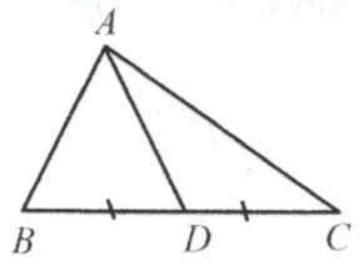
\includegraphics[max width=\textwidth, center]{2025_04_17_97bc1f7e44d93c271a88g-007(1)}

Theorem 1.1. The medians of a triangle meet at a point that is two-thirds of the distance from any vertex to the midpoint of the opposite side.

\[
A G=\frac{2}{3} A D, \quad B G=\frac{2}{3} B E, \quad C G=\frac{2}{3} C F .
\]

Proof:
Let \(E\) and \(F\) denote the midpoints of \(A C\) and \(A B\), respectively.\\
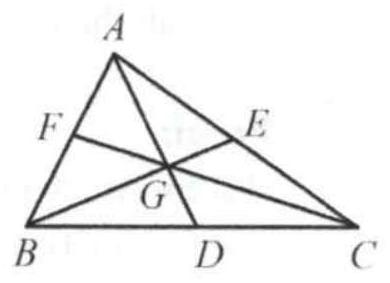
\includegraphics[max width=\textwidth, center]{2025_04_17_97bc1f7e44d93c271a88g-007(2)}

Connect \(E F . E F=\frac{1}{2} B C\) and \(E F / / B C\).\\
Since \(\triangle G E F \sim \triangle G B C, \frac{G E}{G B}=\frac{E F}{B C}\).\\
Since \(B C=2 E F, G B=2 G E\).\\
\(B G=\frac{2}{3} B E\).\\
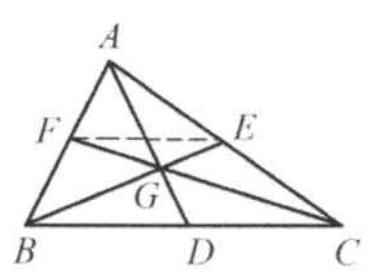
\includegraphics[max width=\textwidth, center]{2025_04_17_97bc1f7e44d93c271a88g-007}


Similarly, we can prove \(A G=\frac{2}{3} A D\) and \(C G=\frac{2}{3} C F\).\\
Theorem 1.2. Three medians divide the triangle \(A B C\) into six small triangles of equal areas.\\
\(S_{\triangle A D G}=S_{\triangle D C G G}=S_{\triangle C F G}=S_{\triangle F B G}=S_{\triangle B E G}=S_{\triangle E A G}=\frac{1}{6} S_{\triangle B B C}\)

Proof:
Since \(A D=D C, \frac{S_{\triangle A D G}}{S_{\triangle D C G}}=\frac{A D}{D C}=1 \quad \Rightarrow \quad S_{\triangle A D G}=S_{\triangle D C G}\).\\
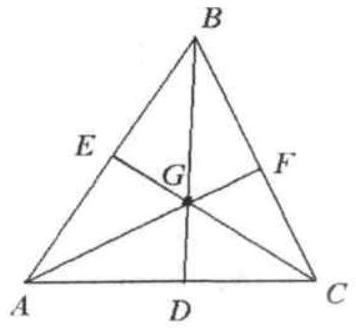
\includegraphics[max width=\textwidth, center]{2025_04_17_97bc1f7e44d93c271a88g-008(1)}

Since \(A G=2 G F, \frac{S_{\triangle C G F}}{S_{\triangle C A G}}=\frac{G F}{A G}=\frac{1}{2} \Rightarrow\)

\[
S_{\triangle C G F}=\frac{1}{2} S_{\triangle C A G}=S_{\triangle A D G}=S_{\triangle D C G} \text {. }
\]

Similarly, \(S_{\triangle A D G}=S_{\triangle D C G}=S_{\triangle C F G}=S_{\triangle F B G G}=S_{\triangle B E G}=S_{\triangle E A G}=\frac{1}{6} S_{\triangle A B C}\).

Theorem 1.3. The measure of the median on the hypotenuse of a right triangle is one-half the measure of the hypotenuse \((A M=M B=M C)\).

Proof:
We construct a rectangle \(A D B C\) as shown. We know that \(A B\) and \(C D\) are two diagonals and they are equal and bisect each\\
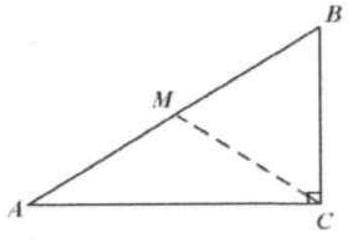
\includegraphics[max width=\textwidth]{2025_04_17_97bc1f7e44d93c271a88g-008(2)} other.

So \(D M=M C=A M=M B \quad \Rightarrow \quad A M=M B=M C\)\\
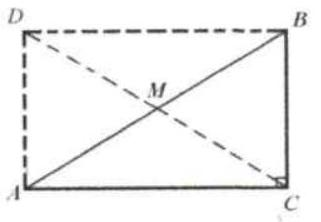
\includegraphics[max width=\textwidth, center]{2025_04_17_97bc1f7e44d93c271a88g-008}

The converse of this statement, if the median to a side of a triangle is one-half of the measure of that side, or \(A M=M B=M C\), then triangle \(A B C\) is a right triangle, is also true.

### CHAPTER 1 EXAMPLE 1-1 ###
Example 1. Show that for right triangle, if \(\angle A=30^{\circ}\), then \(B C=\frac{1}{2} A B\).

Proof:
Draw the median \(M C\). Since \(M C\) is the median, \(M C=\) \(A M=M B\).\\
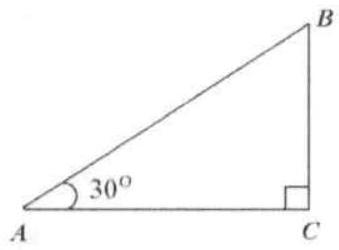
\includegraphics[max width=\textwidth, center]{2025_04_17_97bc1f7e44d93c271a88g-009(4)}

Triangle \(A M C\) is an isosceles triangle with \(\angle M A C=\angle M C A=30^{\circ}\).

Since \(\angle B M C\) is the exterior angle of triangle \(A M C\), \(\angle B M C=\angle M A C+\angle M C A=30^{\circ}+30^{\circ}=60^{\circ}\).\\
So, triangle \(M B C\) is an equilateral triangle with \(B C=\) \(M C=M B\).\\
That is \(B C=\frac{1}{2} A B\).\\
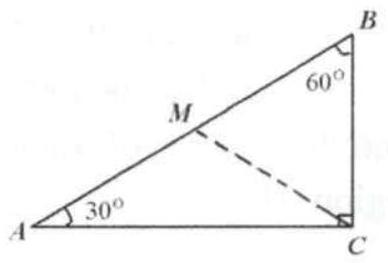
\includegraphics[max width=\textwidth, center]{2025_04_17_97bc1f7e44d93c271a88g-009(3)}

Example 2. In right triangle \(A B C, M\) and \(N\) are midpoints of legs \(\overline{A B}\) and \(\overline{B C}\), respectively. Leg \(\overline{A B}\) is 6 units long, and leg \(\overline{B C}\) is 8 units long. How many square units are in the area of \(\triangle A P C\) ? (Mathcounts Competitions)

Solution: 8 (square units)\\
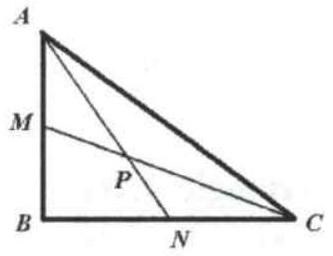
\includegraphics[max width=\textwidth, center]{2025_04_17_97bc1f7e44d93c271a88g-009(1)}

We draw the third median \(B D\).

These three medians divide the triangle into six equal areas. The area of triangle \(A B C\) is \(6 \times 8 / 2=24\).\\
The area of \(\triangle A P C\) is just \(\frac{2}{6} \times 24=8\).\\
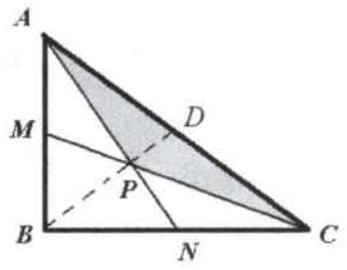
\includegraphics[max width=\textwidth, center]{2025_04_17_97bc1f7e44d93c271a88g-009}

Example 3. In right \(\triangle A B C, \angle B=90^{\circ}, \angle B A C=78^{\circ}\). Draw \(C F / / A B\). Connect \(A F\) and \(B C\). \(B C\) and \(A F\) meet at \(G\). If \(F G=2 A C\), find \(\angle B A G\).\\
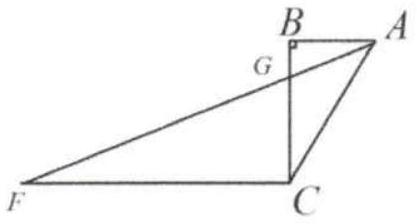
\includegraphics[max width=\textwidth, center]{2025_04_17_97bc1f7e44d93c271a88g-009(2)}


Solution: \(26^{\circ}\).\\
Since \(A B / / C F, \angle F C B=90^{\circ} . \triangle F B C\) is a right triangle.\\
Take \(E\), the midpoint of \(F G\). Connect \(E C\).\\
\(E C=\frac{1}{2} F G=A C\).\\
Thus \(\angle E A C=\angle A E C=\angle F+\angle E C F=2 \angle F\).\\
Let \(\angle B A G=x . \angle F=x\).\\
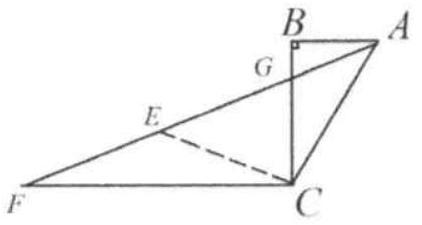
\includegraphics[max width=\textwidth, center]{2025_04_17_97bc1f7e44d93c271a88g-010(2)}

So, \(x+2 x=78^{\circ} \quad \Rightarrow \quad x=26^{\circ}\).\\
Example 4. (NYML) 234 is the inch-length of the altitude to base \(A C\) of isosceles triangle \(A B C\). If the inch-length of the median to \(B C\) is 195 , find the number of square inches in the area of triangular region \(A B C\).

Solution: 24336.
We draw the third median \(C E\).\\
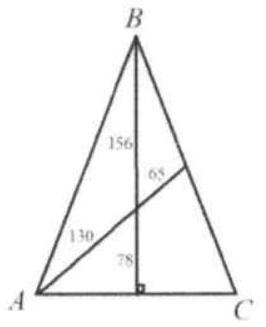
\includegraphics[max width=\textwidth, center]{2025_04_17_97bc1f7e44d93c271a88g-010(1)}\\
\(A F, C E\), and \(B D\) are three medians. They meet at \(G\).\\
\(G D=\frac{1}{3} B D=\frac{1}{3} \times 234=78 . A G=\frac{2}{3} A F=\frac{2}{3} \times 195=130\).\\
Triangle \(A D G\) is a 3-4-5 right triangle \((3 \times 26,4 \times 26,5 \times 26)\) and \(A D=104\).\\
\(S_{\triangle A D G}=\frac{78 \times 104}{2}=4056\)\\
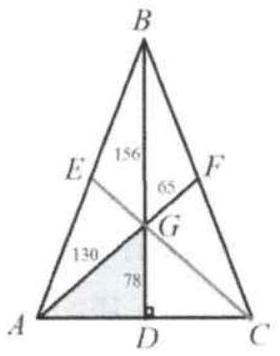
\includegraphics[max width=\textwidth, center]{2025_04_17_97bc1f7e44d93c271a88g-010}\\
\(S_{\triangle A B C}=6 S_{\triangle A D G}=6 \times 4056=24336\).\\
Example 5. (AMC) Medians \(B D\) and \(C E\) of a triangle \(A B C\) are perpendicular, \(B D\) \(=8\), and \(C E=12\). Find the area of triangle \(A B C\).

Solution: 64.
We draw the third median \(A F\).\\
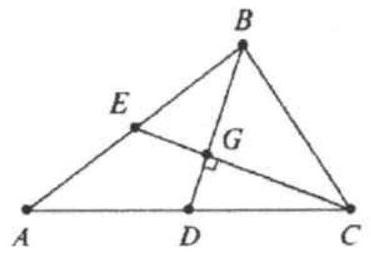
\includegraphics[max width=\textwidth, center]{2025_04_17_97bc1f7e44d93c271a88g-010(3)}


\(C D=C D=\frac{1}{2} C M=\frac{4}{2}=2\).

Example 8. \(A B C D\) is a rectangle with \(A B=2 B C\). \(E\) and \(F\) are the midpoints of \(A B\) and \(A D\), respectively. \(D E\) and \(B F\) meet at \(G\). What is the ratio of the area of \(G B C D\) to the area of \(A B C D\) ?\\
(A) \(\frac{5}{2}\)\\
(B) \(\frac{2}{5}\)\\
(C) \(\frac{2}{3}\)\\
(D) \(\frac{4}{5}\)\\
(E) \(\frac{3}{5}\)\\
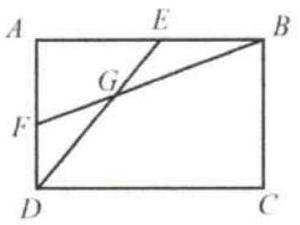
\includegraphics[max width=\textwidth, center]{2025_04_17_97bc1f7e44d93c271a88g-011}

Solution: (C).\\
We connect \(B D\) and extend \(A G\) to meet \(B D\) at \(H\).\\
Since the medians \(D E\) and \(B F\) meet at \(G, G\) is the centroid of triangle \(A B D\) and the six small triangles formed have the same area.\\
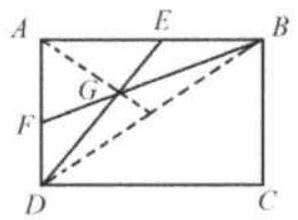
\includegraphics[max width=\textwidth, center]{2025_04_17_97bc1f7e44d93c271a88g-011(1)}

Each of the small triangles has an area that is \(\frac{1}{12}\) of the area of the rectangle \(A B C D\), so the area of triangle \(D B G, S_{D G B}=\frac{2}{12} \times S_{A B C D}\).\\
The area of triangle \(D B C, S_{D B C}=\frac{1}{2} \times S_{A B C D}\).\\
\(S_{D C B C}=S_{D C B}+S_{D B C}=\frac{2}{12} S_{A B C D}+\frac{1}{2} S_{A B C D}=\left(\frac{2}{12}+\frac{1}{2}\right) \times S_{A B C D}\).\\
The ration of the area of \(G B C D\) to the area of \(A B C D\).\\
\(S_{D C B C}=\frac{S_{D C B C}}{S_{A B C D}}=\frac{2}{12}+\frac{1}{2}=\frac{2+6}{12}=\frac{2}{3}\).

Example 9. \(\triangle A B C\) is a right triangle with \(\angle A C B=90^{\circ}\). Points \(D\) and \(E\) are the midpoints on sides \(A B\) and \(A C\), respectively. Extend \(B C\) to \(F\) such that \(C F=\frac{1}{2} B C\). Connect \(C F\). Show that \(\angle B=\angle F\).\\
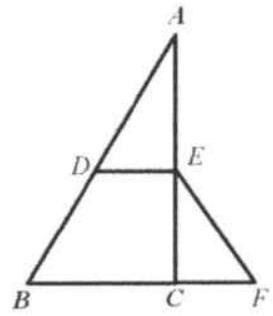
\includegraphics[max width=\textwidth, center]{2025_04_17_97bc1f7e44d93c271a88g-011(2)}


Solution:
Draw \(D C\), the median of triangle \(A B C\). Since \(D C\) is the median, by Theorem 1.3, \(D C=B D\).\\
Since \(A D=\frac{1}{2} F C, A D=D N\). So that \(\angle B=\angle D C B\).\\
Since points \(D\) and \(E\) are the midpoints on sides \(A B\) and \(A C\), \(D E=\frac{1}{2} B C=C F\) and \(D E / / B C\). Thus \(D E F C\) is a\\
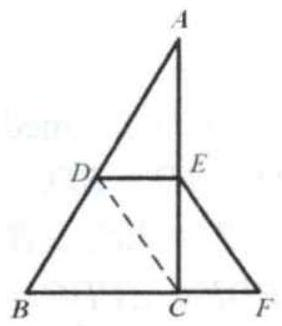
\includegraphics[max width=\textwidth]{2025_04_17_97bc1f7e44d93c271a88g-012} parallelogram. So \(D C / / E F\) and \(\angle D C B=\angle F\).\\
Since \(\angle B=\angle D C B, \angle B=\angle F\).

Example 10. \(A B C D\) is a parallelogram. \(D E \perp A B\) at \(E . A D=\frac{1}{2} F C\). Show that \(\angle D A B=3 \angle A C D\).

Solution:
\begin{center}
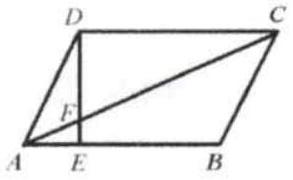
\includegraphics[max width=\textwidth]{2025_04_17_97bc1f7e44d93c271a88g-012(1)}
\end{center}

Draw \(D N\), the median of triangle \(C D F\). Since \(D N\) is the median, by Theorem 1.3, \(D N=F N=N C\).\\
Since \(A D=\frac{1}{2} F C, A D=D N\).\\
Thus triangle \(A N D\) is an isosceles triangle with \(\angle D A N=\angle D N A\).\\
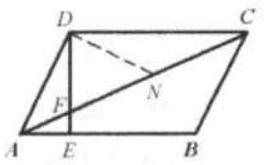
\includegraphics[max width=\textwidth, center]{2025_04_17_97bc1f7e44d93c271a88g-012(2)}

We also know that \(D N=N C\), so \(\angle N D C=\angle N C D\).\\
\(\angle D N A\) is the exterior angle of triangle \(D N C\). So \(\angle D N A=\angle N D C+\angle N C D\)\\
\(=2 \angle N C D\).\\
Note that \(\angle C A B=\angle N C D\).\\
Therefore \(\angle D A B=\angle D C A+\angle C A B=\angle D N A+\angle N C D\)\\
\(=2 \angle N C D+\angle N C D=3 \angle N C D=3 \angle A C D\).

Example 11. \(\triangle A B C\) is a right isosceles triangle with \(\angle A C B=90^{\circ}\) and \(A C=B C\).\\
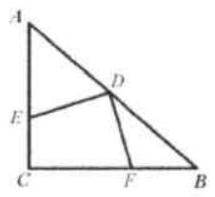
\includegraphics[max width=\textwidth, center]{2025_04_17_97bc1f7e44d93c271a88g-012(3)}

Point \(D\) is the midpoints on sides \(A B . D E \perp D F\). Points \(E, F\) are on sides \(A C\) and \(B C\), respectively. Show that \(D E=D F\).

Solution:
Draw \(C D\), the median of triangle \(A B C\). Since \(C D\) is the median, by Theorem 1.3, \(C D=A D=B D\).\\
\(\angle A C D=45^{\circ} . \angle B=45^{\circ}\).\\
\(\angle B D F+\angle F D C=90^{\circ}\).\\
\(\angle F D C+\angle C D E=90^{\circ}\).\\
\(\angle B D F=\angle C D E=\alpha\).\\
\(\angle A C D=\angle E C D=\angle B=45^{\circ}\).\\
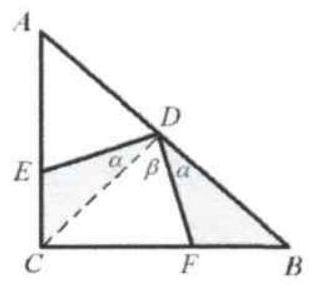
\includegraphics[max width=\textwidth, center]{2025_04_17_97bc1f7e44d93c271a88g-013}\\
\(\triangle C E D \cong \triangle B F D\).\\
Thus \(D E=D F\).

Example 12. \(\triangle A B C\) is an isosceles right triangle with \(\angle A=90^{\circ}\). Points \(P\) and \(Q\) are points on sides \(A B\) and \(A C\), respectively. \(B P=A Q\). Show that \(\triangle P D Q\) is also an isosceles right triangle if \(D\) is the midpoint of \(B C\).

Solution:
Draw the median \(A D\).\\
Since \(\triangle A B C\) is an isosceles right triangle and \(D\) is the midpoint of \(B C, A D \perp B C, \angle A D C=90^{\circ}\).\\
By Theorem 1.3, \(A D=B D=D C . \angle D A Q=\angle A=45^{\circ}\).\\
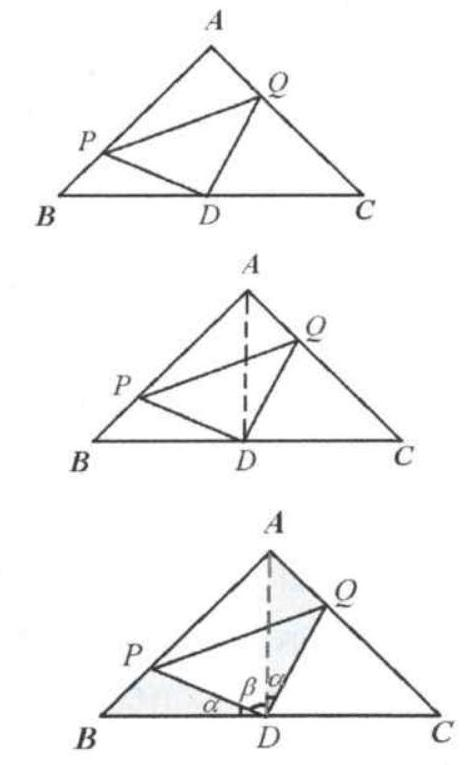
\includegraphics[max width=\textwidth, center]{2025_04_17_97bc1f7e44d93c271a88g-013(1)}

Since \(B P=A Q, \triangle B P D \cong \triangle A Q D\).\\
Thus, \(P D=Q D . \angle A D Q=\angle B D P=\alpha\).\\
We see that \(\angle A D Q=\alpha+\beta=90^{\circ}\).\\
So \(\angle P D Q=\alpha+\beta=90^{\circ}\).

We also know that \(P D=Q D\).\\
Thus \(\triangle P D Q\) is an isosceles right triangle.


Example 13. Let \(M\) be the midpoint of side \(A B\) of triangle \(A B C\). Let \(P\) be a point on \(A B\) between \(A\) and \(M\), and let \(M D\) be drawn parallel to \(P C\) and intersecting \(B C\) at \(D\). If the ratio of the area of triangle \(B P D\) to that of triangle \(A B C\) is denoted by \(r\), then\\
(A) \(\frac{1}{2}<r<1\) depending upon the position of \(P\)\\
(B) \(r=\frac{1}{2}\) independent of the position of \(P\)\\
(C) \(\frac{1}{2} \leq r<1\) depending upon the position of \(P\)\\
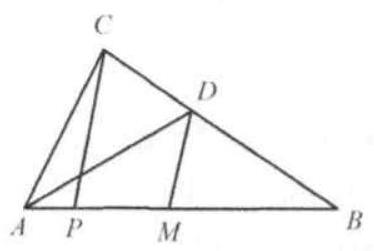
\includegraphics[max width=\textwidth, center]{2025_04_17_97bc1f7e44d93c271a88g-014(1)}\\
(D) \(\frac{1}{3}<r<\frac{2}{3}\) depending upon the position of \(P\)\\
(E) \(r=\frac{1}{3}\) independent of the position of \(P\)

Solution: (B).\\
Let \(r=\frac{S_{\triangle B P D}}{S_{\triangle A B C}}\)\\
Draw the median \(C M\). Connect \(D P\). Let the intersection point be \(N\).\\
Since \(P C / / M D, S_{\triangle C D N}=S_{\triangle M P N}\).\\
Thus \(S_{\triangle B P D}=S_{\triangle B C M}\)\\
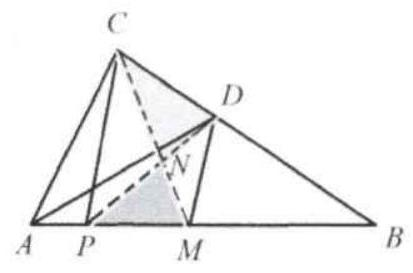
\includegraphics[max width=\textwidth, center]{2025_04_17_97bc1f7e44d93c271a88g-014}

Since \(C M\) is the median, \(S_{\triangle B P D}=S_{\triangle B C M}=\frac{1}{2} S_{\triangle A B C}\)\\
Substituting (2) into (1): \(r=\frac{S_{\triangle B P D}}{S_{\triangle A B C}}=\frac{1}{2}\).


### CHAPTER 1 PROBLEMS 1-1 ###

Problem 1. (AMC) Let line \(A C\) be perpendicular to line \(C E\). Connect \(A\) to the midpoint \(D\) of \(C E\), and connect \(E\) to the midpoint \(B\) of \(A C\). If \(A D\) and \(E B\) intersect in point \(F\), and \(B C=C D=15\) inches, find the area of triangle \(D F E\) in square inches.

Problem 2. Triangle \(A B C\) is an isosceles triangle. \(B D\) is the altitude to base \(A C\). \(A F\) is the median to \(B C . A F\) meets \(B D\) at \(G\). Find the number of square inches in the area of triangle \(A B G\) if \(B D=234\) and \(A F=195\).\\
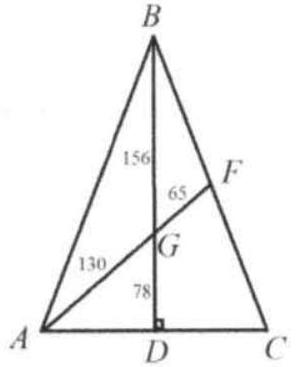
\includegraphics[max width=\textwidth, center]{2025_04_17_97bc1f7e44d93c271a88g-015(1)}

Problem 3. Medians \(B D\) and \(C E\) of a triangle \(A B C\) are perpendicular, \(C E=24\) and the area of triangle \(A B C\) is 288 . Find the length of \(B D\).\\
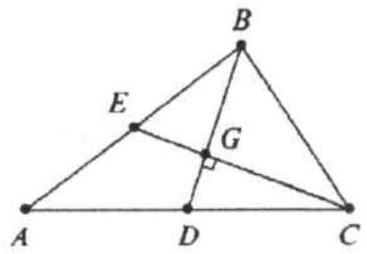
\includegraphics[max width=\textwidth, center]{2025_04_17_97bc1f7e44d93c271a88g-015(2)}

Problem 4. ( \(A M C\) ) In the obtuse triangle \(A B C, A M=M B, M D \perp B C, E C \perp B C\). If the area of \(\triangle A B C\) is 24 , find the area of \(\triangle B E D\).\\
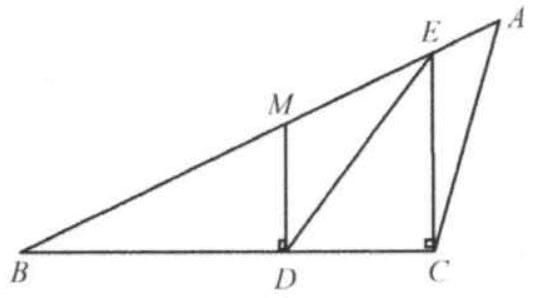
\includegraphics[max width=\textwidth, center]{2025_04_17_97bc1f7e44d93c271a88g-015}


Problem 5. In \(\triangle A B C\), angle \(C\) is a right angle. \(A C\) and \(B C\) are each equal to 1. \(D\) is the midpoint of \(A C . B D\) is drawn, and a line perpendicular to \(B D\) at \(P\) is drawn from \(C\). Find the distance from \(P\) to the intersection of the medians of \(\triangle A B C\).\\
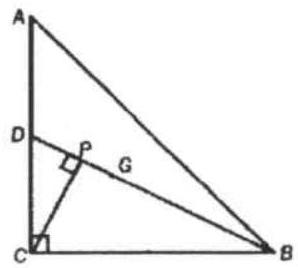
\includegraphics[max width=\textwidth, center]{2025_04_17_97bc1f7e44d93c271a88g-016(4)}

Problem 6. In \(\triangle A B C, \angle B=2 \angle A\) and \(A B=2 B C\). Show that \(A B^{2}=A C^{2}+B C^{2}\).\\
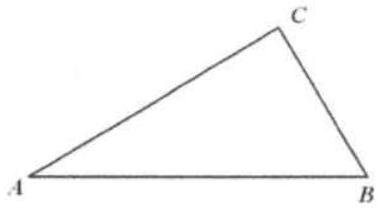
\includegraphics[max width=\textwidth, center]{2025_04_17_97bc1f7e44d93c271a88g-016}

Problem 7. \(A B C D\) is a quadrilateral with \(A D / / B C\). Draw \(A G \perp A B\) to meet \(D C\) at \(F\) and the extension of \(B C\) at \(G\). Points \(E\) is the midpoint of sides \(B G\). Find the length \(A E\) if \(A D=\) 2.7, \(A F=4\), and \(A B=6\).\\
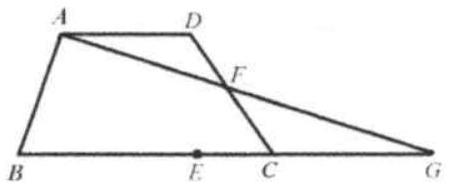
\includegraphics[max width=\textwidth, center]{2025_04_17_97bc1f7e44d93c271a88g-016(1)}

Problem 8. As shown in the figure, \(A B / / C D . A D \perp A B . A D\) and \(B C\) meet at \(E\) such that \(E B=2 A C\). Show that \(\angle A C D=3 \angle B C D\).\\
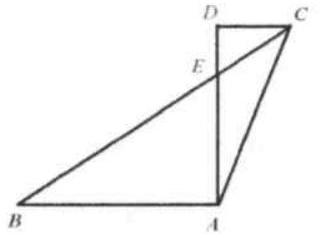
\includegraphics[max width=\textwidth, center]{2025_04_17_97bc1f7e44d93c271a88g-016(2)}

Problem 9. Both \(\triangle A B C\) and \(\triangle A D C\) are right triangles sharing the hypotenuse \(A C\) with \(\angle A B C=\angle A D C=90^{\circ}\). Points \(M\) and \(n\) are the midpoints on sides \(A C\) and \(B D\), respectively. Show that \(M N \perp B D\).\\
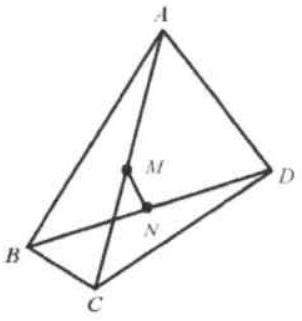
\includegraphics[max width=\textwidth, center]{2025_04_17_97bc1f7e44d93c271a88g-016(3)}


### CHAPTER 1 SOLUTIONS 1-1 ###
Problem 1. Solution: (C).\\
Method 1 (official solution):\\
Draw \(A E\) and the altitude \(F G\) to the base \(D E\) of triangle \(D E F\). Since \(F\) is the intersection point of the medians of a triangle \(A C E, F D=\frac{1}{3} A D\).\\
\(\therefore F G=\frac{1}{3} A C=\frac{1}{3} \cdot 30=10\).\\
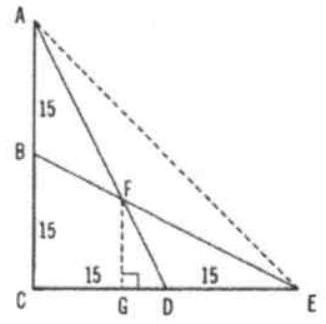
\includegraphics[max width=\textwidth, center]{2025_04_17_97bc1f7e44d93c271a88g-017(1)}\\
\(\therefore \operatorname{area}(\triangle D E F)=\frac{1}{2} \cdot 15 \cdot 10=75\).\\
The three medians of a triangle divide the triangle into six triangles of equal area. Therefore, \(\operatorname{Area}(\triangle F D E)=75\).

Method 2 (our solution):\\
Connect \(A E\). Then connect \(C F\) and extend it to meet \(A E\) at \(M\). \(F\) is the centroid and triangle \(A C E\) is divided into six smaller triangles with the same area.\\
The area of \((\triangle A C D)=\frac{1}{2} \cdot 30 \cdot 15=225\). The area of\\
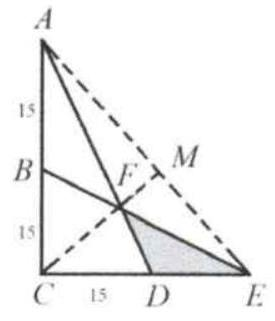
\includegraphics[max width=\textwidth]{2025_04_17_97bc1f7e44d93c271a88g-017} \((\triangle F D E)=\frac{225}{3}=75\).

Problem 2. Solution: 8112.\\
Method 1:\\
\(A F, C E\), and \(B D\) are three medians. They meet at \(G\). Triangle \(A B C\) is divided into six smaller equal areas. \(G D=\frac{1}{3} B D=\frac{1}{3} \times 234=78 . A G=\frac{2}{3} A F=\frac{2}{3} \times 195=130\).\\
Triangle \(A D G\) is a 3-4-5 right triangle \((3 \times 26,4 \times 26,5 \times 26)\) and \(A D=104\).\\
\(S_{\triangle A D G}=\frac{78 \times 104}{2}=4056\)\\
\(S_{\triangle A B G}=2 S_{\triangle M D G}=2 \times 4056=8112\).

Method 2:\\
Note that \(A B C\) is an isosceles triangle, so the altitude is also a median.\\
\(G D=\frac{1}{3} B D=\frac{1}{3} \times 234=78 . A G=\frac{2}{3} A F=\frac{2}{3} \times 195=130\).\\
\(A D=\sqrt{A G^{2}-D G^{2}}=\sqrt{130^{2}-78^{2}}=104\). The area of triangle \(A D G\) is \(S_{\triangle A D G}=\frac{78 \times 104}{2}=4056\).\\
\(\frac{S_{A B G G}}{S_{\triangle A D G}}=\frac{B G}{D G}=2\)\\
\(S_{\triangle A D G}=2 S_{\triangle A D G}=2 \times 4056=8112\).\\
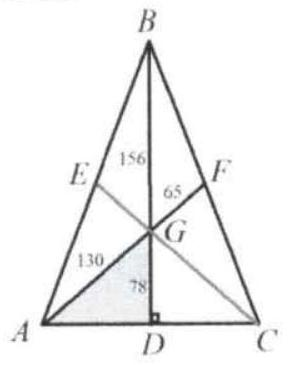
\includegraphics[max width=\textwidth, center]{2025_04_17_97bc1f7e44d93c271a88g-018(4)}

Problem 3. Solution: 18.\\
\(D G=\frac{1}{3} B D\), and \(C G=\frac{2}{3} C E=\frac{2}{3} \times 24=16\)\\
\(S_{\triangle C D G G}=\frac{1}{2} D G \times C G=\frac{1}{2} \times \frac{1}{3} B D \times 16=\frac{8}{3} B D\)\\
We know that \(S_{\triangle C D G}=\frac{1}{6} S_{\triangle A B C}\)\\
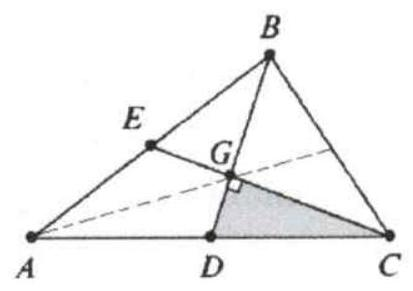
\includegraphics[max width=\textwidth, center]{2025_04_17_97bc1f7e44d93c271a88g-018(3)}\\
\(\Rightarrow \quad S_{\triangle C D G}=\frac{8}{3} B D=\frac{1}{6} \times 288 \Rightarrow B D=18\).

Problem 4. Solution: 12.
Draw the median MC (Figure 1).\\
Since \(M D\) and \(E C\) are parallel, the colored areas in Figure 2 are the same. The area of \(\triangle B E D\) is the same as the area of \(\triangle B M C\) (Figure 3), which is half of the area of \(\triangle A B C\). The answer is \(24 / 2=12\).\\
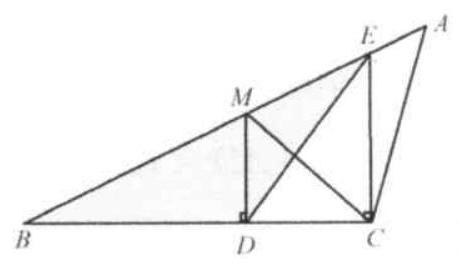
\includegraphics[max width=\textwidth, center]{2025_04_17_97bc1f7e44d93c271a88g-018(2)}

Figure 1\\
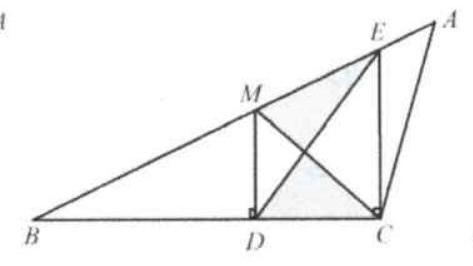
\includegraphics[max width=\textwidth, center]{2025_04_17_97bc1f7e44d93c271a88g-018}

Figure 2\\
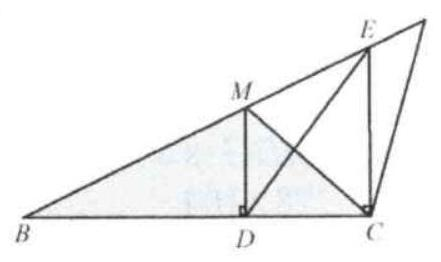
\includegraphics[max width=\textwidth, center]{2025_04_17_97bc1f7e44d93c271a88g-018(1)}

Figure 3


Problem 5. Solution: \(\frac{1}{15} \sqrt{5}\).\\
Applying the Pythagorean Theorem to \(\triangle D C B\) gives us\\
\((D C)^{2}+(C B)^{2}=(D B)^{2}\).\\
\(1 / 4+1=(D B)^{2}, D B=\frac{1}{2} \sqrt{5}\).\\
Since the centroid of a triangle trisects each of the medians,\\
\(D G=\frac{1}{3} D B=\frac{1}{3}\left(\frac{1}{2} \sqrt{5}\right)=\frac{1}{6} \sqrt{5}\)\\
Consider right \(\triangle D C B\) where \(C P\) is the altitude drawn upon the hypotenuse.\\
Therefore, \(D B / D C=D C / D P . \frac{\frac{1}{2} \sqrt{5}}{\frac{1}{2}}=\frac{\frac{1}{2}}{D P}, D P=\frac{\sqrt{5}}{10}\)\\
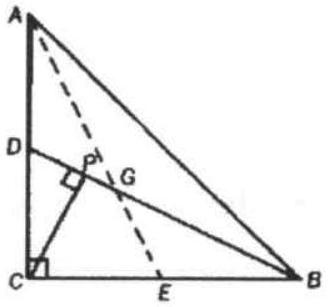
\includegraphics[max width=\textwidth, center]{2025_04_17_97bc1f7e44d93c271a88g-019}

Thus, \(P G=D G-D P\), and \(P G=\frac{1}{6} \sqrt{5}-\frac{1}{10} \sqrt{5}=\frac{1}{15} \sqrt{5}\).

Problem 6. Solution:
Since \(A B>B C, \angle C>\angle A\).\\
Draw \(C D\) to meet \(A B\) at \(D\) such that \(\angle A C D=\angle A\).\\
\(\triangle A D C\) is an isosceles triangle and \(A D=D C\).\\
\(\angle C D B=\angle A C D+\angle A=2 \angle A=\angle B\)\\
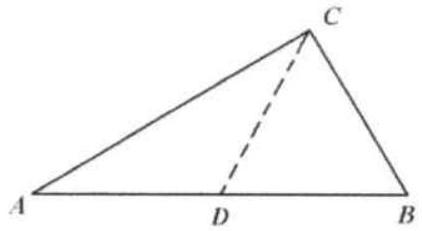
\includegraphics[max width=\textwidth, center]{2025_04_17_97bc1f7e44d93c271a88g-019(1)}

Therefore, \(\triangle B C D\) is also an isosceles triangle, and so \(D C=B C\).\\
\(A B=A D+D B=2 B C\)\\
\(\Rightarrow \quad A D+D B=2 D C=2 A D\)\\
\(\Rightarrow \quad A D=D B=D C\).

This tells us that \(D C\) is the median of right triangle \(A B C\) with \(\angle C=90^{\circ}\).\\
By the Pythagorean Theorem, we have \(A B^{2}=A C^{2}+B C^{2}\).


Problem 7. Solution: 5.\\
Draw \(A E\). Since \(A E\) is the median, by Theorem \(1.3, A E=B E=E G\).

Since \(A D / / B C, \angle D A F=\angle C G F\).\\
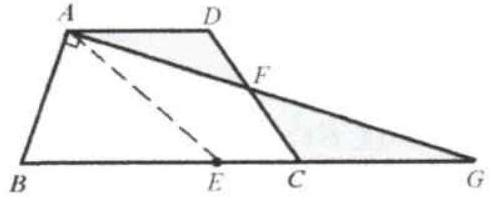
\includegraphics[max width=\textwidth, center]{2025_04_17_97bc1f7e44d93c271a88g-020}\\
\(\angle D F A=\angle C F G\) (vertical angles).\\
\(\angle A D F=\angle G C F\).\\
Thus \(\triangle A D F \cong \triangle G C F . A F=F G=4\).\\
Triangle \(A B G\) is a \(6-8-10\) right triangle. \(B E=\frac{1}{2} B G=5\).\\
The answer is \(A E=B E=5\).

Problem 8. Solution:
Draw \(A F\), the median of right triangle \(B A E\). Since \(A F\) is the median, by Theorem 1.3, \(A F=B F=N C\).\\
Thus \(A F=A C\).\\
Thus both triangles \(A F B\) and \(C A F\) are isosceles triangles.\\
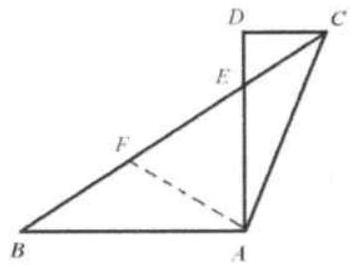
\includegraphics[max width=\textwidth, center]{2025_04_17_97bc1f7e44d93c271a88g-020(3)}

Let \(\angle B=\angle F A B=\alpha\).\\
\(\angle C F A\) is the exterior angle of triangle \(A B F\). So \(\angle C F A=\) \(\angle A C F=2 \alpha\).\\
Since \(A B / / C D, \angle B=\angle D C E=\alpha\).\\
\(\angle A C D=\angle A C F+\angle D C E=3 \alpha=3 \angle B C D\).\\
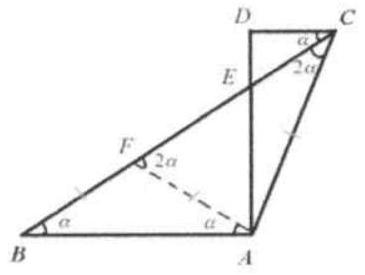
\includegraphics[max width=\textwidth, center]{2025_04_17_97bc1f7e44d93c271a88g-020(2)}

Problem 9. Solution:
Draw \(M B\), the median of triangle \(A B C\). Since \(M B\) is the median, by Theorem 1.3, \(M B=M A=M C\)

Draw \(M D\), the median of triangle \(A D C\). Since \(M D\) is the median, by Theorem 1.3, \(M D=M A=M C\). So \(M B=M D\).\\
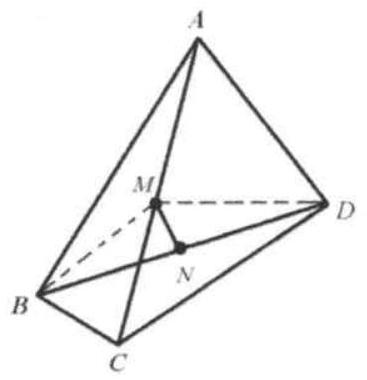
\includegraphics[max width=\textwidth, center]{2025_04_17_97bc1f7e44d93c271a88g-020(1)}


Since \(M B=M D\) and \(B N=N D, M N\) is the perpendicular bisector of \(B D\).\\
Thus \(M N \perp B D\).

Problem 10. Solution:
Draw \(D N\), the median of triangle \(A D C\).\\
\(N D=N C\).\\
Triangle \(N D C\) is an isosceles triangle with\\
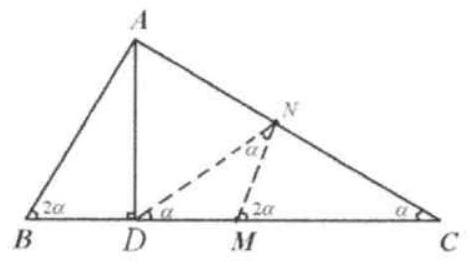
\includegraphics[max width=\textwidth]{2025_04_17_97bc1f7e44d93c271a88g-021(1)} \(\angle N D C=\angle C=\alpha\).\\
Connect \(M N\).\\
Since \(M\) is the midpoint of \(B C\) and \(N\) is the midpoint of \(A C, A B=2 M N\) and \(A B / /\) \(M N\).\\
Thus \(\angle N M C=\angle B=2 \angle C=2 \alpha\).\\
\(\angle D N M=2 \alpha-\alpha=\alpha\).\\
So \(D M=M N\).\\
\(A B=2 M N=2 D M\).

Problem 11. Solution:
Draw \(A E\), the median of right triangle \(A B D\).\\
\(A E=B E=E D\).\\
\(B D=2 A E\).\\
Since \(\angle B=15^{\circ}\), and \(\triangle A B E\) is an isosceles triangle, \(\angle E A D=15^{\circ}\).\\
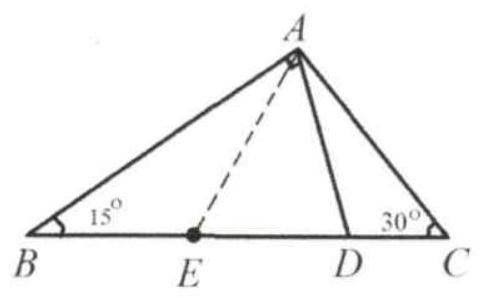
\includegraphics[max width=\textwidth, center]{2025_04_17_97bc1f7e44d93c271a88g-021}

Since \(\angle A E D\) is an exterior angle of \(\triangle A B E, \angle A E D=30^{\circ}\).\\
Then we know that \(\triangle A E C\) is an isosceles triangle with \(A E=A C\).\\
Therefore \(B D=2 A E=2 A C\).

Problem 12. Solution:
Draw \(E O\), the median of triangle \(A E C\). Since \(E O\) is the median, by Theorem 1.3, \(E O=A O=O C\).


Note that \(E O\) is also the median of triangle \(B E D\). Since \(E O\) is the median, by Theorem 1.3, \(E O=B O=O D\).\\
Thus \(A C=B D\) and \(A B C D\) is a rectangle.\\
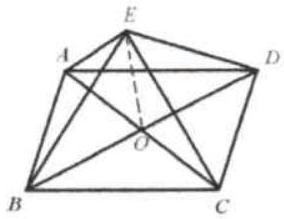
\includegraphics[max width=\textwidth, center]{2025_04_17_97bc1f7e44d93c271a88g-022}

Problem 13. Solution: \(65^{\circ}\).\\
Since Thus \(\angle A B C=75^{\circ}, \angle B A F=90^{\circ}-75^{\circ}=15^{\circ}\).

Take \(G\), the midpoint of \(E D\). Connect \(A G\).\\
Since \(A F \perp B C\), and \(A D / / B C, A F \perp A D\).\\
\(\triangle A D E\) is a right triangle and \(A G\) is the median on\\
\(E D\). So \(A G=G D=\frac{1}{2} D E=A B\).\\
So \(\angle G A D=\angle G D A=\alpha\).\\
\includegraphics[max width=\textwidth, center]{2025_04_17_97bc1f7e44d93c271a88g-022(1)}

So \(\angle A G E=2 \alpha=\angle A B G\).

Since \(A B C D\) is a parallelogram. \(\angle C B D=\angle A D B=\alpha\).

Thus \(\angle A B C=75^{\circ}=3 \alpha \quad \Rightarrow \quad \alpha=75^{\circ} / 3=25^{\circ}\). \(\angle A E D=2 \alpha+15^{\circ}=65^{\circ}\).


2. Double the length of the median of a triangle.
In triangle \(A B C, A M\) is the median on side \(B C\). If we extend \(A M\) to \(N\) such that \(A M=M N\) and connect \(N\), we get two congruent triangles \(\triangle A M C\) and \(\triangle N M B\). \((S A S: A M=M N, B M=M C, \angle A M C=\) \(\angle N M B\) ).\\
\includegraphics[max width=\textwidth, center]{2025_04_17_97bc1f7e44d93c271a88g-023}

### CHAPTER 1 EXAMPLE 1-2 ###

Example 1. Prove that the sum of any two sides of a triangle is greater than twice the length of median drawn to the third side.

Proof:
As shown in the figure, in \(\triangle A B C, A D\) is the median. We want to prove that \(A D<\frac{1}{2}(A B+A C)\).\\
\includegraphics[max width=\textwidth, center]{2025_04_17_97bc1f7e44d93c271a88g-023(1)}

Extend \(A D\) to \(E\) such that \(A D=D E\).\\
Connect BE.

Since \(D E=A D, \angle B D E=\angle C D A . B D=D C\).\\
Thus \(\triangle B D E \cong \triangle C D A, B E=A C\),\\
In \(\triangle A B E, A B+B E>A E=2 A D\).\\
So \(A D<\frac{1}{2}(A B+B E)\).\\
\includegraphics[max width=\textwidth, center]{2025_04_17_97bc1f7e44d93c271a88g-023(2)}

Since \(B E=A C\), we have \(A D<\frac{1}{2}(A B+A C)\).


Example 2. Show that the measure of the median on the hypotenuse of a right triangle is one-half the measure of the hypotenuse ( \(A M\) \(=M B=M C\) ).

Proof:
Extend \(C M\) to \(D\) such that \(C M=D M\).\\
\includegraphics[max width=\textwidth, center]{2025_04_17_97bc1f7e44d93c271a88g-024(2)}

Connect \(B D\) and \(A D\).\\
\(A B\) and \(C D\) are two diagonals and they bisect each other. So \(A C B D\) is a parallelogram.

Since \(\angle C=90^{\circ}, A C B D\) is a rectangle.\\
\includegraphics[max width=\textwidth, center]{2025_04_17_97bc1f7e44d93c271a88g-024(1)}

Thus \(D M=M C=A M=M B\).

Example 3. In \(\triangle A B C, \angle B A D=30^{\circ} . \angle B A C=120^{\circ} . D\) is the midpoint of \(B C\). Prove: \(A B=2 A C\).

Solution:
\begin{center}
\includegraphics[max width=\textwidth]{2025_04_17_97bc1f7e44d93c271a88g-024(4)}
\end{center}

Extend \(A D\) to \(E\) such that \(A D=D E\). Connect \(B E\).

Since \(D E=A D, \angle B D E=\angle C D A . B D=D C\).\\
Thus \(\triangle B D E \cong \triangle C D A, B E=A C\), and \(\angle E=\angle D A C\).\\
\includegraphics[max width=\textwidth, center]{2025_04_17_97bc1f7e44d93c271a88g-024}

Since \(\angle B A C=120^{\circ}, \angle B A D=30^{\circ}, \angle D A C=\angle B A C-\angle B A D=90^{\circ}\).\\
Thus, \(\angle E=90^{\circ}\).\\
Since \(\angle B A D=30^{\circ}, A B=2 A C\).

Example 4. In \(\triangle A B C, A B=7 . A C=11 . A D\) is the median on side \(B C\). How many integer values are there of \(A D\) ?

Solution: 6.\\
\includegraphics[max width=\textwidth, center]{2025_04_17_97bc1f7e44d93c271a88g-024(3)}


Extend \(A D\) to \(E\) such that \(A D=D E\).\\
Connect \(B E\).

Since \(D E=A D, \angle B D E=\angle C D A . B D=D C\).\\
Thus \(\triangle B D E \cong \triangle C D A, B E=A C=11\).

By the triangle inequality theorem,\\
\includegraphics[max width=\textwidth, center]{2025_04_17_97bc1f7e44d93c271a88g-025(1)}\\
\(11-7<A E<11+7 \Rightarrow 4<2 A D<18 \Rightarrow \quad 2<A D<9\).\\
There are six possible values: \(3,4,5,6,7\), and 8 .

Example 5. In \(\triangle A B C, A M\) is the median. \(A B G F\) and \(A C D E\) are squares. Prove:\\
\(E F=2 A M\).

Solution:
Extend \(A M\) to \(N\) such that \(A M=M N\).\\
Connect \(B N\).\\
\includegraphics[max width=\textwidth, center]{2025_04_17_97bc1f7e44d93c271a88g-025(2)}

Since \(B M=C M, A M=M N\), and \(\angle A M C=\angle N M B\), we have \(\triangle A M C \cong \triangle N M B\).

Thus \(B N=A C, \angle M N B=\angle M A C=\alpha\),\\
Connect \(E F\).\\
\(\angle E A F=360^{\circ}-90^{\circ}-90^{\circ}-\angle B A M-\angle M A C\)\\
\(=180^{\circ}-\beta-\alpha\).\\
\(\angle A B N=180^{\circ}-\angle B A M-\angle M N B\).\\
Since \(\angle M N B=\angle M A C=\alpha\),\\
\(\angle A B N=180^{\circ}-\angle B A M-\angle M A C==180^{\circ}-\beta\)\\
\includegraphics[max width=\textwidth, center]{2025_04_17_97bc1f7e44d93c271a88g-025}\\
\(-\alpha\).\\
Therefore, \(\angle A B N=\angle E A F\).\\
In \(\triangle E A F\) and \(\triangle N B A, A F=A B, A E=A C=B N\), and \(\angle A B N=\angle E A F\).

Thus \(\triangle E A F \cong \triangle N B A\). So \(E F=A N=2 A M\).


Example 6. In \(\triangle A B C, A D\) is the median. \(B E\) and \(A C\) meet at \(E . B E\) and \(A D\) meet at \(F\). If \(A E=E F\), show that \(A C=B F\).

Proof:
Extend \(A D\) to \(H\) such that \(D H=A D\).\\
\includegraphics[max width=\textwidth, center]{2025_04_17_97bc1f7e44d93c271a88g-026}

Since \(B D=C D\) and \(\angle B D H=\angle A D C\), then \(\triangle A C D \cong \triangle H B D\), \(A C=B H\), and \(\angle D A C=\angle H=\alpha\).

We are given that \(A E=E F\), so \(\angle A F E=\angle E A F=\angle B F H=\alpha\). Therefore in \(\triangle B F H, B F=B H=A C\).\\
\includegraphics[max width=\textwidth, center]{2025_04_17_97bc1f7e44d93c271a88g-026(1)}

Example 7. (1975 AMC) In the adjoining figure triangle \(A B C\) is such that \(A B=4\) and \(A C=8\). If \(M\) is the midpoint of \(B C\) and \(A M=3\), what is the length of \(B C\) ?\\
(A) \(2 \sqrt{26}\)\\
(B) \(2 \sqrt{31}\)\\
(C) 9\\
(D) \(4+2 \sqrt{13}\)\\
(E) not enough information given to solve the problem\\
\includegraphics[max width=\textwidth, center]{2025_04_17_97bc1f7e44d93c271a88g-026(2)}

Solution: (B).\\
Extend \(A M\) to \(D\) such that \(A M=M D\). Connect \(B D\) and \(C D . A B D C\) is a parallelogram.

We know that the sum of the squares of the sides of a parallelogram is equal to the sum of the squares of its diagonals.

Applying this to the parallelogram having \(A B\) and \(A C\) as adjacent sides yields\\
\(A D^{2}+B C^{2}=A B^{2}+C D^{2}+A C^{2}+B D^{2} \Rightarrow A D^{2}+B C^{2}=2\left(A B^{2}+A C^{2}\right)\)\\
\(B C^{2}=2\left(4^{2}+8^{2}\right)-6^{2}=124 . \quad B C=2 \sqrt{31}\).


### CHAPTER 1 PROBLEMS 1-2 ###

Problem 1. In \(\triangle A B C, \angle B A D=90^{\circ} . \angle D A C=45^{\circ} . A D\) is the median. Prove: \(A B\) \(=2 A D\).\\
\includegraphics[max width=\textwidth, center]{2025_04_17_97bc1f7e44d93c271a88g-027(3)}

Problem 2. In \(\triangle A B C, A B>A C . A M\) is the median on side \(B C\). Show that \(\angle C A M\) > \(\angle B A M\)\\
\includegraphics[max width=\textwidth, center]{2025_04_17_97bc1f7e44d93c271a88g-027}

Problem 3. In \(\triangle A B C, A B=5 . A C=9 . A D\) is the median on side \(B C\). How many integer values are there of \(A D\) ?\\
\includegraphics[max width=\textwidth, center]{2025_04_17_97bc1f7e44d93c271a88g-027(2)}

Problem 4. In \(\triangle A B C, A B=A C\). \(E\) is the midpoint of \(A B\). Extend \(A B\) to \(D\) such that \(B D=B A\). Prove: \(C D=2 C E\).\\
\includegraphics[max width=\textwidth, center]{2025_04_17_97bc1f7e44d93c271a88g-027(1)}


Problem 5. Prove the median length formula:\\
\(\left(A D^{2}\right)+\left(A D^{2}\right)=\left(A B^{2}-B D^{2}\right)+\left(A C^{2}-C D^{2}\right)\)\\
\includegraphics[max width=\textwidth, center]{2025_04_17_97bc1f7e44d93c271a88g-028}

Problem 6. (AMC) In \(\triangle A B C\), we have \(A B=1\) and \(A C=2\). Side \(B C\) and the median from \(A\) to \(B C\) have the same length. What is \(B C\) ?\\
(A) \(\frac{1+\sqrt{2}}{2}\)\\
(B) \(\frac{1+\sqrt{3}}{2}\)\\
(C) \(\sqrt{2}\)\\
(D) \(\frac{3}{2}\)\\
(E) \(\sqrt{3}\)

Problem 7. Show that if any two sides and the median on the third side of one triangle are equal to the corresponding sides and the median of the other triangle, the two triangles are congruent.


### CHAPTER 1 SOLUTIONS 1-2 ###

Problem 1. Solution:
Extend \(A D\) to \(E\) such that \(A D=D E\).\\
Connect CE.\\
Since \(D E=A D, \angle C D E=\angle B D A . C D=D B\).\\
Thus \(\triangle C D E \cong \triangle B D A, C E=A B\), and \(\angle E=\angle D A B\) \(=90^{\circ}\).

Since \(\angle C A D=45^{\circ}\), in right triangle \(A E C, \angle A C E=\) \(45^{\circ}\).\\
\includegraphics[max width=\textwidth, center]{2025_04_17_97bc1f7e44d93c271a88g-029}

Thus, \(C E=A E=2 A D\).\\
Since \(C E=A B, A B=2 A D\).

Problem 2. Solution:
Extend \(A M\) to \(E\) such that \(A M=M E\).\\
Connect \(C E\).\\
Since \(A M=M E, C M=B M, \angle A M B=\angle E M C\), we have \(\triangle A M B \cong \triangle E M C\).

So \(C E=A B, \angle B A M=\angle C E A\).\\
In triangle \(A C E, C E=A B>A C \quad \angle C A E>\) \(\angle C E A\).

Since \(\angle B A M=\angle C E A, \quad \angle C A M>\angle B A M\).

Problem 3. Solution: 4.
Extend \(A D\) to \(E\) such that \(A D=D E\).\\
Connect \(B E\).\\
Since \(D E=A D, \angle B D E=\angle C D A . B D=D C\).\\
Thus \(\triangle B D E \cong \triangle C D A, B E=A C=9\).\\
By the triangle inequality theorem,\\
\(9-5<A E<9+5 \quad \Rightarrow \quad 4<2 A D<14 \Rightarrow 2<A D<\)\\
\includegraphics[max width=\textwidth, center]{2025_04_17_97bc1f7e44d93c271a88g-029(1)}\\
\(E\)

7.

There are four possible values: \(3,4,5\), and 6 .


Problem 4. Solution:
Method 1:\\
Extend \(C E\) to \(F\) such that \(C E=E F\). Since \(A E=E B\) and \(\angle 1=\angle 2, \triangle A E C \cong \triangle B E F\).\\
Thus, \(\angle 3=\angle F, \angle 4=\angle A, B F=A C\). Since \(A B=A C=B D\), therefore \(B F=B D\). \(\angle D B C=\angle A+\angle A C B=\angle A+\angle A B C\) or \(\angle F B C=\angle 4+\) \(\angle A B C=\angle A+\angle A B C\).

Thus, \(\angle D B C=\angle F B C\). Since \(B C=B C, \triangle F B C \cong \triangle D B C\).\\
Therefore \(C F=C D\).\\
Since \(C E=E F=1 / 2 C F=1 / 2 C D, C D=2 C E\).\\
\includegraphics[max width=\textwidth, center]{2025_04_17_97bc1f7e44d93c271a88g-030}

Method 2:\\
Extend \(C E\) to \(F\) such that \(C E=E F\). Since \(A E=E B\) and \(\angle 1=\angle 2, \triangle A E F \cong \triangle B E C\).\\
Thus, \(\angle 3=\angle F, \angle 4=\angle C B E, A F=B C\). Since \(A B=A C=B D, A C=B D\).\\
\(\angle D B C=\angle C A B+\angle A C B=\angle C A B+\angle A B C\)\\
\(\angle C A F=\angle C A B+\angle 4=\angle C A B+\angle A B C\).\\
Thus, \(\angle D B C=\angle C A F\). Since \(A F=B C, A C=B D\), so \(\triangle F A C\) \(\cong \triangle C B D\).\\
\includegraphics[max width=\textwidth, center]{2025_04_17_97bc1f7e44d93c271a88g-030(2)}

Therefore \(C F=C D\).\\
Since \(C E=E F=1 / 2 C F=1 / 2 C D, C D=2 C E\).

Problem 5. Proof:
Extend \(B D\) to \(E\) such that \(B D=E D\). Connect \(A E\) and \(C E\). Since \(A C\) and \(B E\) bisect each other, they are two diagonals of a parallelogram, and \(A B C E\) is a parallelogram.\\
Therefore \(2\left(A B^{2}+B C^{2}\right)=A C^{2}+B E^{2}\).\\
We see\\
\includegraphics[max width=\textwidth, center]{2025_04_17_97bc1f7e44d93c271a88g-030(1)}


that \(A C^{2}+B E^{2}=4\left(\frac{A C}{2}\right)^{2}+4\left(\frac{B E}{2}\right)^{2}=4 A D^{2}+4 B D^{2}\)\\
\(\therefore A B^{2}+B C^{2}=2\left(B D^{2}+A D^{2}\right) \Rightarrow\left(B D^{2}\right)+\left(B D^{2}\right)=\left(A B^{2}-A D^{2}\right)+\left(B C^{2}-C D^{2}\right)\)\\
This is the formula to calculate the median of a triangle if three sides are known.\\
Problem 6. Solution: (C).\\
By the median length formula:

\[
\begin{aligned}
& \left(A D^{2}+D C^{2}\right)+\left(A D^{2}+B D^{2}\right)=A B^{2}+A C^{2} \\
& (2 m)^{2}+m^{2}+(2 m)^{2}+m^{2}=1^{2}+2^{2} \\
& 10 m^{2}=5 \Rightarrow m^{2}=\frac{1}{2} \Rightarrow m=\frac{\sqrt{2}}{2} \\
& B C=2 m=2 \times \frac{\sqrt{2}}{2}=\sqrt{2} .
\end{aligned}
\]

\begin{center}
\includegraphics[max width=\textwidth]{2025_04_17_97bc1f7e44d93c271a88g-031(2)}
\end{center}

Problem 7. Solution:
As shown in the figure below, in \(\triangle A B C\) and \(\triangle A_{1} B_{1} C_{1}, A B=A_{1} B_{1}, A C=A_{1} C_{1}\), and \(A M=A_{1} M_{1}\).

Extend \(A M\) to \(N, A_{1} M_{1}\).to \(N_{1}\) such that \(A M=M N, A_{1} M_{1}=M_{1} N_{1}\), respectively.\\
\includegraphics[max width=\textwidth, center]{2025_04_17_97bc1f7e44d93c271a88g-031}

Connect \(B N\) and \(B_{1} N_{1}\).\\
Since \(B M=M C, A M=M N, \angle A M C=\) \(\angle N M B, \triangle A M C \cong \triangle N M B\).

Similarly, \(\Delta A_{1} M_{1} C_{1} \cong \Delta N_{1} M_{1} B_{1}\).\\
Thus \(B N=A C=A_{1} C_{1}=B_{1} N_{1}\),\\
\includegraphics[max width=\textwidth, center]{2025_04_17_97bc1f7e44d93c271a88g-031(1)}

In \(\triangle A B N\) and \(\triangle A_{1} B_{1} N_{1}, A B=A_{1} B_{1}, B N=B_{1} N_{1}\), and \(A N=A_{1} N_{1}\).\\
Thus \(\triangle A B N \cong \triangle A_{1} B_{1} N_{1}\).

Draw a line connecting the midpoints of triangle or trapezoid.
Theorem 2.1. The line segment whose endpoints are the midpoints of two sides of a triangle is parallel to the third side of the triangle and has a measure equal to one-half of the measure of the third side.\\
\(M N / / B C\).\\
\(M N=\frac{1}{2} B C\)\\
\includegraphics[max width=\textwidth, center]{2025_04_17_97bc1f7e44d93c271a88g-032(2)}\\
\(M N\) is called the midline of \(\triangle A B C\).

Proof:
Let \(M, N\) be the midpoints of \(A B\) and \(A C\), respectively. Connect \(B N\) and \(C M\).\\
Since \(M\) is the midpoints of \(A B, S_{\triangle C B M}=\frac{1}{2} S_{\triangle A B C}\).\\
\includegraphics[max width=\textwidth, center]{2025_04_17_97bc1f7e44d93c271a88g-032}

Since \(N\) is the midpoints of \(A C, S_{\triangle B C N}=\frac{1}{2} S_{\triangle A B C}\).\\
\includegraphics[max width=\textwidth, center]{2025_04_17_97bc1f7e44d93c271a88g-032(1)}

So \(S_{\triangle C B M}=S_{\triangle B C N}\)\\
Thus \(M N / / B C\).\\
\(\frac{S_{\triangle N M B}}{S_{\triangle B N C}}=\frac{\frac{1}{2} M N \times B N}{\frac{1}{2} B C \times B N}=\frac{M N}{B C}\)

\section*{Chapter 2 Draw the Auxiliary Lines with the Midlines}
\begin{center}
\includegraphics[max width=\textwidth]{2025_04_17_97bc1f7e44d93c271a88g-033}
\end{center}

We see from the figures below that\\
\(S_{\triangle N M B}=S_{\triangle A M N}=\frac{1}{4} S_{\triangle A B C}\)\\
\(S_{\triangle B N C}=S_{\triangle B N A}=\frac{1}{2} S_{\triangle A B C}\)\\
Substituting (2) and (3) into (1):\\
\(\frac{\frac{1}{4} S_{\triangle A B C}}{\frac{1}{2} S_{\triangle A B C}}=\frac{M N}{B C} \quad \Rightarrow \quad \frac{1}{2}=\frac{M N}{B C} \quad \Rightarrow M N=\frac{1}{2} B C\).\\
\includegraphics[max width=\textwidth, center]{2025_04_17_97bc1f7e44d93c271a88g-033(2)}

Theorem 2.2. If a line contains the midpoint of one side of a triangle \((A B)\) and is parallel to a second side \((A C)\) of the triangle, then it will bisect the third side of the triangle.\\
\(A N=N C\).

Proof:
Let \(M\) be the midpoint of \(A B\) and \(A M N / / B C\).\\
\includegraphics[max width=\textwidth, center]{2025_04_17_97bc1f7e44d93c271a88g-033(1)}

Connect \(B N\) and \(C M\).\\
\(\triangle A M N \sim \triangle A B C\).


Thus \(\frac{A M}{A N}=\frac{M B}{N C} \quad \Rightarrow \quad \frac{\frac{1}{2} A B}{A N}=\frac{\frac{1}{2} A B}{N C} \Rightarrow \quad A N=N C\).

Theorem 2.3. For any trapezoid \(A B C D\), the following relationship is true:\\
\(M N=\frac{1}{2}(A D+B C)\)\\
\(M\) and \(N\) are the midpoints of \(A B\) and \(B C\), respectively. \(M N\) is the median of the trtapezoid.\\
\includegraphics[max width=\textwidth, center]{2025_04_17_97bc1f7e44d93c271a88g-034(1)}

Proof:
Connect \(D B\) and \(D B\) meets \(M N\) at \(E\).\\
In triangle \(B C D\), since \(M N / / B C, E N / / B C\).\\
By Theorem 2.2, \(E\) is the midpoint of \(B D\).\\
\includegraphics[max width=\textwidth, center]{2025_04_17_97bc1f7e44d93c271a88g-034(2)}

By Theorem 2.1, \(E N=\frac{1}{2} B C\)\\
In triangle \(A D B\), since \(M N / / A D, M E / / A D\).\\
By Theorem 2.2, \(E\) is the midpoint of \(B D\).\\
By Theorem 2.1, \(M E=\frac{1}{2} A D\)\\
(2) \(+(1): M N=\frac{1}{2}(A D+B C)\)

Theorem 2.4. For any trapezoid \(A B C D\), the following relationship is true:\\
\(M N=\frac{1}{2}(B C-A D)\)\\
\includegraphics[max width=\textwidth, center]{2025_04_17_97bc1f7e44d93c271a88g-034}


\(M\) and \(N\) are the midpoints of the diagonals \(A C\) and \(B D\), respectively.

Proof:
Connect \(D N\) and extend \(D N\) to meet \(B C\) at \(E\).\\
Since \(A D / / B C, \angle D A N=\angle E C N, \angle A D N=\angle C E N\), and \(A N=N C\),\\
Thus \(\triangle A D N \cong \triangle E C N, D N=N E, A D=C E\).\\
\includegraphics[max width=\textwidth, center]{2025_04_17_97bc1f7e44d93c271a88g-035(3)}

We also know that \(D M=M B\).

By Theorem 2.1, we have \(M N / / B E\) and\\
\(M N=\frac{1}{2} B E=\frac{1}{2}(B C-C E)=\frac{1}{2}(B C-A D)\)\\

### CHAPTER 2 EXAMPLE 1-1 ###

Example 1. (AMC) In triangle \(A B C, B D\) is a median. \(C F\) intersects \(B D\) at \(E\) so that the length of \(B E\) is equal to the length of \(E D\). Point \(F\) is on \(A B\). Then, if \(B F=5, B A\) equals:\\
(A) 10\\
(B) 12\\
(C) 15\\
(D) 20\\
(E) none of these

Solution: (C).\\
\includegraphics[max width=\textwidth, center]{2025_04_17_97bc1f7e44d93c271a88g-035(1)}

Take \(G\), the midpoint of \(F C\). Connect \(D G . D G / / A F\) and \(D G\) is the midline of triangle \(C A F, D G=\frac{1}{2} A F\).\\
\(\triangle B E F \cong \triangle D E G,(B E=E D, \angle E B F=\angle E D G, \angle B E F\)\\
\(=\angle D E G)\). So \(D G=B F=5, A F=2 D G=10\).\\
Thus \(B A=B F+A F=5+10=15\).\\
\includegraphics[max width=\textwidth, center]{2025_04_17_97bc1f7e44d93c271a88g-035(2)}

The answer is (C).\\
Example 2. In an acute triangle \(A B C, B E\) is the altitude and \(C F\) is the median. \(\angle A C F=30^{\circ}\). Which of the following is true about the relationship of \(B E\) and \(C F\) ?\\
\includegraphics[max width=\textwidth, center]{2025_04_17_97bc1f7e44d93c271a88g-035}\\
(A) \(B E>C F\)\\
(B) \(B E=C F\)\\
(C) \(B E<C F\)\\
(D)

Solution: (B).\\
Take \(D\), the midpoint of \(A E\). Connect \(F D . F D / / B E\) is the midline of triangle \(A B E\), with \(F D \perp A C\).\\
Therefore, \(F D=\frac{1}{2} B E\).\\
In right triangle \(C D F\), since \(\angle A C F=30^{\circ}\), \(F D=\frac{1}{2} C F\).\\
\includegraphics[max width=\textwidth, center]{2025_04_17_97bc1f7e44d93c271a88g-036(2)}

Thus \(F D=\frac{1}{2} B E=\frac{1}{2} C F \quad \Rightarrow \quad B E=C F\).\\
The answer is (B).\\
Example 3. In \(\triangle A B C\), point \(E\) is the midpoint of \(A C\). \(D\) is on \(B C\) and \(B D=1 / 3\) \(B C\). Show that \(A D\) bisects \(B E\).

Solution:
Method 1:\\
Let the point of intersection of \(B E\) and \(A D\) be \(P\).\\
\includegraphics[max width=\textwidth, center]{2025_04_17_97bc1f7e44d93c271a88g-036(1)}

Connect \(E F\) where \(F\) is the midpoint of \(D C\).\\
Since \(E\) is the midpoint of \(A C\) and \(F\) is the midpoint of \(D C, A D / / E F\).\\
Therefore \(E F=\frac{1}{2} A D\).\\
\includegraphics[max width=\textwidth, center]{2025_04_17_97bc1f7e44d93c271a88g-036}

In \(\triangle B E F, P D / / E F, B D=D F\). Therefore \(P D\) bisects BE , or in other words, \(A D\) bisects \(B E\).

Method 2:\\
Draw \(E G / / D C\) to meet \(A D\) at \(G\).\\
\includegraphics[max width=\textwidth, center]{2025_04_17_97bc1f7e44d93c271a88g-036(3)}


Since point \(E\) is the midpoint of \(A C\), by Theorem 2.2, \(G\) is the midpoint of \(A D\) and \(E G=\frac{1}{2} D C\).\\
We know that \(B D=1 / 3 B C\). So \(D C=\frac{2}{3} B C\) and \(E G=\frac{1}{2} D C=\frac{1}{2} \times \frac{2}{3} B C=\) \(\frac{1}{3} B C=B D\).\\
Thus \(\triangle E G P \cong \triangle B D P(E G=B D, \angle G E P=\angle D B P\) and \(\angle G E P=\angle D B P)\). So \(B P=P E\). In other words, \(A D\) bisects \(B E\).

Example 4. (Phillips Academy Prize Exam) Bases \(A B\) and \(D C\) of a trapezoid \(A B C D\) are perpendicular to \(B C\) at \(B\) and \(C\) respectively. From \(P\), the midpoint of side \(A D\), lines are drawn to \(B\) and \(C\). Prove: \(P B=P C\).

Solution:
\begin{center}
\includegraphics[max width=\textwidth]{2025_04_17_97bc1f7e44d93c271a88g-037(2)}
\end{center}

Given: Trapezoid \(A B C D\) with \(A B \perp B C, D C \perp B C\), and \(P\) is the midpoint of \(A D\). Let \(T\) be the midpoint of \(B C\). Since \(P T\) is the median of trapezoid \(A B C D\), then \(P T / / A B\), making \(P T\) the perpendicular bisector of \(B C\). Thus \(P B=P C\) because points on a perpendicular bisector are equidistance from the endpoints of a segment.\\
\includegraphics[max width=\textwidth, center]{2025_04_17_97bc1f7e44d93c271a88g-037(1)}

Example 5. As shown in the figure, \(A B C D\) is a parallelogram with \(A C / / B E . D E\) meets the extension of \(A C\) at \(F\); meets \(B E\) at \(E\). Prove: \(D F=\) FE.

Solution:
Extend \(D C\) to meet \(A E\) at \(M\).\\
\includegraphics[max width=\textwidth, center]{2025_04_17_97bc1f7e44d93c271a88g-037}

Since \(A B / / D C, A B / / C M\).\\
We know that \(A C / / B E\), so \(A C / / B M\).


Therefore, \(A B M C\) is a parallelogram with \(A B=C M\).\\
Since \(A B C D\) is a parallelogram, \(A B=C D\).\\
Thus \(D C=C M\) and C is the midpoint of \(D M\).\\
\includegraphics[max width=\textwidth, center]{2025_04_17_97bc1f7e44d93c271a88g-038(1)}

Since \(C F / / M E\), it divides the line segment \(D E\) such that \(D F=F E\).\\
Example 6. \(A B C D\) is a convex quadrilateral. \(A B=C D \neq A D . M\) and \(N\) are midpoints of \(A D, B C\), respectively. Connect \(M N\). Which one of the following is true?\\
(A) \(A B=M N\)\\
(B) \(A B>M N\)\\
(C) \(A B<M N\)\\
(D) All could be true.\\
\includegraphics[max width=\textwidth, center]{2025_04_17_97bc1f7e44d93c271a88g-038}

Solution: (B).\\
Connect \(A C\). Take \(P\), the midpoint of \(A C\). Connect \(P A, P N\). Since \(M\) and \(P\) are midpoints of \(A D, A C\), respectively, by Theorem 2.1,

\[
M P=\frac{1}{2} D C
\]

Since \(N\) and \(P\) are midpoints of \(B C, A C\), respectively, by Theorem 2.1,

\[
\begin{aligned}
& N P=\frac{1}{2} A B \\
& (1)+(2): M P+N P=\frac{1}{2} D C+\frac{1}{2} A B
\end{aligned}
\]

We know that \(A B=C D\).\\
\includegraphics[max width=\textwidth, center]{2025_04_17_97bc1f7e44d93c271a88g-038(3)}\\
(3) can be written as \(M P+N P=A B\)

By the triangle inequality theorem, \(M P+N P>M N\).\\
Thus \(A B>M N\)

Example 7. In \(\triangle A B C, A B>A C\). \(M\) is the midpoint of \(B C . A D\) is the angle bisector of \(\angle A\). \(C E \perp A D\) at \(E\). Prove:

\[
M E=\frac{1}{2}(A B-A C) .
\]

\begin{center}
\includegraphics[max width=\textwidth]{2025_04_17_97bc1f7e44d93c271a88g-038(2)}
\end{center}


Solution:
Extend \(C E\) to meet \(A B\) at \(F\).\\
Since \(A E \perp C F\) and \(A E\) is the angle bisector of \(\angle A, A E\) is the perpendicular bisector of \(C F\). Thus \(F E=E C, A C=A F\), and \(E\) is the midpoint of \(C F\).\\
Therefore, \(M E\) is the midline of \(\triangle C B F\), and\\
\includegraphics[max width=\textwidth, center]{2025_04_17_97bc1f7e44d93c271a88g-039(3)}\\
\(M E=\frac{1}{2} B F=\frac{1}{2}(A B-A F)=\frac{1}{2}(A B-A C)\).

Example 8. Given \(\triangle A B C, A B=A C, E\) is the midpoint of \(A B\). Extend \(A B\) to \(D\) such that \(B D=B A\). Prove: \(C D=2 C E\).

Solution:
Method 1:\\
Take \(F\), the midpoint of \(C D\). Connect \(B\).\\
Since points \(B, F\) are the midpoints of \(A D, C D\), respectively, \(B F / / A C\) and \(B F=\frac{1}{2} A C\).\\
\includegraphics[max width=\textwidth, center]{2025_04_17_97bc1f7e44d93c271a88g-039}

Since point \(E\) is the midpoint of \(A B, B E=A E\)\\
\(\frac{1}{2} A B==\frac{1}{2} A C=B F\).

Since \(B F / / A C, \angle A=\angle D B F . B D=A B=A C, A E=B F\). \(\triangle A E C \cong \triangle D F B\).\\
\includegraphics[max width=\textwidth, center]{2025_04_17_97bc1f7e44d93c271a88g-039(1)}

Thus \(D F=C E\), or \(\frac{1}{2} C D=C E \quad \Rightarrow \quad C D=2 C E\).

Method 2:\\
Take \(F\), the midpoint of \(A C\).\\
Connect \(B F\).\\
Since point \(B\) is the midpoint of \(A D, F\) is the midpoint of \(A C\),\\
\includegraphics[max width=\textwidth, center]{2025_04_17_97bc1f7e44d93c271a88g-039(2)}

\(B F=\frac{1}{2} D C\)\\
Since \(\triangle A B C\) is an isosceles triangle, \(B F=C E\)\\
Substituting (2) into (1): \(C E=\frac{1}{2} D C \Rightarrow \quad C D=2 C E\).

Example 9. In \(\triangle A B C, \angle A C B=90^{\circ} D\) is the midpoint of \(B C\). \(E\) is the midpoint of \(A D\). Extend \(C E\) to meet \(A B\) at \(F . F G / / A C\) and meet \(A D\) at \(G\).. Prove: \(F B=2 C G\).

Solution:
Take \(H\), the midpoint of \(B F\).\\
\includegraphics[max width=\textwidth, center]{2025_04_17_97bc1f7e44d93c271a88g-040(1)}

Connect DH.\\
Since point \(D\) is the midpoint of \(B C\), by Theorem 2.1, \(D H / / C F / / E F\). Since \(E\) is the midpoint of \(A D\), by\\
Theorem 2.2. \(F\) is the midpoint of \(A H\).\\
So \(A F=F H=H B\).\\
Note that \(C E\) is the median of right triangle \(A C D\). So \(C E\)\\
\includegraphics[max width=\textwidth]{2025_04_17_97bc1f7e44d93c271a88g-040} \(=A E\).\\
Therefore, \(\triangle A E C\) is an isosceles triangle with\\
\(\angle A C E=\angle C A E=\alpha\).\\
Since \(F G / / A C, \angle G F E=\angle A C E=\alpha\).\\
\(\angle F G E=\angle C A E=\alpha\).\\
Therefore, \(\triangle F G E\) is an isosceles triangle with \(E G=E F\).\\
\includegraphics[max width=\textwidth, center]{2025_04_17_97bc1f7e44d93c271a88g-040(3)}

We also know that \(\angle A E F=\angle C E G\).\\
Thus \(\triangle A E F \cong \triangle C E G\). \(C G=A F=F H=H B\), or \(F B=2 C G\).\\
Example 10. Given a triangle \(A B C\) and its medians \(A D, B E\), and \(C F\), construct a triangle with sides of length \(A D, B E\), and \(C F\). Show that the area of the triangle of medians is three-fourths of the area of the given triangle.\\
\includegraphics[max width=\textwidth, center]{2025_04_17_97bc1f7e44d93c271a88g-040(2)}


Solution:
Extend \(F E\) to \(H\) such that \(E H=D C=\frac{1}{2} B C\). Connect \(H D, H A, H C\).\\
Since \(E F\) is the midline of triangle \(A B C, E F / / B C\), and \(E F=\frac{1}{2} B C\).\\
Thus \(F H / / B C\), and \(F H=B C\), then \(H C B F\) is a parallelogram. So \(H C / / B F\), and \(H C=B F\). So \(H C / / A F\), and \(H C=A F\). Thus \(C H A F\) is a parallelogram. So \(A H=\) \(C F\).\\
Since \(E H / / B D\), and \(E H=B D, H D B E\) is a parallelogram.\\
\includegraphics[max width=\textwidth]{2025_04_17_97bc1f7e44d93c271a88g-041} So \(H D=B E\).

This tells us that triangle \(A D H\) is a triangle with three sides of \(A D, B E . C F\). Now connect \(D E\).\\
Since \(E D\) is the midline of triangle \(A B C, E D / / A B\), and \(E D=\frac{1}{2} A B\) and \(S_{\triangle E D A}=\frac{1}{2} S_{\triangle A D C}=\frac{1}{4} S_{\triangle A B C}\).\\
We know that \(H D B E\) is a parallelogram, so \(S_{\triangle E D H}=S_{\triangle E B D}=\frac{1}{2} S_{\triangle E B C}=\frac{1}{4} S_{\triangle A B C}\)\\
We also know that \(H C F A\) is a parallelogram, so\\
\(S_{\triangle E A H}=S_{\triangle E F C}=\frac{1}{2} S_{\triangle A F C}=\frac{1}{4} S_{\triangle A B C}\).\\
Therefore, \(S_{\triangle A D H}=S_{\triangle E D H}+S_{\triangle E H A}+S_{\triangle E A D}=\frac{3}{4} S_{\triangle A B C}\).\\
Example 11. \(A B C D\) is a convex quadrilateral. \(E\) and \(F\) are midpoints of \(A D, B C\), respectively. \(G\) and \(H\) are midpoints of diagonals \(B D, A C\), respectively. Show that \(E F\) and \(G H\) bisect each other.

Solution:
Connect the midpoints of \(E G\), and \(H F\), respectively.\\
\includegraphics[max width=\textwidth, center]{2025_04_17_97bc1f7e44d93c271a88g-041(1)}

By Theorem 2.1, in triangle \(A B D, E G / / A B, E G=\frac{1}{2} A B\), and in triangle \(A B C, H F / / A B, H F=\frac{1}{2} A B\).\\
Thus \(E G / / H F\) and \(E G=H F\).\\
So \(E G F H\) is a parallelogram. \(E F\) and \(G H\) bisect each other.\\
\includegraphics[max width=\textwidth, center]{2025_04_17_97bc1f7e44d93c271a88g-042(1)}

Example 12. \(A B C D\) is a convex quadrilateral. \(A B=C D . E, F\) are midpoints of \(B C, A D\), respectively. The extensions of \(B A\) and \(C D\) meet the extension of \(E F\) at \(M, N\), respectively. Show that \(\angle B M E\) \(=\angle C N E\).

Solution:
Method 1:\\
Connect \(B D\). Take \(G\), the midpoint of \(B D\). Connect \(G F, G E\).\\
\includegraphics[max width=\textwidth, center]{2025_04_17_97bc1f7e44d93c271a88g-042(2)}

Since \(G F\) is the midline of \(\triangle D A B\).\\
\(G F / / A B\) and \(G F=\frac{1}{2} A B\)\\
\(G E\) is the midline of \(\triangle B D C\).\\
\(G E / / C D\) and \(G E=\frac{1}{2} C D\).\\
Since \(A B=C D, G F=G E\).\\
\includegraphics[max width=\textwidth, center]{2025_04_17_97bc1f7e44d93c271a88g-042}

Thus \(\angle G F E=\angle G E F\).\\
We know that \(G F / / A B\), so \(\angle B M E=\angle G F E\).\\
We also know that \(G E / / C D / / C N\), so \(\angle C N E=\angle G E F\)\\
Therefore, \(\angle B M E=\angle C N E\).

Method 2:\\
Connect \(A C\). Take \(P\), the midpoint of \(A C\). Connect \(E P, E P\).\\
Since \(E P\) is the midline of \(\triangle C A B, E P / / A B\) and \(E P=\frac{1}{2} A B\).\\
\(F P\) is the midline of \(\triangle A D C\).\\
\(F P / / C D\) and \(F P=\frac{1}{2} C D\).\\
\includegraphics[max width=\textwidth, center]{2025_04_17_97bc1f7e44d93c271a88g-043}

Since \(A B=C D, E P=F P\). Thus \(\angle P F E=\angle P E F\).\\
We know that \(E P / / A B\), so \(\angle B M E=\angle P E F\).\\
We also know that \(F P / / C D / / C N\), so \(\angle C N E=\angle P F E\)\\
Therefore, \(\angle B M E=\angle C N E\).


### CHAPTER 2 PROBLEMS 1-1 ###

Problem 1. (Phillips Academy Prize Exam) In right triangle \(A B C\), angle \(C\) is the right angle. \(P, Q\) and \(R\) are points which divide \(A B\) into four equal parts. \(S\) and \(T\) are the midpoint of \(B C\) and \(A C\), respectively. \(A B\) equals 24 inches. Find the perimeter of PRST.\\
\includegraphics[max width=\textwidth, center]{2025_04_17_97bc1f7e44d93c271a88g-044(3)}

Problem 2. As shown in the figure, in triangle \(A B C, M\) is the midpoint of \(B C\). \(A N=\frac{1}{3} A C\). Connect \(B N\) and denote the point where \(B N\) meets \(A M\) as \(P\). Show that \(B P=3 P N\).\\
\includegraphics[max width=\textwidth, center]{2025_04_17_97bc1f7e44d93c271a88g-044}

Problem 3. \(A B C D\) is a convex quadrilateral. \(E\) and \(F\) are midpoints of diagonals \(B D, A C\), respectively. Show that \(E F>\frac{1}{2}(A B-C D)\)\\
\includegraphics[max width=\textwidth, center]{2025_04_17_97bc1f7e44d93c271a88g-044(1)}

Problem 4. (1914 Phillips Academy Prize Exam) \(G H K L\) is a parallelogram; \(H M\) and \(K M\) are drawn parallel to the diagonals; \(G M\) and \(L M\) cut the diagonals at \(N\) and \(O\). Prove that \(N O\) is equal to one half of \(G L\).\\
\includegraphics[max width=\textwidth, center]{2025_04_17_97bc1f7e44d93c271a88g-044(2)}

Problem 5. \(A B C D\) is a convex quadrilateral. \(M\) and \(N\) are midpoints of \(A D, B C\), respectively. Show that \(M N \leq \frac{1}{2}(A B+D C)\).\\
\includegraphics[max width=\textwidth, center]{2025_04_17_97bc1f7e44d93c271a88g-044(4)}


Problem 6. In \(\triangle A B C, A C>A B . D\) is on \(A C\) such that \(C D=A B . E\) and \(F\) are the midpoints of \(A D, B C\), respectively. Connect \(E F\) and extend it to meet the extension of \(B A\) at \(G\). Prove: \(A E=A G\).\\
\includegraphics[max width=\textwidth, center]{2025_04_17_97bc1f7e44d93c271a88g-045(1)}

Problem 7. In any \(\triangle A B C, D, E\), and \(F\) are midpoints of the sides \(A C, A B\), and \(B C\), respectively. \(B G\) is an altitude of \(\triangle A B C\). Prove that \(\angle E G F\) \(=\angle E D F\).\\
\includegraphics[max width=\textwidth, center]{2025_04_17_97bc1f7e44d93c271a88g-045}

Problem 8. In equilateral \(\triangle A B C\), points \(D, E, F\) are the midpoints of \(A B, A C, B C\), respectively. \(G\) is a point of \(F C\). Show that \(F G=E H\) if \(\triangle D G H\) is an equilateral triangle as well.\\
\includegraphics[max width=\textwidth, center]{2025_04_17_97bc1f7e44d93c271a88g-045(3)}

Problem 9. In \(\triangle A B C, \angle B=2 \angle C . A D \perp B C . M\) is the midpoint of \(B C . A B\) is 10 cm . Find the length of \(M D\).\\
\includegraphics[max width=\textwidth, center]{2025_04_17_97bc1f7e44d93c271a88g-045(4)}

Problem 10. \(A B C D\) is a trapezoid with \(A B / / D C . M\) and \(N\) are midpoints of \(A D\), \(B C\), respectively. \(M E / / D N\). \(M E\) meets \(A B\) at \(E\). Show that \(N E=D M\).\\
\includegraphics[max width=\textwidth, center]{2025_04_17_97bc1f7e44d93c271a88g-045(2)}


Problem 11. \(A B C D\) is a convex quadrilateral. Diagonlas \(A C=B D . A C\) and \(B D\) meet at \(O, E, F\) are midpoints of \(A B, C D\), respectively. \(E F\) meets \(B D\) at \(G\) and \(A C\) at \(H\). Show that \(O G=O H\).\\
\includegraphics[max width=\textwidth, center]{2025_04_17_97bc1f7e44d93c271a88g-046}


### CHAPTER 2 SOLUTIONS 1-1 ###

Problem 1. Solution: 36.\\
Draw median \(C Q\). Since the median to the hypotenuse of a right triangle is half the hypotenuse,\\
\(C Q=\frac{1}{2} A B=\frac{24}{2}=12\).\\
Since \(S P, R T\), and \(S T\) are midlines,\\
\(S P=\frac{1}{2} C Q=\frac{12}{2}=6=R T\) and \(S T=\frac{1}{2} A B=\frac{24}{2}=12\).\\
\includegraphics[max width=\textwidth, center]{2025_04_17_97bc1f7e44d93c271a88g-047(2)}

The perimeter of PRST is 36 .

Problem 2. Solution:
Method 1:\\
Take \(D\), the midpoint of \(N C\). Connect \(M D\).\\
Since \(M\) is the midpoint of \(B C, N\) is the midpoint of \(N C, M D\) \(/ / B N\) and \(M D=\frac{1}{2} B N\).\\
\includegraphics[max width=\textwidth, center]{2025_04_17_97bc1f7e44d93c271a88g-047}

In triangle \(C B N\), since \(M B=M C\) and \(M D / / B N, D C=D N\) and \(2 M D=B N\)

In triangle \(A M D, A N=N D=D C, P N / / M D\), so \(2 P N=M D\)

Substituting (2) into (1):\\
\(4 P N=B N \quad \Rightarrow \quad 4 P N=B P+P N \Rightarrow B P=3 P N\).

Method 2:\\
Take \(D\), the midpoint of \(B N\). Connect \(M D\).\\
Since \(M\) is the midpoint of \(B C, N\) is the midpoint of \(B N\),\\
\includegraphics[max width=\textwidth, center]{2025_04_17_97bc1f7e44d93c271a88g-047(1)}


\(M D / / N C\) and \(M D=\frac{1}{2} N C\).\\
In triangle \(C B N\), since \(M B=M C\) and \(M D / / C N, 2 D M=C N\) and \(D M=A N\).\\
We also see that \(\triangle A N P \sim \triangle M D P\), so \(D P=P N\).\\
\(B N=B D+D N=2 D N\)\\
\(=4 P N=3 P N+P N=B P+P N\).\\
\(\Rightarrow \quad B P=3 P N\).

Problem 3. Solution:
Take \(N\), the midpoint \(B C\).\\
Connect the midpoints of \(E N\), and \(F N\), respectively. By Theorem 2.1, in triangle \(B D C, F N / / D C\), and

\[
F N=\frac{1}{2} D C
\]

By Theorem 2.1, in triangle \(C A B, E N / / A B\), and\\
\includegraphics[max width=\textwidth, center]{2025_04_17_97bc1f7e44d93c271a88g-048}

\[
E N=\frac{1}{2} A B
\]

(2) - (1): \(E N-F N=\frac{1}{2}(A B-C D)\)

By the triangle inequality theorem, \(E N-F N<E F\).\\
(3) can be written as \(E N-F N=\frac{1}{2}(A B-C D)<E N\), or \(E F>\frac{1}{2}(A B-C D)\).

Problem 4. Solution:
Method 1:\\
\(\angle 1=\angle 2\).\\
\(\angle L T O=\angle M K O\) since \(L H / / M K\), and since \(T H M K\) is a parallelogram, \(H T=M K\). Since \(G H K L\) is a parallelogram, the diagonals bisect each other so \(H T=L T\). Therefore, \(L T=\) \(M K \Rightarrow \triangle L T O \cong \triangle M K O\) by \(A A S\), giving \(L O=M O\), so \(O\)\\
\includegraphics[max width=\textwidth]{2025_04_17_97bc1f7e44d93c271a88g-048(1)} is the midpoint of \(L M\).


Likewise, \(\triangle N T G \cong \triangle N H M\) by AAS, since \(\angle 3=\angle 4, \angle 5=\angle 6\), and \(H M=K=\) \(G T\). Thus \(N\) is the midpoint of \(G M\).\\
Since \(N O\) is the midline of \(\triangle M G L, N O=\frac{1}{2} G L\) and \(N O / / G L\).\\
Method 2:\\
Lable the point of ntersection of \(L H\) and \(G K\) be \(T\).\\
Since \(T N / / K M\), and \(T\) is the midpoint of \(L H, N\) is the midpoint of \(G M\).\\
Since \(T O / / H M\), and \(T\) is the midpoint of \(L H, O\) is the midpoint of \(L M\).\\
Thus \(N O\) is the midline of \(\Delta M G L, N O=\frac{1}{2} G L\) and \(N O / / G L\).\\
\includegraphics[max width=\textwidth, center]{2025_04_17_97bc1f7e44d93c271a88g-049(1)}

Problem 5. Solution:
If \(A B / / D C, A B C D\) is a trapezoid \(A B C D\).\\
By Theorem 2.3, \(M N=\frac{1}{2}(A B+D C)\).\\
Otherwise, Connect \(A C\). Take \(P\), the midpoint of \(A C\). Connect \(P A, P N\).\\
Since \(M\) and \(P\) are midpoints of \(A D, A C\), respectively, by Theorem 2.1,\\
\(M P=\frac{1}{2} D C\)\\
Since \(N\) and \(P\) are midpoints of \(B C, A C\), respectively, by Theorem 2.1,\\
\(N P=\frac{1}{2} A B\)\\
(1) \(+(2): M P+N P=\frac{1}{2}(D C+A B)\)

By the triangle inequality theorem, \(M P+N P>M N\).\\
\includegraphics[max width=\textwidth, center]{2025_04_17_97bc1f7e44d93c271a88g-049}

Thus \(M N<\frac{1}{2}(A B+D C)\).


Therefore, we have \(M N \leq \frac{1}{2}(A B+D C)\).

Problem 6. Solution:
Take \(H\), the midpoint of \(B D\).\\
Connect EH, FH.\\
Since \(E\) and \(H\) are midpoints of \(A D, B D\), respectively, by Theorem 2.1, \(E H / /\)

\[
A B, E H=\frac{1}{2} A B
\]

Since \(F\) and \(H\) are midpoints of \(B C, B D\), respectively, by\\
Theorem 2.1, \(H F / / C D, H F=\frac{1}{2} D C\)\\
\includegraphics[max width=\textwidth, center]{2025_04_17_97bc1f7e44d93c271a88g-050(1)}

Since \(C D=A B, E H=H F . \angle H E F=\angle H F E\).\\
Since \(K F / / A C, \angle A E G=\angle K F G\) or \(\angle A E G=\angle H F E\).\\
Since \(E H / / G K, \angle G=\angle H E F\)\\
Thus \(\angle G=\angle A E G, A E=A G\).

Problem 7. Solution:
\begin{center}
\includegraphics[max width=\textwidth]{2025_04_17_97bc1f7e44d93c271a88g-050}
\end{center}

Connect \(E F\). Since both \(E\) and \(F\) are midpoints of the sides \(A B\) and \(B C\), respectively, \(E F / / A C / / D G\).

Since \(D\) and \(E\) are midpoints of the sides \(A C\) and \(A B, D E\) is the midline of \(\triangle A B C\). Thus \(D E=C F\).

Since \(F G\) is the median of right \(\triangle B G C, G F=C F\).\\
So \(D E=G F\).\\
\includegraphics[max width=\textwidth, center]{2025_04_17_97bc1f7e44d93c271a88g-050(2)}

Quadrilateral \(D G F E\) is an isosceles trapezoid.\\
Then \(\angle D E F=\angle D F E\).\\
Thus \(\triangle G F E \cong \triangle D E F(S A S)\), and \(\angle E G F=\angle E D F\).

Problem 8. Solution:

Connect \(D E, D F\).\\
Since \(\triangle A B C\) is an equilateral triangle, \(D E=\frac{1}{2} B C=\frac{1}{2} A C=D F\).\\
\(D E / / B C, D F / / A C\).\\
\(\angle E D F=\angle A C B=60^{\circ}\).\\
\includegraphics[max width=\textwidth, center]{2025_04_17_97bc1f7e44d93c271a88g-051(2)}

Since \(\triangle D G H\) is an equilateral triangle, \(D H=D G, \angle H D G=60^{\circ}\).\\
Thus \(\angle F D G=60^{\circ}-\angle G D E=\angle E D H\).\\
So \(\triangle F D G \cong \triangle E D H\). \(F G=E H\).

Problem 9. Solution: 5 cm .
Take \(N\), the midpoint of \(A B\). Connect \(D N, M N\). \(D N\) is the median of right triangle \(A B D\). So \(D N=\frac{1}{2} A B=10 / 2=5, \angle N D B=\angle B=2 \alpha\).\\
\includegraphics[max width=\textwidth, center]{2025_04_17_97bc1f7e44d93c271a88g-051(1)}\\
\(M N\) is the midline of \(\triangle B A C\). So \(M N / / A C\). Thus\\
\(\angle N M B=\angle N M D=\angle C=\alpha\).\\
We know that \(\angle N D B\) is the exterior angle of \(\triangle N D M\). So \(\angle N D B=\angle M N D+\) \(\angle N M D=\angle M N D+\angle \alpha\), or \(\angle M N D+\alpha=2 \alpha \quad \Rightarrow \quad \angle M N D=\alpha\).\\
\(\triangle N M D\) is an isosceles triangle with \(N D=M D=5\).

Problem 10. Solution:
Connect \(M N . M N\) is the median of the trapezoid \(A B C D\). So \(M N / / A B . \angle D M N=\) \(\angle M A E\).\\
Since \(M E / / D N, \angle M D N=\angle A M E\).\\
We also know that \(D M=M A\). Thus \(\triangle D M N \cong \triangle M A E\). So \(D N=M E\).\\
We also know that \(M E / / D N\). Therefore \(D N E M\) is a\\
\includegraphics[max width=\textwidth]{2025_04_17_97bc1f7e44d93c271a88g-051} parallelogram. Thus \(N E=D M\).

Problem 11. Solution:
Take m , the midpoint of \(B C\).


Connect \(E M\) and \(F M\).\\
\(E M\) is the midline of \(\triangle B A C . E M / / A C\) and \(E M=\frac{1}{2} A C\)\\
\(F M\) is the midline of \(\triangle C B D . F M / / B D\) and \(F M=\frac{1}{2} B D\).\\
\includegraphics[max width=\textwidth, center]{2025_04_17_97bc1f7e44d93c271a88g-052}

Since \(A C=B D, E M=F M\). So \(\angle M E F=\angle M F E\).\\
Since \(E M / / A C, \angle M E F=\angle O H G\).\\
Since \(F M / / B D, \angle M F E=\angle O G H\).\\
Thus \(\angle O H G=\angle O G H\), and \(O G=O H\).

\section*{Chapter 3 Draw the Auxiliary lines with Angle Bisectors}
Angle Bisector
An angle bisector of a triangle is a segment or ray that bisects an angle and extends to the opposite side. As shown in the figure, \(A D\) is the angle bisector of \(\angle A\).\\
\(\angle 1=\angle 2\).

Theorem 3.1. The Angle Bisector Theorem
\begin{center}
\includegraphics[max width=\textwidth]{2025_04_17_97bc1f7e44d93c271a88g-053}
\end{center}

The angle bisector of a triangle divides the opposite side into segments that are proportional to the adjacent sides.

\[
\frac{A B}{A C}=\frac{B D}{C D} \quad \text { or } \quad \frac{A B}{B D}=\frac{A C}{C D}
\]

Proof:
Since \(\triangle A B D\) and \(A D C\) share the same vertex, the ratio of their areas is

\[
\frac{S_{\triangle A B D}}{S_{\triangle A D C}}=\frac{B D}{C D} .
\]

We also know that \(\frac{S_{\triangle A B D}}{S_{\triangle A D C}}=\frac{\frac{1}{2} A B \times A D \times \sin \angle 1}{\frac{1}{2} A D \times A C \times \sin \angle 2}=\frac{A B}{A C}\).\\
\includegraphics[max width=\textwidth, center]{2025_04_17_97bc1f7e44d93c271a88g-053(1)}

Therefore: \(\frac{A B}{A C}=\frac{B D}{C D}\).

Theorem 3.2. Any point on the bisector of an angle is equidistant from the sides of the angle.\\
\includegraphics[max width=\textwidth, center]{2025_04_17_97bc1f7e44d93c271a88g-053(2)}

Construct congruent triangles using the angle bisector.
(1). \(B D\) is the angle bisector of \(\angle A B C\). \(P\) is the point on \(B D\). Drawing \(P E \perp A B\), \(P F \perp B C\), we get \(P E=P F . \triangle B P E \cong \triangle B P F\).\\
\includegraphics[max width=\textwidth, center]{2025_04_17_97bc1f7e44d93c271a88g-054(1)}\\
(2). \(A B>A C, \angle 1=\angle 2\). Find the point \(E\) on \(A B\) so that \(A E=A C\), and connect \(D E . \triangle A D E \cong \triangle A D C\).\\
\includegraphics[max width=\textwidth, center]{2025_04_17_97bc1f7e44d93c271a88g-054}\\
(3). \(\angle 1=\angle 2\). Extend \(A C\) to \(F\) such that \(A F=A B\). Connecting \(D F\), we get \(\triangle A D F\) \(\cong \triangle A D B\).\\
\includegraphics[max width=\textwidth, center]{2025_04_17_97bc1f7e44d93c271a88g-054(2)}


### CHAPTER 3 EXAMPLE 1-1 ###

Example 1. In triangle \(A B C, \angle C=90^{\circ} . \angle 1=\angle 2 . C D=15 \mathrm{~mm}, B D=25 \mathrm{~mm}\). Find \(A C\).

Solution: 30 mm .\\
Draw \(D E \perp A B\) so that the perpendicular line meets \(A B\) at \(E . \triangle C A D\) and \(\triangle A E D\) are congruent and \(D E=C D=\)\\
\includegraphics[max width=\textwidth]{2025_04_17_97bc1f7e44d93c271a88g-055} \(15 \mathrm{~mm} . \triangle D B E\) is a \(15-20-25\) right triangle and is similar to \(\triangle A B C\).

\[
\frac{A C}{C B}=\frac{D E}{E B} \Rightarrow \frac{A C}{15+25}=\frac{15}{25} \Rightarrow \quad A C=30
\]

\begin{center}
\includegraphics[max width=\textwidth]{2025_04_17_97bc1f7e44d93c271a88g-055(3)}
\end{center}

Example 2. In \(\triangle A B C\), \(A N\) bisects \(\angle B A C, B N \perp A N . M N / / A C\). Prove that \(B M=\) MC.

Solution:
In the adjoining figure, \(B N\) is extended past \(N\) and meets \(A C\) at \(E\). Triangle \(B N A\) is congruent to \(\triangle E N A\), since \(\angle B A N=\angle E A N, A N=A N\) and \(\angle A N B=\angle A N E\) \(=90^{\circ}\).

Therefore \(N\) is the midpoint of \(B E\). Since \(M N / / A C\),\\
\includegraphics[max width=\textwidth]{2025_04_17_97bc1f7e44d93c271a88g-055(1)} \(M N / / E C\). Thus \(M N\) is the midline of \(\triangle B C E\).\\
So \(B M=M C\).

Example 3. (AMC) In triangle \(A B C\) the ratio \(A C: C B\) is 3:4. The bisector of the exterior angle at \(C\) intersects \(B A\) extended at \(P(A\) is between \(P\) and \(B\) ). The ratio \(P A: A B\) is:\\
(A) \(1: 3\)\\
(B) \(3: 4\)\\
(C) \(4: 3\)\\
(D) \(3: 1\)\\
(E) \(7: 1\)

Solution: (D).\\
\includegraphics[max width=\textwidth, center]{2025_04_17_97bc1f7e44d93c271a88g-055(2)}


Draw \(P A^{\prime}\) such that \(\angle B P C=\angle A^{\prime} P C\), then \(\triangle A C P \cong \triangle A^{\prime}\) \(C P\) (ASA) and \(A C=A^{\prime} C, P A=P A^{\prime}\). Since \(P C\) bisects \(\angle B P A^{\prime}\) in \(\triangle B P A^{\prime}\),\\
\(\frac{B C}{C A^{\prime}}=\frac{P B}{P A^{\prime}}\) or \(\frac{B C}{C A}=\frac{P B}{P A}=\frac{4}{3}\).\\
\(A B=P B-P A\) since \(A\) is between \(P\) and \(B\).\\
\includegraphics[max width=\textwidth, center]{2025_04_17_97bc1f7e44d93c271a88g-056(3)}\\
\(\frac{A B}{P A}=\frac{P B}{P A}-\frac{P A}{P A}=\frac{4}{3}-1=\frac{1}{3}\), so \(\frac{P A}{A B}=\frac{3}{1}\).\\
Example 4. As shown in the figure below, in \(\triangle A B C, \angle C A B=2 \angle A B C\). \(C D\) is the angle bisector of \(\angle A C B\). Show that \(B C=A C+A D\).

Solution:
Method 1:\\
\includegraphics[max width=\textwidth, center]{2025_04_17_97bc1f7e44d93c271a88g-056}

Draw \(D E\) so that \(C E=A C\). Since \(\angle 1=\angle 2\), and \(C D=C D\), we have \(\triangle A C D \cong \triangle E C D\). Therefore \(\angle C E D=\angle C A B\), and \(A D=D E\).

Since \(\angle C A B=2 \angle A B C, \angle C E D=2 \angle A B C\), and \(\angle C E D=\)\\
\includegraphics[max width=\textwidth]{2025_04_17_97bc1f7e44d93c271a88g-056(1)} \(\angle D B E+\angle E D B\).

Hence \(\angle E D B=\angle E B D \Rightarrow D E=E B\).\\
Therefore \(B C=C E+E B=A C+D E=A C+A D\).\\
Method 2:\\
Extend \(C A\) to \(E\) such that \(A E=A D\). Therefore \(\angle E=\angle A D E\), and \(\angle C A B=2 \angle E\).\\
Since \(\angle C A B=2 \angle A B C, \angle E=\angle A B C\).\\
Since \(\angle 1=\angle 2\) and \(C D=C D, \triangle C E D \cong \triangle C B D\).\\
\includegraphics[max width=\textwidth, center]{2025_04_17_97bc1f7e44d93c271a88g-056(2)}

Therefore \(C E=C B . B C=C E=C A+A E=C A+A D\).


Method 3:\\
Extend \(C A\) to \(E\) so that \(C E=C B\). Then \(\triangle C D E \cong \triangle C D B, \angle E\) \(=\angle B\).

Since \(\angle A=2 \angle B\), and \(\angle A=\angle E+\angle A D E\), so \(2 \angle B=\angle E\)\\
\includegraphics[max width=\textwidth]{2025_04_17_97bc1f7e44d93c271a88g-057} \(+\angle A D E\) or \(2 \angle E=\angle E+\angle A D E\), or \(\angle E=\angle A D E\), i.e, triangle \(A D E\) is an isosceles triangle with \(A D=A E\). Therefore \(B C=C A+A E=A C+A D\).

Example 5. As shown in the figure below, in \(\triangle A B C, A B>A C . A D\) is the angle bisector of \(\angle A\). Show that \(A B-A C>E B-E C\).

Solution:
Take \(F\) on \(A B\) so that \(A F=A C\).\\
\includegraphics[max width=\textwidth, center]{2025_04_17_97bc1f7e44d93c271a88g-057(2)}\\
\(A B-A C=A B-A F=B F\).\\
Since \(A D\) is the angle bisector of \(\angle A, A E\) is the angle bisector of \(\angle A\), and \(A F=A C, A E=A E\). So we have \(\triangle A E F\) \(\cong \triangle A E C\). Therefore \(E F=E C\).

By triangle inequality theorem, in \(\triangle B E F, B F>E B-E F=\)\\
\includegraphics[max width=\textwidth]{2025_04_17_97bc1f7e44d93c271a88g-057(1)} \(E B-E C\), or \(A B-A C>E B-E C\).

Example 6. As shown in the figure below, in \(\triangle A B C, A D=A B . A D\) is the angle bisector of \(\angle A\). \(C M \perp A M\) at the extension of \(A D\). Show that \(A M=\frac{1}{2}(A B+A C)\).

Solution:
\begin{center}
\includegraphics[max width=\textwidth]{2025_04_17_97bc1f7e44d93c271a88g-057(3)}
\end{center}

Method 1:\\
Extend \(A M\) to \(E\) such that \(A M=M E\).\\
\(A E=2 A M=A D+D E\).\\
Now we prove that \(E C=D E\).


Since \(A D\) is the angle bisector of \(\angle A, \angle B A D=\angle C A D=\alpha\).\\
Since \(A C=C E, \angle C E A=\angle C A E=\alpha\).\\
Since \(A B=A D, \angle A B D=\angle A D B=\beta\).\\
We also know that \(\angle A D B=\angle C D E=\alpha\). (vertical angles).\\
Thus \(\angle E C D=\angle E D C=\beta\). So \(E C=D E\).\\
\(2 A M=A D+D E=A D+E C \Rightarrow A M=\frac{1}{2}(A B+A C)\).\\
\includegraphics[max width=\textwidth, center]{2025_04_17_97bc1f7e44d93c271a88g-058(1)}

Method 2:
Extend \(C M\) to \(E\) to meet the extension of \(A B\) at \(E\). So \(A E\) \(=A C\).

Draw \(M N / / E A\) to meet \(B C\) at \(N\).\\
Since \(A D\) is the angle bisector of \(\angle A, A M\) is the angle bisector of \(\angle A\). So \(\angle E A M=\angle C A M=\alpha \cdot A E=A C\)\\
\includegraphics[max width=\textwidth, center]{2025_04_17_97bc1f7e44d93c271a88g-058}

Since \(M N / / E A, \angle B A D=\angle N M D=\alpha\).\\
Since \(A B=A D, \angle A B D=\angle A D B=\beta\).\\
We also know that \(M\) is the midpoint of \(C E . M N / / E B\), so \(M N=\frac{1}{2} B E\).\\
In \(\triangle M D N, \angle N M D=\alpha, \angle N D M=\beta\). So \(\angle M N D=\beta\).\\
Thus \(M N=D M\).\\
\(A M=A D+D M=A B+M N=A B+\frac{1}{2} B E=A B+\frac{1}{2}(A E-A B)=A B+\frac{1}{2}(A C\) \(-A B)=\frac{1}{2}(A B+A C)\).

Example 7. Given any \(\triangle A B C, A E\) bisects \(\angle B A C, B D\) bisects \(\angle A B C\), \(C P \perp B D\), and \(C Q \perp A E\), prove that \(P Q\) is parallel to \(A B\).

Solution:
Method 1:\\
\includegraphics[max width=\textwidth, center]{2025_04_17_97bc1f7e44d93c271a88g-058(2)}


Extend \(C P\) and \(C Q\) to meet \(A B\) at \(S\) and \(R\), respectively.\\
Since \(B P\) is the perpendicular bisector of \(C S\), and \(A Q\) is the perpendicular bisector of \(C R\), it shows that \(\triangle C P B \cong \triangle S P B\), and \(\triangle C Q A \cong \triangle R Q A\), respectively.\\
It then follows that \(C P=S P\) and \(C Q=R Q\) or \(P\) and \(Q\) are midpoints of \(C S\) and \(C R\), respectively. Therefore, in \(\triangle C S R, P Q / / S R\). Thus, \(P Q / / A B\).

Method 2:
\begin{center}
\includegraphics[max width=\textwidth]{2025_04_17_97bc1f7e44d93c271a88g-059(3)}
\end{center}

Connect \(C F\). We know that \(C F\) bisects \(\angle A\).\\
Since \(\angle C P F=\angle C Q F=90^{\circ}, \mathrm{CPFQ}\) are concyclic.\\
Thus \(\angle P C F=\angle P Q F=\frac{\angle C}{2}-\angle P C D\)\\
\(=\frac{\angle C}{2}-(\angle C-\angle P C E)=\frac{\angle C}{2}-\left[\angle C-\left(90^{\circ}-\frac{\angle B}{2}\right)\right]\)\\
\includegraphics[max width=\textwidth, center]{2025_04_17_97bc1f7e44d93c271a88g-059(1)}\\
\(=90^{\circ}-\frac{\angle C}{2}-\frac{\angle B}{2}=\frac{\angle B}{2}=\frac{180^{\circ}-\angle C-\angle B}{2}=\frac{\angle A}{2}=\angle E A B\).\\
Thus, \(P Q / / A B\).\\
Example 8. (AIME I) In triangle \(A B C, A B=125, A C=117\) and \(B C=120\). The angle bisector of angle \(A\) intersects \(B C\) at point \(L\), and the angle bisector of angle \(B\) intersects \(A C\) at point \(K\). Let \(M\) and \(N\) be the feet of the perpendiculars from \(C\) to \(B K\) and \(A L\), respectively. Find \(M N\).\\
\includegraphics[max width=\textwidth, center]{2025_04_17_97bc1f7e44d93c271a88g-059(2)}

Solution: 56.\\
Extend \(M N\) such that it intersects lines \(A C\) and \(B C\) at point \(O\) and \(Q\), respectively. Extend \(C M\) to meet \(A B\) at, say, \(S\). then triangle \(B C M\) and triangle \(B S M\) are congruent. Hence \(B S=B C=120\).\\
Similarly, extend \(C N\) to meet \(A B\) at, say, \(R\), and triangle \(A C N\) and triangle \(A R N\) are congruent. Hence \(A R=A C=\) 117. So \(C M=M S\), and \(C N=N R\). So \(M N\) is the midline of triangle \(C S R\) (and \(O Q\) is the midline of \(A B\) ).\\
\includegraphics[max width=\textwidth, center]{2025_04_17_97bc1f7e44d93c271a88g-059}

\(M N=\frac{A B}{2}-\frac{A S}{2}-\frac{B R}{2}=\frac{A B}{2}-\frac{A B-B S}{2}-\frac{A B-A R}{2}\)\\
\(=\frac{B S}{2}+\frac{A R}{2}-\frac{A B}{2}=\frac{B C+A C-A B}{2}=\frac{120+117-125}{2}=56\)

Example 9. As shown in the figure below, in square \(A B C D, F\) is the midpoint of \(D C\). \(E\) is a point on \(B C\) such that \(A E=D C+C E\). Show that \(A F\) bisects \(\angle D A E\).

Solution:
Method 1:\\
\includegraphics[max width=\textwidth, center]{2025_04_17_97bc1f7e44d93c271a88g-060}

Connect \(E F\) and extend it to meet the extension of \(A D\) at \(G\). look at triangles \(F D G\) and \(F C E\).\\
We see that \(F D=F C, \angle D F G=\angle C F E, \angle C=\angle F D G\).\\
Thus, \(\triangle F D G \cong \triangle F C E\) and \(D G=C E, E F=F G\).\\
So \(A G=A D+D G=D C+C E=A E\).\\
Since \(E F=F G, A E=A G, A F=A F, \triangle A F G \cong \triangle A F E\).\\
\includegraphics[max width=\textwidth, center]{2025_04_17_97bc1f7e44d93c271a88g-060(1)}

Therefore, \(\angle E A F=\angle G A F, A F\) bisects \(\angle D A E\).\\
Method 2:\\
Extend \(A F\) to meet the extension of \(B C\) at \(G\).\\
Connect \(E F\). Triangles \(A D F\) and \(G D F\) are congruent.\\
\includegraphics[max width=\textwidth, center]{2025_04_17_97bc1f7e44d93c271a88g-060(2)}

So \(A D=C G . \angle D A F=\angle C G F\).\\
\(A E=D C+C E=G C+C E=G E\).

So triangle \(A E G\) is an isosceles triangle with \(A E=G E\) or \(\angle E A F=\angle G G F\).\\
So \(\angle D A F=\angle E A F\). \(A F\) bisects \(\angle D A E\).

Example 10. In triangle \(A B C, \angle A=2 \angle B, A B=4\), and \(B C=2 \sqrt{3}\). Find the value of \(A C\).

Solution: 2.
Method 1:\\
Draw the angle bisector \(A D\).\\
\(\triangle A B C \sim \triangle D A C(\angle C A D=\angle A B D\) and \(\angle C=\angle C)\).

\[
\frac{C D}{x}=\frac{x}{2 \sqrt{3}}
\]

By the angle bisector theorem, we have:

\[
\frac{x}{C D}=\frac{4}{2 \sqrt{3}-C D}
\]

Solve for \(x\) using (1) and (2), we get \(x=2\).\\
Method 2:\\
Draw the angle bisector \(A D\).\\
\(\triangle A B C \sim \triangle D A C(\angle C A D=\angle A B D\) and \(\angle C=\angle C)\).

\[
\frac{C D}{x}=\frac{x}{2 \sqrt{3}}=\frac{A D}{4}
\]

We also know that \(\angle D A B=\angle D B A\), and \(A D=D B\).\\
(1) becomes: \(\frac{C D}{x}=\frac{x}{2 \sqrt{3}}=\frac{D B}{4}=\frac{2 \sqrt{3}-C D}{4}=\frac{2 \sqrt{3}}{x+4}\) or \(\frac{x}{2 \sqrt{3}}=\frac{2 \sqrt{3}}{x+4}\)

Solve for \(x\) in (2), we get \(x=2\).\\
Example 11. \(\triangle A B C\) is an isosceles triangle with \(A B=A C\) and \(\angle C A B=36^{\circ}\). Find the value of \(B C: A B\).

Solution: \(\frac{\sqrt{5}-1}{2}\).\\
\includegraphics[max width=\textwidth, center]{2025_04_17_97bc1f7e44d93c271a88g-061}


Let \(A B=A C=1\). Since \(\angle A=36^{\circ}, \angle B=\angle C=\frac{180^{\circ}-\angle A}{2}=72^{\circ}\).\\
Draw the angle bisector \(C D\) of \(\angle C\) where \(D\) is on \(A B\).\\
\(\angle B C D=\frac{1}{2} \angle A C B=36^{\circ}\).\\
So in \(\triangle B C D, \angle B C D=\angle B A C=36^{\circ}\) and \(\angle C B D=\angle A B C=72^{\circ}\).\\
Therefore, \(\triangle B C D \sim \triangle B A C\).\\
Let \(B C=x\). Since \(\angle B D C=\angle D B C=72^{\circ}, B C=C D\), so \(C D=x\).\\
Since \(\angle D C A=36^{\circ}=\angle A, C D=D A\).\\
Therefore \(A D=x\) and \(B D=1-x\).\\
Since \(\triangle B C D \sim \triangle B A C, \frac{B C}{B D}=\frac{A B}{B C}\).\\
\includegraphics[max width=\textwidth, center]{2025_04_17_97bc1f7e44d93c271a88g-062(1)}

Therefore we have \(\frac{x}{1-x}=\frac{1}{x}\). Cross-multiplying gives us \(x^{2}+x-1=0\).\\
Solve for \(x\) : \(x=\frac{\sqrt{5}-1}{2}\). Hence \(\frac{B C}{A B}=\frac{x}{1}=\frac{\sqrt{5}-1}{2}\).\\
Example 12. Prove the angle bisector length formula\\
\(A D^{2}=A B \times A C-B D \times D C\)

Proof:
Extend \(A D\) to \(E\) such that \(\angle A B E=\angle A D C\).\\
\includegraphics[max width=\textwidth, center]{2025_04_17_97bc1f7e44d93c271a88g-062}

We see that \(\triangle A B E \sim \triangle A D C\). Thus \(\frac{A B}{A D}=\frac{A E}{A C} \Rightarrow A B \times A C=A D \times A E\)\\
\includegraphics[max width=\textwidth, center]{2025_04_17_97bc1f7e44d93c271a88g-063(1)}

We see that \(\triangle B D E \sim \triangle A D C\). Thus \(\frac{B D}{A D}=\frac{D E}{D C} \Rightarrow B D \times D C=A D \times D E\)\\
\includegraphics[max width=\textwidth, center]{2025_04_17_97bc1f7e44d93c271a88g-063}\\
(1) - (2): \(A B \times A C-B D \times D C=A D(A E-D E)=A D^{2}\). QED.

### CHAPTER 3 PROBLEMS 1-1 ###

Problem 1. In triangle \(A B C, \angle C=90^{\circ} . \angle 1=\angle 2 . C D: B D=3: 5\). Find \(B C\) if \(A B\) \(=10 \mathrm{~mm}\).\\
\includegraphics[max width=\textwidth, center]{2025_04_17_97bc1f7e44d93c271a88g-064(1)}

Problem 2. (AMC) In \(\triangle A B C, M\) is the midpoint of side \(B C, A N\) bisects \(\angle B A C\), \(B N \perp A N\) and \(\theta\) is the measure of \(\angle B A C\). If sides \(A B\) and \(A C\) have lengths 14 and 19 , respectively, then length \(M N\) equals\\
(A) 2\\
(B) \(\frac{5}{2}\)\\
(C) \(\frac{5}{2}-\sin \theta\)\\
(D) \(\frac{5}{2}-\frac{1}{2}\) \(\sin \theta\)\\
(E) \(\frac{5}{2}-\frac{1}{2} \sin \left(\frac{\theta}{2}\right)\)\\
\includegraphics[max width=\textwidth, center]{2025_04_17_97bc1f7e44d93c271a88g-064}

Problem 3. In scalene triangle \(A B C, A Q=P Q, M P=P N, P M \perp A B, P N \perp A C\). The correct one of the followings is\\
(1) \(A N=A M\);\\
(2) \(Q P / / A M\);\\
(3) \(\triangle B M P \cong \triangle Q N P\).\\
(A) all are correct\\
(B) only (1) and (2) are correct\\
(C) only (2) and (3) are correct\\
(D) only (1) is correct\\
(E) none is correct\\
\includegraphics[max width=\textwidth, center]{2025_04_17_97bc1f7e44d93c271a88g-064(3)}

Problem 4. As shown in the figure below, in \(\triangle A B C, D, E\) are the midpoints of \(A B, A C\), respectively. \(A B>A C\). Take \(F\), a point between \(D B\) such that \(D F=A E\). Draw \(F H \perp A H, A H\) is the angle bisector of \(\angle A\). Let \(H\) be the feet of the perpendicular to \(A H\) from \(F\). FH meets \(B C\) at \(M\). Show that \(B M=M C\).\\
\includegraphics[max width=\textwidth, center]{2025_04_17_97bc1f7e44d93c271a88g-064(2)}


Problem 5. In \(\triangle A B C, A M\) is the median. \(A T\) is the angle bisector of \(\angle A . B E \perp A T\) at \(T\) and \(C F \perp A T\) at \(F\). Show that \(M E=M F\).\\
\includegraphics[max width=\textwidth, center]{2025_04_17_97bc1f7e44d93c271a88g-065(1)}

Problem 6. As shown in the figure below, in \(\triangle A B C, \angle A B D=2 \angle C . A D\) is the angle bisector of \(\angle A . B D \perp A D\) at \(D\). Show that \(B D\) \(=\frac{1}{2}(A C-A B)\).\\
\includegraphics[max width=\textwidth, center]{2025_04_17_97bc1f7e44d93c271a88g-065(2)}

Problem 7. In triangle \(A B C\), the angle bisector of angle \(A\) intersects \(B C\) at point \(L\), and the angle bisector of angle \(B\) intersects \(A C\) at point \(K\). Let \(M\) and \(N\) be the feet of the perpendiculars from \(C\) to \(B K\) and \(A L\), respectively. Show that \(M N=\frac{1}{2}(B C+A C-A B)\).\\
\includegraphics[max width=\textwidth, center]{2025_04_17_97bc1f7e44d93c271a88g-065}

Problem 8. (2011 AIME II) In triangle \(A B C, A B=\frac{20}{11} A C\). The angle bisector of \(\angle A\) intersects \(B C\) at point \(D\), and point \(M\) is the midpoint of \(A D\). Let \(P\) be the point of the intersection of \(A C\) and \(B M\). The ratio of \(C P\) to \(P A\) can be expressed in the form \(\frac{m}{n}\), where \(m\) and \(n\) are relatively prime positive integers. Find \(m+n\).\\
\includegraphics[max width=\textwidth, center]{2025_04_17_97bc1f7e44d93c271a88g-065(3)}


Problem 9. (AIME) Triangle \(A B C\) is isosceles, with \(A B=A C\) and altitude \(A M=\) 11. Suppose that there is a point \(D\) on \(A M\) with \(A D=10\) and \(\angle B D C=3 \angle B A C\). Then the perimeter of triangle \(A B C\) may be written in the form \(a+\sqrt{b}\), where \(a\) and \(b\) are integers. Find \(a+b\).\\
\includegraphics[max width=\textwidth, center]{2025_04_17_97bc1f7e44d93c271a88g-066}

Problem 10. Given \(\triangle A B C, \angle A=90^{\circ} . A B=A C . M\) is the midpoint of \(A C . A E \perp\) \(B M\) with the feet at \(E\). Extend \(A E\) to meet \(B C\) at \(D\). Prove that \(\angle A M B=\angle C M D\).\\
\includegraphics[max width=\textwidth, center]{2025_04_17_97bc1f7e44d93c271a88g-066(2)}

Problem 11. In triangle \(A B C\), if \(\angle A=2 \angle B\), then \(a^{2}=b^{2}+b c\)\\
\includegraphics[max width=\textwidth, center]{2025_04_17_97bc1f7e44d93c271a88g-066(1)}

Problem 12. The lengths of the three sides of a triangle are consecutive positive integers. The largest angle of the triangle is two times of the smallest angle. What is the largest side of the triangle?\\
\includegraphics[max width=\textwidth, center]{2025_04_17_97bc1f7e44d93c271a88g-066(3)}


### CHAPTER 3 SOLUTIONS 1-1 ###

Problem 1. Solution: 8 mm .\\
Draw \(D E \perp A B\) so that the perpendicular line meets \(A B\) at \(E . \triangle C A D\) and \(\triangle A E D\) are congruent and \(D E=C D\).\\
Since \(\angle B=\angle B, \angle B E D=\angle C=90^{\circ}, \triangle B D E \sim \triangle B A C\).\\
So \(\frac{D E}{A C}=\frac{B D}{A B} \Rightarrow \quad \frac{D E}{B D}=\frac{A C}{A B}\).\\
Since \(C D: B D=3: 5, \frac{D E}{B D}=\frac{3}{5} \Rightarrow \frac{A C}{A B}=\frac{3}{5}\).\\
\includegraphics[max width=\textwidth, center]{2025_04_17_97bc1f7e44d93c271a88g-067}

Since \(A B=10, A C=6\).\\
\(B C=\sqrt{A B^{2}-A C^{2}}=\sqrt{10^{2}-6^{2}}=8\).

Problem 2. Solution: (B).
In the adjoining figure, \(B N\) is extended past \(N\) and meets \(A C\) at \(E\). Triangle \(B N A\) is congruent to \(\triangle E N A\), since \(\angle B A N=\angle E A N, A N=\) \(A N\) and \(\angle A N B=\angle A N E=90^{\circ}\).

Therefore \(N\) is the midpoint of \(B E\), and \(A B=A E=\) 14. Thus \(E C=5\). Since \(M N\) is the line joining the midpoints of sides \(B C\) and \(B E\) of \(\triangle C B E\), its length\\
\includegraphics[max width=\textwidth]{2025_04_17_97bc1f7e44d93c271a88g-067(2)} is \(\frac{1}{2} E C=\frac{5}{2}\).

Problem 3. Solution: (B).
Connect \(A P\). Since \(M P=P N\) and \(P M \perp A B, A P\) is the angle bisector of \(\angle A\). We also know that \(A Q=P Q\).\\
So \(\angle A P Q=\angle Q A P=\angle P A M=\alpha\).\\
Thus, \(Q P / / A M\).\\
Since \(\triangle A P M\) and \(\triangle A P N\) are congruent \((A N=A M, M P=P N\), and \(\angle A M P=\angle A N P=90^{\circ}\) ),\\
\includegraphics[max width=\textwidth, center]{2025_04_17_97bc1f7e44d93c271a88g-067(1)}


So \(A N=A M\).\\
If \(\triangle B M P \cong \triangle Q N P\), then \(B P-P Q=A Q, \angle B=\angle Q P C=\angle P Q C\). Then we will have \(P C=Q C, B C=A C\). Triangle \(A B C\) is not a scalene triangle anymore.\\
So only (1) and (2) are correct.

Problem 4. Solution:
Extend \(F H\) to meet the extension of \(A C\) at \(G\).\\
Draw \(C K / / A B\). \(C K\) meets \(F G\) at \(K\).

Since \(C K / / A B, \angle B=\angle M C K\).\\
\includegraphics[max width=\textwidth, center]{2025_04_17_97bc1f7e44d93c271a88g-068}

Since \(F H \perp A H\), and \(A H\) is the angle bisector of \(\angle A\),\\
\(\angle A F H=\angle A G H, A F=A G\).\\
We also know that \(\angle B M F=\angle C M K\) (vertical angles).\\
\(A F=A G \quad \Rightarrow A D+D F=A E+E C+C G\)\\
\(\Rightarrow \quad(D F+B F)+D F=A E+A E+C G\)\\
Since \(D F=A E\), (1) becomes: \(A E+B F+A E=A E+A E+C G \quad \Rightarrow B F=C G\).\\
Since \(C K / / A B, \angle A F H=\angle A G H=\angle G K C\).\\
Thus \(C G=C K=B F\).\\
Therefore, \(\triangle B F M \cong \triangle C K M\) and \(B M=M C\).

Problem 5. Solution:
Method 1:\\
Extend \(C F\) to meet \(A B\) at \(C^{\prime}\).\\
Since \(A T\) is the angle bisector of \(\angle A, A F\) is the angle bisector of \(\angle A . A F\) is the perpendicular bisector of \(C^{\prime} C\) in \(\triangle A C^{\prime} C\), so \(\triangle A C^{\prime} F \cong \triangle A C F, C F=F C^{\prime}\).

Since \(F\) is the midpoint of \(C C^{\prime}, M\) is the midpoint of \(B C\), \(F M / / B C^{\prime} / / A B . \angle M F E=\angle B A T\).\\
Extend \(B E\) to meet the extension of \(A C\) at \(E^{\prime}\).\\
\includegraphics[max width=\textwidth, center]{2025_04_17_97bc1f7e44d93c271a88g-068(1)}


Similarly, we get \(M E / / C E \prime, \angle M E F=\angle C A T\).\\
Since \(\angle B A T=\angle C A T, \angle M F E=\angle M E F\). Thus \(M E=M F\).

Method 2:\\
Extend \(C F\) to meet \(A B\) at \(C^{\prime}\).\\
Since \(A T\) is the angle bisector of \(\angle A, A F\) is the angle bisector of \(\angle A . A F\) is the perpendicular bisector of \(C^{\prime} C\) in \(\triangle A C^{\prime} C\), so \(\triangle A C^{\prime} F \cong \triangle A C F, C F=F C^{\prime}\).\\
Since \(F\) is the midpoint of \(C C^{\prime}, M\) is the midpoint of \(B C\), \(M F=\frac{1}{2} B C\).\\
\includegraphics[max width=\textwidth, center]{2025_04_17_97bc1f7e44d93c271a88g-069}

Extend \(B E\) to meet the extension of \(A C\) at \(E^{\prime}\).\\
Similarly, we get \(M E=\frac{1}{2} C E\).\\
Since \(C C^{\prime} / / B E^{\prime}, C B=C E^{\prime}\). Thus \(M E=M F\).

Problem 6. Solution:
Extend \(B D\) to meet \(A C\) at \(M\).\\
Since \(A D\) is the angle bisector of \(\angle A\). and \(B D \perp A D\), \(\angle B A D=\angle M A D=\alpha, A B=A M, \angle A B D=\angle A M D=\beta\).\\
Since \(\angle A B D=\angle A M D=2 \angle C, \angle M C B=\angle M B C=\gamma\) \(A M=2 B D=M C=A C-A M \Rightarrow B D=\frac{1}{2}(A C-A B)\).\\
\includegraphics[max width=\textwidth, center]{2025_04_17_97bc1f7e44d93c271a88g-069(1)}

Problem 7. Solution:
Extend \(M N\) such that it intersects lines \(A C\) and \(B C\) at point \(O\) and \(Q\), respectively. Extend \(C M\) to meet \(A B\) at, say, \(S\). then triangle \(B C M\) and triangle \(B S M\) are congruent. Hence \(B S=B C=\) 120. Similarly, extend \(C N\) to meet \(A B\) at, say, \(R\), and triangle \(A C N\) and triangle \(A R N\) are congruent. Hence \(A R=A C\). So \(C M=M S\), and \(C N=N R\). So \(M N\) is the midline of triangle CSR.\\
\includegraphics[max width=\textwidth, center]{2025_04_17_97bc1f7e44d93c271a88g-069(2)}


\(M N=\frac{S R}{2}\).\\
\(S R=A R-A S=A C-(A B-B S)=A C-(A B-B C)=B C+A C-A B\).\\
Thus \(M N=\frac{1}{2}(B C+A C-A B)\).

Problem 8. Solution: 51.
Through \(D\) draw a parallel to line \(B P\) intersecting line \(A C\) at \(Q\). Then \(P Q=20 k, Q C=11 k\), and \(P A=20 k\), using the Angle Bisector Theorem and the fact that 3 or more parallel lines divide all transversals in the same proportions. Thus \(\frac{C P}{P A}=\frac{20 K+11 K}{20 K}=\frac{31}{20}\). \(m+n=31+20=51\).\\
\includegraphics[max width=\textwidth, center]{2025_04_17_97bc1f7e44d93c271a88g-070}

Problem 9. Solution: 616.
Let the bisector of \(\angle A B D\) intersect \(A D\) at \(E\), and let \(x=\) \(B E=A E\). By the Pythagorean Theorem,

\[
B M=\sqrt{B E^{2}-E M^{2}}=\sqrt{x^{2}-(11-x)^{2}}=\sqrt{22 x^{2}-121}
\]

By applying the Pythagorean Theorem two more times, we find that \(A B=\sqrt{B M^{2}+A M^{2}}=\sqrt{22 x}\)

\[
B D=\sqrt{B M^{2}+D M^{2}}=\sqrt{22 x-120} .
\]

By the angle-bisector theorem, we have that \(\frac{A B}{B D}=\frac{A E}{D E}\)\\
\includegraphics[max width=\textwidth]{2025_04_17_97bc1f7e44d93c271a88g-070(1)} from which \(\frac{\sqrt{22 x}}{\sqrt{22 x-120}}=\frac{x}{10-x}\).\\
By squaring both sides of this equation and solving for \(x\), we find that \(x=55 / 8\). Hence \(B M=11 / 2\) and \(A B=(11 / 2) \sqrt{5}\). The perimeter of the triangle is \(2(A B+B M)=\)


\(11 \sqrt{5}+11=\sqrt{605}+11\), so \(a+b=616\).

Problem 10. Solution:
Draw the angle bisector of \(\angle A\) to meet \(B M\) at \(G\) and \(B C\) at \(H\).\\
Since \(A B=A C, \angle A=90^{\circ}, \angle B A G=45^{\circ}\).\\
\(\angle E B A=90^{\circ}-\angle E A B=90^{\circ}-(\angle B A G+\angle E A G)=90^{\circ}-\) \(\left(45^{\circ}+\angle E A G\right)=45^{\circ}-\angle E A G=\angle C A D\).

In \(\triangle A B G\) and \(\triangle A D C\), since \(\angle E B A=\angle C A D, \angle B A G=\angle C\),\\
\includegraphics[max width=\textwidth]{2025_04_17_97bc1f7e44d93c271a88g-071} \(A B=A C, \triangle A B G \cong \triangle A D C\). Thus \(A G=C D\).\\
In \(\triangle A M G\) and \(\triangle C M D\), since \(\angle G A M=\angle D C M=45^{\circ}, A M=C M, A G=C D\), \(\triangle A M G \cong \triangle C M D\). Thus \(\angle A M B=\angle C M D\).

Problem 11. Proof:
Method 1:\\
Draw \(A D\), the angle bisector of \(\angle A\).\\
Let \(\angle A=2 \angle B=2 \alpha, \angle B A D=\angle C A D=\angle B=\alpha\).\\
Thus \(A D=D B=x\).\\
We see that \(\triangle C A D \sim \triangle C B A\) (AA).\\
\includegraphics[max width=\textwidth, center]{2025_04_17_97bc1f7e44d93c271a88g-071(1)}

\[
\begin{aligned}
\frac{A C}{B C}= & \frac{A D}{A B}=\frac{C D}{A C} \Rightarrow \frac{b}{a}=\frac{x}{c}=\frac{a-x}{b} \Rightarrow \frac{b}{a}=\frac{x+a-x}{c+b}=\frac{a}{c+b} \\
& \Rightarrow \quad a^{2}=b^{2}+b c
\end{aligned}
\]

Method 2:\\
Extend \(C A\) to \(D\) such that \(A D=A B\).\\
Since \(A D=A B, \angle D=\angle A B D\).


Since \(\angle A=\angle D+\angle A B D=2 \angle D\), and \(\angle A=2 \angle C B A, \angle D=\angle C B A\).\\
We conclude that \(\triangle A B C \sim \triangle B D C(\angle D=\angle C B A\), and \(\angle C=\) \(\angle C\) ).

We have the following equation:\\
\(\frac{C D}{C B}=\frac{B C}{A C} \quad \Rightarrow \quad \frac{b+c}{a}=\frac{a}{b} \quad \Rightarrow a^{2}=b^{2}+b c\)\\
\includegraphics[max width=\textwidth, center]{2025_04_17_97bc1f7e44d93c271a88g-072}

Problem 12. Solution: 6.
Method 1: Let \(\angle A\) be the largest angle and \(\angle B\) be the smallest angle.\\
Draw the angle bisector of \(\angle A\) to meet \(B C\) at \(D . \angle \mathrm{A}\) is twice \(\angle B\). We know that \(\angle 2=\angle 3, \angle A D C=\angle 1+\angle 3=\angle A\). \(\triangle C A D \sim \triangle C B A\).\\
\includegraphics[max width=\textwidth, center]{2025_04_17_97bc1f7e44d93c271a88g-072(1)}

We have: \(\frac{C D}{A C}=\frac{A C}{B C} \quad \Rightarrow \quad C D=\frac{A C^{2}}{B C}\)

According to the angle bisector theorem, we get:\\
\(\frac{A B}{B D}=\frac{A C}{C D} \quad \Rightarrow \quad \frac{C D}{B C-C D}=\frac{A C}{A B}\)\\
Separate \(C D\) to get: \(C D=\frac{A C \times B C}{A B+A C}\)\\
Substitute (2) into (1), \(\frac{A C^{2}}{B C}=\frac{A C \times B C}{A B+A C} \quad \Rightarrow \quad \frac{A C}{B C}=\frac{B C}{A B+A C}\)\\
\(\Rightarrow \quad \frac{x-1}{x+1}=\frac{x+1}{2 x-1} \quad \Rightarrow \quad x^{2}-5 x=0 \quad \Rightarrow \quad x=5\)\\
The largest side is \(x+1=6\).

Method 2: Extend \(C A\) to \(D\) such that \(A D=A B\). Then \(\angle 1=\angle 2\) and \(\angle C A B=\) \(2 \angle 2\). We are given that \(\angle C A B=2 \angle A B C\), so \(\angle 2=\angle A B C\) and \(\triangle A B C \sim \triangle B D C\).\\
\(\frac{x-1}{x+1}=\frac{x+1}{x-1+x} \quad \Rightarrow \quad(x-1)(2 x-1)=(x+1)^{2}\)\\
\(\Rightarrow \quad x^{2}-5 x=0 \quad \Rightarrow \quad x=5 \quad \Rightarrow \quad x+1=6\).

Method 3: We have the following theorem: In \(\triangle A B C\), if \(\angle A=\)\\
\includegraphics[max width=\textwidth]{2025_04_17_97bc1f7e44d93c271a88g-073} \(2 \angle B\), then \(a^{2}=b^{2}+b c\)\\
\(a=(x+1), b=(x-1)\), and \(c=x\)

\[
\begin{aligned}
& (x+1)^{2}=(x-1)^{2}+(x-1) x \Rightarrow x^{2}-5 x=0 \Rightarrow x=5 \\
& \Rightarrow \quad x+1=6 .
\end{aligned}
\]

Draw the height of the figure (especially when area calculation is involved).
\[
\longmapsto
\]

\begin{center}
\includegraphics[max width=\textwidth]{2025_04_17_97bc1f7e44d93c271a88g-074}
\end{center}

Draw the height to hypotenuse of a right triangle
In triangle \(A B C, \angle A C D=90^{\circ}\), Draw \(C D \perp A B\). \(D\) is the feet of the perpendiculars to \(A B\) from \(C\).\\
Then \(\triangle A B C \sim \triangle A C D \sim \triangle C B D\).\\
\includegraphics[max width=\textwidth, center]{2025_04_17_97bc1f7e44d93c271a88g-074(1)}

Draw the second height of the figure when one height is shown.
In triangle \(A B C, A D \perp B C\). \(D\) is the feet of the perpendiculars to \(B C\) from \(A\). Draw \(B E \perp A C\). \(E\) is the feet of the perpendiculars to \(A C\) from B. \(A D\) meets \(B C\) at \(F\).

\[
\angle C B E=\angle C A D, \angle A F E=\angle C=\angle B F D .
\]

\begin{center}
\includegraphics[max width=\textwidth]{2025_04_17_97bc1f7e44d93c271a88g-074(3)}
\end{center}

Draw two heights of trapezoid from the short base to the long base.
In trapezoid \(A B C D, A B / / D C\). Draw \(A E\) and \(B F\) such that \(A E \perp D C, B F \perp D C\). As shown in the figure to the right,\\
\(A E=B F, A B=E F\).\\
\(D F+C E=D C+E F=D C+A B\).\\
\includegraphics[max width=\textwidth, center]{2025_04_17_97bc1f7e44d93c271a88g-074(2)}

\section*{Chapter 4 Draw the Auxiliary lines with Perpendicular Lines}

### CHAPTER 4 EXAMPLE 1-1 ###

Example 1. (AMC) A triangle has angles of \(30^{\circ}\) and \(45^{\circ}\). If the side opposite the \(45^{\circ}\) angle has length 8 , then the side opposite the \(30^{\circ}\) angle has length\\
(A) 4\\
(B) \(4 \sqrt{2}\)\\
(C) \(4 \sqrt{3}\)\\
(D) \(4 \sqrt{6}\)\\
(E) 6

Solution: (B).\\
Let \(s\) denote the length of the side we want to figure out (see figure to the right). The altitude to the longest side, opposite the \(30^{\circ}\) angle, has length \(\frac{8}{2}=4\) and is also one leg of an isosceles right triangle with hypotenuse \(s\), which therefore has length\\
\includegraphics[max width=\textwidth]{2025_04_17_97bc1f7e44d93c271a88g-075(1)} \(4 \sqrt{2}\).

Example 2. Show that The angle bisector of a triangle divides the opposite side into segments that are proportional to the adjacent sides.

\[
\frac{A B}{A C}=\frac{B D}{C D} \quad \text { or } \quad \frac{A B}{B D}=\frac{A C}{C D}
\]

Proof:
\begin{center}
\includegraphics[max width=\textwidth]{2025_04_17_97bc1f7e44d93c271a88g-075}
\end{center}

Draw \(A H \perp B C\) at \(H\). The ratio of the areas \(\triangle A B D\) and

\[
A D C \text { is } \frac{S_{\triangle A B D}}{S_{\triangle A D C}}=\frac{\frac{1}{2} B D \times A H}{\frac{1}{2} C D \times A H}=\frac{B D}{C D} .
\]

Draw \(D E \perp A B, D F \perp A C\).\\
By Theorem 3.2, \(D E=D F\).\\
The ratio of the areas \(\triangle A B D\) and \(A D C\) is\\
We also know that \(\frac{S_{\triangle A B D}}{S_{\triangle A D C}}=\frac{\frac{1}{2} A B \times D E}{\frac{1}{2} A C \times D F}=\frac{A B}{A C}\)\\
\includegraphics[max width=\textwidth, center]{2025_04_17_97bc1f7e44d93c271a88g-075(2)}


Therefore: \(\frac{A B}{A C}=\frac{B D}{C D}\).

Example 3. (AMC) Figure \(A B C D\) is a trapezoid with \(A B / / D C ; A B=5\);\\
\(B C=3 \sqrt{2}, \angle B C D=45^{\circ}\) and \(\angle C D A=60^{\circ}\). The length of \(D C\) is

Solution: (D).\\
Drop perpendiculars from \(A\) and \(B\) to \(D C\), intersecting \(D C\) at \(F\) and \(E\), respectively. \(\triangle B E C\) is an isosceles right triangle, so \(B E=E C=3\). Since \(A B E F\) is a rectangle, \(F E=5\) and \(A F=3 . \triangle A F D\) is a \(30-60-90\) triangle, so \(D F\) \(=A F / \sqrt{3}=\sqrt{3}\).\\
\includegraphics[max width=\textwidth, center]{2025_04_17_97bc1f7e44d93c271a88g-076(2)}\\
\(D C=D F+F E+E C=\sqrt{3}+5+3=8+\sqrt{3}\).

Example 4. (AMC) In the figure, \(A B C D\) is an isosceles trapezoid with side lengths \(A D=B C=5, A B=4\), and \(D C=10\). The point \(C\) is on \(D F\) and \(B\) is the midpoint of hypotenuse \(\overline{D E}\) in the right triangle \(D E F\). Then \(C F=\)\\
(A) 3.25\\
(B) 3.5\\
(C) 3.75\\
(D) 4.0\\
(E) 4.25\\
\includegraphics[max width=\textwidth, center]{2025_04_17_97bc1f7e44d93c271a88g-076(1)}

Solution: (D).\\
Method 1:\\
Drop perpendiculars \(\overline{A G}\) and \(\overline{B H}\) to \(\overline{D F}\). Then \(G H=4\), so \(D G=H C=\frac{1}{2}(D C-G H)=3\)\\
(b)\\
(A) \(7+\frac{2}{3} \sqrt{3}\)\\
(B) 8\\
(C) \(9 \frac{1}{2}\)\\
(E) \(8+3 \sqrt{3}\)\\
(B) 8\\
(C) \(9 \frac{1}{2}\)\\
(D) \(8+\sqrt{3}\)\\
(D) \(8+\sqrt{3}\)

\[
-\ln
\]

都\\
\includegraphics[max width=\textwidth, center]{2025_04_17_97bc1f7e44d93c271a88g-076}


Since \(\overline{B H} / / \overline{E F}\) and \(B\) is in midpoint of \(D E\), it follows that \(H\) is the midpoint of \(D F\). Thus, \(D H=D G+G H=3+4\) and \(D F=2 D H=14\), so \(C F=D F-D C=14-10=4\).

Method 2:\\
Drop perpendiculars \(A G\) and \(B H\) to \(D F\) and connect \(B F\).\\
Then \(G H=4\), so \(D G=H C=\frac{1}{2}(D C-G H)=3\). Since \(B D\) \(=B F\), triangle \(D B F\) is isosceles, and so \(D H=H F\) and \(C F=\)\\
\includegraphics[max width=\textwidth]{2025_04_17_97bc1f7e44d93c271a88g-077(2)} 4.

Example 5. (2002 AMC 10A Problem 25) In trapezoid \(A B C D\) with bases \(A B\) and \(C D\), we have \(A B=52, B C=12, C D=39\), and \(D A=5\). The area of \(A B C D\) is\\
(A) 182\\
(B) 195\\
(C) 210\\
(D) 234\\
(E) 260\\
\includegraphics[max width=\textwidth, center]{2025_04_17_97bc1f7e44d93c271a88g-077(1)}

Solution: (C).\\
Method 1:\\
First drop perpendiculars from \(D\) and \(C\) to \(A B\). Let \(E\) and \(F\) be the feet of the perpendiculars to \(A B\) from \(D\) and \(C\), respectively, and let \(h=D E=C F, x=A E\), and \(y=F B\).\\
\includegraphics[max width=\textwidth, center]{2025_04_17_97bc1f7e44d93c271a88g-077}\\
\(25=h^{2}+x^{2}, 144=h^{2}+y^{2}\) and \(13=x+y\)\\
So\\
\(144=h^{2}+y^{2}=h^{2}+(13-x)^{2}=h^{2}+x^{2}+169-26 x=25+169-26 x\), which gives \(x=\frac{50}{26}=\frac{25}{13}\), and \(h=\sqrt{5^{2}-\left(\frac{25}{13}\right)^{2}}=5 \sqrt{1-\frac{25}{169}}=5 \sqrt{\frac{144}{169}}=\frac{60}{13}\).


Hence Area of \(A B C D=\frac{1}{2}(39+52) \times \frac{60}{13}=210\).

Method 2:\\
First drop perpendiculars from \(D\) and \(C\) to \(A B\). Let \(E\) and \(F\) be the feet of the perpendiculars to \(A B\) from \(D\) and \(C\), respectively, and let \(h=D E=C F, x=A E\), and \(y=F B\).\\
\includegraphics[max width=\textwidth, center]{2025_04_17_97bc1f7e44d93c271a88g-078(1)}

By the Pythagorean Theorem, we have:\\
\(h^{2}=5^{2}-x^{2}=12^{2}-y^{2} \Rightarrow y^{2}-x^{2}=12^{2}-5^{2}=119\)\\
We know that \(y+x=52-39=13\).

Therefore (1) becomes\\
\((y-x)(y+x)=119 \Rightarrow 13(y-x)=119 \quad \Rightarrow y-x=\frac{119}{13}\)\\
Solving the system of equations (2) and (3), we get \(x=\frac{25}{13}\).\\
Therefore \(h^{2}=5^{2}-x^{2}=25-\frac{5}{13} \quad \Rightarrow \quad h=\frac{60}{13}\).\\
The area of \(A B C D\) is then \(\frac{39+52}{2} \times \frac{60}{13}=210\).\\
Example 6. If the measures of two sides and the included angle of a triangle are \(7, \sqrt{50}\), and \(135^{\circ}\), respectively, find the measure of the segment joining the midpoints of the two given sides.\\
\includegraphics[max width=\textwidth, center]{2025_04_17_97bc1f7e44d93c271a88g-078}

Solution: \(\frac{13}{2}\).


Draw altitude \(C D\). Since \(\angle C A B=135, \angle D A C=45\), therefore, \(\triangle A D C\) is an isosceles right triangle. If \(A C=\sqrt{50}=5 \sqrt{2}\), then \(D A=\) \(D C=5\).\\
In \(\triangle D B C\), since \(D B=12\) and \(D C=5, B C=13\).\\
\includegraphics[max width=\textwidth, center]{2025_04_17_97bc1f7e44d93c271a88g-079}

Therefore, \(E F=\frac{1}{2} B C=\frac{13}{2}\).

Example 7. Hypotenuse \(A B\) of right \(\triangle A B C\) is divided into four congruent segments by points \(G, E\), and \(H\), in the order \(A, G, E, H\), and \(B\). If \(A B=20\), find the sum of the squares of the measures of the line segments from \(C\) to \(G, E\), and \(H\).\\
\includegraphics[max width=\textwidth, center]{2025_04_17_97bc1f7e44d93c271a88g-079(2)}

Solution: 350 .\\
Draw \(C J\) perpendicular to \(A B\) at \(J\). Since \(A B=20, C E=10\).\\
Let \(G J=x\), and \(J E=5-x\).\\
By the Pythagorean Theorem, in right triangles \(\triangle C J G\) and \(\triangle C J E\),\\
\((C G)^{2}-x^{2}=10^{2}-(5-x)^{2}\)\\
\includegraphics[max width=\textwidth, center]{2025_04_17_97bc1f7e44d93c271a88g-079(1)}\\
or \((C G)^{2}=75+10 x\).\\
Similarly, in \(\triangle C J H\) and \(\triangle C J E,(C H)^{2}=(10-x)^{2}-(5-x)^{2}\), or \((C H)^{2}=175-10 x\).\\
By the addition of (1) and (2):\\
\((C G)^{2}+(C H)^{2}+(C E)^{2}=75+10 x+175-10 x+100=350\).

Example 8. (AMC) In \(\triangle A B C, D\) is on \(A C\) and \(F\) is on \(B C\). Also \(A B \perp A C, A F \perp\) \(B C\), and \(B D=D C=F C=1\). Find \(A C\).

Solution: \(\sqrt[3]{2}\)\\
Draw \(D G\) so that \(D G \perp B C\) and \(G\) lies on \(B C\). Let \(A C=x\)\\
\includegraphics[max width=\textwidth]{2025_04_17_97bc1f7e44d93c271a88g-079(3)} and \(G C=y\). Note that \(B C=2 y\), since \(\triangle B C D\) is isosceles.


Since \(\triangle D C G \sim \triangle A C F \sim \triangle B C A\), we obtain the equal ratios: \(\frac{D C}{G C}=\frac{A C}{C F}=\frac{B C}{A C} \quad \Rightarrow \quad \frac{1}{y}=\frac{x}{1}=\frac{2 y}{x}\). Thus \(y=\frac{1}{x}\) and \(y=\frac{x^{2}}{2}\), implying that\\
\includegraphics[max width=\textwidth]{2025_04_17_97bc1f7e44d93c271a88g-080(2)} \(x^{3}=2\), or \(x=\sqrt[3]{2}\).

Example 9. Let \(P\) be a point inside the square \(A B C D\). Find the area of the square if \(P A=5, P B=8\), and \(P C=13\).\\
(A) 153\\
(B) 126\\
(C) 128\\
(D) 130\\
(E) 132

Solution: (A).\\
Draw \(P E \perp A B, P F \perp B C\), as shown in the figure. Let the side length be \(a, P E=x\), and \(P F=y\).\\
\includegraphics[max width=\textwidth, center]{2025_04_17_97bc1f7e44d93c271a88g-080(1)}

Applying the Pythagorean Theorem on \(\triangle A E P, \triangle C P F\), and \(\triangle B P F\), we have

\[
\begin{aligned}
& x^{2}+(a-y)^{2}=25 \\
& (a-x)^{2}+y^{2}=169 \\
& x^{2}+y^{2}=64
\end{aligned}
\]

(1) - (3): \(a^{2}-2 a y=-39 \Rightarrow 4 a^{2} y^{2}=\left(a^{2}+39\right)^{2}\)\\
(2) - (3): \(a^{2}-2 a x=105 \Rightarrow 4 a^{2} x^{2}=\left(a^{2}-105\right)^{2}\)\\
\includegraphics[max width=\textwidth, center]{2025_04_17_97bc1f7e44d93c271a88g-080(3)}\\
(4) + (5): \(4 a^{2}\left(x^{2}+y^{2}\right)=\left(a^{2}+39\right)^{2}+\left(a^{2}-105\right)^{2}\)

Substituting (3) into (6): \(4 a^{2} \times 64=\left(a^{2}+39\right)^{2}+\left(a^{2}-105\right)^{2}\)\\
\(\Rightarrow \quad a^{4}-194 a^{2}-6273=0\).\\
So \(a^{2}=41\) or 153 .\\
Since \(P C<A C\), or \(13<\sqrt{2} a, 2 a^{2}>169\). Thus \(a^{2}=153\).\\
So the area is 153 .\\
Example 10. In \(\triangle A B C\), we have \(A C=B C=61\) and \(A B=22\). Suppose that \(D\) is a point on line \(A B\) such that \(B\) lies between \(A\) and \(D\) and \(C D=100\). What is \(B D\) ?\\
(A) 22\\
(B) 42\\
(C) 52\\
(D) 69\\
(E) 64\\
\includegraphics[max width=\textwidth, center]{2025_04_17_97bc1f7e44d93c271a88g-080}


Solution: (D).\\
Let \(C H\) be an altitude of \(\triangle A B C\). Applying the Pythagorean Theorem to \(\triangle C H B\) and to \(\triangle C H D\) produces\\
\(100^{2}-(x+11)^{2}=C H^{2}=61^{2}-11^{2}=60^{2}\), so \((x+11)^{2}=100^{2}-\) \(60^{2}=6400 \quad \Rightarrow \quad x+11=80\)\\
Thus \(B D=x=80-11=69\).\\
Note that 11-60-61 and 60-80-100 are all Pythagorean Triples.\\
\includegraphics[max width=\textwidth, center]{2025_04_17_97bc1f7e44d93c271a88g-081}

Example 11. In \(\triangle A B C, C D\) is altitude and \(C M\) is the median. What is the measure of \(\angle C\) if \(C D\) and \(C M\) trisect \(\angle C\) ?

Solution: \(90^{\circ}\).\\
Draw the perpendicular line \(M K\) and \(M K \perp B C\) at \(K\).\\
\includegraphics[max width=\textwidth, center]{2025_04_17_97bc1f7e44d93c271a88g-081(3)}

Since \(\angle A C D=\angle D C M=\angle M C B, \triangle A C D \cong \triangle D C M \cong\) \(\triangle K C M\).\\
Thus \(A D=D M=K M\).\\
Since \(C M\) is the median, \(M B=M A=2 D M=2 K M\).\\
We then know that in right triangle \(B K M, \angle B=30^{\circ}\).\\
\includegraphics[max width=\textwidth, center]{2025_04_17_97bc1f7e44d93c271a88g-081(1)}

So in right triangle \(B C D, \angle B C D=60^{\circ}\).\\
Then \(\angle A C D=\angle D C M=\angle M C B=30^{\circ}\) and \(\angle A C B=3 \times 30^{\circ}=90^{\circ}\).

Example 12. As shown in the figure, two diagonals \(A C\) and \(B D\) of quadrilateral \(A B C D\) intersect at \(O\). Find the length of \(A D\) if \(B O=4\), \(O D=6, A O=8, O C=3\), and \(A B=6\).\\
(A) \(9 \sqrt{7}\)\\
(B) \(8 \sqrt{7}\)\\
(C) \(6 \sqrt{7}\)\\
(D) \(8 \sqrt{2}\) \(\sqrt{166}\)\\
(E)

Solution: (E).\\
\includegraphics[max width=\textwidth, center]{2025_04_17_97bc1f7e44d93c271a88g-081(2)}


Denote \(F\) as the foot of the perpendicular from \(A\) to an extended diagonal \(D B\), and denote \(B F\) and \(F A\) by \(x\) and \(y\) respectively (see figure). By the Pythagorean Theorem, \(x^{2}+y^{2}=6^{2}\) and \((x+4)^{2}+y^{2}=8^{2}\).\\
Subtracting the first of these equations from the second yields\\
\(8 x+16=28, x=3 / 2\).\\
Substitute the value of x into the first equation and solve for \(y^{2}\) :\\
\includegraphics[max width=\textwidth, center]{2025_04_17_97bc1f7e44d93c271a88g-082(2)}\\
\(\left(\frac{3}{2}\right)^{2}+y^{2}=6^{2} \Rightarrow \quad y^{2}=\frac{135}{4}\).\\
Therefore \(A D^{2}=(10+x)^{2}+y^{2}=\left(\frac{23}{2}\right)^{2}+\frac{135}{4}=\frac{664}{4}=166\).\\
\(A D=\sqrt{166}\).

Example 13. (AMC) The sides \(P Q\) and \(P R\) of triangle \(P Q R\) are respectively of lengths 4 inches and 7 inches. The median \(P M\) is \(3 \frac{1}{2}\) inches. Then \(Q R\), in inches, is:\\
(A) 6\\
(B) 7\\
(C) 8\\
(D) 9\\
(E) 10\\
\includegraphics[max width=\textwidth, center]{2025_04_17_97bc1f7e44d93c271a88g-082}

Solution: (D).\\
Drop the perpendiculars \(P H\) at \(H\).\\
Let \(y\) denote half the length of \(Q R\), and let \(H M=x . M R=y\). Then \(Q H=y-x\).\\
Applying Pythagorean Theorem to \(\triangle Q P H, \triangle M P H\) :\\
\(4^{2}-(y-x)^{2}=\left(3 \frac{1}{2}\right)^{2}-x^{2}\)\\
Applying Pythagorean Theorem to \(\triangle Q P H, \triangle R P H\) :\\
\includegraphics[max width=\textwidth, center]{2025_04_17_97bc1f7e44d93c271a88g-082(1)}\\
\(4^{2}-(y-x)^{2}=(7)^{2}-(x+y)^{2}\)\\
From (1), we get \((y-x)^{2}-x^{2}=\frac{15}{4} \Rightarrow \quad y^{2}-2 x y=\frac{15}{4}\)


From (2), we get \((y+x)^{2}-(y-x)^{2}=33 \quad \Rightarrow \quad 4 x y=33\) (4) Solving the system of (3) and (4): \(y^{2}=\frac{33}{2}+\frac{15}{4}-\frac{81}{4} \quad \Rightarrow \quad y=\frac{9}{2}\). So \(Q R=9\).

Example 14. (AMC) Vertex \(E\) of equilateral triangle \(A B E\) is in the interior of square \(A B C D\), and \(F\) is the point of intersection of diagonal \(B D\) and line segment \(A E\). If length \(A B\) is \(\sqrt{1+\sqrt{3}}\) then the area of \(\triangle A B F\) is\\
(A) 1\\
(B) \(\frac{\sqrt{2}}{2}\)\\
(C) \(\frac{\sqrt{3}}{2}\)\\
(D) \(4-2 \sqrt{3}\)\\
(E) \(\frac{1}{2}+\frac{\sqrt{3}}{4}\)\\
\includegraphics[max width=\textwidth, center]{2025_04_17_97bc1f7e44d93c271a88g-083}

Solution: (C).\\
Let \(F G\) be an altitude of triangle \(A B E\), and let \(x\) denote the length of \(A G\). From the adjoining figure it may be seen that

\[
\begin{aligned}
\sqrt{1+\sqrt{3}} & =A B=x(1+\sqrt{3}) \quad \Rightarrow \quad 1+\sqrt{3}=x^{2}(1+\sqrt{3})^{2} \quad \Rightarrow \\
1 & =x^{2}(1+\sqrt{3})
\end{aligned}
\]

\begin{center}
\includegraphics[max width=\textwidth]{2025_04_17_97bc1f7e44d93c271a88g-083(1)}
\end{center}

The area of triangle \(A B E\) is \(\frac{1}{2}(A B)(F G)=\frac{1}{2} x^{2}(1+\sqrt{3}) \sqrt{3}=\frac{\sqrt{3}}{2}\).\\
Example 15. The measures of the sides of a right triangle are 60, 80, and 100. Find the measure of a line segment, drawn from the vertex of the right angle to the hypotenuse, that divides the triangle into two triangles of equal perimeters.

Solution:
Let \(A B=60, A C=80\), and \(B C=100\). If \(\triangle A B D\) is to have the same perimeter as \(\triangle A C D\), then \(A B+B D\) must equal \(A C+D C\), since both triangles share \(A D\); that is, \(60+B D=80+100-\) \(B D\). Therefore, \(B D=60\) and \(D C=40\).\\
Draw \(D E\) perpendicular to \(A C\).\\
Right \(\triangle E D C \sim\) right \(\triangle A B C\); therefore, \(\frac{E D}{A B}=\frac{D C}{B C}\).\\
\includegraphics[max width=\textwidth, center]{2025_04_17_97bc1f7e44d93c271a88g-083(2)}


By substituting the appropriate values, we have \(\frac{E D}{60}=\frac{40}{100}\), and \(E D=24\).

By the Pythagorean Theorem, for \(\triangle E D C\), we find \(E C=32\); then, by subtraction, \(A E=48\). Again, using the Pythagorean Theorem, in \(\triangle A E D, A D=24 \sqrt{5}\).

Example 16. In figure shown, \(A B C\) is a triangle with squares \(A B E F\) and \(A C G H\) drawn on sides \(A B\) and \(A C\), respectively. \(A D\) is the altitude of triangle \(A B C\). Prove that the extension of \(D A\) bisects \(F H\).

Proof:
Draw \(F P \perp D A\) at \(P, H Q \perp B C\) at \(Q\).\\
\includegraphics[max width=\textwidth, center]{2025_04_17_97bc1f7e44d93c271a88g-084}

Since \(\angle F A P+\angle B A D=90^{\circ}\), and \(\angle F A P+\angle A F P=90^{\circ}, \angle B A D=\angle A F P\).\\
We also know that \(H A F=A B, \angle A P F=\angle A D B=90^{\circ}\).\\
Thus Rt \(\triangle A P F \cong \mathrm{Rt} \triangle B D A\).\\
Similarly, we can show that Rt \(\triangle A H Q \cong\) Rt \(\triangle C A D\).\\
\includegraphics[max width=\textwidth, center]{2025_04_17_97bc1f7e44d93c271a88g-084(2)}

So we have \(F P=A D=H Q\).\\
We also know that \(\angle F P M=\angle H Q M=90^{\circ}, \angle M F P=\angle M H Q\). Therefore \(\triangle F P M \cong\) \(\triangle H M Q\) and \(F M=M H\).

Example 17. Triangle \(A B C\) is an isosceles triangle. \(D\) is on \(A B\). Extend \(A C\) to \(E\) and connect \(D E\) so that \(B D=C E\). Prove: \(D F=F E\).

Proof:
Draw \(D G \perp B C\), extend \(B C\), and then draw \(E H\) to meet the extension of \(B C\) at \(H\) such that \(E H \perp B C\).\\
\includegraphics[max width=\textwidth, center]{2025_04_17_97bc1f7e44d93c271a88g-084(3)}

We see that \(D B=B E, \angle B=\angle A C B=\angle E C H, \angle D G B=\) \(\angle E H C=90^{\circ}\). Thus \(\triangle D B G \cong \triangle E H C\).\\
So \(D G=E H\).\\
\includegraphics[max width=\textwidth, center]{2025_04_17_97bc1f7e44d93c271a88g-084(1)}


In \(\triangle D G F\) and \(\triangle E H F, \angle G D F=\angle H E F\) (alternate interior angles of parallel lines of \(D G\) and \(E H), \angle D G F=\angle E H F=90^{\circ}, D G=E H\). Thus \(\triangle D G F \cong \triangle E H F\) and \(D F\) \(=E F\).

Example 18. In \(A B C, E\) is a point on \(A B\) and \(F\) is a point on \(A C\) such that \(\angle F B C\) \(=\angle E C B=\frac{1}{2} \angle A\). Prove: \(B E=C F\).

Proof:
Draw \(B G \perp C E\) to meet \(C E\) at \(G\).\\
\includegraphics[max width=\textwidth, center]{2025_04_17_97bc1f7e44d93c271a88g-085(2)}

Draw \(C H \perp B F\) to meet the extension of \(B F\) at \(H\).\\
\(\triangle B G C \cong \triangle C H B\left(B C=B C, \angle B G C=\angle C H B=90^{\circ}, \angle H B C=\angle G C B\right)\), then \(B G\) \(=\mathrm{CH}\).\\
\includegraphics[max width=\textwidth, center]{2025_04_17_97bc1f7e44d93c271a88g-085(1)}\\
\(\angle B E G=\angle A+\angle A C E=\angle F B C+\angle A C E+\angle E C B\)\\
\(\angle C F H=\angle A F B=\angle F B C+\angle A C E+\angle E C B\)

Thus \(\angle B E G=\angle C F H\).\\
So we get \(\triangle B E G \cong \triangle C F H\left(\angle B E G=\angle C F H, \angle B G E=\angle C H F=90^{\circ}, B G=C H\right)\), and \(B E=C F\).\\
\includegraphics[max width=\textwidth, center]{2025_04_17_97bc1f7e44d93c271a88g-085}


Example 19. (2003 AIME 2 Problem 11) Triangle \(A B C\) is a right triangle with \(A C=7, B C=24\), and right angle at \(C\). Point \(M\) is the midpoint of \(A B\), and \(D\) is on the same side of line \(A B\) as \(C\) so that \(A D=B D=15\).\\
Given that the area of \(\triangle C D M\) can be expressed as \(\frac{m \sqrt{n}}{p}\), where \(m, n\), and \(p\) are positive integers, \(m\) and \(p\) are\\
\includegraphics[max width=\textwidth]{2025_04_17_97bc1f7e44d93c271a88g-086} relatively prime, and \(n\) is not divisible by the square of any prime, find \(m+n+p\).

Solution: 578.
Draw \(C H \perp A B\) to meet \(A B\) at \(H\). Since \(D A=D B, D M\) is the perpendicular bisector of triangle \(D A B\). So \(D M \perp A B\).\\
Thus \(C H / / D M\). Connect \(D H\). We have\\
\(S_{\triangle C D M}=S_{\triangle H D M}=\frac{1}{2} H M \times D M\).\\
\(D M=\sqrt{A D^{2}-A M^{2}}=\frac{5 \sqrt{11}}{2}\),\\
\includegraphics[max width=\textwidth, center]{2025_04_17_97bc1f7e44d93c271a88g-086(1)}\\
\(H M=A M-A H=\frac{1}{2} A B-\frac{A C^{2}}{A B}=\frac{527}{50}\).\\
Thus \(C H / / D M\) and \(S_{\triangle C D M}=S_{\triangle H D M}=\frac{1}{2} H M \times D M=\frac{1}{2} \times \frac{5 \sqrt{11}}{2} \times \frac{527}{50}=\frac{527 \sqrt{11}}{40}\).\\
So \(m+n+p=527+11+40=578\).\\
\includegraphics[max width=\textwidth, center]{2025_04_17_97bc1f7e44d93c271a88g-086(2)}


Example 20. (1994 Canadian Mathematical Olympiad) Let \(A B C\) be an acute angled triangle. Let \(A D\) be the altitude on \(B C\), and let \(H\) be any interior point on \(A D\). Lines \(B H\) and \(C H\), when extended, intersect \(A C\) and \(A B\) at \(E\) and \(F\), respectively. Prove that \(\angle E D H=\angle F D H\).\\
\includegraphics[max width=\textwidth, center]{2025_04_17_97bc1f7e44d93c271a88g-087}

Solution:
Draw \(E P \perp B C\) to meet \(C F\) at \(M\) and \(B C\) at \(P\).\\
Draw \(F Q \perp B C\) to meet \(B E\) at \(N\) and \(B C\) at \(Q\).\\
\(E P / / A D / / F Q\)

\[
\frac{F N}{F Q}=\frac{A H}{A D}=\frac{E M}{E P}, \text { or } \frac{F N}{E M}=\frac{F Q}{E P}
\]

We see that \(\triangle E M H \sim \triangle N H F, D P, D Q\) are the heights of \(\triangle E M H\) and \(\triangle N H F\), respectively. So we have\\
\includegraphics[max width=\textwidth, center]{2025_04_17_97bc1f7e44d93c271a88g-087(1)}

\[
\frac{F N}{E M}=\frac{D Q}{D P}
\]

From (1) and (2), \(\frac{F Q}{E P}=\frac{D Q}{D P}\). Thus \(\triangle F Q D \sim \triangle E P D\), and \(\angle F D Q=\angle E D P\).\\
So \(\angle E D H=\angle F D H\).


### CHAPTER 4 PROBLEMS 1-1 ###

Problem 1. Triangle \(A B C\) is a \(30^{\circ}-45^{\circ}-105^{\circ}\) triangle. The side opposite the \(45^{\circ}\) angle has length 16 . What is the length of the side opposite the \(105^{\circ}\) angle?\\
(A) 8\\
(B) \(8 \sqrt{3}\)\\
(C) \(8+8 \sqrt{3}\)\\
(D) \(8+8 \sqrt{6}\)\\
(E) 9

Problem 2. Show that the measure of the median on the hypotenuse of a right triangle is one-half the measure of the hypotenuse \((A M=M B=M C)\).\\
\includegraphics[max width=\textwidth, center]{2025_04_17_97bc1f7e44d93c271a88g-088(3)}

Problem 3. As shown in the figure, \(A B C D\) is a trapezoid with the bases \(A B\) and \(D C . A D=24, D C=7 . \angle C B A=45^{\circ}\) and \(\angle D A B=\) \(30^{\circ}\). Find the length of \(A B\).\\
(A) \(12+\sqrt{3}\)\\
(B) 13\\
(C) \(12 \sqrt{3}\)\\
(D) \(19+12 \sqrt{3}\)\\
(E) \(24+3 \sqrt{3}\)\\
\includegraphics[max width=\textwidth, center]{2025_04_17_97bc1f7e44d93c271a88g-088(1)}

Problem 4. The area of trapezoid \(A B C D\) is \(318 \mathrm{~cm}^{2}\). The altitude is \(12 \mathrm{~cm}, A B\) is 13 cm , and \(C D\) is 37 cm . What is \(B C\), in centimeters?\\
(A) \(9 / 2\)\\
(B) \(10 / 3\)\\
(C) 6\\
(D) \(15 / 2\)\\
(E) \(13 / 2\)\\
\includegraphics[max width=\textwidth, center]{2025_04_17_97bc1f7e44d93c271a88g-088}

Problem 5. (2003 AMC 10B Problem 20). In rectangle \(A B C D, A B=5\) and \(B C=\) 3. Points \(F\) and \(G\) are on \(C D\) so that \(D F=1\) and \(G C=2\). Lines \(A F\) and \(B G\) intersect at \(E\). What is the area of \(\triangle A E B\) ?\\
(A) 10\\
(B) \(21 / 2\)\\
(C) 12\\
(D) \(25 / 2\)\\
(E) 15\\
\includegraphics[max width=\textwidth, center]{2025_04_17_97bc1f7e44d93c271a88g-088(2)}

Problem 6. (AMC) Two congruent \(30^{\circ}-60^{\circ}-90^{\circ}\) triangles are placed so that they overlap partly and their hypotenuses coincide. If the hypotenuse of each triangle is 12 , the area common to both triangles is\\
(A) \(6 \sqrt{3}\)\\
(B) \(8 \sqrt{3}\)\\
(C) \(9 \sqrt{3}\)\\
(D) \(12 \sqrt{3}\)\\
(E) 24\\
\includegraphics[max width=\textwidth, center]{2025_04_17_97bc1f7e44d93c271a88g-089}

Problem 7. In \(\triangle A B C, A B=A C=m . P\) is any point on \(B C\). Find the value of \(P A^{2}\) \(+P B \times P C\).\\
\includegraphics[max width=\textwidth, center]{2025_04_17_97bc1f7e44d93c271a88g-089(3)}

Problem 8. \(\triangle A B C\) is a right triangle with \(\angle B A C=90^{\circ}\). The altitude to \(C B\) is draw from the vertex \(A\) to meet \(B C\) at \(F . D\) is a point on \(A C\) such that \(B D=D C=F C=6 \sqrt[3]{2}\). What is the length of \(A C\) ?\\
(A) \(\sqrt{2}\)\\
(B) \(\sqrt{3}\)\\
(C) 6\\
(D) \(\sqrt[3]{4}\)\\
(E) \(\sqrt[4]{2}\).\\
\includegraphics[max width=\textwidth, center]{2025_04_17_97bc1f7e44d93c271a88g-089(2)}

Problem 9. In rectangle \(A B C D\), the diagonal \(B D=25\), and \(A D / A B=3 / 4\). Suppose that \(E\) is a point on line \(B D\) such that \(C E \perp B D\). Connect \(A E\). What is the area of \(\triangle A D E\) ?\\
(A) 90\\
(B) 105\\
(C) 115\\
(D) 120\\
(E) 140\\
\includegraphics[max width=\textwidth, center]{2025_04_17_97bc1f7e44d93c271a88g-089(1)}

Problem 10. \(P\) is a point inside square \(A B C D\). The distances from \(P\) to three vertices are 1,2, and 3, respectively. Find the distance from \(P\) to the fourth vertex, and the side length of the square.

Problem 11. In \(\triangle A B C, D\) is a point on \(B C \cdot A C=5, A D=6, B D=10\). Find the area of \(\triangle A B C\).\\
\includegraphics[max width=\textwidth, center]{2025_04_17_97bc1f7e44d93c271a88g-090(1)}

Problem 12. As shown in the figure, two diagonals \(A C\) and \(B D\) of quadrilateral \(A B C D\) intersect at \(O\). Find the length of \(A D\) if \(B O=6, O D=\) \(14, A O=15, O C=7\), and \(A B=10\).\\
(A) \(9 \sqrt{7}\)\\
(B) \(8 \sqrt{7}\)\\
(C) \(6 \sqrt{7}\)\\
(D) \(8 \sqrt{2}\)\\
(E) \(10 \sqrt{7}\)\\
\includegraphics[max width=\textwidth, center]{2025_04_17_97bc1f7e44d93c271a88g-090(2)}

Problem 13. (AMC) In the adjoining figure triangle \(A B C\) is such that \(A B=4\) and \(A C=8\). If \(M\) is the midpoint of \(B C\) and \(A M=3\), what is the length of \(B C\) ?\\
(A) \(2 \sqrt{26}\)\\
(B) \(2 \sqrt{31}\)\\
(C) 9\\
(D) \(4+2 \sqrt{13}\)\\
(E) not enough information given to solve the problem

Problem 14. (2002 AMC 10A Problem 23) Points \(A, B, C\), and \(D\) lie on a line, in that order, with \(A B=C D\) and \(B C=12\). Point \(E\) is not on the line, and \(B E=C E=10\). The perimeter of \(\triangle A E D\) is twice the perimeter of \(\triangle B E C\). Find \(A B\).\\
(A) \(\frac{15}{2}\)\\
(B) 8\\
(C) \(\frac{17}{2}\)\\
(D) 9\\
(E) \(\frac{19}{2}\)\\
\includegraphics[max width=\textwidth, center]{2025_04_17_97bc1f7e44d93c271a88g-090(3)}

Problem 15. Show that in trapezoid \(A B C D\), if the two diagonals \(A C=B D\), the trapezoid is isosceles.

Problem 16. In \(A B C, \angle A C B=90^{\circ}, \angle C A B=30^{\circ}\). with equilateral triangles \(A B E\) and \(A C D\) drawn on sides \(A B\) and \(A C\), respectively. \(D E\) meets \(A B\) at \(F\). Prove: \(E F=F D\).\\
\includegraphics[max width=\textwidth, center]{2025_04_17_97bc1f7e44d93c271a88g-090}


Problem 17. In a triangle \(A B C, B D=C E, D F=F E\). Prove triangle \(A B C\) is an isosceles triangle.\\
\includegraphics[max width=\textwidth, center]{2025_04_17_97bc1f7e44d93c271a88g-091(1)}

Problem 18. Prove the Menelaus' Theorem: A line intersects the sides or extension of the sides \(A B, B C\) and \(C A\) of \(\triangle A B C\) at \(X, Y\) and \(Z\), respectively. The following holds \(\frac{A X}{B X} \cdot \frac{B Y}{C Y} \cdot \frac{C Z}{A Z}=1\).\\
\includegraphics[max width=\textwidth, center]{2025_04_17_97bc1f7e44d93c271a88g-091}

Problem 19. ( 2001 AIME) In triangle \(A B C\), angles \(A\) and \(B\) measure 60 degrees and 45 degrees, respectively. The bisector of angle \(A\) intersects \(B C\) at \(T\), and \(A T=\) 24. The area of the triangle \(A B C\) can be written in the form \(a+b \sqrt{c}\), where \(a, b\), and \(c\) are positive integers, and \(c\) is not divisible by the square of any prime. Find \(a+b+c\).


### CHAPTER 1 SOLUTIONS 1-1 ###

Problem 1. Solution: (C).\\
We draw the height from \(A\) to the base \(B C\) as shown in the figure to the right.\\
Triangle \(A D C\) is a \(30^{\circ}-60^{\circ}-90^{\circ}\) right triangle, and so the ratio of the sides is \(1: \sqrt{3}: 2\). It follows that \(A D=\) \(16 / 2=8\) and \(C D=8 \sqrt{3}\).\\
Triangle \(A D B\) is a \(45^{\circ}-45^{\circ}-90^{\circ}\) right triangle, and so\\
\includegraphics[max width=\textwidth]{2025_04_17_97bc1f7e44d93c271a88g-092} the ratio of the sides is \(1: \quad 1: \sqrt{2}\). Thus, \(D B=8\).\\
The answer is \(8+8 \sqrt{3}\).

Problem 2. Proof:
First drop perpendiculars from \(M\) to \(A C\). Let \(D\) be the feet of the perpendiculars to \(A C\) from \(M\).\\
\(M D / / B C\).

Since \(M\) is the midpoint of \(A B\) and \(M D / / B C, D\) is the midpoint of \(A C\) and \(A D=D C\).\\
Since \(\triangle A D M\) and \(\triangle C D M\) share the side \(M D\),\\
\(\triangle A D M \cong \triangle C D M\).\\
\includegraphics[max width=\textwidth, center]{2025_04_17_97bc1f7e44d93c271a88g-092(1)}

Thus \(A M=M B=M C\).

Problem 3. Solution: (D).\\
Draw perpendiculars from \(D\) and \(C\) to \(A B\).\\
We observe a \(30^{\circ}-60^{\circ}-90^{\circ}\) right triangle (with the sides \(12,12 \sqrt{3}\), and 24 ) and a \(45^{\circ}-45^{\circ}-90^{\circ}\) right triangle (with the sides \(12,12,12 \sqrt{2}\) ).\\
\includegraphics[max width=\textwidth, center]{2025_04_17_97bc1f7e44d93c271a88g-092(2)}

So \(A B=7+12+12 \sqrt{3}=19+12 \sqrt{3}\).


Problem 4. Solution: E.
Let \(E\) and \(F\) be the feet of the perpendicular from \(B\) and \(C\) to \(A D\). Applying\\
Pythagorean Theorem to right \(\triangle A B E, A E^{2}=A B^{2}-B E^{2}=13^{2}-12^{2}=5^{2}\). So \(A E=\) 5.

Applying Pythagorean Theorem to right \(\triangle D C F\), \(D F^{2}=D C^{2}-C F^{2}=37^{2}-12^{2}=35^{2}\). So \(D F=35\).\\
The trapezoid has area \(\frac{B C+A D}{2} \times 12=318 \Rightarrow\)\\
\includegraphics[max width=\textwidth, center]{2025_04_17_97bc1f7e44d93c271a88g-093(3)}

\[
\begin{aligned}
& B C+A E+E F+D F=53 \\
\Rightarrow \quad & B C+5+B C+35=53 \Rightarrow \quad B C=\frac{13}{2}
\end{aligned}
\]

Problem 5. Solution: (D).\\
Method 1:\\
Let \(H\) be the foot of the perpendicular from \(E\) to \(D C\). Since \(C D=A B=5\), \(F G=2\), and \(\triangle F E G\) is similar to \(\triangle A E B\), we have\\
\(\frac{E H}{E H+3}=\frac{2}{5}\), so \(5 E H=2 E H+6\), and \(E H=2\). Hence Area \((\triangle A E B)=\frac{1}{2}(2+3) \cdot 5=\frac{25}{2}\).\\
\includegraphics[max width=\textwidth, center]{2025_04_17_97bc1f7e44d93c271a88g-093}

Method 2:\\
Let \(I\) be the foot of the perpendicular from \(E\) to \(A B\). Since \(\triangle E I A\) is similar to \(\triangle A D F\) and \(\triangle E I B\) is similar to \(\triangle B C G\), we have \(A I / E I=1 / 3\) and \((5-A I) / E I=2 / 3\).\\
Adding gives \(5 / E I=1\), so \(E I=5\). The area of the triangle is \((1 / 2) \cdot 5 \cdot 5=25 / 2\).\\
\includegraphics[max width=\textwidth, center]{2025_04_17_97bc1f7e44d93c271a88g-093(1)}

Problem 6. Solution: (D).\\
Method 1 (official solution):\\
\includegraphics[max width=\textwidth, center]{2025_04_17_97bc1f7e44d93c271a88g-093(2)}


In the adjoining figure \(M V\) is an altitude of \(\triangle A M V\) ( \(30^{\circ}-60^{\circ}-90^{\circ}\) triangle), and \(M V\) has length \(2 \sqrt{3}\). The required area of triangle \(A B V\) is \(\frac{1}{2}(A B)(M V)\)\\
\(=\frac{1}{2} \times 12 \times 2 \sqrt{3}=12 \sqrt{3}\).

Method 2 (our solution):\\
In the adjoining figure we draw \(E F\), an altitude of \(\triangle A E B\). \(E F\) divides the figure into four congruent triangles. Since \(\triangle A B C\) is a \(30^{\circ}-60^{\circ}-90^{\circ}\) triangle, thus \(A B=\) \(12, A C=6\) and \(B C=6 \sqrt{3}\). The area of \(\triangle A B C\) is \(\frac{1}{2}(A C)(B C)=\frac{1}{2} \times 6 \times 6 \sqrt{3}\) \(=18 \sqrt{3}\).\\
The required area of triangle \(A B E\), therefore is \(\frac{2}{3} \times 18 \sqrt{3}=12 \sqrt{3}\).

Problem 7. Solution: \(m^{2}\).\\
Draw the perpendicular line \(A D\) and \(A D \perp B C\) at \(D\).

Since \(A B=A C\), and \(A D \perp B C, B D=C D\).\\
\(P A^{2}+P B \times P C\)\\
\(=P A^{2}+(B D-P D) \times(C D+P D)\)\\
\(=P A^{2}+(C D-P D) \times(C D+P D)\)\\
\includegraphics[max width=\textwidth, center]{2025_04_17_97bc1f7e44d93c271a88g-094}\\
\(=P A^{2}+C D^{2}-P D^{2}\)\\
\(=P A^{2}-P D^{2}+C D^{2}\)\\
\(=A D^{2}+C D^{2}=m^{2}\).

Problem 8. Solution: (C).\\
Draw \(D G \perp B C\) where \(G\) is on \(B C\). Let \(A C=x\) and \(G C=y\). We know that \(B C D\) is isosceles so \(B C=2 y\).\\
\includegraphics[max width=\textwidth, center]{2025_04_17_97bc1f7e44d93c271a88g-094(1)}


Since \(\triangle D C G, \triangle A C F\), and \(\triangle B C A\) are similar, we have: \(\frac{D C}{C G}=\frac{A C}{C F}=\frac{B C}{A C}\)\\
\(\Rightarrow \quad \frac{6 \sqrt[3]{2}}{y}=\frac{x}{6 \sqrt[3]{2}}=\frac{2 y}{x}\).\\
So \(y=\frac{36 \sqrt[3]{4}}{x}\) and \(y=\frac{2 x^{2}}{6 \sqrt[3]{2}} \cdot x^{3}=\frac{36 \sqrt[3]{4} \times 6 \sqrt[3]{2}}{2}=6^{3} \Rightarrow \quad x=6\).\\
Problem 9. Solution: (D).\\
\(\triangle A B D\) is 3:4:5 right triangle. Since \(B D=25, A D=15\), and \(A B=20\).\\
We know that\\
\(C D^{2}=B D \times D E \Rightarrow \quad 20^{2}=25 \times D E \Rightarrow \quad D E=16\)

Draw \(A F \perp B D\). \(\frac{A F \times B D}{2}=\frac{A D \times A B}{2}\)\\
\includegraphics[max width=\textwidth, center]{2025_04_17_97bc1f7e44d93c271a88g-095}

\[
\Rightarrow \frac{A F \times 25}{2}=\frac{15 \times 20}{2} \Rightarrow A F=12
\]

The area of \(\triangle A D E\) is \(\frac{A F \times E D}{2}=\frac{12 \times 20}{2}=120\).\\
Problem 10. Solution: \(\sqrt{5+2 \sqrt{2}}\).\\
First drop perpendiculars from \(P\) to \(A B, B C, C D\), and \(D A\). Let \(F, H, E\), and \(G\) be the feet of the perpendiculars, respectively, and let\\
\(D E=A F=x, D G=C H=y\).\\
\(F B=E C=m-x, \quad H B=G A=m-y\).\\
\(P A=a, P B=b, P C=c, a \leq b, a \leq c\).\\
We know that \(P D^{2}=a^{2}+c^{2}-b^{2}\), or \(P D=\sqrt{a^{2}+c^{2}-b^{2}}=\sqrt{6}\).\\
By the Pythagorean Theorem, we have \(x^{2}+(m-y)^{2}=a^{2}\)\\
And \(x^{2}+y^{2}=a^{2}+c^{2}-b^{2}\)\\
Therefore \(m^{2}-2 m x+a^{2}+c^{2}-b^{2}=c^{2}\), or \(2 m x=m^{2}+a^{2}-b^{2}\)\\
We also have \((m-x)^{2}+y^{2}=c^{2}\)\\
Considering (2) and (4), we have \(\quad 2 m y=m^{2}+a^{2}-b^{2}\)


\((3)^{2}+(5)^{2}: 4 m^{2}\left(a^{2}+c^{2}-b^{2}\right)=\left(m^{2}+a^{2}-b^{2}\right)^{2}+\left(m^{2}+c^{2}-b^{2}\right)^{2}\). \(m^{4}-\left(a^{2}+c^{2}\right) m^{2}+\frac{1}{2}\left[\left(a^{2}-b^{2}\right)^{2}+\left(c^{2}-b^{2}\right)^{2}\right]=0\).\\
Since \(a=1, b=2, c=3\), so \(m^{4}-10 m^{2}+17=0\).\\
Solving for \(m\), we get: \(m^{2}=5 \pm 2 \sqrt{2}\).\\
\includegraphics[max width=\textwidth, center]{2025_04_17_97bc1f7e44d93c271a88g-096}

Since \(m>0, m^{2}=5+2 \sqrt{2}\) and \(m=\sqrt{5+2 \sqrt{2}}\).\\
Note: \(m=\sqrt{5-2 \sqrt{2}}\) would be the solution if \(p\) was a point outside the square.\\
Problem 11. Solution: 36.\\
Draw the perpendicular line CH and \(\mathrm{CH} \perp A D\) at \(H\).\\
Since \(\triangle A C D\) is an isosceles triangle, in right triangle \(C H D, C D=5, D H=3\). Thus \(C H=4\).\\
\(S_{A C D}=\frac{1}{2} A D \times C H=12\).\\
We know that \(\frac{S_{\triangle A C D}}{S_{\triangle A B C}}=\frac{D C}{B C}=\frac{5}{15}=\frac{1}{3}\).\\
\includegraphics[max width=\textwidth, center]{2025_04_17_97bc1f7e44d93c271a88g-096(2)}

The answer is \(S_{\triangle A B C}=3 S_{\triangle A C D}=36\).

Problem 12. Problem 12. Solution: (E).\\
Extend \(D B\) to \(E\) such that \(\triangle A B E\) is a right triangle with \(\angle A E D=90^{\circ}\). Let \(B E=x\) and \(E A=y\).\\
By the Pythagorean Theorem,\\
\(x^{2}+y^{2}=10^{2}\)\\
\((x+6)^{2}+y^{2}=14^{2}\)\\
(2) - (1): \(12 x=60 \quad \Rightarrow \quad x=5\).

Substitute \(x=5\) into (1) and solve for \(y^{2}\) :\\
\includegraphics[max width=\textwidth, center]{2025_04_17_97bc1f7e44d93c271a88g-096(1)}\\
\(5^{2}+y^{2}=10^{2} \Rightarrow y^{2}=75\).\\
Therefore \(A D^{2}=(14+6+5)^{2}+y^{2}=25^{2}+75=700\).\\
\(A D=10 \sqrt{7}\).


Problem 13. Solution: (B).\\
Method 1:\\
In the adjoining figure, let \(h\) be the length of altitude \(A N\) drawn to \(B C\), let \(x=B M\), and let \(y=N M\). Then\\
\(h^{2}+(x+y)^{2}=64, \quad h^{2}+y^{2}=9, \quad h^{2}+(x-y)^{2}=16\).

Subtracting twice the second equation from the sum of the\\
\includegraphics[max width=\textwidth]{2025_04_17_97bc1f7e44d93c271a88g-097(1)} first and third equations yields \(2 x^{2}=62\). Thus \(x=\sqrt{31}\) and \(B C=2 \sqrt{31}\).

Method 2:\\
By the Theorem 5 (The median length formula):

\[
A M^{2}+A M^{2}=\left(A B^{2}-B M^{2}\right)+\left(A C^{2}-C M^{2}\right)
\]

\(2 \times 3^{2}=4^{2}-B M^{2}+8^{2}-B M^{2} \Rightarrow 2 B M^{2}=8^{2}+4^{2}-18=62 \Rightarrow B M^{2}=31\) \(\Rightarrow \quad B M=\sqrt{31} \quad \Rightarrow \quad B C=2 B M=2 \sqrt{31}\).

Problem 14. Solution: (D).\\
Method 1 (official solution):\\
Let \(H\) be the midpoint of \(B C\). Then \(E H\) is the perpendicular bisector of \(A D\), and \(\triangle A E D\) is isosceles. Segment \(E H\) is the common altitude of the two isosceles triangles \(\triangle A E D\) and \(\triangle B E C\), and \(E H=\) \(\sqrt{10^{2}-6^{2}}=8\).\\
\includegraphics[max width=\textwidth, center]{2025_04_17_97bc1f7e44d93c271a88g-097(2)}

Let \(A B=C D=x\) and \(A E=E D=y\). Then \(2 x+2 y+12=2(32)\), so \(y=26-x\).\\
Thus, \(8^{2}+(x+6)^{2}=y^{2}=(26-x)^{2}\) and \(x=9\).

Problem 15. Solution:
As shown in the figure, drop the perpendiculars \(C E\) at \(E\) and \(D F\) at \(F\).

\[
\begin{aligned}
A B / / C D & \left.\Rightarrow \begin{array}{l}
C E=D F \\
A C=B D
\end{array}\right\} \\
& \Rightarrow \mathrm{Rt} \triangle A C E \cong \mathrm{Rt} \triangle B D F(H L)
\end{aligned}
\]

\begin{center}
\includegraphics[max width=\textwidth]{2025_04_17_97bc1f7e44d93c271a88g-097}
\end{center}


\[
\left.\begin{array}{rl} 
& \angle C A F=\alpha \\
\Rightarrow & A B=A B \\
A C=B D
\end{array}\right\}
\]

Therefore, if the two diagonals \(A C=B D\), the trapezoid is isosceles.

Problem 16. Proof:
Draw \(E G \perp A B\) at \(G\).\\
Since \(\triangle A B E\) is an equilateral triangle, \(A E=A B, \angle B A E=60^{\circ}\).\\
Since \(\angle C A B=30^{\circ}, \angle A C B=90^{\circ}, \angle A B C=60^{\circ}\). Thus Rt \(\triangle A G E \cong \mathrm{Rt} \triangle B C A, E G=A C\).

Since \(\triangle A C D\) is an equilateral triangle, \(A C=A D\). So \(E G\)\\
\includegraphics[max width=\textwidth]{2025_04_17_97bc1f7e44d93c271a88g-098} \(=A D\).

Since \(\angle D A F=\angle D A C+\angle C A B=60^{\circ}+30^{\circ}=90^{\circ} . \angle A F D=\angle G F E\), so Rt \(\triangle A F D\) \(\cong R t \triangle G F E, E F=F D\).\\
\includegraphics[max width=\textwidth, center]{2025_04_17_97bc1f7e44d93c271a88g-098(1)}

Problem 17. Proof:
Draw \(D G \perp B C\), extend \(B C\), and then draw \(E H\) to meet the extension of \(B C\) at \(I\) such that \(E H \perp B C\).\\
Since \(\triangle D G F \cong \triangle F E H(D F=F E, \angle G D F=\angle H E F\), alternate interior angles of parallel lines of \(D G\) and \(E H, \angle D F G\) \(=\angle E F H)\), then \(D G=E F\).\\
\includegraphics[max width=\textwidth, center]{2025_04_17_97bc1f7e44d93c271a88g-098(2)}


Similarly, we can prove \(\triangle D B G \cong \triangle E C H\), and \(\angle B=\angle E C H=\angle B C A\), i.e. triangle \(A B C\) is an isosceles triangle.

Problem 18. Proof:
Draw \(A P \perp X Y\) to meet \(X Y\) at \(P\).\\
Draw \(C R \perp X Y\) to meet \(X Y\) at \(R\).\\
Draw \(B Q \perp X Y\) to meet the extension of \(X Y\) at \(Q\).\\
Since \(\triangle B Q X \sim A P X\), we have \(\frac{B Q}{A P}=\frac{B X}{A X}\)\\
\includegraphics[max width=\textwidth, center]{2025_04_17_97bc1f7e44d93c271a88g-099(1)}

Since \(\triangle A P Z \sim \triangle C R Z\), we have \(\frac{A P}{R C}=\frac{A Z}{C Z}\)\\
Since \(\triangle C R Y \sim \triangle B Q Y\), we have \(\frac{R C}{B Q}=\frac{C Y}{B Y}\)\\
\includegraphics[max width=\textwidth, center]{2025_04_17_97bc1f7e44d93c271a88g-099}\\
(1) \(\times\) (2): \(\frac{B Q}{A P} \times \frac{A P}{R C} \times \frac{R C}{B Q}=\frac{B X}{A X} \times \frac{A Z}{C Z} \times \frac{C Y}{B Y}\), or \(\frac{A X}{B X} \cdot \frac{B Y}{C Y} \cdot \frac{C Z}{A Z}=1\).\\
\includegraphics[max width=\textwidth, center]{2025_04_17_97bc1f7e44d93c271a88g-099(2)}

Problem 19. Solution: 291.\\
\(\angle C=180^{\circ}-60^{\circ}-45^{\circ}=75^{\circ}\) and \(\angle A T C=\angle B+\angle T A C=75^{\circ}\), so triangle \(A C T\) is an isosceles triangle with \(A C=A T=24\).

Draw altitude \(C H\) of triangle \(A B C\). Then triangle \(A C H\) is \(30^{\circ}-60^{\circ}-90^{\circ}\) and triangle \(B H C\) is \(45^{\circ}-45^{\circ}-90^{\circ}\).

Now \(A H=12\) and \(B H=C H=12 \sqrt{3}\). The area of triangle \(A B C\) is thus\\
\(\frac{1}{2}(12 \sqrt{3}(12+12 \sqrt{3})=216+72 \sqrt{3}\).\\
Thus \(a+b+c=291\).\\
\includegraphics[max width=\textwidth, center]{2025_04_17_97bc1f7e44d93c271a88g-100}

\section*{Chapter 5 Draw the Auxiliary Lines with Parallel Lines}
Draw a parallel line through a point to a given line to construct proportional line segments
If \(D E / / B C\), then \(\triangle A B C \sim \triangle A D E\).

\[
\begin{aligned}
& \frac{A D}{A B}=\frac{A E}{A C}=\frac{D E}{B C} \\
& \frac{A D}{D B}=\frac{A E}{E C} \quad \Rightarrow \quad \frac{A D}{A E}=\frac{D B}{E C}
\end{aligned}
\]

\begin{center}
\includegraphics[max width=\textwidth]{2025_04_17_97bc1f7e44d93c271a88g-101(1)}
\end{center}

Theorem 5.1. If a line is parallel to one side of a triangle it divides the other two sides of the triangle proportionally. The converse is also true.

Theorem 5.2. If a line is parallel to one side of a triangle and intersects the other two sides, it determines (with segments of these two sides) a triangle similar to the original triangle.

Theorem 5.3. If a line segment is divided into congruent (or proportional) segments by three or more parallel lines, then any other transversal will similarly contain congruent (or proportional) segments determined by these parallel lines.

Translating a diagonal or a leg of trapezoid to form a parallelogram.
(1). In trapezoid \(A B C D, A B / / D C\). Draw \(B E\) such that \(B E / / A C\) and meet the extension of \(D C\) at \(E\).\\
We get: \(B E=A C, A B=C E, D E=D C+C E=D C\) \(+A B\)\\
\includegraphics[max width=\textwidth, center]{2025_04_17_97bc1f7e44d93c271a88g-101}

When \(A D=B C\), we get \(B D=A C=B E\).\\
(2). In trapezoid \(A B C D, A B / / D C\). Draw \(C F\) so that \(C F / / A D\) to meet \(A B\) at \(F\). We get: \(A D=F C\) and \(A F=D C\).\\
\includegraphics[max width=\textwidth, center]{2025_04_17_97bc1f7e44d93c271a88g-101(2)}


### CHAPTER 5 EXAMPLE 1-1 ###

Example 1. Triangle \(A B C\) is an isosceles triangle. \(D\) is a point the on \(A B\). Extend \(A C\) to \(E\) and connect \(D E\) so that \(B D=C E\). Prove: \(D F=F E\).

Proof:
Method 1:\\
Draw \(D G / / C E\). We have ,\\
\includegraphics[max width=\textwidth, center]{2025_04_17_97bc1f7e44d93c271a88g-102}\\
\(\angle B=\angle D G B=\angle C\). So \(B D=D G=C E\).\\
We also know that \(\angle G D F=\angle C E F, \angle D G F=\angle E C F\).\\
Thus \(\triangle D G F \cong \triangle E C F(A S A)\).\\
So \(D F=F E\).\\
\includegraphics[max width=\textwidth, center]{2025_04_17_97bc1f7e44d93c271a88g-102(2)}

Method 2:\\
Draw \(E G / / B G\) to meet the extension of \(B C\) at \(G\).\\
We see that \(\angle B=\angle G=\angle A C B=\angle E C G\), so \(C E=G E=B D\).\\
In \(\triangle D F B\) and \(\triangle E F G, \angle B D F=\angle G E F, G E=B D, \angle B=\angle G\).\\
Thus \(\triangle D F B \cong \triangle E F G(A S A)\).\\
\includegraphics[max width=\textwidth, center]{2025_04_17_97bc1f7e44d93c271a88g-102(3)}

So \(D F=F E\).

Method 3:\\
Draw \(D G / / B C\).\\
Since triangle \(A B C\) is an isosceles triangle, we know that \(B D=\) \(C G=C E\). Thus \(C, F\) are midpoints of \(E G, E D\), respectively.\\
\includegraphics[max width=\textwidth]{2025_04_17_97bc1f7e44d93c271a88g-102(1)} So \(C F\) bisects and \(D F=E F\).

Example 2. (AMC) In triangle \(A B C, B D\) is a median. \(C F\) intersects \(B D\) at \(E\) so \(B E\) \(=E D\). Point \(F\) is on \(A B\). Then, if \(B F=5, B A\) equals:\\
(A) 10\\
(B) 12\\
(C) 15\\
(D) 20\\
(E) none of these

Solution: (C).\\
\includegraphics[max width=\textwidth, center]{2025_04_17_97bc1f7e44d93c271a88g-102(4)}

Method 1:\\
Draw \(D G / / A B\) to meet \(C F\) at \(G\). Since \(D\) is the midpoint of \(A C\),


\(A F=2 D G\).\\
Since \(B E=E D, \angle E B F=\angle E D G\) (alternate interior angles) and \(\angle B E F=\angle D E G\) (vertical angles),\\
\(\triangle E F B \cong \triangle E G D\) and \(D G=B F=5\).\\
\includegraphics[max width=\textwidth, center]{2025_04_17_97bc1f7e44d93c271a88g-103(1)}\\
\(A F=2 D G=10 . A B=5+10=15\).

Method 2:\\
Draw \(D G / / C F\) to meet \(A B\) at \(G\). Since \(D\) is the midpoint of \(A C\), \(A G=G F\).\\
Since \(D G / / E F\), and \(E\) is the midpoint of \(B D\),\\
\includegraphics[max width=\textwidth, center]{2025_04_17_97bc1f7e44d93c271a88g-103(2)}\\
\(G F=B F\).

So \(A G=G F=B F=5\).\\
\(A B=B F+F G+A G=5+5+5=15\).

Method 3:\\
Draw \(E G / / A C\) to meet \(A B\) at \(G\). Since \(E\) is the midpoint of \(B D\),\\
\(A B=2 A G=2 B G=2 y=5+x+y \Rightarrow y=5+x\)

Since \(E G / / A C, \triangle F A C \sim \triangle F G E\) and\\
\((x+y) / x=4 \Rightarrow y=3 x\)\\
Substituting (2) into (1): \(3 x=5+x \Rightarrow 2 x=5\)\\
\includegraphics[max width=\textwidth, center]{2025_04_17_97bc1f7e44d93c271a88g-103(6)}

So \(A B=2 y=10+2 x=10+5=15\).

Note: the following ways to draw the auxiliary line will not work.\\
\includegraphics[max width=\textwidth, center]{2025_04_17_97bc1f7e44d93c271a88g-103}\\
\(F H / / B D\)\\
\includegraphics[max width=\textwidth, center]{2025_04_17_97bc1f7e44d93c271a88g-103(5)}\\
\(D M / / B C\)\\
\includegraphics[max width=\textwidth, center]{2025_04_17_97bc1f7e44d93c271a88g-103(4)}\\
\(F N / / A C\)\\
\includegraphics[max width=\textwidth, center]{2025_04_17_97bc1f7e44d93c271a88g-103(3)}

EP // AC


Example 3. (2004 AMC 10B Problem 20) In \(\triangle A B C\) points \(D\) and \(E\) lie on \(B C\) and \(A C\), respectively. Suppose that \(A D\) and \(B E\) intersect at T so that \(A T / D T=3\) and \(B T / E T=4\). What is the value of \(C D / B D\) ?\\
(A) \(\frac{1}{8}\)\\
(B) \(\frac{2}{9}\)\\
(C) \(\frac{3}{10}\)\\
(D) \(\frac{4}{11}\)\\
(E) \(\frac{5}{12}\)

Solution: (D).\\
\includegraphics[max width=\textwidth, center]{2025_04_17_97bc1f7e44d93c271a88g-104}

Method 1:\\
Let \(F\) be a point on \(A C\) such that \(D F\) is parallel to \(B E\). Let \(B T=4 x\) and \(E T=x\).\\
Because \(\triangle A T E\) and \(\triangle A D F\) are similar, we have\\
\(\frac{D F}{x}=\frac{A D}{A T}=\frac{4}{3}\) and \(D F=\frac{4 x}{3}\).\\
Also, \(\triangle B E C\) and \(\triangle D F C\) are similar, so\\
\(\frac{C D}{B C}=\frac{D F}{B E}=\frac{4 x / 3}{5 x}=\frac{4}{15}\).\\
\includegraphics[max width=\textwidth, center]{2025_04_17_97bc1f7e44d93c271a88g-104(1)}

Thus \(\frac{C D}{B C}=\frac{C D / B C}{1-C D / B C}=\frac{4 / 15}{1-4 / 15}=\frac{4}{11}\).\\
Method 2:\\
Let \(F\) be a point on \(B E\) such that \(D F\) is parallel to \(A C\). Let \(B T=4 x\) and \(E T=x\).\\
Let \(A T=3 y\) and \(D T=y\).\\
Because \(\triangle A T E\) and \(\triangle D T F\) are similar, we have\\
\(\frac{A T}{D T}=\frac{E T}{F T}=\frac{3}{1} \Rightarrow \frac{x}{F T}=\frac{3}{1} \Rightarrow F T=\frac{x}{3}\).\\
So \(E F=x+\frac{x}{3}=\frac{4}{3} x\) and \(B F=4 x-\frac{x}{3}=\frac{11}{3} x\)\\
\includegraphics[max width=\textwidth, center]{2025_04_17_97bc1f7e44d93c271a88g-104(2)}

Also, \(\triangle B E C\) and \(\triangle B F D\) are similar, so\\
\(\frac{B F}{E F}=\frac{B D}{C D} \quad \Rightarrow \quad \frac{\frac{11}{3} x}{\frac{4 x}{3}}=\frac{B D}{C D} \quad \Rightarrow \frac{C D}{B C}=\frac{4}{11}\).


(1) \(\div(2): \frac{C D}{B D}=\frac{4}{11}\).

Method 5:\\
Let \(F\) be a point on \(A C\) such that \(T F\) is parallel to \(B C\). Let \(B T=4 x\) and \(E T=x\). Let \(A T=3 y\) and \(D T=y\).

Because \(\triangle A T F\) and \(\triangle A D C\) are similar, we have

\[
\frac{A T}{A D}=\frac{F T}{C D} \Rightarrow \frac{3 y}{4 y}=\frac{F T}{C D} \Rightarrow \frac{F T}{C D}=\frac{3}{4}
\]

Also, \(\triangle B E C\) and \(\triangle T E F\) are similar, so\\
\(\frac{F T}{B C}=\frac{E T}{B E} \quad \Rightarrow \quad \frac{F T}{B D+C D}=\frac{x}{5 x}\)\\
\includegraphics[max width=\textwidth, center]{2025_04_17_97bc1f7e44d93c271a88g-105(1)}

\[
\Rightarrow \quad \frac{F T}{B D+C D}=\frac{1}{5}
\]

(1) \(\div\) (2): \(\frac{B D+C D}{C D}=\frac{15}{4} \quad \Rightarrow \frac{B D}{C D}+1=\frac{15}{4}\)

\[
\Rightarrow \frac{B D}{C D}=\frac{11}{4} \Rightarrow \frac{C D}{B D}=\frac{4}{11} .
\]

Method 6:\\
Let \(F\) be a point on \(B C\) such that \(T F\) is parallel to \(B C\). Let \(B T=4 x\) and \(E T=x\). Let \(A T=3 y\) and \(D T=y\).

Because \(\triangle A D C\) and \(\triangle T D F\) are similar, we have\\
\(\frac{A T}{C F}=\frac{D T}{D F} \Rightarrow \frac{3 y}{C F}=\frac{y}{D F} \Rightarrow \frac{C F}{D F}=3 \Rightarrow\)\\
\(\frac{C D-D F}{D F}=3 \Rightarrow \frac{C D}{D F}=4\)\\
\includegraphics[max width=\textwidth, center]{2025_04_17_97bc1f7e44d93c271a88g-105}

Because \(\triangle B T F\) and \(\triangle B E C\) are similar, so\\
\(\frac{B T}{T E}=\frac{B F}{C F} \quad \Rightarrow \quad \frac{4 x}{x}=\frac{B F}{C F}=4\)\\
\(\frac{B F}{C F}=\frac{B D+D F}{C F}=4 \Rightarrow \quad \frac{B D+D F}{3 D F}=4 \quad \Rightarrow \quad \frac{B D}{D F}+1=12\)\\
\(\Rightarrow \quad \frac{B D}{D F}=11\)\\
(1) \(\div(2): \frac{C D}{B D}=\frac{4}{11}\).

Example 4. As shown in the figure, \(D\) is the midpoint of \(B C\) of triangle \(A B C\). \(E\) is on \(A C\) such that \(A C=3 C E\). \(B E\) and \(A D\) meets at \(G\). Find the ratio \(A G: G D\).

Solution: 4:1.
\begin{center}
\includegraphics[max width=\textwidth]{2025_04_17_97bc1f7e44d93c271a88g-106(3)}
\end{center}

Draw \(D F / / B E\) through and meets \(A C\) at \(F\). Since \(D\) is the midpoint of \(B C, F\) is the midpoint of \(E C\). Since \(A C=3 C E, A E\) \(=2 C E=4 E F\).\\
We also know that \(D F / / B E\). So \(A G: G D=A E: E F=4: 1\).\\
\includegraphics[max width=\textwidth, center]{2025_04_17_97bc1f7e44d93c271a88g-106(2)}

Example 5. Point \(E\) is selected on side \(A C\) of triangle \(A B C\) in such a way that \(A E\) : \(E C=3: 4\) and point \(D\) is selected on side \(B C\) so that \(B D: D C=2: 3\). The point of intersection of \(A D\) and \(B E\) is \(F\). Then \(\frac{A F}{F D} \times \frac{B F}{F E}\) is\\
(A) \(\frac{7}{3}\)\\
(B) \(\frac{14}{9}\)\\
(C) \(\frac{35}{12}\)\\
(D) \(\frac{56}{15}\)\\
(E) \(\frac{3}{1}\)\\
\includegraphics[max width=\textwidth, center]{2025_04_17_97bc1f7e44d93c271a88g-106}

Solution: (C).\\
Draw \(E G / / B C\) such that \(E G\) meets \(A D\) at \(G\).\\
By similar triangles, \(\frac{G E}{B D}=\frac{G E / D C}{B D / D C}=\frac{A E / A C}{B D / D C}=\frac{3 / 7}{2 / 3}=\frac{9}{14}\).\\
Therefore \(\frac{F G}{D F}=\frac{F E}{B F}=\frac{G E}{B D}=\frac{9}{14}\).\\
We also have \(\frac{D G}{D F}=\frac{23}{14}, \frac{A G}{A D}=\frac{3}{7}\), so \(\frac{G D}{A D}=\frac{4}{7}\)\\
\includegraphics[max width=\textwidth, center]{2025_04_17_97bc1f7e44d93c271a88g-106(1)}\\
\(\Rightarrow G D=\frac{4}{7} A D\).


Thus \(\frac{A D}{D F}=\frac{\frac{7}{4} G D}{D F}=\frac{7}{4} \cdot \frac{23}{14}=\frac{23}{8}\).\\
We also know that \(\frac{A E}{D F}=\frac{15}{8}\).\\
Therefore \(\frac{A F}{F D} \times \frac{B F}{F E}=\frac{15}{8} \times \frac{14}{9}=\frac{35}{12}\).\\
Example 6. In triangle \(A B C\), a point \(D\) is taken on \(A B\) and a point \(E\) is taken on \(A C\) such that \(B D: D C=3: 2\), and \(A E: E C=3: 4 . A D\) and \(B E\) intersect at \(M\). Find the area of triangle \(B M D\) if the area of triangle \(A B C\) is 1 .

Solution: \(\frac{4}{15}\).\\
\includegraphics[max width=\textwidth, center]{2025_04_17_97bc1f7e44d93c271a88g-107}

Draw \(E N / / A D\) to meet \(B C\) at \(N\).\\
Since \(B D: D C=3: 2\) and \(A E: E C=3: 4, N C: D N: B D=8: 6\) \(: 21\).\\
We know that \(S_{\triangle B C E}=\frac{4}{7} S_{\triangle A B C}=\frac{4}{7}\). Thus\\
\includegraphics[max width=\textwidth]{2025_04_17_97bc1f7e44d93c271a88g-107(2)} \(S_{\triangle B N E}=\frac{27}{35} S_{\triangle B E C}=\frac{27 \times 4}{35 \times 7}\).\\
Since \(D M / / E N, \triangle B D M \sim \triangle B N E\). Then \(S_{A B D M}=\left(\frac{21}{27}\right)^{2} S_{A B N C}=\frac{49}{81} \times \frac{27 \times 4}{35 \times 7}=\frac{4}{15}\)\\
Example 7. (AMC) In triangle \(A B C\) lines \(C E\) and \(A D\) are drawn so that \(\frac{C D}{D B}=\frac{3}{1}\) and \(\frac{A E}{E B}=\frac{3}{2}\). Let \(r=\frac{C P}{P E}\), where \(P\) is the intersection point of \(C E\) and \(A D\). Then \(r\) equals:\\
(A) 3\\
(B) \(\frac{3}{2}\)\\
(C) 4\\
(D) 5\\
(E) \(\frac{5}{2}\)\\
\includegraphics[max width=\textwidth, center]{2025_04_17_97bc1f7e44d93c271a88g-107(1)}

Solution: (D).


Draw \(D R / / A B . \frac{C R}{R E}=\frac{C D}{D B}=\frac{3}{1}, \frac{R D}{E B}=\frac{C D}{D B}=\frac{3}{4}\);\\
\(\therefore C R=3 R E=3 R P+3 P E\) and \(R D=\frac{3}{4} E B\),\\
\(\therefore C P=C R+R P=4 R P+3 P E\)\\
\includegraphics[max width=\textwidth, center]{2025_04_17_97bc1f7e44d93c271a88g-108(2)}

Since \(\triangle R D P \sim \triangle E A P, \frac{R P}{P E}=\frac{R D}{A E}, \quad \therefore R D=\frac{R P \times A E}{P E}\).\\
\(\therefore R D=\frac{R P}{P E} \cdot \frac{3}{2} E B . \therefore \frac{3}{4} E B=\frac{3}{2} E B \cdot \frac{R P}{P E}, \quad \therefore R P=\frac{1}{2} P E\), \(C P=4 \cdot \frac{1}{2} P E+3 P E=5 P E ; \therefore \frac{C P}{P E}=5\).

Example 8. In right \(\triangle A B C, A D\) is the height and \(P\) is the midpoint of \(A D\).\\
Connect \(B P\) and extend it to meet \(A C\) at \(E\). Suppose that \(A C: A B=k\), what is the value of \(A E / E C\) ?\\
(A) \(\frac{1}{1+k^{2}}\)\\
(B) \(\frac{1}{1+k}\)\\
(C) \(\frac{2}{1+k^{2}}\)\\
(D) \(1+k\)\\
(E) \(\frac{2}{1+k}\)\\
\includegraphics[max width=\textwidth, center]{2025_04_17_97bc1f7e44d93c271a88g-108(1)}

Solution: (A).\\
Draw \(A F / / B C\) and \(A F\) meets the extension of \(B E\) at \(F\).\\
\(\triangle A F E\) is similar to \(\triangle C B E\), we have \(\frac{A E}{E C}=\frac{A F}{B C}\). We know that \(A P=P D\), so \(A F=\) \(B D\), so \(\frac{A E}{E C}=\frac{B D}{B C}\).\\
By (12.3) and (12.4), \(\frac{B D}{D C}=\frac{A B^{2}}{A C^{2}}=\frac{1}{k^{2}}\).\\
\includegraphics[max width=\textwidth, center]{2025_04_17_97bc1f7e44d93c271a88g-108}

Thus \(\frac{B D}{B C}=\frac{B D}{B D+D C}=\frac{1}{1+k^{2}}\).\\
Therefore \(\frac{A E}{E C}=\frac{1}{1+k^{2}}\).


Example 9. (1992 Shanghai Middle School Contest) In square \(A B C D\), shown here, two diagonals meet at point \(E\). The angle bisector of \(\angle C A B\) meets \(B D\) at \(G\), and \(B C\) at \(F\). Find \(F C\) if \(G E=24\).

Solution: 48.
Method 1:\\
\includegraphics[max width=\textwidth, center]{2025_04_17_97bc1f7e44d93c271a88g-109(2)}

Draw \(F H / / B D\) to meet \(A C\) at \(H . \angle H F C=\angle D B C=\angle H C F=45^{\circ}\). \(H C=F H\).\\
Thus \(\frac{G E}{F H}=\frac{A E}{A H}\)\\
Since \(A F\) is the angle bisector of \(\angle C A B, \angle B A F=\angle H A F, \angle B F A\) \(+\angle B A F=\angle H F A+\angle H A F=90^{\circ} \quad \Rightarrow \quad \angle B F A=\angle H F A\).\\
\includegraphics[max width=\textwidth, center]{2025_04_17_97bc1f7e44d93c271a88g-109}

We know that \(A F=A F\).\\
So \(\triangle A B F \cong \triangle A H F, A H=A B\).\\
Let \(B F=x\). Then \(H C=F H=x, F C=\sqrt{2} x\).\\
\(D C=(1+\sqrt{2}) x\),\\
\(A C=(2+\sqrt{2}) x, A E=\frac{2+\sqrt{2}}{2} x\).\\
(1) becomes: \(\frac{24}{x}=\frac{\frac{2+\sqrt{2}}{2} x}{A C-H C} \quad \Rightarrow \quad \frac{24}{x}=\frac{\frac{2+\sqrt{2}}{2} x}{(2+\sqrt{2}) x-x}\).

Solving we get \(x=24 \sqrt{2}\).\\
\(F C=\sqrt{2} x=48\).\\
Method 2:\\
Draw \(C K / / G E\) to meet the extension of \(A F\) at \(K\).\\
Since \(A E=E C, C K / / G E, C K=2 G F=48\).\\
\(\angle K A C=22.5^{\circ}\).\\
\(\angle A C K=90^{\circ}\). So \(\angle K=67.5^{\circ}\).\\
\(\angle F C K=45^{\circ}\). So \(\angle C F K=67.5^{\circ}\).\\
\includegraphics[max width=\textwidth, center]{2025_04_17_97bc1f7e44d93c271a88g-109(1)}

Thus \(F C=C K=48\).


Method 3:\\
Draw \(E H / / F C\) to meet \(A F\) at \(H\).\\
Since \(A E=E C, E H / / F C, F C=2 E H\).\\
Since \(\angle B A F=22.5^{\circ}, \angle A F B=90^{\circ}-22.5^{\circ}=67.5^{\circ}\).\\
Since \(E H / / F C / / B F, \angle E H G=\angle B F G=67.5^{\circ}\)\\
\includegraphics[max width=\textwidth, center]{2025_04_17_97bc1f7e44d93c271a88g-110}\\
\(\angle E G F\) is the exterior angle of triangle \(A B G\). So \(\angle E G F=22.5^{\circ}+45^{\circ}=67.5^{\circ}=\) \(\angle E H G\).\\
Triangle EHG is an isosceles triangle with \(E H=E G=24\).\\
So \(F C=2 E H=48\).\\
Example 10. (AMC) In the accompanying figure, segments \(A B\) and \(C D\) are parallel, the measure of angle \(D\) is twice that of angle \(B\), and the measures of segments \(A D\) and \(C D\) are \(a\) and \(b\) respectively. Then the measure of \(A B\) is equal to\\
(A) \(\frac{1}{2} a+2 b\)\\
(B) \(\frac{3}{2} b+\frac{3}{4} a\)\\
(C) \(2 a-b\)\\
(D) \(4 b-\frac{1}{2} a\)\\
(E) \(a+b\).\\
\includegraphics[max width=\textwidth, center]{2025_04_17_97bc1f7e44d93c271a88g-110(3)}

Solution: (E).\\
Method 1:\\
Let the bisector of \(\angle D\) intersect \(A B\) at \(E\) (see figure). Then the alternate interior angles \(A E D\) and \(E D C\) as well as \(\angle A D E\) are equal to angle \(B\), so \(\triangle A E D\) is isosceles with equal angles at \(P\) and \(D\). This means that \(A E=A D=a\).

Since \(E B C D\) is a parallelogram, we have \(E B=D C=b\); so \(A B\)\\
\includegraphics[max width=\textwidth]{2025_04_17_97bc1f7e44d93c271a88g-110(2)} \(=A E+E B=a+b\).

Method 2:\\
Extend \(D C\) to \(E\) and connect \(B E\). This results in \(A B E D\) being a parallelogram, and so \(A B=D E, B E=a\), and \(\angle A D C=\) \(\angle A B E\).\\
\includegraphics[max width=\textwidth, center]{2025_04_17_97bc1f7e44d93c271a88g-110(1)}


Since \(\angle A B C=\alpha\), then \(\angle C B E=\alpha\). Since \(\mathrm{AB} / / \mathrm{DE}, \angle E C B=\angle E B C\). Thus, \(B E=\) \(E C=a\), and so \(A B=a+b\).

Method 3:\\
Draw \(E C / / A D\) to meet \(A B\) at \(E\). This gives us parallelogram \(A E C D\) where \(A D=E C=a\) and \(\angle A D C=\angle A E C\).\\
Since \(\angle A E C=2 \alpha=\angle E B C+\angle E C B\), so \(\angle E C B=\alpha\). Thus,\\
\includegraphics[max width=\textwidth]{2025_04_17_97bc1f7e44d93c271a88g-111} \(B E=E C=a\), and so \(A B=a+b\).

Example 11. \(B\) is the trisection point of the side \(A C\) of \(\triangle A F C\). Draw a line through \(B\) to meet the extension of \(C F\) at \(E\), to meet \(A F\) at \(D\) such that \(\frac{E D}{D B}=\frac{A B}{B C}=\frac{2}{1}\). Show that \(\frac{A D}{D F}=\frac{7}{2}\).

Solution:
\begin{center}
\includegraphics[max width=\textwidth]{2025_04_17_97bc1f7e44d93c271a88g-111(3)}
\end{center}

Method 1:\\
As shown in the figure to the right, draw \(D G / / A G\) through \(D\) to meet \(E C\) at \(G\).

In \(\triangle F A C, \frac{F A}{F D}=\frac{A C}{D G}=\frac{3 B C}{D G}\)\\
\includegraphics[max width=\textwidth, center]{2025_04_17_97bc1f7e44d93c271a88g-111(2)}

In \(\triangle E B C, \frac{B C}{D G}=\frac{E B}{E D}=\frac{3}{2}\)\\
Substituting (2) into (1) gives us: \(\frac{A F}{F D}=\frac{9}{2} \Rightarrow \frac{A D}{D F}=\frac{7}{2}\)

Method 2:\\
As shown in the figure to the right, draw \(D G / / C E\) through \(D\) to meet \(A C\) at \(G\).\\
In \(\triangle B E C, \frac{B G}{G C}=\frac{B D}{D E}=\frac{1}{2} \quad \Rightarrow \quad \frac{B C}{G C}=\frac{3}{2}\)\\
\includegraphics[max width=\textwidth, center]{2025_04_17_97bc1f7e44d93c271a88g-111(1)}


Since \(B C=\frac{1}{3} A C, \frac{A C}{G C}=\frac{9}{2}\)\\
In \(\triangle A C F, \frac{A F}{D F}=\frac{A C}{G C}, \therefore \frac{A F}{D F}=\frac{9}{2}, \therefore \frac{A D}{D F}=\frac{7}{2}\).\\
Method 3:\\
As shown in the figure to the right, draw \(B G / / A F\) through \(B\) to meet \(C E\) at \(G\).\\
In \(\triangle C F A, \frac{A F}{B G}=\frac{A C}{B C}=\frac{3}{1}\),\\
In \(\triangle E B G, \frac{B G}{D F}=\frac{E B}{E D}=\frac{3}{2}\),\\
\includegraphics[max width=\textwidth, center]{2025_04_17_97bc1f7e44d93c271a88g-112(1)}\\
(1) \(\times\) (2): \(\frac{A F}{D F}=\frac{9}{2}, \quad \therefore \frac{A D}{D F}=\frac{7}{2}\).

Method 4:\\
As shown in the figure to the right, draw \(B G / / C E\) through \(B\) to meet \(A F\) at \(G\).\\
Since \(\triangle E F D \sim \triangle B G D, \frac{D F}{D G}=\frac{E D}{D B}=\frac{2}{1}\).\\
Therefore \(D G=\frac{1}{2} D F\)\\
In \(\triangle A C F, \frac{A G}{A F}=\frac{A B}{A C}=\frac{2}{3}\). In other words,\\
\includegraphics[max width=\textwidth, center]{2025_04_17_97bc1f7e44d93c271a88g-112}\\
\(\frac{A D-D G}{A D+D F}=\frac{2}{3} . \quad \frac{A D-\frac{1}{2} D F}{A D+D F}=\frac{2}{3}\).\\
Simplifying yields: \(\frac{A D}{D F}=\frac{7}{2}\).\\
Method 5:\\
As shown in the figure to the right, draw \(A G / / C E\) through \(A\) to meet the extension of \(C E\) at \(G\).\\
In \(\triangle A C G, \frac{B E}{A G}=\frac{B C}{A C}=\frac{1}{3}\)


In \(\triangle A F G, \frac{A G}{D E}=\frac{A F}{D F}\)\\
(1) \(\times\) (2): \(\frac{B E}{D E}=\frac{A F}{3 D F}\)

Since \(\frac{B E}{D E}=\frac{3}{2}, \frac{3}{2}=\frac{A F}{3 D F}, \frac{A F}{D F}=\frac{9}{2}\).\\
Hence \(\frac{A D}{D F}=\frac{7}{2}\).\\
\includegraphics[max width=\textwidth, center]{2025_04_17_97bc1f7e44d93c271a88g-113}

Method 6:\\
As shown in the figure to the right, draw \(A G / / C E\) through \(A\) to meet the extension of \(E B\) at \(G\).

Since \(\triangle A B G \sim \triangle C B E, \frac{B G}{B E}=\frac{A B}{B C}=\frac{2}{1}\) and \(B G=2 E B\)\\
Since \(\triangle F E D \sim \triangle A G D\),\\
\(\frac{D F}{A D}=\frac{E D}{D G}=\frac{E D}{D B+B G}\)\\
\(=\frac{E D}{D B+2 E B}=\frac{2 D B}{D B+6 D B}=\frac{2}{7}\).\\
Therefore \(\frac{A D}{D F}=\frac{7}{2}\).\\
\includegraphics[max width=\textwidth, center]{2025_04_17_97bc1f7e44d93c271a88g-113(2)}

Method 7:\\
As shown in the figure to the right, draw \(E G / / F A\) through \(E\) to meet the extension of \(C A\) at \(G\).\\
In \(\triangle B E G: \frac{E G}{A D}=\frac{E B}{D B}=\frac{G B}{A B}=\frac{3}{1}\)\\
\includegraphics[max width=\textwidth, center]{2025_04_17_97bc1f7e44d93c271a88g-113(1)}

Therefore we have:\\
\(G B=3 A B\)\\
\(E G=3 A D\)


In \(\triangle C E G\) :\\
\(\frac{E G}{A F}=\frac{G C}{A C}=\frac{G B+B C}{A B+B C}=\frac{3(2 B C)+B C}{2 B C+B C}=\frac{7}{3}\)\\
\(\Rightarrow \quad E G=\frac{7}{3} A F=\frac{7}{3}(A D+D F)\)\\
Substituting (2) into (3): \(3 A D=\frac{7}{3}(A D+D F) \quad \Rightarrow \quad 9 A D=7(A D+D F)\)\\
Therefore \(\frac{A D}{D F}=\frac{7}{2}\).

Method 8:\\
As shown in the figure to the right, draw \(E G / / A B\) through \(E\) to meet the extension of \(A F\) at \(G\).\\
Since \(\triangle D A B \sim \triangle D G E, \frac{E G}{A B}=\frac{E D}{D B}=\frac{D G}{A D}=\frac{2}{1}\).

We have \(E G=2 A B\)\\
\(D G=2 A D\)\\
\includegraphics[max width=\textwidth, center]{2025_04_17_97bc1f7e44d93c271a88g-114}

Since \(\triangle F A C \sim \triangle F G E: \frac{E G}{A C}=\frac{F G}{A F}=\frac{2 A B}{A B+B C}=\frac{2 A B}{A B+\frac{1}{2} A B}=\frac{4}{3}\).\\
We have \(3 F G=4 A F\)\\
Or \(3(D G-D F)=4(A D+D F)\)\\
Substituting (2) into (4):\\
\(3(2 A D-D F)=4(A D+D F) \Rightarrow\)\\
\(6 A D-3 D F=4 A D+4 D F \quad \Rightarrow \quad 2 A D=7 D F\)\\
Therefore \(\frac{A D}{D F}=\frac{7}{2}\).


Example 12. In \(\triangle A B C, D, E\) are points on \(A C B\), and \(A B\), respectively. \(C E\) and \(C D\) meet at \(M . \angle D B C=\angle A . B M=M D\). Prove that \(\frac{B C^{2}}{A C^{2}}=\frac{B E}{A E}\).

Solution:
Method 1:\\
\includegraphics[max width=\textwidth, center]{2025_04_17_97bc1f7e44d93c271a88g-115}

Since \(\angle D B C=\angle A, \angle A C B=\angle B C D, \triangle A B C \sim \triangle B D C\).

\[
\frac{B C}{C D}=\frac{A C}{B C} \quad \Rightarrow \quad \frac{B C^{2}}{A C^{2}}=\frac{C D}{A C}
\]

Draw \(D F / / B E\) to meet \(C E\) at \(F . \triangle A C E \sim \triangle D C F\).\\
\(\frac{C D}{A C}=\frac{D F}{A E}\)\\
We know that \(\triangle B E M \sim \triangle D F\).\\
\includegraphics[max width=\textwidth, center]{2025_04_17_97bc1f7e44d93c271a88g-115(1)}

So we have \(\frac{D F}{M D}=\frac{B E}{B M}\) or \(\frac{D F}{M D}=\frac{B E}{M D}\).\\
So \(D F=B E\).\\
Thus \(\frac{B C^{2}}{A C^{2}}=\frac{C D}{A C}=\frac{D F}{A E}=\frac{B E}{A E}\).\\
Method 2:\\
Since \(\angle D B C=\angle A, \angle A C B=\angle B C D, \triangle A B C \sim \triangle B D C\).

\[
\frac{B C}{C D}=\frac{A C}{B C} \quad \Rightarrow \quad \frac{B C^{2}}{A C^{2}}=\frac{C D}{A C}
\]

Draw \(B N / / A C\) to meet the extension of \(C E\) at \(N\). Since\\
\includegraphics[max width=\textwidth]{2025_04_17_97bc1f7e44d93c271a88g-115(2)} \(\angle N M B=\angle C M D, B M=M D, \angle N B M=\angle C D M, \triangle N M B \cong \triangle C M D\). Then \(B N=\) \(C D\).\\
Since \(\angle N=\angle E C A, \angle N E B=\angle C E A, \triangle N E B \sim \triangle C E A\).\\
So \(\frac{B N}{A C}=\frac{B E}{A E} \quad \Rightarrow \quad \frac{C D}{A C}=\frac{B E}{A E}\).


Therefore, \(\frac{B C^{2}}{A C^{2}}=\frac{B E}{A E}\).

Method 3:\\
Since \(\angle D B C=\angle A, \angle A C B=\angle B C D, \triangle A B C \sim \triangle B D C\).

\[
\frac{B C}{C D}=\frac{A C}{B C} \quad \Rightarrow \quad \frac{B C^{2}}{A C^{2}}=\frac{C D}{A C}
\]

Draw \(A P / / B D\) to meet the extension of \(C E\) at \(P\).\\
We know that \(\triangle A E P \sim \triangle B E M(A A) \cdot \frac{B M}{A P}=\frac{B E}{A E}\).\\
\includegraphics[max width=\textwidth, center]{2025_04_17_97bc1f7e44d93c271a88g-116}

We know that \(\triangle A C P \sim \triangle D C M(A A) \cdot \frac{C D}{A C}=\frac{D M}{A P}\).\\
Since \(B M=M D, \frac{C D}{A C}=\frac{B M}{A P}=\frac{B E}{A E}\).\\
Therefore, \(\frac{B C^{2}}{A C^{2}}=\frac{B E}{A E}\).

Example 13. (1997 China Middle School Math Contest) In trapezoid \(A B C D, \angle B\) \(=30^{\circ}, \angle C=60^{\circ}\). Find \(E F\) if \(B C=7, M N=3\). \(E, M, F, N\) are the midpoint of \(A B, B C, C D, D A\), respectively.\\
(A) 4\\
(B) \(4 \frac{1}{2}\) (C) 5\\
(D) 6\\
\includegraphics[max width=\textwidth, center]{2025_04_17_97bc1f7e44d93c271a88g-116(2)}

Solution: (A).\\
Draw \(N G / / A B\) to meet \(B C\) at \(G, N H / / D C\) to meet \(B C\) at H.

So both \(A B G N\) and \(D C H N\) are parallelograms.\\
Since \(\angle B+\angle C=90^{\circ}, \angle N G H+\angle N H G=90^{\circ}\).\\
\includegraphics[max width=\textwidth, center]{2025_04_17_97bc1f7e44d93c271a88g-116(1)}

Since \(B G=A N=N D=H C, B M=M C\). So \(G M=M H\).\\
In right triangle \(G N H, G H=2 M N=6\).


So \(A D=B C-G H=1\).\\
Thus \(E F=\frac{1}{2}(A D+B C)=4\).\\
The answer is (A).

Example 14. As shown in the figure, \(A C\) and \(B D\) are two diagonals of trapezoid \(A B C D\) and \(A C \perp B D\). Show that \(A C^{2}+B D^{2}=(A B+D C)^{2}\).

Solution:
Draw \(D A^{\prime} / / C A\) and meets the extension of \(B A\) at \(A\).\\
\includegraphics[max width=\textwidth]{2025_04_17_97bc1f7e44d93c271a88g-117} \(A^{\prime} A C D\) is a parallelogram with \(A^{\prime} D / / A C\) and \(A^{\prime} D=A C\). Therefore, we know that \(\angle A^{\prime} D B\) is a right angle.\\
\(A^{\prime} D^{2}+D B^{2}=A^{\prime} B^{2} \Rightarrow\)\\
\(A C^{2}+B D^{2}=\left(A^{\prime} A+A B\right)^{2}=(D C+A B)^{2}\)\\
\includegraphics[max width=\textwidth, center]{2025_04_17_97bc1f7e44d93c271a88g-117(3)}

Example 15. Prove the Menelaus' Theorem: A line intersects the sides or extension of the sides \(A B, B C\) and \(C A\) of \(\triangle A B C\) at \(X, Y\) and \(Z\), respectively. The following holds \(\frac{A X}{B X} \cdot \frac{B Y}{C Y} \cdot \frac{C Z}{A Z}=1\)

Proof:
\begin{center}
\includegraphics[max width=\textwidth]{2025_04_17_97bc1f7e44d93c271a88g-117(1)}
\end{center}

Draw \(C G / / X Y\) to meet \(A B\) at \(G\).\\
Since \(\triangle B Y X \sim \triangle B C G\), we have \(\frac{B Y}{C Y}=\frac{B X}{G X}\)\\
\includegraphics[max width=\textwidth, center]{2025_04_17_97bc1f7e44d93c271a88g-117(2)}

Since \(\triangle A G C \sim \triangle A X Z\), we have \(\frac{C Z}{A Z}=\frac{G X}{A X}\) (2)\\
(1) \(\times\) (2): \(\frac{B Y}{C Y} \times \frac{C Z}{A Z}=\frac{B X}{G X} \times \frac{G X}{A X}=\frac{B X}{A X}\), or \(\frac{A X}{B X} \cdot \frac{B Y}{C Y} \cdot \frac{C Z}{A Z}=1\).


Example 16. In \(\triangle A B C\), point \(E\) is the midpoint of \(A B\). Extend \(A B\) to \(D\) such that \(A B=B D\). Show that \(C D=2 C E\).

Solution:
Draw \(B F / / A C\) to meet \(C D\) at \(F\).\\
Since point \(B\) is the midpoint of \(A D, F\) is the midpoint of \(C D\) and\\
\includegraphics[max width=\textwidth]{2025_04_17_97bc1f7e44d93c271a88g-118(1)} \(B F=\frac{1}{2} A C\).

Since point \(E\) is the midpoint of \(A B, B E=A E\)\\
\(\frac{1}{2} A B=\frac{1}{2} A C=B F\).\\
\includegraphics[max width=\textwidth, center]{2025_04_17_97bc1f7e44d93c271a88g-118(2)}

Since \(B F / / A C, \quad \angle F B C=\angle B C A=\angle C B A . B C=B C\).\\
Thus \(\triangle F B C \cong \triangle E B C\).\\
Thus \(C E=F C=\frac{1}{2} C D \quad \Rightarrow \quad C D=2 C E\).

Example 17. In triangle \(A B C, B M\) is the median on \(A C\). \(A E\) and \(A F\) trisect \(B C\) and meet \(B M\) at \(G\) and \(H\), respectively. \(B G: G H: H M=x: y: z\). Find the value of \(x\) \(+y+z\), where \(x, y\), and \(z\) are positive integers relatively prime.

Solution: 10 .\\
Method 1:\\
Connect \(F M\). We see that \(F M / / A E\) since \(M\) is the midpoint of \(A C\) and \(F\) is the midpoint of \(E C\).\\
\includegraphics[max width=\textwidth, center]{2025_04_17_97bc1f7e44d93c271a88g-118}\\
\(M F=\frac{1}{2} A E=\frac{1}{2}(G E+A G)=2 G E\). So \(A G=3 G E\) and \(M F=\frac{2}{3} A G\).\\
We know that \(A G / / M F\). So \(\triangle A G H \sim \triangle F M H\). \(\frac{A G}{M F}=\frac{G H}{H M}=\frac{3}{2}\).\\
We also know that \(B G=G M\). So \(B G: G H: H M=5: 3: 2\). The answer is \(5+3+\) \(2=10\).


\begin{center}
\includegraphics[max width=\textwidth]{2025_04_17_97bc1f7e44d93c271a88g-119}
\end{center}

Method 2:\\
Draw \(C P / / A F\) and \(C Q / / A E\) through point \(C\) and to meet the extension of \(B M\) at \(P\) and \(Q\), respectively. We see that \(\triangle A G M \equiv \triangle C Q M\)\\
\((\angle G A M=\angle Q C M, A M=M C, \angle A M G=\angle C M Q)\).\\
So \(G M=M Q\). Similarly, we get \(H M=M P\).\\
Let \(B G=x, G H=y, H M=z\).\\
\includegraphics[max width=\textwidth, center]{2025_04_17_97bc1f7e44d93c271a88g-119(2)}

We know that \(G E / / C Q\). So \(\triangle B E G \sim \triangle B C Q . \frac{B G}{B Q}=\frac{B E}{B C}=\frac{1}{3}\).\\
Therefore \(x=y+z\)\\
\includegraphics[max width=\textwidth, center]{2025_04_17_97bc1f7e44d93c271a88g-119(1)}

We know that \(H F / / P C\). So \(\triangle B F H \sim \triangle B C P\). \(\frac{B H}{B P}=\frac{B F}{B C}=\frac{2}{3}\)\\
\(\Rightarrow \frac{x+y}{2 x+z}=\frac{2}{3}\).\\
Therefore \(3 y=2 z+x\)


Substituting (1) into (2): \(\frac{y}{z}=\frac{2}{3}\). So \(x: y: z=5: 3: 2\). The answer is \(5+3+2=\) 10.\\
\includegraphics[max width=\textwidth, center]{2025_04_17_97bc1f7e44d93c271a88g-120(2)}

Method 3:\\
Extend \(B M\) to \(N\) such that \(M N=B M\). Connect \(A N, C N . A B C N\) is a parallelogram because the diagonals bisect each other. Thus \(A F / / B C . A N=B C=3 B E\).

We know that \(A N / / B C\). So \(\triangle B E G \sim \triangle N A G\).\\
\(\frac{N G}{B G}=\frac{A N}{B E}=3\). So \(N G=3 B G\).\\
\includegraphics[max width=\textwidth, center]{2025_04_17_97bc1f7e44d93c271a88g-120(1)}\\
\(B N=B G+G N=4 B G\).\\
\(B G=B N / 4\).\\
We know that \(A N / / B C\). So \(\triangle A N H \sim \triangle F B H\). \(\frac{N H}{B H}=\frac{A N}{B F}=\frac{3}{2}\). So \(N H=3 B H / 2\).\\
\(B N=B H+H N=5 B H / 2\).\\
So \(B H=2 B N / 5\).\\
Thus \(G H=B H-B G=\frac{2}{5} B N-\frac{1}{4} B N=\frac{3}{20} B N\).\\
\(H M=B M-B H=\frac{1}{2} B N-\frac{2}{5} B N=\frac{1}{10} B N\).\\
\(B G: G H: H M=\frac{1}{4}: \frac{3}{20}: \frac{1}{10}=5: 3: 2\)\\
The answer is \(5+3+2=10\).\\
\includegraphics[max width=\textwidth, center]{2025_04_17_97bc1f7e44d93c271a88g-120}


Example 18. (2005 AIME II Problem 14) In \(\triangle A B C, A B=13, B C=15\), and \(C A=\) 14. Point \(D\) is on \(B C\) with \(C D=6\). Point \(E\) is on \(B C\) such that \(\angle B A E=\angle C A D\).

Given that \(B E=p / q\), where \(p\) and \(q\) are relatively prime positive integers, find \(q\).\\
Solution: 463.\\
Draw \(B F / / A C\) to meet the extension of \(A E\) at \(G\) and \(A D\) at \(F\).\\
We know that \(A C / / B F\). So \(\triangle A D C \sim \triangle F D B\) (figure 1). \(\frac{A C}{B F}=\frac{D C}{B D} \Rightarrow\)

\[
\frac{14}{B F}=\frac{6}{9} \quad \Rightarrow \quad B F=\frac{14 \times 9}{6}=21
\]

We know that \(\angle B A G=\angle B F A=\alpha\) and \(\angle A B G=\angle A B F\) (figures 2 and 3). So \(\triangle A B G \sim \triangle A B F . \frac{A B}{B F}=\frac{B G}{A B} \Rightarrow \quad \frac{13}{21}=\frac{B G}{13} \Rightarrow \quad B G=\frac{169}{21}\)\\
We know that \(A C / / B F\). So \(\triangle B G E \sim \triangle C A E\) (figure 4).\\
\(\frac{B G}{A C}=\frac{B E}{C E}\)\\
\(\Rightarrow \quad \frac{\frac{169}{21}}{14}=\frac{x}{15-x}\)\\
\(\Rightarrow \quad x=\frac{2535}{463}\).

The answer is 463 .\\
\includegraphics[max width=\textwidth, center]{2025_04_17_97bc1f7e44d93c271a88g-121(1)}\\
Figure 1\\
\includegraphics[max width=\textwidth, center]{2025_04_17_97bc1f7e44d93c271a88g-121(3)}\\
Figures 2 and 3\\
\includegraphics[max width=\textwidth, center]{2025_04_17_97bc1f7e44d93c271a88g-121}\\
Figure 4

Example 19. (2002 AIME II) In triangle \(A B C\), point \(D\) is on \(B C\) with \(C D=2\) and \(D B=5\), point \(E\) is on \(A C\) with \(C E=1\) and \(E A=3, A B=8\), and \(A D\) and \(B E\) intersect at \(P\). Points \(Q\) and \(R\) lie on \(A B\) so that \(P Q\) is parallel to \(C A\) and \(P R\) is parallel to \(C B\). It is given that the ratio of the area of triangle \(P Q R\) to the area\\
\includegraphics[max width=\textwidth, center]{2025_04_17_97bc1f7e44d93c271a88g-121(2)}\\
of triangle \(A B C\) is \(m / n\), where \(m\) and \(n\) are relatively prime positive integers. Find \(m+n\).

Solution: 901.\\
Method 1 (official solution):\\
Draw the line through \(E\) parallel to \(A D\), and let \(K\) be its intersection with \(B C\).\\
Because \(C D=2\) and \(K C: K D=E C: E A=1: 3\), it follows that \(K D=3 / 2\).\\
\includegraphics[max width=\textwidth, center]{2025_04_17_97bc1f7e44d93c271a88g-122}

Therefore, \(\frac{Q P}{A E}=\frac{B P}{B E}=\frac{B D}{B K}=\frac{5}{5+\frac{3}{2}}=\frac{10}{13}\). Thus\\
\(\frac{Q P}{A C}=\frac{3}{4} \cdot \frac{10}{13}=\frac{15}{26}\).\\
Since triangles \(P Q R\) and \(C A B\) are similar, the ratio of their areas is \((15 / 26)^{2}=\) \(225 / 676\). Thus \(m+n=901\).

Method 2 (our solution):\\
Draw the line through \(D\) parallel to \(B E\), and let \(F\) be its intersection with \(A C\).

Observe that triangles \(B E C\) and \(D F C\) are similar.\\
\(\frac{B C}{D C}=\frac{E C}{F C} \quad \Rightarrow \quad \frac{7}{2}=\frac{1}{F C} \quad \Rightarrow \quad F C=\frac{2}{7}\)\\
\includegraphics[max width=\textwidth, center]{2025_04_17_97bc1f7e44d93c271a88g-122(1)}

So \(E F=\frac{5}{7}\).\\
Triangles \(R P A\) and \(B D A\) are similar.\\
It follows that \(\frac{R P}{B D}=\frac{A P}{A D}\).\\
Since triangles \(A D F\) and \(A P E\) are similar, so \(\frac{A E}{A F}=\frac{A P}{A D}\).\\
\includegraphics[max width=\textwidth, center]{2025_04_17_97bc1f7e44d93c271a88g-122(2)}


Thus, \(\frac{R P}{B D}=\frac{A P}{A D}=\frac{A E}{A F}=\frac{3}{3+\frac{5}{7}}=\frac{21}{26} \Rightarrow R P=\frac{21}{26} \times 5\).\\
Since triangles \(P Q R\) and \(C A B\) are similar, the ratio of their areas is\\
\(\frac{S_{\triangle P Q R}}{S_{\triangle A B C}}=\left(\frac{R P}{B C}\right)^{2}=\left(\frac{\frac{21}{26} \times 5}{7}\right)^{2}=\left(\frac{15}{26}\right)^{2}=\frac{225}{676}\)\\
Thus \(m+n=901\).\\
This is the problem 13 in 2002 AIME II.\\
\includegraphics[max width=\textwidth, center]{2025_04_17_97bc1f7e44d93c271a88g-123(2)}

Example 20. In parallelogram \(A B C D\), point \(E\) is the midpoint of \(A B\), and point \(F\) is on \(A D\) so that \(\frac{A F}{A D}=\frac{1}{3}\). Let \(G\) be the point of intersection of \(A C\) and \(F E\). Find \(\frac{A C}{A G}\).\\
\includegraphics[max width=\textwidth, center]{2025_04_17_97bc1f7e44d93c271a88g-123}

Solution: 5.
Extend \(F E\) through \(E\) to \(H\) and to meet the extension of \(C B\) at \(H\).\\
We know that \(A D / / C H\). So \(\triangle A E F \sim \triangle B E H\) (Figure 1). \(\frac{A F}{B H}=\frac{A E}{E B} \quad \Rightarrow B H=A F\). So we know that \(C H=C B\) \(+B H=A D+A F=4 A F\).\\
\includegraphics[max width=\textwidth, center]{2025_04_17_97bc1f7e44d93c271a88g-123(1)}

We know that \(A F / / C H\). So \(\triangle A G F \sim \triangle C G H\) (Figure 2). \(\frac{A F}{C H}=\frac{A G}{G C} \Rightarrow\)

\[
\begin{aligned}
& \frac{A F}{4 A F}=\frac{A G}{G C}=\frac{1}{4} \quad \Rightarrow \quad \frac{G C}{A G}=4 \quad \Rightarrow \quad \frac{A C-A G}{A G}=4 \Rightarrow \\
& \frac{A C}{A G}-1=4 \quad \Rightarrow \quad \frac{A C}{A G}=5 .
\end{aligned}
\]

\begin{center}
\includegraphics[max width=\textwidth]{2025_04_17_97bc1f7e44d93c271a88g-124}
\end{center}

Figure 1\\
\includegraphics[max width=\textwidth, center]{2025_04_17_97bc1f7e44d93c271a88g-124(2)}

Figure 2

Example 21. (1985 Yangzhou Math Contest, 1994 Canadian Mathematical Olympiad) Let \(A B C\) be an acute angled triangle. Let \(A D\) be the altitude on \(B C\), and let \(H\) be any interior point on \(A D\). Lines \(B H\) and \(C H\), when extended, intersect \(A C\) and \(A B\) at \(E\) and \(F\), respectively. Prove that \(\angle E D H=\angle F D H\).

Solution:
From \(A\) draw a line parallel to \(B C\). Extend \(C H, D F\), \(B E\), and \(D E\) to meet the line at \(Q, K, P\), and \(G\), respectively.\\
\includegraphics[max width=\textwidth, center]{2025_04_17_97bc1f7e44d93c271a88g-124(1)}

We know that \(\triangle B D H \sim \triangle P A H . \frac{B D}{A P}=\frac{D H}{A H}\)\\
We know that \(\triangle C D H \sim \triangle Q A H . \frac{C D}{A Q}=\frac{D H}{A H}\)\\
From (1) and (2), we have: \(\frac{B D}{A P}=\frac{C D}{A Q}\) or\\
\(\frac{B D}{C D}=\frac{A P}{A Q}\)\\
\includegraphics[max width=\textwidth, center]{2025_04_17_97bc1f7e44d93c271a88g-124(3)}

We know that \(\triangle D C E \sim \triangle G A E . \frac{C D}{A G}=\frac{C E}{A E}\)

We know that \(\triangle B C E \sim \triangle P A E \cdot \frac{B C}{A P}=\frac{C E}{A E}\)


\begin{center}
\includegraphics[max width=\textwidth]{2025_04_17_97bc1f7e44d93c271a88g-125(1)}
\end{center}

From (4) and (5), we have: \(\frac{C D}{A G}=\frac{B C}{A P}\) or \(\frac{C D}{B C}=\frac{A G}{A P}\)

We know that \(\triangle B C F \sim \triangle A Q F . \frac{B C}{A Q}=\frac{B F}{A F}\)\\
We know that \(\triangle B D F \sim \triangle A K F . \frac{B D}{A K}=\frac{B F}{A F}\)\\
\includegraphics[max width=\textwidth, center]{2025_04_17_97bc1f7e44d93c271a88g-125}

From (7) and (8), we have: \(\frac{B C}{A Q}=\frac{B D}{A K}\) or \(\frac{B C}{B D}=\frac{A Q}{A K}\)\\
(3) \(\times(6) \times(9): \frac{A G}{A K}=1 \quad \Rightarrow \quad A G=A K\).

Since \(A D\) is the altitude, \(\triangle A D K\) and \(\triangle A D G\) are right triangles.\\
\(\triangle A D K \cong \triangle A D G(A G=A K . \angle D A K=\angle D A G, A D=A D)\)\\
Thus \(\angle E D H=\angle F D H\).


### CHAPTER 5 PROBLEMS 1-1 ###

Problem 1. In triangle \(A B C, D\) is the midpoint of \(B C\). \(F\) is the midpoint of \(A D\). Connect \(B F\) and extend it to meet \(A C\) at \(E\). Prove: \(A E: E C=1: 2\).\\
\includegraphics[max width=\textwidth, center]{2025_04_17_97bc1f7e44d93c271a88g-126(3)}

Problem 2. As shown in the figure, in triangle \(A B C\), median \(B D\) intersects \(C F\) at \(E\) such that \(B F=4\) and \(B E=E D\). Find the length of \(B A\).\\
\includegraphics[max width=\textwidth, center]{2025_04_17_97bc1f7e44d93c271a88g-126(2)}

Problem 3. (AMC) In triangle \(A B C\), point \(F\) divides side \(A C\) in the ratio 1:2. Let \(E\) be the point of intersection of side \(B C\) and \(A G\) where G is the midpoint of \(B F\). Then point \(E\) divides side \(B C\) in the ratio\\
(A) \(1: 4\)\\
(B) \(1: 3\)\\
(C) \(2: 5\)\\
(D) \(4: 11\)\\
(E) \(3: 8\)\\
\includegraphics[max width=\textwidth, center]{2025_04_17_97bc1f7e44d93c271a88g-126}

Problem 4. As shown in the figure, \(B D\) is a median of triangle \(A B C\). \(E\) is a point on \(A B\) such that \(C E\) bisects \(B D\) at \(F\). Find \(A B\) if \(B E=7\).\\
(A) 14\\
(B) 22\\
(C) 21\\
(D) 24\\
(E) 25\\
\includegraphics[max width=\textwidth, center]{2025_04_17_97bc1f7e44d93c271a88g-126(1)}

Problem 5. (AMC) Point \(E\) is selected on side \(A B\) of triangle \(A B C\) in such a way that \(A E: E B=1: 3\) and point \(D\) is selected on side \(B C\) so that \(C D: D B=1: 2\).


The point of intersection of \(A D\) and \(C E\) is \(F\). Then\\
\(\frac{E F}{F C}+\frac{A F}{F D}\) is (A) \(\frac{4}{5}\)\\
(B) \(\frac{5}{4}\)\\
(C) \(\frac{3}{2}\)\\
(D) 2\\
(E) \(\frac{5}{2}\)\\
\includegraphics[max width=\textwidth, center]{2025_04_17_97bc1f7e44d93c271a88g-127}

Problem 6. In triangle \(A B C\), a point \(D\) is taken on \(A B\) and a point \(E\) is taken on \(A C\) such that \(B D: D C=3: 2\), and \(A E: E C=3: 4 . A D\) and \(B E\) intersect at \(M\). Find the area of triangle \(A E M\) if the area of triangle \(A B C\) is 1 .\\
\includegraphics[max width=\textwidth, center]{2025_04_17_97bc1f7e44d93c271a88g-127(3)}

Problem 7. (2013 Mathcounts National Sprint 28) In right triangle \(A B C\), shown here, \(A C=5\) units and \(B C=12\) units. Points \(D\) and \(E\) lie on \(A B\) and \(B C\), respectively, so that \(C D\) is perpendicular to \(A B\) and \(E\) is the midpoint of \(B C\). Segments \(A E\) and \(C D\) intersect at point \(F\). What is the ratio of \(A F\) to \(F E\) ? Express your answer as a common fraction.\\
\includegraphics[max width=\textwidth, center]{2025_04_17_97bc1f7e44d93c271a88g-127(1)}

Problem 8. Triangle \(A B C . A B=n A C . A P\) is the angle bisector of \(\angle A . B P \perp A P\). \(A P\) and \(B C\) meet at \(Q\). Show that \(P Q: Q A=(n-1): 2\).\\
\includegraphics[max width=\textwidth, center]{2025_04_17_97bc1f7e44d93c271a88g-127(4)}

Problem 9. (2012 Mathcounts State Sprint 30) In rectangle \(A B C D\), shown here, point \(M\) is the midpoint of side \(B C\), and point \(N\) lies on \(C D\) such that \(D N: N C=1: 4\). Segment \(B N\) intersects \(A M\) and \(A C\) at points \(R\) and \(S\), respectively. If \(N S: S R: R B=x: y: z\), where \(x, y\) and \(z\) are positive integers, what is the minimum possible value of \(x+y+z\) ?\\
\includegraphics[max width=\textwidth, center]{2025_04_17_97bc1f7e44d93c271a88g-127(2)}


Problem 10. In trapezoid \(A B C D, A B=3 C D\) and \(A B / / C D\). \(E\) is the midpoint of the diagonal \(A C\). \(B E\) meets \(A D\) at \(F\). Find the value of \(A F\) : \(F D\).\\
(A) \(\frac{5}{3}\)\\
(B) \(\frac{3}{2}\)\\
(C) \(\frac{10}{7}\)\\
(D)\\
(E) \(\frac{12}{5}\).\\
\includegraphics[max width=\textwidth, center]{2025_04_17_97bc1f7e44d93c271a88g-128}

Problem 11. Prove the Angle Bisector Theorem: The angle bisector of a triangle divides the opposite side into segments that are proportional to the adjacent sides.\\
\(\frac{A B}{A C}=\frac{B D}{C D} \quad\) or \(\quad \frac{A B}{B D}=\frac{A C}{C D}\)\\
\includegraphics[max width=\textwidth, center]{2025_04_17_97bc1f7e44d93c271a88g-128(2)}

Problem 12. As shown in the figure, in triangle \(A B C\), if \(A D=A E\), show that \(\frac{D B}{C E}=\frac{B F}{C F}\).\\
\includegraphics[max width=\textwidth, center]{2025_04_17_97bc1f7e44d93c271a88g-128(1)}

Problem 13. As shown in the figure, in trapezoid \(A B C D, \angle A+\angle B=90^{\circ}\). Find \(E F\) if \(A B=a, C D=b . E\) is the midpoint of \(A B\) and \(F\) is the midpoint of \(D C\).\\
(A) \(\frac{1}{2}(a+b)\).\\
(B) \(\frac{1}{2}(a-b)\).\\
(C) \(\sqrt{a^{2}+b^{2}}\).\\
(D) \(\sqrt{a^{2}-b^{2}}\).\\
\includegraphics[max width=\textwidth, center]{2025_04_17_97bc1f7e44d93c271a88g-128(4)}

Problem 14. In a convex quadrilateral \(A B C D, A D / / B C\). Show that \(A C \perp B D\) if \(A C^{2}+B D^{2}=(A D+B C)^{2}\).\\
\includegraphics[max width=\textwidth, center]{2025_04_17_97bc1f7e44d93c271a88g-128(3)}


Problem 15. A Cevian line is specified by naming the vertex it passes through along with the point at which it intersects the opposite sideline. If the cevians \(A X, B Y\) and \(C Z\) of \(\triangle A B C\) meet at \(O\), show \(\frac{A Z}{Z B} \cdot \frac{B X}{X C} \cdot \frac{C Y}{Y A}=1\).\\
\includegraphics[max width=\textwidth, center]{2025_04_17_97bc1f7e44d93c271a88g-129}

Problem 16. As shown in the figure, in triangle \(A B C, M\) is the midpoint of \(B C\). \(A N=\frac{1}{3} A C\). Connect \(B N\) and denote the point where \(B N\) meets \(A M\) to be \(P\). Show that \(B P=3 P N\).\\
\includegraphics[max width=\textwidth, center]{2025_04_17_97bc1f7e44d93c271a88g-129(4)}

Problem 17. Given \(\triangle A B C, \angle A=90^{\circ} . A B=A C . M\) is the midpoint of \(A C . A E \perp\) \(B M\) with the feet at \(E\). Extend \(A E\) to meet \(B C\) at \(D\). Prove that \(\angle A M B=\angle C M D\).\\
\includegraphics[max width=\textwidth, center]{2025_04_17_97bc1f7e44d93c271a88g-129(3)}

Problem 18. In triangle \(A B C, A D\) is the median on \(B C . B G\) and \(B H\) divide \(A D\) into three parts such that \(A E: E F: F D=4: 3: 1 . A G: G H\) : \(H C=x: y: z\). Find the value of \(x+y+z\), where \(x\) and \(y\) are positive integers relatively prime.\\
\includegraphics[max width=\textwidth, center]{2025_04_17_97bc1f7e44d93c271a88g-129(2)}

Problem 19. In parallelogram \(A B C D\), shown here, points \(E\) and \(F\) are the midpoints of side \(A B\) and \(B C\), respectively. \(A F\) meets \(D E\) at \(G\) and \(B D\) at \(H\). Find the area of quadrilateral \(B H G E\) if the area of \(A B C D\) is 60 .\\
(A) 10\\
(B) 9\\
(C) 8\\
(D) 7\\
(E) 5\\
\includegraphics[max width=\textwidth, center]{2025_04_17_97bc1f7e44d93c271a88g-129(1)}


Problem 20. (2009 AIME) In parallelogram \(A B C D\), point \(M\) is on \(A B\) so that \(\frac{A M}{A B}=\frac{17}{1000}\), and point \(N\) is on \(A D\) so that \(\frac{A N}{A D}=\frac{17}{2009}\). Let \(P\) be the point of intersection of \(A C\) and \(M N\). Find \(\frac{A C}{A P}\).\\
\includegraphics[max width=\textwidth, center]{2025_04_17_97bc1f7e44d93c271a88g-130(2)}

Problem 21. In parallelogram \(A B C D\), point \(M\) is on \(A B\) so that \(\frac{A M}{M B}=\frac{17}{1000}\), and point \(N\) is on \(A D\) so that \(\frac{A N}{N D}=\frac{17}{2009}\). Let \(P\) be the point of intersection of \(A C\) and \(M N\). Find \(\frac{P C}{P A}\).\\
\includegraphics[max width=\textwidth, center]{2025_04_17_97bc1f7e44d93c271a88g-130(1)}

Problem 22. In quadrilateral \(A B C D, A C\) is the angle bisector of \(\angle B A D\). Take \(E\), a point on \(C D\). Connect \(B E\). \(B E\) meets \(A C\) at \(F\). Extend \(D F\) to meet \(B C\) at \(G\). Prove that \(\angle G A C=\angle E A C\).\\
\includegraphics[max width=\textwidth, center]{2025_04_17_97bc1f7e44d93c271a88g-130}


### CHAPTER 5 SOLUTIONS 1-1 ###

Problem 1. Proof:
Method 1:\\
Draw \(F G / / B C\).\\
\(F G=\frac{1}{2} D C=\frac{1}{4} B C\)\\
So \(C E=4 E G\).\\
\includegraphics[max width=\textwidth, center]{2025_04_17_97bc1f7e44d93c271a88g-131(3)}\\
\(C G=3 E G\).\\
\(A G=3 E G\).\\
\(A E=2 E G\).\\
\(C E=2 A E\)\\
\(A E: E C=1: 2\).

Method 2:\\
Draw \(D G / / B E\).\\
Since \(D\) is the midpoint of \(B C, G\) is the midpoint of \(C E\).\\
In \(\triangle A D G, F\) is the midpoint of \(A D\). So \(E\) is the midpoint of \(A G\).\\
\includegraphics[max width=\textwidth, center]{2025_04_17_97bc1f7e44d93c271a88g-131}

So \(A E=E G=G C\).\\
\(A E: E C=1: 2\).

Method 3:\\
Draw \(A G / / B C\). \(A G\) meets the extension of \(B E\) at \(G\). Connect \(D G\). \(A B D G\) is a parallelogram. So\\
\(A G=B D=\frac{1}{2} B C . A E=\frac{1}{2} E C\)\\
\includegraphics[max width=\textwidth, center]{2025_04_17_97bc1f7e44d93c271a88g-131(2)}

Problem 2. Solution: 12.\\
Method 1:\\
Draw \(D G / / A B\) to meet \(C F\) at \(G\). Since \(D\) is the midpoint of \(A C\), \(A F=2 D G\).\\
\includegraphics[max width=\textwidth, center]{2025_04_17_97bc1f7e44d93c271a88g-131(1)}


Since \(B E=E D, \angle E B F=\angle E D G\) (alternate interior angles) and \(\angle B E F=\angle D E G\) (vertical angles), \(\triangle E F B \cong \triangle E G D\) and \(D G=B F=4 . A F=2 D G=8 . A B=4+8=\) 12.

Method 2:\\
Pick up a point \(G\) on \(E C\) such that \(F E=E G\). Connect \(D\) with \(G\).\\
Since \(F E=E G\) and \(B E=E D\) (diagonal bisects each other), \(F D G B\) is a parallelogram. Thus \(D G=4, A F=8, A B=12\).\\
\includegraphics[max width=\textwidth, center]{2025_04_17_97bc1f7e44d93c271a88g-132(1)}

Problem 3. Solution: (B).\\
Method 1:\\
Draw \(F H\) parallel to line \(A G E\) (see figure). Then \(B E=E H\) because \(B G=G F\) and a line \((G E)\) parallel to the base \((H F)\) of a triangle \((H F B)\) divides the other two sides proportionally. By the same reasoning applied to triangle \(A E C\) with line \(F H\) parallel to base \(A E\), we see that \(H C=2 E H\), because \(F C=2 A F\) is given. Therefore \(E C=E H+H C=3 E H=3 B E\), and \(E\)\\
\includegraphics[max width=\textwidth]{2025_04_17_97bc1f7e44d93c271a88g-132} divides side \(B C\) in the ratio 1:3.

Method 2:\\
Applying Menelaus Theorem to \(\triangle A F G\) with the transversal points \(C, B\), and \(E\) :

\[
\begin{gathered}
\frac{A C}{F C} \cdot \frac{F B}{G B} \cdot \frac{G E}{A E}=1 \Rightarrow \frac{3}{2} \cdot \frac{2}{1} \cdot \frac{G E}{A E}=1 \Rightarrow \\
\frac{G E}{A E}=\frac{1}{3}
\end{gathered}
\]

Draw \(E D / / B F\) as shown in the figure. Let \(A F\) be \(2 n\) then \(F D\)\\
\includegraphics[max width=\textwidth]{2025_04_17_97bc1f7e44d93c271a88g-132(3)} \(=n\) and \(D C=3 n . E\) divides side \(B C\) in the ratio \(1: 3\) as well.

Problem 4. Solution: (C).\\
Method 1:\\
Pick up a point \(G\) on \(C F\) such that \(E F=F G\). Connect \(E D\), \(G D\), and \(B G\). Since the two diagonals of the quadrilateral \(B G D E\) bisect each other, \(B G D E\) is a parallelogram. It\\
\includegraphics[max width=\textwidth, center]{2025_04_17_97bc1f7e44d93c271a88g-132(2)}


follows that \(D G / / B E / / A B\). Since \(D\) is the midpoint of \(A C, G\) is the midpoint of \(C E\). So \(D G=7, A E=2 \times 7=14 . A B=7+14=21\).

Method 2:\\
Draw a parallel line to \(A B\) through \(D\) to meet \(E C\) at G . \(\triangle B E F\) is congruent to \(\triangle D G F(\angle E B F=\angle F D G, \angle E F B=\) \(\angle D F G, B F=F D\) ).\\
So \(\mathrm{DG}=\mathrm{BE}=7\). Since \(D G / / B E / / A B\) and \(D\) is the\\
\includegraphics[max width=\textwidth]{2025_04_17_97bc1f7e44d93c271a88g-133} midpoint of \(A C, G\) is the midpoint of \(C E\). So \(2 D G=A E\). \(A E=2 \times 7=14 . A B=7+14=21\).

Problem 5. Solution: (C).\\
Draw \(D H / / A B . \therefore D G: 3 a=b: 3 b ; D G=a=E A . \therefore E F=F G\) and \(A F=G D\), so that \(A F / F D=1\). Also \(D H: 4 a=b: 3 b, D H=\) \(4 a / 3\) and \(G H=D H-D G=a / 3 ; \therefore G C=\frac{1}{3} E C\) and \(E G=\frac{2}{3} E C\) and , since \(E F=F G, F C=\frac{2}{3} E C . \therefore\)\\
\includegraphics[max width=\textwidth]{2025_04_17_97bc1f7e44d93c271a88g-133(1)} \(E F / F C=\frac{1}{2}\).\\
\(\therefore \quad(E F / F C)+(A F / F D)=\frac{1}{2}+1=\frac{3}{2}\).\\
Problem 6. Solution: \(\frac{2}{21}\).\\
Draw \(E N / / A D\) to meet \(B C\) at \(N\).\\
Since \(B D: D C=3: 2\) and \(A E: E C=3: 4, N C: D N: B D=8\) : \(6: 21\). So \(E M: M B=6: 21=2: 7\).\\
We know that \(\frac{S_{\triangle A B E}}{S_{\triangle A B C}}=\frac{3}{3+4} \Rightarrow \quad S_{\triangle A B E}=\frac{3}{7} S_{\triangle A B C}=\frac{3}{7}\).\\
\includegraphics[max width=\textwidth, center]{2025_04_17_97bc1f7e44d93c271a88g-133(2)}


\(S_{\triangle A E M}=\frac{2}{9} S_{\triangle A B E}=\frac{2}{9} \times \frac{3}{7}=\frac{2}{21}\)

Problem 7. Solution: 25/72.
Triangle \(A B C\) is a 5-12-13 right triangle, so \(A B=13\).\\
We can determine from similar triangles \(A D=\frac{25}{13}\) and\\
\(D B=\frac{144}{13}\).\\
\includegraphics[max width=\textwidth, center]{2025_04_17_97bc1f7e44d93c271a88g-134}

Draw \(E G / / F D\).\\
Since \(C E=E B, D G=B G=\frac{1}{2} \times \frac{144}{13}=\frac{72}{13}\).\\
Since triangle \(A F D\) is similar to triangle \(A E C\),\\
\(\frac{A F}{F E}=\frac{A D}{D G}=\frac{\frac{25}{\frac{13}{72}}}{13}=\frac{25}{72}\).

Problem 8. Proof:
Extend \(B P\) and \(A C\) to meet at \(D\). Since \(A P\) is the angle bisector of \(\angle B A C\) and \(B P \perp A P, P\) is the midpoint of \(B D\).\\
We have \(\frac{B Q}{Q C}=\frac{A B}{A C}=n\). So \(\frac{B C}{Q C}=n+1\).\\
Draw \(Q E / / B D\) to meet \(A D\) at \(E\). So\\
\(\frac{A P}{A Q}=\frac{P D}{Q E}=\frac{1}{2} \cdot \frac{B D}{Q E}=\frac{1}{2} \cdot \frac{B C}{Q C}=\frac{n+1}{2}\).\\
\includegraphics[max width=\textwidth, center]{2025_04_17_97bc1f7e44d93c271a88g-134(1)}\\
\(\frac{P Q}{Q A}=\frac{A P-A Q}{Q A}=\frac{n+1-2}{2}\).\\
Therefore \(P Q: Q A=(n-1): 2\).


Problem 9. Solution: 126.
Draw \(M E / / N C\) to meet \(N B\) at \(E . \triangle A B S \sim \triangle C N S, \triangle A B R \sim \triangle M E R\). Since \(D N: N C\) \(=1: 4, N C=\frac{4}{5} A B\). So \(E M=\frac{1}{2} N C=\frac{1}{2} \times \frac{4}{5} A B=\frac{2}{5} A B\).\\
So \(B E=E N=\frac{x+y+z}{2}\), and \(E R=E B-R B=\frac{x+y+z}{2}-z=\frac{x+y-z}{2}\).\\
\(\frac{A B}{N C}=\frac{B S}{N S}=\frac{5}{4} \quad \Rightarrow \quad \frac{y+z}{x}=\frac{5}{4} \quad \Rightarrow \quad 5 x=4 y+4 z\)\\
\(\frac{A B}{E M}=\frac{B R}{E R}=\frac{5}{2} \quad \Rightarrow \quad \frac{z}{\frac{x+y-z}{2}}=\frac{5}{2} \quad \Rightarrow\)

\[
4 z=5 x+5 y-5 z \quad \Rightarrow \quad 5 x+5 y=9 z
\]

Solving the system of equations (1) and (2): \(\frac{x}{y}=\frac{56}{25}\), and \(\frac{y}{z}=\frac{5}{9}\).\\
Thus \(x: y: z=56: 25: 45\). The smallest value of \(x+y+z\) is \(56+25+45=126\).\\
\includegraphics[max width=\textwidth, center]{2025_04_17_97bc1f7e44d93c271a88g-135(2)}

Problem 10. Solution: (B).
Method 1:\\
Extend \(C D\) and \(B F\) to meet at \(G\). Since \(C G / / A B, \triangle A B E\) \(\sim \triangle C G E\). So\\
\includegraphics[max width=\textwidth, center]{2025_04_17_97bc1f7e44d93c271a88g-135}\\
\(\frac{C G}{A B}=\frac{C E}{A E}=1 \Rightarrow C G=A B \Rightarrow\)\\
\(G D+C D=3 C D \Rightarrow G D=2 C D\)\\
Since \(D G / / A B, \triangle A B F \sim \triangle D G E\).\\
\includegraphics[max width=\textwidth, center]{2025_04_17_97bc1f7e44d93c271a88g-135(1)}


So\\
\(\frac{A F}{F D}=\frac{A B}{D G} \quad \Rightarrow \frac{A F}{F D}=\frac{3 C D}{2 C D}=\frac{3}{2}\).

Method 2:\\
Draw \(C G / / B F\) to meet the extension of \(A D\) at \(G\). Since \(A B / / C D, C G / / B F\),

\[
\begin{aligned}
\triangle A B F & \sim \triangle D C G . \text { So } \frac{A F}{D G}=\frac{A B}{C D}=3 \\
& \Rightarrow A F=3 D G .
\end{aligned}
\]

\begin{center}
\includegraphics[max width=\textwidth]{2025_04_17_97bc1f7e44d93c271a88g-136(3)}
\end{center}

Since \(C G / / E F, A E=E C, A F=F G\). Therefore \(F D=2 D G, \frac{A F}{F D}=\frac{3}{2}\).

Problem 11. Proof:
Method 1:\\
Draw \(D E / / A B\) through \(D\) to meet \(A C\) at \(E\).\\
We know that \(A E=E D\) and \(\triangle A B C \sim \triangle E D C\).\\
Therefore: \(\frac{A B}{A C}=\frac{E D}{E C}=\frac{A E}{E C}=\frac{B D}{C D}\).\\
\includegraphics[max width=\textwidth, center]{2025_04_17_97bc1f7e44d93c271a88g-136(2)}

Method 2:\\
Draw \(C E / / D A\). \(C E\) meets the extension of \(B A\) at \(E\).\\
\(B D: D C=B A: A E\).\\
Since \(\angle \mathrm{ACE}=\angle 2=\angle 1=\angle 3\),\\
\(\therefore A E=A C\)\\
\(\therefore B D: D C=B A: A C\)\\
\includegraphics[max width=\textwidth, center]{2025_04_17_97bc1f7e44d93c271a88g-136(1)}\\
or \(\frac{A B}{A C}=\frac{B D}{C D}\).

Method 3:\\
Draw \(B E / / A C\) so that \(B E\) meets the extension of \(A D\) at \(E\). \(\angle 1=\angle 2=\angle 3\)\\
\includegraphics[max width=\textwidth, center]{2025_04_17_97bc1f7e44d93c271a88g-136}


\(\therefore B A=B E\) and \(\triangle C A D \sim \triangle B E D\)\\
Therefore \(C D: D B=A C: B E=A C: A B\), or \(\frac{A B}{A C}=\frac{B D}{C D}\).

Problem 12. Proof:
Method 1.\\
Draw \(C G / / A B . \angle 1=\angle 4\).\\
\(\frac{B D}{C G}=\frac{B F}{C F}\)

Since \(A D=A E\), so \(\angle 1=\angle 2, \angle 3=\angle 4, C E=C G\).\\
So \(\frac{B D}{C E}=\frac{B F}{C F}\)\\
\includegraphics[max width=\textwidth, center]{2025_04_17_97bc1f7e44d93c271a88g-137(2)}

Method 2:\\
Draw \(D G / / A C\).\\
\(\frac{D G}{E C}=\frac{G F}{C F} \quad\) or \(\quad \frac{D G}{G F}=\frac{E C}{C F}\)\\
\includegraphics[max width=\textwidth, center]{2025_04_17_97bc1f7e44d93c271a88g-137(1)}

Since \(\angle A D E=\angle A E D=\angle G D F\), so \(D F\) is the exterior angle bisector of \(\triangle D B G\).\\
Then \(\frac{D B}{B F}=\frac{D G}{G F}\)\\
Considering (1) and (2), we get \(\frac{D B}{C E}=\frac{B F}{C F}\)

Problem 13: Solution: (B).\\
Draw \(F M / / A D\) to meet \(A B\) at \(M, F N / / B C\) to meet \(A B\) at \(N\).\\
So both \(D F M A\) and \(F C B N\) are parallelograms.\\
\(A M=B N=D F=F C\).\\
\includegraphics[max width=\textwidth, center]{2025_04_17_97bc1f7e44d93c271a88g-137}

Since \(\angle A+\angle B=90^{\circ}, \angle F M N+\angle F N M=90^{\circ}\).


So \(\angle M F N=90^{\circ}\). Triangle \(M F N\) is a right triangle. \(E F\) is the median. So \(E M=\) \(E N=E F\).\\
\(M N=a-\frac{1}{2} b-\frac{1}{2} b=a-b\).\\
\(E F=M E=E N=\frac{1}{2}(a-b)\).

Problem 14. Solution:
Draw \(D E\) so that \(D E / / A C\) and \(D E\) meets the extension of \(B C\) at \(E\). Then \(\triangle C E D \cong\) \(\triangle D A C\) and \(D E=A C, C E=A D\).

In \(\triangle B D E, B E=B C+C E=B C+A D . A D C E\) is a parallelogram and \(D E=A C\).

Since \(A C^{2}+B D^{2}=(A D+B C)^{2}\), or \(D E^{2}+B D^{2}=B E^{2}\),\\
\includegraphics[max width=\textwidth]{2025_04_17_97bc1f7e44d93c271a88g-138(1)} by the converse of the Pythagorean theorem, \(\angle B D E=90^{\circ}\).\\
Therefore \(B D \perp D E\). We also know that \(A C / / D E\), so \(A C \perp B D\).

Problem 15. Proof:
Draw \(G H / / B C\) through A to meet the extensions of \(C Z\) and \(B Y\) at \(G\) and \(H\), respectively.\\
Then we have\\
\(\frac{C Y}{A Y}=\frac{B C}{A H} ; \frac{A Z}{B Z}=\frac{G A}{B C} ; \frac{B X}{A H}=\frac{O X}{A O} ;\) and \(\frac{C X}{A G}=\frac{O X}{A O}\)\\
\(\therefore \quad \frac{B X}{C X}=\frac{A H}{G A}\).\\
\includegraphics[max width=\textwidth, center]{2025_04_17_97bc1f7e44d93c271a88g-138}\\
\(\therefore \frac{C Y}{A Y} \cdot \frac{A Z}{B Z} \cdot \frac{B X}{C X}=\frac{B C}{A H} \cdot \frac{G A}{B C} \cdot \frac{A H}{G A}=1\)

Problem 16. Solution:
This problem is the same as Example 4. Here, we show two new, different ways to solve it.


Method 1:\\
Draw a line through \(N\) parallel to \(A M\) to meet \(C M\) at \(D\).\\
Since \(\frac{A N}{A C}=\frac{1}{3}, \frac{M D}{M C}=\frac{1}{3}\).\\
\includegraphics[max width=\textwidth, center]{2025_04_17_97bc1f7e44d93c271a88g-139}

We know that \(B M=M C\), so \(\frac{M D}{B M}=\frac{1}{3}\).\\
We also know that \(M P / / D N\), so \(\frac{P N}{B P}=\frac{1}{3}\)\\
\(\Rightarrow \quad B P=3 P N\).\\
Method 2:\\
Draw a line through \(N\) parallel to \(B C\) to meet \(A M\) at \(D\).\\
\includegraphics[max width=\textwidth, center]{2025_04_17_97bc1f7e44d93c271a88g-139(2)}

Since \(\triangle A D N \sim \triangle A M C, \frac{A N}{A C}=\frac{1}{3}\).\\
Since \(M B=M C, 3 D N=M C=M B\).\\
Since \(\triangle P D N \sim \triangle P M A, \frac{D N}{M C}=\frac{P N}{P B}=\frac{1}{3}\)\\
\(\Rightarrow \quad B P=3 P N\).

Problem 17. Solution:
Draw \(C F / / A B\). Extend \(A D\) to meet \(C F\) at \(F\).\\
Since \(\angle A B M+\angle A M B=90^{\circ}\) and \(\angle M A E+\angle A M B=90^{\circ}\), \(\angle A B M=\angle C A F\).

Since \(A B=A C, \angle A B M=\angle C A F\). Rt \(\triangle A B M \cong\) Rt \(\triangle C A F\), \(\angle A M B=\angle F\).\\
\includegraphics[max width=\textwidth, center]{2025_04_17_97bc1f7e44d93c271a88g-139(1)}


Since \(\mathrm{MC}=\mathrm{AM}=\mathrm{CF}, \angle M C D=45^{\circ}=\angle F C D, \mathrm{CF}=\mathrm{CF}, \triangle M C D \cong \triangle F C D\).\\
\includegraphics[max width=\textwidth, center]{2025_04_17_97bc1f7e44d93c271a88g-140(2)}\\
\(\angle C M D=\angle F\).\\
Therefore, \(\angle A M B=\angle C M D\).

Problem 18. Solution: 9.
Extend \(A D\) to \(M\) and \(N\) and connect \(C M\) and \(C N\) such that \(D M=D F\) and \(D N=\) \(D E\). So \(B F C M\) and \(B E C N\) are parallelograms since the diagonals bisect each other.\\
Thus \(B E / / N C, B F / / M C\).\\
\includegraphics[max width=\textwidth, center]{2025_04_17_97bc1f7e44d93c271a88g-140(1)}

Let \(A E=4 k, F E=3 k\), and \(F D=k\). So \(F M N=3 k\), and \(D M=k\).\\
Since \(B E / / N C, \triangle A G E \sim \triangle A C N . \frac{A E}{A N}=\frac{A G}{A C}=\frac{4 k}{12 k}=\frac{1}{3} \quad \Rightarrow\) \(A G=\frac{1}{3} A C=\frac{3}{9} A C\)

Since \(B H / / M C . \triangle A H F \sim \triangle A C M\).\\
\includegraphics[max width=\textwidth, center]{2025_04_17_97bc1f7e44d93c271a88g-140(3)}\\
\(\frac{A F}{A M}=\frac{A H}{A C}=\frac{7 k}{9 k}=\frac{7}{9} \Rightarrow A H=\frac{7}{9} A C\).\\
\(G H=A H-A G=\frac{7}{9} A C-\frac{3}{9} A C=\frac{4}{9} A C\).\\
\(H C=A C-A H=A C-\frac{7}{9} A C=\frac{2}{9} A C\).\\
\includegraphics[max width=\textwidth, center]{2025_04_17_97bc1f7e44d93c271a88g-140}\\
\(A G: G H: H C=3: 4: 2\). The answer is \(3+4+2=9\).

Problem 19. Solution: (D).\\
Extend \(A F\) and \(D C\) to meet at \(M\).


\(M C=A B=C D . A F=F M\).\\
Triangle \(A B H\) is similar to triangle \(M D H\).\\
\(\frac{A H}{H M}=\frac{A B}{D M}=\frac{1}{2}\)\\
\includegraphics[max width=\textwidth, center]{2025_04_17_97bc1f7e44d93c271a88g-141(3)}

Thus \(\frac{A H}{H M}=\frac{1}{3}\), and \(\frac{A H}{A F}=\frac{2}{3}\).\\
\(S_{\triangle A B H}=\frac{2}{3} S_{\triangle A B F}=\frac{2}{3} \times \frac{1}{4} S_{A B C D}=10\)\\
Triangle \(A E G\) is similar to triangle \(M D G\).\\
\includegraphics[max width=\textwidth, center]{2025_04_17_97bc1f7e44d93c271a88g-141}\\
\(\frac{E G}{D G}=\frac{A E}{M D}=\frac{1}{4}\). Thus \(\frac{E G}{E D}=\frac{1}{5}\).\\
\(S_{\triangle A E G}=\frac{1}{5} S_{\triangle A D E}=\frac{1}{5} \times \frac{1}{4} S_{A B C D}=3\).\\
Therefore \(S_{B H G E}=S_{\triangle A B H}-S_{\triangle A E G}=10-3=7\).\\
\includegraphics[max width=\textwidth, center]{2025_04_17_97bc1f7e44d93c271a88g-141(1)}

Problem 20. Solution: 177.
Method 1:\\
Let point \(S\) be on \(A C\) such that \(N S\) is parallel to \(A B\).\\
Because \(\triangle A S N\) is similar to \(\triangle A C D, A S / A C=(A P+P S) / A C\) \(=A N / A D=17 / 2009\).\\
Because \(\triangle P S N\) is similar to \(\triangle P A M, P S / A P=S N / A M\)\\
\includegraphics[max width=\textwidth, center]{2025_04_17_97bc1f7e44d93c271a88g-141(2)}\\
\(=\frac{\frac{17}{2009} C D}{\frac{17}{1000} A B}=\frac{1000}{2009}\), and so \(\frac{P S}{A P}+1=\frac{3009}{2009}\).\\
Hence \(\frac{\frac{17}{2009} A C}{A P}=\frac{3009}{2009}\), and \(\frac{A C}{A P}=177\).\\
Method 2:\\
Extend \(N M\) through \(M\) to \(E\) and to meet the extension of \(C B\) at \(E\).


We label the line segments as shown in the figure 1. We know that \(A D / / C E\). So \(\triangle A M N \sim \triangle B M E\) (Figure 1).\\
\(\frac{A N}{B E}=\frac{A M}{M B} \Rightarrow \quad \frac{17 y}{B E}=\frac{17 x}{983 x} \Rightarrow B E=983 y\).\\
We know that \(A N / / C E\). So \(\triangle A P N \sim \triangle C P E\) (Figure 2).\\
\includegraphics[max width=\textwidth, center]{2025_04_17_97bc1f7e44d93c271a88g-142(2)}

\[
\begin{aligned}
& \frac{A N}{C E}=\frac{A P}{P C} \quad \Rightarrow \frac{17 y}{(2009+983) y}=\frac{A P}{A C-A P} \quad \Rightarrow \\
& \frac{A C}{A P}-1=\frac{2992}{17} \quad \Rightarrow \quad \frac{A C}{A P}=\frac{2992}{17}+1=177 .
\end{aligned}
\]

\begin{center}
\includegraphics[max width=\textwidth]{2025_04_17_97bc1f7e44d93c271a88g-142(1)}
\end{center}

Figure 1\\
\includegraphics[max width=\textwidth, center]{2025_04_17_97bc1f7e44d93c271a88g-142(4)}

Figure 2

Problem 21. Solution: 178.\\
Extend \(N M\) through \(M\) to \(E\) and to meet the extension of \(C B\) at \(E\). We label the line segments as shown in the figures.\\
We know that \(A D / / C E\). So \(\triangle A M N \sim \triangle B M E\) (Figure 1). \(\frac{A N}{B E}=\frac{A M}{M B} \quad \Rightarrow\)

\[
\frac{17 y}{B E}=\frac{17 x}{1000 x} \Rightarrow \quad B E=1000 y .
\]

We know that \(A N / / C E\). So \(\triangle A P N \sim \triangle C P E\) (Figure 2).\\
\includegraphics[max width=\textwidth, center]{2025_04_17_97bc1f7e44d93c271a88g-142(3)}

Figure 1\\
\includegraphics[max width=\textwidth, center]{2025_04_17_97bc1f7e44d93c271a88g-142}

Figure 2\\
\(\frac{P C}{P A}=\frac{C E}{A N}=\frac{2026 y+1000 y}{17 y}=178\).

Problem 22. Solution:
Draw \(G Q / / C A\) to meet \(B E, B A\) at \(P\) and \(Q\), respectively.\\
Draw \(E S / / C A\) to meet \(D G, D A\) at \(R\) and \(S\), respectively.\\
Connect \(Q S\) to meet \(A C\) at \(M\).\\
Since \(\angle Q A M=\angle S A M, G Q / / C A / / E S\),\\
By the angle bisector theorem, \(\frac{A Q}{A S}=\frac{Q M}{M S}\)\\
We know that \(\triangle P G F \sim \triangle E R F \cdot \frac{P E}{F E}=\frac{G P}{E R}=\frac{G F}{F R}\)\\
We also know that in trapezoid \(G Q S R, \frac{Q M}{M S}=\frac{G F}{F R}\)\\
Thus \(\frac{A Q}{A S}=\frac{Q M}{M S}=\frac{P E}{F E}=\frac{G P}{E R}\)\\
\includegraphics[max width=\textwidth, center]{2025_04_17_97bc1f7e44d93c271a88g-143}

We know that \(\triangle B G P \sim \triangle B C F \cdot \frac{G P}{C F}=\frac{B G}{B C}\)\\
\includegraphics[max width=\textwidth, center]{2025_04_17_97bc1f7e44d93c271a88g-143(1)}


We know that \(\triangle B G Q \sim \triangle B C A \cdot \frac{Q G}{C A}=\frac{B G}{B C}\)\\
\includegraphics[max width=\textwidth, center]{2025_04_17_97bc1f7e44d93c271a88g-144(2)}

From (5) and (6), we have \(\frac{G P}{C F}=\frac{Q G}{C A} \Rightarrow \frac{G P}{Q G}=\frac{C F}{C A}\)\\
We know that \(\triangle D F C \sim \triangle D R E . \frac{C F}{E R}=\frac{C D}{E D}\)\\
\includegraphics[max width=\textwidth, center]{2025_04_17_97bc1f7e44d93c271a88g-144(1)}

We know that \(\triangle D A C \sim \triangle D S E . \frac{C A}{E S}=\frac{C D}{E D}\)\\
\includegraphics[max width=\textwidth, center]{2025_04_17_97bc1f7e44d93c271a88g-144}

Combining (8) and (9), \(\frac{C F}{E R}=\frac{C D}{E D}=\frac{C A}{E S} \Rightarrow \frac{C F}{C A}=\frac{E R}{E S}\)

Combining (7) and (10), \(\frac{G P}{G Q}=\frac{C F}{C A}=\frac{E R}{E S} \quad \Rightarrow \quad \frac{G P}{G Q}=\frac{E R}{E S}\)\\
\(\Rightarrow \quad \frac{G P}{E R}=\frac{G Q}{E S}\)\\
Combining (4) and (11), \(\frac{A Q}{A S}=\frac{G Q}{E S}\).\\
\includegraphics[max width=\textwidth, center]{2025_04_17_97bc1f7e44d93c271a88g-145}

Since \(A C / / Q G, \angle B A C=\angle B Q G\).\\
Since \(A C / / S E, \angle D A C=\angle D S E\).\\
Since \(\angle B A C=\angle D A C, \angle B Q G=\angle D S E\).\\
\(\angle A Q G=180^{\circ}-\angle B Q G=180^{\circ}-\angle D S E=\angle A S E\),\\
That is, \(\angle A Q G=\angle A S E\).\\
Therefore, \(\triangle A Q G \sim \triangle A S E \quad \Rightarrow \quad \angle Q A G=\angle S A E\).\\
So \(\angle G A C=\angle E A C\).

\section*{Chapter 6 Draw the Auxiliary Lines with Circles}
1. Connect the center of the circle and points on the circumference
\(B\) is the tangent point and \(O\) is the center. Connect \(O B\). We have \(O B \perp A B\).\\
\includegraphics[max width=\textwidth, center]{2025_04_17_97bc1f7e44d93c271a88g-146}

Theorem 6.1. The radius of a circle is only perpendicular to a tangent line at the point of tangency.

Theorem 6.2. If a line is tangent to a circle, it is perpendicular to a radius at the point of tangency.

Theorem 6.3. A line perpendicular to a radius at a point on the circle is tangent to the circle at that point.

Theorem 6.4. A line perpendicular to a tangent line at the point of tangency with a circle contains the center of the circle.

Theorem 6.5. A line perpendicular to a chord of a circle and containing the center of the circle, bisects the chord and its major and minor arcs.

Theorem 6.6. The perpendicular bisector of a chord of a circle contains the center of the circle.


### CHAPTER 6 EXAMPLE 1-1 ###

Example 1. \(A B C\) is an isosceles triangle with \(A B=A C\). Circle \(O\) is drawn using \(A B\) as the diameter to intersect \(B C\) at \(D\). Show that \(B D=\) \(D C\).

Solution:
Connect \(O D\).\\
\includegraphics[max width=\textwidth, center]{2025_04_17_97bc1f7e44d93c271a88g-147(2)}

Since \(O B=O D\) (both are radius), \(\angle O B D=\angle O D B\).\\
Since \(A B=A C, \angle B=\angle C\).\\
So \(\angle A C B=\angle O D B\). Thus \(A C / / O D\).\\
Since \(B O=O A, B D=D C\).\\
\includegraphics[max width=\textwidth, center]{2025_04_17_97bc1f7e44d93c271a88g-147(1)}

Example 2. \(D A\) and \(D B\) are tangent to circle \(O\) at \(A\) and \(B\), respectively. \(A C\) is the diameter of circle \(O\). Prove: \(\angle A D B=2 \angle B A C\).

Solution:
Connect \(O B\).\\
Since both \(O A\) and \(O B\) are radius, \(O A=O B\) and \(\angle O A B\)\\
\includegraphics[max width=\textwidth, center]{2025_04_17_97bc1f7e44d93c271a88g-147}\\
\(=\angle O B A=\alpha\).\\
Since \(\angle C O B\) is the exterior angle of triangle \(A B O\),\\
\(\angle C O B=\beta=2 \alpha\).\\
In quadrilateral \(A D B O, \angle A D B+\angle D B O+\angle B O A+\) \(\angle O A D=360^{\circ} \Rightarrow \quad \angle A D B+90^{\circ}+\angle B O A+90^{\circ}=\) \(360^{\circ}\)\\
\includegraphics[max width=\textwidth, center]{2025_04_17_97bc1f7e44d93c271a88g-147(3)}\\
\(\Rightarrow \quad \angle A D B+\angle B O A=180^{\circ}\)\\
Since \(\angle B O A=180^{\circ}-\beta\), (1) becomes \(\angle A D B+180^{\circ}-\beta=180^{\circ}\)\\
\(\Rightarrow \quad \angle A D B=\beta=2 \alpha\).\\
That is, \(\angle A D B=2 \angle B A C\).


Example 3. \(A B\) is the diameter of circle \(O . C\) is a point on the circumference of circle \(O . A D\) is perpendicular to the tangent line drawn through \(C\). Show that \(A C\) is the angle bisector of \(\angle D A B\).

Solution:
Connect \(C O\). Since \(O A=O C, \angle O A C=\angle O C A=\alpha\).\\
\includegraphics[max width=\textwidth, center]{2025_04_17_97bc1f7e44d93c271a88g-148(4)}

Since \(A D \perp C D\) and \(O C \perp C D, A D / / O C\) and \(\angle D A C=\) \(\angle O C A=\alpha\) (alternate interior angles).\\
So \(A C\) is the angle bisector of \(\angle D A B\).\\
\includegraphics[max width=\textwidth, center]{2025_04_17_97bc1f7e44d93c271a88g-148(1)}

Example 4. As shown in the figure, \(A B C D\) is a parallelogram. Draw a circle using \(A\) as the center and \(A B\) as the radius to meet \(B C\) at \(G, A D\) at \(F\), and the extension of \(B A\) at \(E\). Show that \(E F=F G\).

Solution:
Connect \(A G\). \(A B=A G . \angle B=\angle A G B=\alpha\).\\
Since \(B C / / A D, \angle B=\angle E A F=\alpha\) and \(\angle A G B=\angle G A F=\alpha\).\\
Thus \(\angle E A F=\angle G A F\) and they face the equal arcs or chords.\\
\includegraphics[max width=\textwidth, center]{2025_04_17_97bc1f7e44d93c271a88g-148(3)}

So \(E F=F G\).\\
\includegraphics[max width=\textwidth, center]{2025_04_17_97bc1f7e44d93c271a88g-148(2)}

Example 5. In the adjoining figure \(A, B, P\) are tangent points on the circumference of the circle \(O . A M \perp M N, \angle M=\angle N=90^{\circ}\). \(P D\) \(\perp A B\). Show that \(P D^{2}=A M \times B N\).

Solution:
Connect \(A P, B P\).\\
\includegraphics[max width=\textwidth, center]{2025_04_17_97bc1f7e44d93c271a88g-148(5)}

Since \(A B\) is the diameter, \(\angle A P B=90^{\circ}\).\\
Thus \(P D^{2}=A D \times D B\)\\
Since \(\angle M=90^{\circ}\), and \(A M=P M, \angle M A P=\angle M P A=\alpha=\) \(45^{\circ}\).\\
\includegraphics[max width=\textwidth, center]{2025_04_17_97bc1f7e44d93c271a88g-148}


Since \(\angle N=90^{\circ}\), and \(B N=P N, \angle N P B=\angle N B P=\alpha=45^{\circ}\).\\
So \(\angle B A P=\angle B P N=\alpha=45^{\circ}\) (both angles face the same arc \(P B\) ).\\
Since \(\angle A D P=90^{\circ}, \angle D P A=\angle D A P=\alpha=45^{\circ}\).\\
Similarly \(\angle D P B=\angle D B P=\alpha=45^{\circ}\).

\[
\text { So } \triangle A M P \cong \triangle A D P \quad \Rightarrow \quad A M=A D
\]

So \(\triangle B N P \cong \triangle B D P \quad \Rightarrow \quad B N=D B\) (3)\\
Substituting (2) and (3) into (1): \(P D^{2}=A M \times B N\)\\
Example 6. (IMO) A circle has center on the side \(A B\) of the cyclic quadrilateral \(A B C D\). The other three sides are tangent to the circle. Prove that \(A D+B C=A B\).

Solution:
Connect \(O E, O G, O F\). Extend \(O F\) to meet the extension of \(G C\) to \(N\).\\
Let the radius of the circle be \(r\). Let \(\angle N C F=\alpha\).\\
\includegraphics[max width=\textwidth, center]{2025_04_17_97bc1f7e44d93c271a88g-149}\\
\(\angle C N F=\beta . \alpha+\beta=90^{\circ}\).\\
Since quadrilateral \(A B C D\) is cyclic, \(\angle N C F=\angle A\)\\
\(=\alpha\).\\
Thus Rt \(\triangle A E O \sim\) Rt \(\triangle C F N\).\\
So \(C F=\frac{A E \times F N}{r}\).\\
We know that \(\angle O G N=90^{\circ}\). So \(\angle G O N=\alpha\).\\
\includegraphics[max width=\textwidth, center]{2025_04_17_97bc1f7e44d93c271a88g-149(2)}

We know that \(\angle O E A=90^{\circ}\). So \(\angle E O A=\beta\).\\
Thus Rt \(\triangle O G N \sim\) Rt \(\triangle A E O\).\\
So \(O A=\frac{A E \times O N}{O G}=\frac{A E(r+F N)}{r}\)\\
\(=A E+\frac{A E(F N)=A E+C F}{r}\).\\
\includegraphics[max width=\textwidth, center]{2025_04_17_97bc1f7e44d93c271a88g-149(1)}

Similarly, \(O B=B F+D E\).\\
Thus \(A B=O A+O B=A E+C F+B F+D E=A D+B C\).


Example 7. In the figure \(X O=8, Z O=6\), and the vertex \(Y\) of rectangle \(X Y Z O\) lies on circle \(O\). Find the area of the shaded region. Express your answer in terms of \(\pi\).

Solution: \(25 \pi-48\) (units \({ }^{2}\) )\\
Connect \(Y O\). We see that triangle \(O X Y\) is a 6-8-10 right\\
\includegraphics[max width=\textwidth]{2025_04_17_97bc1f7e44d93c271a88g-150} triangle. So the radius of the circle is 10 . The area of the circle is \(\pi \times 10^{2}=100 \pi\). The area of the quarter circle is \(25 \pi\). The shaded area is \(25 \pi-6 \times 8=25 \pi-48\)\\
\includegraphics[max width=\textwidth, center]{2025_04_17_97bc1f7e44d93c271a88g-150(3)}

Example 8. (AMC) A chord which is the perpendicular bisector of radius of length 12 in a circle, has length\\
(A) \(3 \sqrt{3}\)\\
(B) 27\\
(C) \(6 \sqrt{3}\)\\
(D) \(12 \sqrt{3}\)\\
(E) none of these

Solution: (D).\\
Let \(O\) denote the center of the circle, and let \(O R\) and \(A B\) be the radius and the chord which are perpendicular bisectors of each other at M . Applying the Pythagorean theorem to right triangle \(O M A\) yields \((A M)^{2}=(O A)^{2}-(O M)^{2}=12^{2}-6^{2}=108, A M=\) \(6 \sqrt{3}\).\\
\includegraphics[max width=\textwidth, center]{2025_04_17_97bc1f7e44d93c271a88g-150(1)}

Thus the required chord has length \(12 \sqrt{3}\).\\
Example 9. (AMC) In circle \(O\) chord \(A B\) is produced so that \(B C\) equals a radius of the circle. \(C O\) is drawn and extended to \(D . A O\) is drawn. Which of the following expresses the relationship between angles \(x\) and \(y\) ?\\
(A) \(x=3 y\)\\
(B) \(x=2 y\)\\
(C) \(x=60^{\circ}\)\\
(D) there is no special relationship between \(x\) and \(y\) or \(x=3 y\), depending upon the length of \(A B\).\\
(E) \(x=2 y\)\\
\includegraphics[max width=\textwidth, center]{2025_04_17_97bc1f7e44d93c271a88g-150(2)}

Solution: (A).


Connect \(O B\).\\
Since \(O B=B C, \angle B O C=\angle B C O=y\).\\
Since \(\angle O B A\) is the exterior angle of \(\triangle O B C, \angle O B A=2 y\).\\
Since \(O B=O A, \angle O A B=\angle O B A=2 y\).\\
\includegraphics[max width=\textwidth, center]{2025_04_17_97bc1f7e44d93c271a88g-151(2)}\\
since \(\angle A O D\) is the exterior angle of \(\triangle A O C, \angle A O D=2 y\) \(+y=3 y\).

Example 10. \(A B\) is the diameter of circle \(O\). Extend \(A B\) to \(D\) such that \(B D=O B\). \(D C\) is tangent to the circle at \(C\). Find the measure of \(\angle A\).

Solution: \(30^{\circ}\).\\
Connect \(O C, B C\).\\
\includegraphics[max width=\textwidth]{2025_04_17_97bc1f7e44d93c271a88g-151(4)} \(\angle D C O=90^{\circ}\).\\
Since \(B D=O B, B C\) is the median of right triangle \(D C O\). Thus \(B D=O B=B C=\) CO.\\
Triangle \(B C O\)\\
is an equilateral triangle and \(\angle C O B=60^{\circ}\).\\
Since \(\angle C O B\) is the central angle and \(\angle A\) is the inscribed\\
\includegraphics[max width=\textwidth]{2025_04_17_97bc1f7e44d93c271a88g-151} angle facing the same arc \(B C, \angle A=\frac{1}{2} \angle C O B=30^{\circ}\).

Example 11. \(A\) is a point outside the circle \(O\) of radius 1. \(O A=2 . A B\) is tangent to the circle at \(B\). Chord \(B C / / O A\). Connect \(A C\). Find the shaded area.

Solution: \(\frac{\pi}{6}\).\\
\includegraphics[max width=\textwidth, center]{2025_04_17_97bc1f7e44d93c271a88g-151(1)}

Connect \(O B, O C\). Since \(B C / / O A, S_{\triangle O B C}=S_{\triangle A B C}\).\\
Thus the shaded area is the same as the area of the sector \(O B C\).\\
Since \(A B\) is tangent to the circle, \(O B \perp A B\).\\
\includegraphics[max width=\textwidth, center]{2025_04_17_97bc1f7e44d93c271a88g-151(3)}

In right triangle \(A O B, A O=2, O B=1\). So \(\angle A O B=60^{\circ}\). So \(\angle B O C=60^{\circ}\).


The shaded area \(=\) the area of the sector \(\mathrm{OBC}=\pi \times \frac{1}{6}=\frac{\pi}{6}\).\\
Example 12. \(A B\) is the diameter and \(E F\) is the chord of circle \(O . A B=10, E F=\) 6. \(A C\) and \(B D\) are the distances from \(A, B\) to chord \(E F\), respectively. Find the value of \(A C+B D\).

Solution: 8.\\
Connect \(O E\). Take \(M\), the midpoint of \(M N\). Connect \(O M\).\\
\includegraphics[max width=\textwidth]{2025_04_17_97bc1f7e44d93c271a88g-152(3)} \(O M \perp E F\). In \(\triangle O M E, O E=\frac{1}{2} A B=5\).\\
\(E M=\frac{1}{2} E F=3\).\\
\(O M=\sqrt{O E^{2}-E M^{2}}=\sqrt{5^{2}-3^{2}}=4\).\\
\includegraphics[max width=\textwidth, center]{2025_04_17_97bc1f7e44d93c271a88g-152(2)}

So \(O M\) is the median of trapezoid \(A C D B\). Thus \(A C+B D=2 O M=2 \times 4=8\).\\
Example 13. \(A B\) is the diameter of semicircle \(O\). Extend \(A B\) to \(C\). \(D C\) is tangent to the semicircle at \(D . D E \perp A B . E\) is the foot of the perpendicular from \(D\) to \(A B . C D=2, A E=4 B E\). Find the length of \(B C\).\\
\includegraphics[max width=\textwidth, center]{2025_04_17_97bc1f7e44d93c271a88g-152}

Solution: 1.\\
Connect \(O D\).\\
Let \(B E=x\).\\
\(O B=\frac{A B}{2}=\frac{A E+B E}{2}=\frac{5 B E}{2}=\frac{5 x}{2}\)\\
\includegraphics[max width=\textwidth, center]{2025_04_17_97bc1f7e44d93c271a88g-152(1)}\\
\(O E=O B-B E=\frac{A B}{2}-x=\frac{5 x}{2}-x=\frac{3 x}{2}\)\\
We know that\\
\(O D^{2}=O C \times O E\)\\
\(\Rightarrow\left(\frac{5 x}{2}\right)^{2}=\left(\frac{5 x}{2}+B C\right) \times \frac{3 x}{2}\)


\(\Rightarrow \frac{25 x}{6}=\frac{5 x}{2}+B C\)\\
\(\Rightarrow B C=\frac{25 x}{6}-\frac{5 x}{2}=\frac{25 x-15 x}{6}=\frac{5 x}{3}\)\\
We also know that\\
\(C D^{2}=A C \times B C\)\\
\(\Rightarrow 4=\left(5 x+\frac{5 x}{3}\right) \times \frac{5 x}{3}\)\\
\(\Rightarrow 4=\frac{9 x^{2}}{100} \quad \Rightarrow x^{2}=\frac{9}{25} \Rightarrow x=\frac{3}{5}\).\\
Thus \(B C=\frac{5 x}{3}=\frac{5}{3} \times \frac{3}{5}=1\).


### CHAPTER 6 PROBLEMS 1-1 ###

Problem 1. A circle is inscribed in triangle \(A B C\). The tangent points are \(D, E, F\) as shown. Show that \(\angle F D E=90^{\circ}-\frac{1}{2} \angle A\).\\
\includegraphics[max width=\textwidth, center]{2025_04_17_97bc1f7e44d93c271a88g-154(1)}

Problem 2. \(P A\) and \(P B\) are tangent to circle \(O\) at \(A\) and \(B\), respectively. \(A C\) is the diameter of circle \(O\). Prove: \(B C / / P O\).\\
\includegraphics[max width=\textwidth, center]{2025_04_17_97bc1f7e44d93c271a88g-154(2)}

Problem 3. \(M N\) is the diameter of circle \(O . A\) is any point on \(M N . B C\) is a chord going through A . \(C D\) is the tangent to circle \(O\) at \(C\). and meets the extension of \(N M\) at \(D\). Prove: \(D C=D A\) if \(B O\) \(\perp M N\).\\
\includegraphics[max width=\textwidth, center]{2025_04_17_97bc1f7e44d93c271a88g-154(3)}

Problem 4. \(A B\) is the diameter and \(E F\) is the chord of circle \(O . A C\) and \(B D\) are the distances from \(A, B\) to chord \(E F\), respectively. Show that \(C E\) \(=F D\).\\
\includegraphics[max width=\textwidth, center]{2025_04_17_97bc1f7e44d93c271a88g-154}


Problem 5. In the adjoining figure \(A M\) and \(B N\) are parallel to each other and are tangent to the circle \(O\), with \(A\) and \(B\) the points of tangency. \(M P N\) is a third tangent with \(P\) as point of tangency. Show that the radius of the circle is \(r=\sqrt{A M \times B N}\).\\
\includegraphics[max width=\textwidth, center]{2025_04_17_97bc1f7e44d93c271a88g-155(1)}

Problem 6. \(A B\) is the diameter of the circle \(O\). Extend \(A B\) to \(C . C D\) is tangent to the circle at \(D . B E\) is tangent to the circle at \(B\) and meets \(C D\) at \(E\). Show that \(C A=\sqrt{3} C D\) if \(D E=\frac{1}{2} E C\).\\
\includegraphics[max width=\textwidth, center]{2025_04_17_97bc1f7e44d93c271a88g-155(2)}

Problem 7. (2000 Mathcounts State Sprint) In the diagram shown, COED is a square. The radius of circle \(O\) is 6 in . What is the number of inches in \(A C\) ? Express your answer in simplest radical form.\\
\includegraphics[max width=\textwidth, center]{2025_04_17_97bc1f7e44d93c271a88g-155}

Problem 8. Find the length of the chord which is the perpendicular bisector of radius of length 24 in a circle.\\
(A) \(6 \sqrt{3}\)\\
(B) 54\\
(C) \(12 \sqrt{3}\)\\
(D) \(24 \sqrt{3}\)\\
(E) \(24 \sqrt{2}\)

Problem 9. (AMC) In the adjoining figure, \(C D\) is the diameter of a semi-circle with center \(O\). Point \(A\) lies on the extension of \(D C\) past \(C\); point \(E\) lies on the semi-circle, and \(B\) is the point of intersection (distinct from \(E\) ) of line segment \(A E\) with the semicircle. If length \(A B\) equals length \(O D\), and the measure of \(\angle E O D\) is \(45^{\circ}\), then the measure of \(\angle B A O\) is\\
(A) \(10^{\circ}\)\\
(B) \(15^{\circ}\)\\
(C) \(20^{\circ}\)\\
(D) \(25^{\circ}\)\\
(E) \(30^{\circ}\)


Problem 10. In \(\triangle A B C\), in which \(A B=12, B C=18\), and \(A C=25\), a semicircle is drawn so that its diameter lies on \(A C\), and so that it is tangent to \(A B\) and \(B C\). If \(O\) is the center of the circle, find the measure of \(A O\).\\
\includegraphics[max width=\textwidth, center]{2025_04_17_97bc1f7e44d93c271a88g-156}

Problem 11. Two parallel chords on the same side of the center of a circle are 12 inches and 20 inches long and 2 inches apart. Find the radius of the circle. Express your answer in simplest radical form.

Problem 12. As shown in the figure, \(A B C D\) is a trapezoid. Half circle \(O\) is inscribed into \(A B C D\). Find \(A B\) if \(B C=2\) and \(D A=3\).\\
\includegraphics[max width=\textwidth, center]{2025_04_17_97bc1f7e44d93c271a88g-156(1)}

Problem 13. (2017 Mathcounts National) In right triangle \(A B C\) with right angle at vertex \(C\), a semicircle is constructed, as shown, with center \(P\) on leg \(A C\), so that the semicircle is tangent to leg \(B C\) at \(C\), tangent to the hypotenuse AB , and intersects leg \(A C\) at \(Q\) between \(A\) and \(C\). The ratio of \(A Q\) to \(Q C\) is \(2: 3\). If \(B C=12\), then what is the value of \(A C\) ? Express your answer in simplest radical form.

Problem 14. (AMC) In the adjoining figure \(T P\) and \(T^{\prime} Q\) are parallel tangents to a circle of radius \(r\), with \(T\) and \(T^{\prime}\) the points of tangency. \(P T^{\prime \prime} Q\) is a third tangent with \(T^{\prime \prime}\) as point of tangency. If \(T P=4\) and \(T^{\prime} Q=9\) then \(r\) is\\
(A) \(25 / 6\) (B) 6 (C) 25/4\\
(D) a number other than \(25 / 6,6,25 / 4\)\\
(E) not determinable from the given information\\
\includegraphics[max width=\textwidth, center]{2025_04_17_97bc1f7e44d93c271a88g-156(2)}


### CHAPTER 6 SOLUTIONS 1-1 ###

Problem 1. Solution:
Connect \(O E, O F\).\\
Since both \(A F\) and \(A E\) are tangent to circle \(O, A F \perp O F, A E \perp O E, \angle A F O=\) \(\angle A E O=90^{\circ}\).

In quadrilateral \(\mathrm{AFOE}, \angle A+\angle F O E=360^{\circ}-2 \times 90^{\circ}\) \(=180^{\circ}\).

So \(\angle F O E=180^{\circ}-\angle A\)\\
But \(\angle F D E=\frac{1}{2} \angle F O E\). So \(\angle F D E=90^{\circ}-\frac{1}{2} \angle A\).\\
\includegraphics[max width=\textwidth, center]{2025_04_17_97bc1f7e44d93c271a88g-157(2)}

Problem 2. Solution:
Method 1:\\
Connect \(O B\).\\
Since \(P A\) and \(P B\) are tangent to circle \(O, \triangle P A O \cong \triangle P B O\) \((O A=O B, P A=P B, P O=P O)\).\\
So \(\angle P O A=\angle B O B=\alpha\).\\
\(\angle P A O=90^{\circ}, \angle P D A=90^{\circ}\),\\
\(\angle A O B=2 \angle A C B\) (the measure of the central angle is twice\\
\includegraphics[max width=\textwidth]{2025_04_17_97bc1f7e44d93c271a88g-157} of the inscribed angle facing the same arc).\\
\(\angle C=\angle P O A=\alpha\).\\
Thus \(B C / / P O\).

Problem 3. Solution:
Connect \(O C\). Since \(O B=O C, \angle O B C=\angle O C B=\alpha\).\\
Since \(B O \perp M N\) and \(C D \perp O C, \angle D C O=\angle A O B=90^{\circ}\),

We see that \(\angle O A B=\angle D A C=90^{\circ}-\alpha=\beta\) and \(\angle D C A=90^{\circ}-\alpha=\beta\).

Thus \(\angle D C A=\angle D A C=\beta\), and \(D C=D A\).\\
\includegraphics[max width=\textwidth, center]{2025_04_17_97bc1f7e44d93c271a88g-157(1)}

Problem 4. Solution:

Draw \(O M \perp E F\). \(M\) is the foot of the perpendicular from \(O\) to \(E F\).\\
Since \(A C \perp C D\). \(B D \perp C D, O M \perp E F, A C / / B D / / O M\).\\
Since \(A O=O B, C M=M D\)\\
Since \(O M\) bisects \(E F, E M=M F\)\\
(1) \(-(2): C E=F D\).\\
\includegraphics[max width=\textwidth, center]{2025_04_17_97bc1f7e44d93c271a88g-158}

Problem 5. Solution:
Connect OM, OP, ON .\\
Since \(A\) and \(P\) are two tangent points, \(A M=P M\).\\
\(O A=O P=r . O M=O M\).\\
So \(\triangle A O M \cong \triangle P O M\). Then \(\angle A O M=\angle P O M=\alpha\).

Similarly, \(\angle P O N=\angle B O N=\beta\).\\
\includegraphics[max width=\textwidth, center]{2025_04_17_97bc1f7e44d93c271a88g-158(1)}

Since \(2 \alpha+2 \beta=180^{\circ}, \alpha+\beta=\angle M O N=90^{\circ}\),\\
Thus \(P O^{2}=M P \times P N=A M \times B N\), or\\
\(r^{2}=A M \times B N \quad \Rightarrow \quad r=\sqrt{A M \times B N}\)

Problem 6. Solution:
Connect \(O B\).\\
Since both \(C D\) and \(B E\) are tangents of circle, \(B E=D E\).\\
Since \(D E=\frac{1}{2} E C, B E=\frac{1}{2} E C\). So \(\angle C=30^{\circ}\). Thus \(O C\) \(=2 O D\).\\
Since \(O B=O D, C B=O C-O B=O C-O D=2 O D-\)\\
\includegraphics[max width=\textwidth, center]{2025_04_17_97bc1f7e44d93c271a88g-158(2)}\\
\(O D=O D=O B=O A\).\\
Thus \(C A=3 C B\).\\
We know that \(C D^{2}=C A \times C B=\frac{1}{3} C A^{2}\).\\
So \(C A^{2}=3 C D^{2} \quad \Rightarrow \quad C A=\sqrt{3} C D\).


Problem 7. Solution: \(3 \sqrt{6}\).\\
Connect \(O D\). As shown in the figure below, \(O D=O A=6\). They are both radii of the circle.

Applying Pythagorean Theorem to right triangle \(O C D\) yields:

\[
\begin{aligned}
x^{2}+x^{2} & =6^{2} \Rightarrow \quad 2 x^{2}=36 \quad \Rightarrow \quad x^{2}=18 \\
& \Rightarrow \quad x=3 \sqrt{2} .
\end{aligned}
\]

\begin{center}
\includegraphics[max width=\textwidth]{2025_04_17_97bc1f7e44d93c271a88g-159}
\end{center}

Applying Pythagorean Theorem to right triangle \(O C A\) yields:\\
\(A C^{2}=(3 \sqrt{2})^{2}+6^{2}=18+36=54=(3 \sqrt{6})^{2} \Rightarrow \quad A C=3 \sqrt{6}\).

Problem 8. Solution: (D).\\
\(O\) is the center of the circle and \(O R\) is the radius. \(A B\) is the chord that is perpendicular bisectors of \(O R\), and \(A B\) and \(A R\) bisect each other at \(M\).\\
Applying the Pythagorean theorem to right triangle \(O M A\), we get \((A M)^{2}=(O A)^{2}-(O M)^{2}=24^{2}-12^{2}=432, A M=12 \sqrt{3}\).\\
\includegraphics[max width=\textwidth, center]{2025_04_17_97bc1f7e44d93c271a88g-159(1)}

Thus the length of the chord is \(2 \times 12 \sqrt{3}=24 \sqrt{3}\).\\
Problem 9. Solution: (B).\\
Connect \(O B\).\\
Since \(A B=O D=O B, \angle B A O=\angle B O A=y\).\\
Since \(\angle O B E\) is the exterior angle of \(\triangle A B O\), \(\angle O B E=2 y\).\\
Since \(O B=O E, \angle O B E=\angle O E B=2 y\).\\
Since \(\angle E O D\) is the exterior angle of \(\triangle A O E\),\\
\includegraphics[max width=\textwidth, center]{2025_04_17_97bc1f7e44d93c271a88g-159(2)}\\
\(\angle E O D=2 y+y=3 y=45^{\circ}\).\\
\(y=15^{\circ}\).\\
Problem 10. Solution: 10.


Draw radii \(O D\) and \(O E\) to the points of contact of tangents \(A B\) and \(B C\), respectively. \(O D=O E\) (radii), and \(\angle B D O=\angle B E O=90^{\circ}\).

Since \(D B=B E\), right \(\triangle B D O \cong\) right \(\triangle B E O\), and \(\angle D B O=\angle E B O\).

In \(\triangle A B C, B O\) bisects \(\angle B\) so that \(\frac{A B}{A O}=\frac{B C}{O C}\).\\
\includegraphics[max width=\textwidth, center]{2025_04_17_97bc1f7e44d93c271a88g-160}

Let \(A O=x\); then \(\frac{12}{x}=\frac{18}{25-x}\) and \(x=10=A O\).

Problem 11. Solution: \(5 \sqrt{13\).}
Let \(r\) be the radius of the circle. \(A \mathrm{~B}=10 . A D=6 . C F=20\). \(C E=10 . D E=2 . O E=x\).\\
\includegraphics[max width=\textwidth, center]{2025_04_17_97bc1f7e44d93c271a88g-160(3)}

Applying Pythagorean Theorem to right triangles \(A D O\) and\\
CEO: \(A D^{2}+D O^{2}=C E^{2}+O E^{2} \quad \Rightarrow\)\\
\(6^{2}+(2+x)^{2}=10^{2}+x^{2} \quad \Rightarrow x=15\).\\
\(r=\sqrt{C E^{2}+O E^{2}}=\sqrt{10^{2}+15^{2}}=5 \sqrt{13}\).

Problem 12. Solution: 5.
Connect \(O C, O D\).\\
Let the radius of the semicircle be \(r\).\\
In \(\triangle A O D\), the height on \(A O\) and the height on \(A D\) have the same value of \(r\). So \(A O=A D\).\\
Similarly we get \(B O=B C\).\\
\includegraphics[max width=\textwidth, center]{2025_04_17_97bc1f7e44d93c271a88g-160(1)}

Thus \(A B=B C+D A=5\).

Problem 13. Solution: \(8 \sqrt{10}\).\\
We know that triangle \(A B C\) is a right triangle with right angle at vertex \(C\). The semicircle centered at \(P\) and is\\
\includegraphics[max width=\textwidth, center]{2025_04_17_97bc1f7e44d93c271a88g-160(2)}\\
tangent to leg \(B C\) at \(C\), tangent to the hypotenuse \(A B\). So \(B C=12\) and \(B D=12\).\\
Connect \(D P\). \(D\) is the tangent point as shown.\\
Since \(\frac{A Q}{Q C}=\frac{2}{3}, A Q=\frac{2}{3} Q C=\frac{2}{3} \times 2 r=\frac{4}{3} r\).\\
We want to find \(\frac{4}{3} r+r+r\).\\
Applying Pythagorean theorem to triangle \(A D P\) :\\
\includegraphics[max width=\textwidth, center]{2025_04_17_97bc1f7e44d93c271a88g-161(1)}\\
\(A D=\sqrt{\left(\frac{4}{3} r+r\right)^{2}-r^{2}}=\sqrt{\left(\frac{4}{3} r+r\right)^{2}-r^{2}}=\frac{2 \sqrt{10}}{3} r\).\\
Since \(\triangle A B C \sim \triangle A P D, \frac{B C}{A C}=\frac{D P}{A D} \Rightarrow \frac{12}{\frac{4}{3} r+r+r}=\frac{r}{\frac{2 \sqrt{10}}{3} r}\)\\
\(\Rightarrow \quad \frac{12}{\frac{4}{3} r+r+r}=\frac{1}{\frac{2 \sqrt{10}}{3}} \quad \Rightarrow \quad \frac{4}{3} r+r+r=12 \times \frac{2 \sqrt{10}}{3}=8 \sqrt{10}\).

Problem 14. Solution: (B).\\
\(r=\sqrt{T P \times T^{\prime} Q}=\sqrt{4 \times 9}=6\)\\
\includegraphics[max width=\textwidth, center]{2025_04_17_97bc1f7e44d93c271a88g-161}


2. Draw the line segments connecting special points on the circumference
2.1. \(A B\) is the diameter. Connect \(A C\) and \(B C\). We have \(\angle C=90^{\circ}\).\\
\includegraphics[max width=\textwidth, center]{2025_04_17_97bc1f7e44d93c271a88g-162(1)}

Theorem 6.7a. An angle inscribed in a semicircle is a right angle.

Theorem 6.7b. The measure of an inscribed angle equals one-half the measure of its intercepted arc. \(\angle C=\frac{180^{\circ}}{2}=90^{\circ}\)\\
\includegraphics[max width=\textwidth, center]{2025_04_17_97bc1f7e44d93c271a88g-162}\\
2.2. \(A B C\) is a triangle. \(D\) is a point on the circumference. Connect \(D B, D A\). We have \(\angle B A C=\angle B D C=\alpha ; \angle D A C=\angle D B C=\beta ; \angle A D B=\angle A C B=\gamma\), \(\angle A C D=\angle A B D=\theta\).\\
\includegraphics[max width=\textwidth, center]{2025_04_17_97bc1f7e44d93c271a88g-162(2)}

Theorem 6.8. In the same or congruent circles, congruent inscribed angles have congruent intercepted arcs.


### CHAPTER 6 EXAMPLE 1-2 ###

Example 1. \(A B C\) is an isosceles triangle with \(A B=A C\). Circle \(O\) is drawn using \(A B\) as the diameter to intersect \(B C\) at \(D\). Show that \(B D=D C\).

Solution:
Connect \(A D\).\\
Since \(A B\) is the diameter, \(\angle B D A=90^{\circ}\). So\\
\includegraphics[max width=\textwidth]{2025_04_17_97bc1f7e44d93c271a88g-163} \(A D \perp B C\).\\
Since \(A B=A C, A D\) is the perpendicular bisector of \(B C\).\\
Thus, \(B D=D C\).\\
\includegraphics[max width=\textwidth, center]{2025_04_17_97bc1f7e44d93c271a88g-163(1)}

Example 2. \(D A\) and \(D B\) are tangent to circle \(O\) at \(A\) and \(B\), respectively. \(A C\) is the diameter of circle \(O\). Prove: \(\angle A D B=2 \angle B A C\).

Solution:
Connect \(B C\).\\
\includegraphics[max width=\textwidth, center]{2025_04_17_97bc1f7e44d93c271a88g-163(2)}

Since \(A C\) is the diameter, \(\angle A B C=90^{\circ}\).\\
\(\angle C A B+\angle A C B=\alpha+\beta=180^{\circ}-90^{\circ}=90^{\circ}\).\\
\(\angle A C B=\angle B A D\) (both face the same arc \(A B\) ).\\
So \(\angle B A D=\beta\).\\
Note that \(\triangle D A B\) is an isosceles triangle, \(\angle D B A=\beta\).\\
\includegraphics[max width=\textwidth, center]{2025_04_17_97bc1f7e44d93c271a88g-163(4)}

Thus \(\alpha=90^{\circ}-\beta \quad \Rightarrow \quad 2 \alpha=180^{\circ}-2 \beta\)\\
In triangle \(A D B, \angle A D B=180^{\circ}-2 \beta=2 \alpha=2 \angle B A C\).

Example 3. \(A B C\) is a right triangle with \(\angle C=90^{\circ}\). Circle \(O\) is drawn using \(B C\) as the diameter to intersect \(A B\) at \(D\). Draw tangent line through \(D\) to meet \(A C\) at \(E\). Show that \(D E=A E\).

Solution:
\begin{center}
\includegraphics[max width=\textwidth]{2025_04_17_97bc1f7e44d93c271a88g-163(3)}
\end{center}

Connect \(C D\).\\
Since \(B C\) is the diameter, \(\angle B D C=\angle A D C=90^{\circ}\).


Let \(\angle B C D=\alpha, \angle C B D=\beta\).\\
So \(\angle A=\alpha, \angle E C D=\beta\).\\
Since both \(E D\) and \(E C\) are tangent to circle \(O, E D=E C\) and \(\angle E D C=\angle E C D=\beta\).\\
\includegraphics[max width=\textwidth, center]{2025_04_17_97bc1f7e44d93c271a88g-164}

Thus \(\angle A D E=\alpha=\angle A\).\\
Triangle \(E A D\) is an isosceles triangle. So \(D E=A E\).\\
Example 4. \(A B\) is the diameter of circle \(O . C\) is a point on the circumference of circle \(O . A D\) is perpendicular to the tangent line drawn through \(C\). Show that \(A C\) is the angle bisector of \(\angle D A B\).

Solution:
Method 1:\\
\includegraphics[max width=\textwidth, center]{2025_04_17_97bc1f7e44d93c271a88g-164(1)}

Connect \(C B\).\\
Since \(A B\) is the diameter, \(\angle A C B=90^{\circ}\).\\
Since \(A D \perp D C, \angle A D C=90^{\circ}\).\\
\(\angle A C D=\angle A B C\) (they face the same arc \(A C\) ).\\
Thus \(\triangle A C D \sim \triangle A B C\).\\
So \(\angle D A B=\angle C A B\).\\
\(A C\) is the angle bisector of \(\angle D A B\).\\
\includegraphics[max width=\textwidth, center]{2025_04_17_97bc1f7e44d93c271a88g-164(2)}

Method 2:\\
Connect \(C B\).\\
Since \(A B\) is the diameter, \(\angle A C B=90^{\circ}\).\\
So \(\angle 3+\angle 4=90^{\circ}\).\\
\(\angle 3=90^{\circ}-\angle 4\).\\
Since \(A D \perp D C, \angle 1+\angle 4=90^{\circ}\).\\
\(\angle 1=90^{\circ}-\angle 4\).\\
\(\angle 1=\angle 3\).\\
\includegraphics[max width=\textwidth, center]{2025_04_17_97bc1f7e44d93c271a88g-164(3)}\\
\(\angle 3=\angle 2\) (they face the same arc \(A C\) ).\\
Thus \(\angle 1=\angle 2\).\\
\(A C\) is the angle bisector of \(\angle D A B\).


Example 5. In triangle \(A B C, A D\) is the angle bisector of \(\angle A\). Extend \(A D\) to meet the circumcircle at \(E\). Show that \(A B \times A C=A D \times A E\).

Solution:
Method 1:\\
Connect \(C E\).\\
\includegraphics[max width=\textwidth, center]{2025_04_17_97bc1f7e44d93c271a88g-165(1)}\\
\(\angle B=\angle E=\alpha\) (Both face the same arc \(A C\) ).\\
Since \(A D\) is the angle bisector of \(\angle A, \angle E A C=\angle B A D=\beta\).

So \(\triangle E A C \sim \triangle B A D\)\\
\(\frac{A C}{A D}=\frac{A E}{A B} \quad \Rightarrow \quad A B \times A C=A D \times A E\).\\
\includegraphics[max width=\textwidth, center]{2025_04_17_97bc1f7e44d93c271a88g-165}

Method 2:\\
Connect \(B E\).\\
\(\angle C=\angle E=\alpha\) (Both face the same arc \(A B)\).\\
Since \(A D\) is the angle bisector of \(\angle A, \angle D A C=\angle E A B=\beta\).\\
So \(\triangle E A B \sim \triangle C A D\)\\
\(\frac{A C}{A D}=\frac{A E}{A B} \quad \Rightarrow \quad A B \times A C=A D \times A E\).\\
\includegraphics[max width=\textwidth, center]{2025_04_17_97bc1f7e44d93c271a88g-165(3)}

Example 6. Triangle \(A B C\) is inscribed in the circle \(O\). The diameter \(B D\) meets \(A C\) at \(E\). Draw \(A F \perp B D, F\) is the foot of the perpendicular from \(A\) to \(B D\). Extend \(A F\) to meet \(B C\) at \(G\). Show that \(A B^{2}\) \(=B G \times B C\).

Solution:
Connect \(A D\). Since points \(A, B, C\), and \(D\) are concyclic,\\
\includegraphics[max width=\textwidth]{2025_04_17_97bc1f7e44d93c271a88g-165(4)} \(\angle C=\angle D\).\\
Since \(B D\) is the diameter, \(\angle B A D=90^{\circ}\).\\
\(\angle D=90^{\circ}-\angle A B D\).\\
Since \(A F \perp B D\), in Rt \(\triangle B A F, \angle B A F=90^{\circ}-\angle A B D\).\\
\includegraphics[max width=\textwidth, center]{2025_04_17_97bc1f7e44d93c271a88g-165(2)}

Thus \(\angle C=\angle B A F\).\\
Since \(\angle A B C=\angle A B G, \triangle A B G \sim \triangle C B A\).\\
Thus \(\frac{A B}{C B}=\frac{B G}{B A} \quad \Rightarrow \quad A B^{2}=B G \times B C\).\\
\includegraphics[max width=\textwidth, center]{2025_04_17_97bc1f7e44d93c271a88g-166}

Example 7. (1985 AMC) In a circle with center \(O, A D\) is a diameter, \(A B C\) is a chord, \(B O=5\) and \(\angle A B O=\wideparen{C D}=60^{\circ}\). The length of \(B C\) is\\
(A) 3\\
(B) \(3+\sqrt{3}\)\\
(C) \(5-\frac{\sqrt{3}}{2}\)\\
(D) 5\\
(E) none of the above

Solution: (D).\\
\includegraphics[max width=\textwidth, center]{2025_04_17_97bc1f7e44d93c271a88g-166(1)}

Since \(\wideparen{C D}=60^{\circ}, \angle B A O=30^{\circ}\). Therefore, \(\triangle A B O\) is a \(30^{\circ}-60^{\circ}-90^{\circ}\) right triangle.\\
Since \(B O=5, A O=5 \sqrt{3}, A B=10\).\\
Connect \(C D\). Since \(A D\) is the diameter, \(\triangle A D C\) is a \(30^{\circ}-\) \(60^{\circ}-90^{\circ}\) right triangle. \(A D=2 A O=10 \sqrt{3}\).\\
\(A C=\frac{\sqrt{3}}{2} \cdot 10 \sqrt{3}=15, B C=A C-A B=15-10=5\).\\
\includegraphics[max width=\textwidth, center]{2025_04_17_97bc1f7e44d93c271a88g-166(2)}

Example 8. (1995 AMC) In the figure, \(A B\) and \(C D\) are diameters of the circle with center \(O, A B \perp C D\), and chord \(D F\) intersects \(A B\) at \(E\). If \(D E=6\) and \(E F=2\), then the area of the circle is


(A) \(23 \pi\)\\
(B) \(\frac{47}{2} \pi\)\\
(C) \(24 \pi\)\\
(D) \(\frac{49}{2} \pi\)\\
(E) \(25 \pi\)

Solution: (C).\\
Draw segment \(F C\). Angle \(C F D\) is a right angle since arc \(C F D\) is a semicircle. Then right triangles \(D O E\) and \(D F C\) are similar to each other, so the following equality holds true:\\
\(\frac{D O}{D F}=\frac{D E}{D C}\).\\
Let \(D O=r\) and \(D C=2 r\). Substituting this into the equality above, we have \(\frac{r}{8}=\frac{6}{2 r} \quad \Rightarrow \quad 2 r^{2}=48 \quad \Rightarrow\)\\
\includegraphics[max width=\textwidth, center]{2025_04_17_97bc1f7e44d93c271a88g-167(1)}

\[
r^{2}=24 .
\]

The area of the circle is \(\pi r^{2}=24 \pi\).

Example 9. \(A B C D\) is a parallelogram. \(A\) circle is drawn such that it passes through \(A, B, C\) and meets the side \(D A\) at \(E\). Find \(D E\) if \(A B=4\), and \(B E=5\).

Solution: \(\frac{16}{5}\).\\
Method 1:\\
\includegraphics[max width=\textwidth, center]{2025_04_17_97bc1f7e44d93c271a88g-167}

Connect \(A C, C E\).\\
Since \(A B C D\) is a parallelogram, \(B C=D A, A B=D C=4 . \angle A C D=\angle C B A=\alpha\) (alternate interior angles)\\
\(\angle A B C=\angle A C D=\alpha\) (they face the same \(\operatorname{arc} A C\) ).\\
Thus \(A C=B C\).\\
Since \(A E / / B C, A E C B\) is an isosceles trapezoid. So \(B E=\) \(A C=5\).\\
Since \(A D=B C=A C=5\).\\
\includegraphics[max width=\textwidth, center]{2025_04_17_97bc1f7e44d93c271a88g-167(2)}

Therefore, \(D C^{2}=D A \times D E \Rightarrow 4^{2}=5 \times D E \Rightarrow D E=\frac{4^{2}}{5}=\frac{16}{5}\).

Method 2:\\
Connect \(A C, C E\).\\
Since \(A B C D\) is a parallelogram, \(A B=D C=4 . \angle D=\angle C B A=\beta\) (alternate interior angles).\\
Since \(A E / / B C, A E C B\) is an isosceles trapezoid. So \(A B=C E=4\), and \(B E=A C=\) 5.\\
\(\angle D C E=\angle A C D=\alpha\) (they face the arcs of the same length arcs \(C E, A B)\).\\
Then triangles \(C D E\) and \(C B A\) are similar to each other, so the following equality holds true: \(\frac{C E}{D E}=\frac{A C}{A B}\)\\
\includegraphics[max width=\textwidth, center]{2025_04_17_97bc1f7e44d93c271a88g-168}\\
\(\Rightarrow \quad \frac{4}{D E}=\frac{5}{4}\)\\
\(\Rightarrow \quad D E=\frac{4^{2}}{5}=\frac{16}{5}\).


### CHAPTER 6 PROBLEMS 1-2 ###

Problem 1. A circle is inscribed in triangle \(A B C\). The tangent points are \(D, E, F\) as shown. Show that \(\angle F D E=90^{\circ}-\frac{1}{2} \angle A\).\\
\includegraphics[max width=\textwidth, center]{2025_04_17_97bc1f7e44d93c271a88g-169(2)}

Problem 2. \(P A\) and \(P B\) are tangent to circle \(O\) at \(A\) and \(B\), respectively. \(A C\) is the diameter of circle \(O\). Prove: \(B C / / P O\).\\
\includegraphics[max width=\textwidth, center]{2025_04_17_97bc1f7e44d93c271a88g-169(4)}

Problem 3. As shown in the figure, \(\triangle A B C\) is a right triangle with \(\angle C=90^{\circ} . A C\) is the diameter of circle \(O\). Circle \(O\) meets the hypotenuse \(A B\) at \(D\). Draw the tangent through \(D\) to the circle to meet the leg \(B C\) at \(E\). Prove: \(B E=E C\).\\
\includegraphics[max width=\textwidth, center]{2025_04_17_97bc1f7e44d93c271a88g-169(3)}

Problem 4. Triangle \(A B C\) is inscribed in the circle \(O\). Draw \(C D / / A B\). Draw tangent line through \(B\) to meet the extension of \(C D\) at \(P\). Show that \(P B \times C A=C B \times P D\).\\
\includegraphics[max width=\textwidth, center]{2025_04_17_97bc1f7e44d93c271a88g-169}

Problem 5. In \(\triangle A B C, A E\) is the diameter of the circumcircle. \(A D\) is the altitude on \(B C\). Show that \(A B \times A C=A D \times A E\).\\
\includegraphics[max width=\textwidth, center]{2025_04_17_97bc1f7e44d93c271a88g-169(1)}


Problem 6. \(A B\) is the diameter of circle \(O\). \(C\) is a point on the circumference. \(P\) is a point on the circumference \(P F\) is perpendicular to \(A B\). \(P F\) meets \(A C\) at \(E, A B\) at \(D\) and the extension of \(B C\) at \(F\). Show that \(D P^{2}=D E \cdot D F\).\\
\includegraphics[max width=\textwidth, center]{2025_04_17_97bc1f7e44d93c271a88g-170(2)}

Problem 7. \(A B\) is the chord perpendicular to the diameter \(C D . O\) is the center. Find the length of \(O P\) if \(A P=4 \mathrm{~cm}\) and \(P D=2 \mathrm{~cm}\).\\
\includegraphics[max width=\textwidth, center]{2025_04_17_97bc1f7e44d93c271a88g-170(3)}

Problem 8. As shown in the figure, \(A B\) and \(C D\) are diameters of the circle \(O . A B\) and \(C D\) are perpendicular. \(\angle C D F=30^{\circ}\). Chord \(D F\) intersects \(A B\) at \(E\) with \(D E=10\) and \(E F=5\). Find the area of the circle.\\
(A) \(25 \pi\)\\
(B) \(\frac{75}{2} \pi\)\\
(C) \(75 \pi\)\\
(D) \(\frac{95}{2} \pi\)\\
(E) \(95 \pi\)\\
\includegraphics[max width=\textwidth, center]{2025_04_17_97bc1f7e44d93c271a88g-170(1)}

Problem 9. In a circle with center \(O\) chord \(A B=\) chord \(A C\). Chord \(A D\) cuts \(B C\) in \(E\). If \(A C=12\) and \(A E=8\), then \(A D\) equals:\\
(A) 27\\
(B) 24\\
(C) 21\\
(D) 20\\
(E) 18\\
\includegraphics[max width=\textwidth, center]{2025_04_17_97bc1f7e44d93c271a88g-170}


### CHAPTER 6 SOLUTIONS 1-2 ###

Problem 1. Solution:
Connect EF.\\
Since both \(A F\) and \(A E\) are tangent to circle \(O, A F=A E\) and \(\angle A F E=\angle A E F=\alpha\).\\
Thus \(\angle F D E=\alpha(\angle F D E, \angle A F E\), and \(\angle A E F\) face the same arc \(F E\) ).\\
In \(\triangle A E F, \angle A=180^{\circ}-2 \alpha \quad \Rightarrow \quad 2 \alpha=180^{\circ}-\angle A\)\\
That is \(\alpha=\angle F D E=90^{\circ}-\frac{1}{2} \angle A\).\\
\includegraphics[max width=\textwidth, center]{2025_04_17_97bc1f7e44d93c271a88g-171}

Problem 2. Solution:
Method 1:\\
Connect \(A B\). Extend \(P B\) to \(E\).\\
Since \(P A\) and \(P B\) are tangent to circle \(O, \angle A P D=\angle B P D\) \(=\alpha, \angle P A O=90^{\circ}, \angle P D A=90^{\circ}\),\\
Let \(\angle P O A=\beta\).\\
\(\angle D A O+\angle D O A=\angle D A O+\beta=90^{\circ}\).\\
\(\angle A P O+\angle D O A=\alpha+\beta=90^{\circ}\).\\
So \(\angle D A O=\alpha\).\\
\includegraphics[max width=\textwidth, center]{2025_04_17_97bc1f7e44d93c271a88g-171(1)}\\
\(\angle C A B=\angle C B E\) (both face the same \(\operatorname{arc} B C\) ).\\
So \(\angle C B E=\alpha\).\\
Thus \(B C / / P O\).

Method 2:\\
Connect \(A B\).\\
Since \(P A\) and \(P B\) are tangent to circle \(O, \angle A D P=\) \(\angle B D P=90^{\circ}, P D \perp A B\) or \(P O \perp A B\)\\
Since \(A C\) is the diameter,\\
\includegraphics[max width=\textwidth]{2025_04_17_97bc1f7e44d93c271a88g-171(2)} \(\angle A B C=90^{\circ} . B C \perp A B\).\\
Thus \(B C / / P O\).

Problem 3. Solution:
Connect CD.


Since \(A C\) is the diameter, \(\angle A D C=90^{\circ}\).\\
Let \(\angle A=\alpha, \angle A C D=\beta\).\\
Then \(\angle E D C=\angle E C D=\angle A=\alpha\) (they all face the same \(\operatorname{arc} D C\) ).\\
Since \(\angle A C B=90^{\circ}, \angle B=\beta\).\\
Since \(\angle B D C=90^{\circ}, \angle B D E=\beta\).\\
Note that both \(E C\) and \(E D\) are tangent to the circle \(O, E D\)\\
\includegraphics[max width=\textwidth, center]{2025_04_17_97bc1f7e44d93c271a88g-172(2)}\\
\(=E C\).\\
Thus \(D E=B E=E C\).

Problem 4. Solution:
Connect \(B D\). Since \(B P\) is tangent to circle \(O, \angle P B D=\angle B C D=\alpha\) (both angles face the same arc \(B D\) ).\\
Since \(A B / / C D, \angle B C D=\angle C B A=\alpha\).\\
So \(\angle P B D=\angle C B A=\alpha\).\\
Since points \(A, B, D\), and \(C\) are concyclic, \(\angle P D B=\angle C A B=\beta\).\\
Thus \(\triangle P D B \sim \triangle C A B\).\\
\includegraphics[max width=\textwidth, center]{2025_04_17_97bc1f7e44d93c271a88g-172}

Thus \(\frac{A C}{P D}=\frac{C B}{P B} \quad \Rightarrow \quad P B \times C A=C B \times P D\).

Problem 5. Solution:
Method 1:\\
Connect \(B E\). Triangle \(A B E\) is a right triangle.\\
Since \(\angle A C B\) and \(\angle A E B\) face the same arc, \(\angle A C B=\angle A E B\).\\
We also know that \(\angle A B E=\angle A D C=90^{\circ}\).\\
Therefore \(\triangle A C D\) and \(\triangle A B E\) are similar.\\
\includegraphics[max width=\textwidth, center]{2025_04_17_97bc1f7e44d93c271a88g-172(1)}\\
\(\frac{A B}{A E}=\frac{A D}{A C} \quad \Rightarrow \quad A B \times A C=A D \times A E\).\\
Method 2:


Connect \(E C\). Triangle \(A E C\) is a right triangle.\\
Since \(\angle A B C\) and \(\angle A E C\) face the same arc, \(\angle A B C=\angle A E C\).\\
We also know that \(\angle A D B=\angle A C E=90^{\circ}\). Therefore \(\triangle A E C\) and \(\triangle A B D\) are similar.\\
\(\frac{A B}{A D}=\frac{A E}{A C} \quad \Rightarrow \quad A B \times A C=A D \times A E\).\\
\includegraphics[max width=\textwidth, center]{2025_04_17_97bc1f7e44d93c271a88g-173}

Problem 6. Solution:
Connect \(P A\) and \(P B . A B\) is the hypotenuse of right triangles \(A P B\) and \(A C B\), so \(\angle A P B=90^{\circ}\) and \(\angle A C B=90^{\circ}\).\\
Since triangle \(A P B\) is a right triangle, \(D P^{2}=A D \cdot D B\).\\
Instead of showing that \(D P^{2}=D E \cdot D F\), we can now prove that \(A D \cdot D B=D E \cdot D F\).\\
Note that \(\triangle A D E \sim \triangle F D B\).\\
We know that \(\angle F=\angle E A D\), and \(\angle A D E=\angle F D B=90^{\circ}\).\\
\includegraphics[max width=\textwidth, center]{2025_04_17_97bc1f7e44d93c271a88g-173(1)}

Therefore \(\triangle A D E \sim \triangle F D B \Rightarrow \frac{A D}{D E}=\frac{D F}{D B} \Rightarrow\) \(A D \cdot D B=D E \cdot D F\).

Problem 7. Solution: 3 cm .\\
Connect \(A C\) and \(A D\).\\
Since \(C D\) is the diameter, \(\angle C A D=90^{\circ}\).\\
\(A P^{2}=C P \times P D \Rightarrow 4^{2}=(2 r-2) \times 2 \Rightarrow r=5\).\\
\(O P=5-2=3 \mathrm{~cm}\).\\
\includegraphics[max width=\textwidth, center]{2025_04_17_97bc1f7e44d93c271a88g-173(3)}

Problem 8. Solution: (C).\\
Connect \(C F\). Angle \(C F D\) forms a right angle and \(C D F\) is a \(30^{\circ}-60^{\circ}-90^{\circ}\) right triangle. It follows that the ratio of the sides is \(1: \sqrt{3}: 2\).\\
Since \(D F=10+5=15, C F=5 \sqrt{3}=r\). The area is \(\pi r^{2}=\)\\
\includegraphics[max width=\textwidth, center]{2025_04_17_97bc1f7e44d93c271a88g-173(2)}


\(\pi(5 \sqrt{3})^{2}=75 \pi\).

Problem 9. Solution: (E).\\
Since \(A B=A C, \angle A C B=\angle A B C=\alpha\).\\
Connect \(B D\).\\
\(\angle A D B=\angle A C B=\alpha(\) they face the same \(\operatorname{arc} A B)\).\\
Then triangles \(A B E\) and \(A D B\) are similar to each other, so the following equality holds true: \(\frac{A B}{A D}=\frac{A E}{A B}\)\\
\(\Rightarrow \quad \frac{12}{A D}=\frac{8}{12}\)\\
\(\Rightarrow \quad A D=18\)\\
\includegraphics[max width=\textwidth, center]{2025_04_17_97bc1f7e44d93c271a88g-174}

Method 2:\\
Connect \(C D\).\\
Let \(\angle E A C=\angle B A C=\alpha\).\\
\(\angle A C B=\angle A D C=\beta\) (they face the arcs of the same length: \(\operatorname{arcs} A C, A B)\).

Then triangles \(A E C\) and \(A C D\) are similar to each other, so the following equality holds true: \(\frac{A C}{A E}=\frac{A D}{A C}\)\\
\(\Rightarrow \quad \frac{12}{8}=\frac{A D}{12}\)\\
\(\Rightarrow \quad A D=18\)\\
\includegraphics[max width=\textwidth, center]{2025_04_17_97bc1f7e44d93c271a88g-174(1)}


3. When two circles are tangent or intersecting, draw the common tangent line, the common chords, or connect the centers.
3.1. Circle \(O_{1}\) and \(O_{2}\) are tangent. Draw the common tangent line \(A B\). Connect \(O_{1} A\) and \(O_{2} B\). Connect \(O_{1} O_{2}\). Draw \(O_{1} C / / A B\).\\
\includegraphics[max width=\textwidth, center]{2025_04_17_97bc1f7e44d93c271a88g-175(1)}

We have\\
\(A B=O_{1} C\).\\
\(A B \perp O_{1} C\).\\
\(A B \perp O_{2} B\).\\
\(O_{1} O_{2}=r_{1}+r_{2}\).\\
\(O_{2} C=r_{2}-r_{1}\).\\
\(\triangle O_{1} \mathrm{CO}_{2}\) is a right triangle.\\
\(O_{1} C=\sqrt{\left(r_{2}+r_{1}\right)^{2}-\left(r_{2}-r_{1}\right)^{2}}\)\\
\(r_{1}\) and \(r_{2}\) are the radius of circle \(O_{1}\) and \(O_{2}\), respectively.\\
3.2. Circle \(O_{1}\) and \(O_{2}\) are intersecting at \(E\) and \(F\). Draw the common tangent lines \(A B, C D\), respectively. Connect \(O_{2} C, E F\), and \(O_{1} O_{2}\).\\
\(O_{1} O_{2}\) is the perpendicular bisector of \(E F . O_{2} C \perp D C\).\\
\includegraphics[max width=\textwidth, center]{2025_04_17_97bc1f7e44d93c271a88g-175}

Theorem 6.9. Any point on the perpendicular bisector of a line segment is equidistant from the endpoints of the line segment. Two points equidistant from the endpoints of a line segment determine the perpendicular bisector of the line segment.


### CHAPTER 6 EXAMPLE 1-3 ###

Example 1. Circle \(O\) is inscribed in equilateral triangle \(A B C\). Circle \(P\) of radius 1 is tangent to circle \(O\) and segments \(A B\) and \(B C\). Find the area of triangle \(A B C\).\\
(A) 27\\
(B) \(9 \sqrt{3}\)\\
(C) \(36 \sqrt{3}\)\\
(D) \(27 \sqrt{3}\)\\
(E) 47

Solution: (D).\\
Draw \(P F \perp A B\) and \(O E \perp A B\).\\
\includegraphics[max width=\textwidth, center]{2025_04_17_97bc1f7e44d93c271a88g-176}

Connect \(B D\).\\
Triangle \(B E O\) is a \(30^{\circ}-60^{\circ}-90^{\circ}\) triangle and \(B P=2 P F=2\).\\
Let \(O E=r\).\\
We know that \(B O=2 O E \quad \Rightarrow \quad 2 r=r+3 \quad \Rightarrow r=3\)\\
We know that \(r=\frac{1}{6} a \sqrt{3}\), where \(a\) is the length of the side of triangle \(A B C\). So \(3=\frac{1}{6} a \sqrt{3} \quad \Rightarrow \quad a=6 \sqrt{3}\)\\
We know that \(S_{\triangle A B C}=\frac{1}{4} a^{2} \sqrt{3}\). So\\
\includegraphics[max width=\textwidth, center]{2025_04_17_97bc1f7e44d93c271a88g-176(2)}\\
\(S_{\triangle A B C}=\frac{1}{4} \times(6 \sqrt{3})^{2} \sqrt{3}=27 \sqrt{3}\)\\
Example 2. As shown in the figure, three circles are externally tangent. \(P C A\) and \(P D B\) are common tangents. \(D\) and \(E\) are the tangent points and are also the midpoints of \(P B\) and \(P D\) respectively. Find the area of the largest circle if \(P B=12\).\\
(A) \(14 \pi\)\\
(B) \(18 \pi\)\\
(C) \(25 \pi\)\\
(D) \(24 \pi\)\\
(E) \(14 \pi\)\\
\includegraphics[max width=\textwidth, center]{2025_04_17_97bc1f7e44d93c271a88g-176(3)}

Solution: (B).\\
Connect \(P O^{\prime \prime}, B O^{\prime \prime}, D O^{\prime}\), and \(O E . P E=D E=3\).\\
\(B D=6 . O^{\prime \prime} B \perp P B, O^{\prime} D \perp P B, O E \perp P B\).\\
\(O E=r . O D^{\prime}=2 r . O^{\prime \prime} B=4 r . O^{\prime \prime} O^{\prime}=O^{\prime} P=6 r\).\\
By the Pythagorean Theorem in right triangle \(P O^{\prime \prime} B\),\\
\includegraphics[max width=\textwidth, center]{2025_04_17_97bc1f7e44d93c271a88g-176(1)}\\
\(P O^{\prime \prime 2}=P B^{2}+O^{\prime \prime} B^{2} \Rightarrow 144+16 r^{2}=144 r^{2} \quad \Rightarrow(4 r)^{2}=18\).


The area of the largest circle is \(18 \pi\).\\
Example 3. As shown in the figure, circles \(O\) and \(P\) have radii 3 and 6, and are externally tangent. Points \(A\) and \(B\) are on the circle \(O\), and points \(C\) and \(D\) are on the circle \(P . A D\) and \(B C\) are common external tangents to both circles. Find the area of trapezoid \(A O P D\).\\
(A) \(54 \sqrt{2}\)\\
(B) \(27 \sqrt{2}\)\\
(C) 54\\
(D) \(54 \sqrt{3}\)\\
(E) \(18 \sqrt{3}\)\\
\includegraphics[max width=\textwidth, center]{2025_04_17_97bc1f7e44d93c271a88g-177(2)}

Solution: (B).\\
We draw a line through \(O\) parallel to \(A D\) intersecting \(P D\) at \(F\). So \(A O F D\) is a rectangle and \(O P F\) is a right triangle. \(D F\) \(=3, F P=3\), and \(O P=3+6=9\).\\
\includegraphics[max width=\textwidth, center]{2025_04_17_97bc1f7e44d93c271a88g-177}

Applying Pythagorean Theorem to triangle \(O P F\) :\\
\(O F^{2}+F P^{2}=O P^{2} \Rightarrow O F^{2}=O P^{2}-+F P^{2}=81-9=72 \quad \Rightarrow O F=\sqrt{72}=6 \sqrt{2}\).\\
The area of trapezoid \(A O P D\) is \(12 \frac{(3+6) \times 6 \sqrt{2}}{2}=27 \sqrt{2}\).

Example 4. (1966 AMC) The length of the common chord of two intersecting circles is 16 feet. If the radii are 10 feet and 17 feet, a possible value for the distance between the centers of the circles, expressed in feet, is:\\
(A) 27\\
(B) 21\\
(C) \(\sqrt{389}\)\\
(D) 15\\
(E) undetermined

Solution: (B).\\
Denote the common chord by \(A B\), its midpoint by \(P\), and the centers of the smaller and larger circles by \(O\) and \(O^{\prime} ; O O^{\prime}\) is perpendicular to \(A B\) and passes through \(P\).\\
\includegraphics[max width=\textwidth, center]{2025_04_17_97bc1f7e44d93c271a88g-177(1)}

The Pythagorean Theorem applied to right triangles \(O P A\) and \(O^{\prime} P A\) yields \(O P^{2}=O A^{2}-A P^{2}=10^{2}-8^{2}=36\),\\
\(O P=6\),


And \(O^{\prime} P^{2}=O^{\prime} A^{2}-A P^{2}=17^{2}-8^{2}=225, \quad O^{\prime} P=15\).\\
The distance between the centers of the circles is \(15+6=21\).

Example 5. The radii are 10 feet and 17 feet of two intersecting circles. The value for the distance between the centers of the circles is 12 . Find the length of the common chord.\\
(A) \(3 \sqrt{11}\)\\
(B) \(\frac{65}{6}\)\\
(C) \(4 \sqrt{6}\)\\
(D) 10

Solution: (D).\\
Let the centers be \(O\) and \(O_{1}\) of two circles. The intersecting\\
\includegraphics[max width=\textwidth]{2025_04_17_97bc1f7e44d93c271a88g-178} point are \(A\) and \(B\). Connect \(O A, A B, O_{1} A\).\\
In \(\triangle O O_{1} A, O A=13, O O_{1}=12, O_{1} A=5\).\\
Since \(5^{2}+12^{2}=13^{2}\), we know that \(\angle A O_{1} O=90^{\circ}\).\\
So the common chord \(A B\) goes through \(O_{1}\).\\
Thus \(A B=10\).

Example 6. In the diagram, \(A B=a+b \mathrm{~cm}\) is the diameter of semicircle \(O\). Circle \(Q\) has the radius of \(r\) and is inscribed in circle \(O\), and is tangent to \(A B\) at \(D\). Let \(A D=a\) and \(D B=b(a>b)\). Find \(r\) in terms of \(a\) and \(b\).\\
\includegraphics[max width=\textwidth, center]{2025_04_17_97bc1f7e44d93c271a88g-178(1)}

Solution:
Connect \(O Q\) and extend it to meet the semicircle \(O\) at \(P\). Connect \(Q D\).

Since \(P\) is the tangent point of circle \(Q\) and semicircle \(O\),\\
\includegraphics[max width=\textwidth]{2025_04_17_97bc1f7e44d93c271a88g-178(2)} points \(O, Q, P\) are collinear.\\
\(O P=O A=O B=\frac{1}{2}(a+b)\)\\
\(O Q=O P-Q P=\frac{1}{2}(a+b)-r\)


\(O D=O D-D B=\frac{1}{2}(a-b)\).\\
In \(\triangle O D Q, O Q^{2}=Q D^{2}+O D^{2}\), or\\
\(\left[\frac{1}{2}(a+b)-r\right]^{2}=r^{2}+\left[\frac{1}{2}(a-b)\right]^{2}\).\\
Solving we get \(r=\frac{a b}{a+b}\) or \(\frac{1}{a}+\frac{1}{b}=\frac{1}{r}\).

Example 7. Let \(r_{1}, r_{2}\), and \(r\) be the radii of three circles as shown in the figure.\\
Show that \(\frac{1}{\sqrt{r}}=\frac{1}{\sqrt{r_{1}}}+\frac{1}{\sqrt{r_{2}}}\).

Proof:
\begin{center}
\includegraphics[max width=\textwidth]{2025_04_17_97bc1f7e44d93c271a88g-179(2)}
\end{center}

Applying Pythagorean Theorem three times:\\
\(M N=\sqrt{\left(r_{1}+r\right)^{2}-\left(r_{1}-r\right)^{2}}=2 \sqrt{r_{1} r}\)\\
\(N P=2 \sqrt{r_{2} r}\)\\
\(M P=2 \sqrt{r_{2} r_{1}}\).\\
We see that \(\sqrt{r_{1} r}+\sqrt{r_{2} r}=\sqrt{r_{1} r_{2}}\).\\
\includegraphics[max width=\textwidth, center]{2025_04_17_97bc1f7e44d93c271a88g-179(1)}\\
\(\Rightarrow \quad \frac{1}{\sqrt{r}}=\frac{1}{\sqrt{r_{1}}}+\frac{1}{\sqrt{r_{2}}}\).

Example 8. (1994 China Middle School Math Contest) Circles \(O_{1}, O_{2}\), and \(O_{3}\), are externally tangent to each other and internally tangent to circle \(O\). Circles \(O_{2}\), and \(O_{3}\) are congruent. Circle \(O_{1}\) has radius 8 . Circle \(O_{2}\) has radius 5 . What is the radius of circle \(O\) ?\\
\includegraphics[max width=\textwidth, center]{2025_04_17_97bc1f7e44d93c271a88g-179}

Solution: \(\frac{40}{3}\) or \(13 \frac{1}{3}\).


Connect \(O_{1}, O_{2}\), and \(O_{3}\) as shown. The center of circle \(O\) must be on the line segment \(O_{1} A\). Let \(r\) be the radius of circle \(O\).

Applying Pythagorean Theorem to Rt \(\Delta O_{1} O_{2} A\) :\\
\(O_{1} A^{2}=O_{1} O_{2}{ }^{2}-O_{2} A^{2} \Rightarrow O_{1} A^{2}=(8+5)^{2}-5^{2}\)\\
\(\Rightarrow \quad O_{1} A=\sqrt{(8+5)^{2}-5^{2}}=12\)\\
\includegraphics[max width=\textwidth, center]{2025_04_17_97bc1f7e44d93c271a88g-180(1)}

Applying Pythagorean Theorem to Rt \(\triangle \mathrm{OO}_{2} \mathrm{~A}\) :\\
\(O_{2} A^{2}=O A^{2}+O_{2} A^{2} \Rightarrow \quad(r-5)^{2}=(12+8-r)^{2}+5^{2}\)\\
\(\Rightarrow \quad r=\frac{40}{3}=13 \frac{1}{3}\).\\
Example 9. (2004 AMC 10 A Problem 23) Circles \(A, B\), and \(C\) are externally tangent to each other and internally tangent to circle \(D\).\\
Circles \(B\) and \(C\) are congruent. Circle \(A\) has radius 1 and passes through the center of circle \(D\). What is the radius of circle \(B\) ?\\
(A) \({ }^{\frac{2}{3}}\)\\
(B) \(\frac{\sqrt{3}}{2}\)\\
(C) \(\frac{7}{8}\)\\
(D) \(\frac{8}{9}\)\\
(E) \(\frac{1+\sqrt{3}}{3}\)\\
\includegraphics[max width=\textwidth, center]{2025_04_17_97bc1f7e44d93c271a88g-180}

Solution: (D).\\
Method 1:\\
Let \(E, H\), and \(F\) be the centers of circles \(A, B\), and \(D\), respectively, and let \(G\) be the point of tangency of circles \(B\) and \(C\). Let\\
\(x=F G\) and \(y=G H\).\\
Because circle \(A\) has radius 1 and passes through the center\\
\includegraphics[max width=\textwidth]{2025_04_17_97bc1f7e44d93c271a88g-180(2)} of circle \(D\), the radius of circle \(D\) is 2 . Applying the Pythagorean Theorem to right triangles \(E G H\) and \(F G H\) gives \((1+y)^{2}=(1+x)^{2}+y^{2}\), so \(2 y=2 x+x^{2}\),


And \((2-y)^{2}=x^{2}+y^{2}\), so \(4-4 y=x^{2}\).\\
From this it follows that\\
\(x^{2}+\frac{x^{2}}{2}=y=1-\frac{x^{2}}{4}\), so \(0=\frac{3}{4} x^{2}+x-1=\left(\frac{3}{2} x-1\right)\left(\frac{1}{2} x+1\right)\)\\
As a consequence, the two solutions are\\
\(x=\frac{2}{3}, y=1-\frac{(2 / 3)^{2}}{4}=\frac{8}{9}\) and \(x=-2, y=1-\frac{(-2)^{2}}{4}=0\)\\
The radius of circle \(B\) is the positive solution for \(y\), which is \(8 / 9\).

Method 2:\\
We connect the centers of all the circles as shown. \(l\) is the tangent to the circle \(D\). We know that \(G, B\), and \(E\) lie in a straight line.\\
By Heron's formula, \(A=\sqrt{s(s-a)(s-b)(s-c)}\), where \(s=\frac{1}{2}(a+b+c)\)\\
\(=\frac{1}{2}(1+r+1+r+r+r)=2 r+1\).\\
\(A=\sqrt{(2 r+1)(2 r+1-1-r)(2 r+1-r-1)(2 r+1-2 r)}=r \sqrt{2 r+1}\)\\
We also have \(A=\frac{1}{2} B C \times(1+x)=\frac{1}{2} \times(2 r) \times(1+x)=r(1+x)\)\\
So we get \(r(1+x)=r \sqrt{2 r+1}\). Since \(r \neq 0\), we have: \(1+x=\sqrt{2 r+1}\)\\
Applying the Pythagorean Theorem to right triangles \(A B F\) and \(E B F\) gives\\
\((1+r)^{2}-(1+x)^{2}=r^{2}=(2-r)^{2}-x^{2}\)\\
\(\Rightarrow 1+x=3 r-1\)\\
Substituting (1) into (2):\\
\(3 r-1=\sqrt{2 r+1} \quad \Rightarrow \quad(3 r-1)^{2}=2 r+1\)\\
\(\Rightarrow \quad 9 r^{2}-6 r+1=2 r+1 \quad \Rightarrow \quad 9 r^{2}-8 r=0\)\\
\(\Rightarrow \quad r(9 r-8)=0\).\\
\includegraphics[max width=\textwidth, center]{2025_04_17_97bc1f7e44d93c271a88g-181}

Since \(r \neq 0\), we have \(r=\frac{8}{9}\).


Example 10. (2002 China Middle School Math Contest) In the diagram, \(A B=a\) cm is the diameter of circle \(O\). Circle \(O_{1}\) has the diameter of \(A O\) and is congruent to circle \(O_{2}\), and both are tangent to circle \(O\) and to each other. Circle \(O_{3}\) and circle \(O_{4}\) are congruent and are tangent to circle \(O\), to circle \(O_{1}\) and to circle \(O_{2}\). Find the area of quadrilateral \(O_{1} O_{2} O_{3} O_{4}\).\\
\includegraphics[max width=\textwidth, center]{2025_04_17_97bc1f7e44d93c271a88g-182}

Solution: 1: 9.\\
Let the radius of the circle \(O\) be \(R\), the radius of the circle \(Q\) be \(r_{1}\), and the radius of the circle \(S\) be \(r_{2}\). We know that \(r_{1}=\frac{R}{2}\).\\
By the Pythagorean Theorem,\\
\(\left(R-r_{2}\right)^{2}=r_{1}^{2}+\left(r_{1}+r_{2}\right)^{2} \Rightarrow R^{2}-2 R r_{2}=2 r_{1} r_{2} \Rightarrow\)\\
\(R^{2}-2 R r_{2}=2 r_{1} r_{2} \Rightarrow r_{2}=\frac{R}{3}\).\\
\includegraphics[max width=\textwidth, center]{2025_04_17_97bc1f7e44d93c271a88g-182(3)}

The ratio of the areas of the smallest circle and largest circle is \(\frac{\pi r_{2}{ }^{2}}{\pi R^{2}}=\frac{r_{2}{ }^{2}}{R^{2}}=\frac{\left(\frac{R}{3}\right)^{2}}{R^{2}}=\frac{1}{9}\).

Example 11. (2009 AMC 10 A Problem 21) Many Gothic cathedrals have windows with portions containing a ring of congruent circles that are circumscribed by a larger circle. In the figure shown, the number of smaller circles is four. What is the ratio of the sum of the areas of the four smaller circles to the area of the larger circle?\\
\includegraphics[max width=\textwidth, center]{2025_04_17_97bc1f7e44d93c271a88g-182(1)}

Solution: \(4(3-2 \sqrt{2})\).\\
It may be assumed that the smaller circles each have radius 1 . Their centers form a square with side length 2 and diagonal length \(2 \sqrt{2}\).\\
Thus the diameter of the large circle is \(2+\sqrt{2}\), so its area is \((1+\sqrt{2})^{2} \pi=(3+2 \sqrt{2}) \pi\).\\
\includegraphics[max width=\textwidth, center]{2025_04_17_97bc1f7e44d93c271a88g-182(2)}


The desired ratio is \(\frac{4 \pi}{(3+2 \sqrt{2}) \pi}=4(3-2 \sqrt{2})\).


### CHAPTER 6 PROBLEMS 1-3 ###

Problem 1. Circle \(O\) of radius 45 is inscribed in equilateral triangle \(A B C\). Circle \(P\) is tangent to circle \(O\) and segments \(A B\) and \(B C\). Find the area of circle \(P\).\\
(A) \(245 \pi\)\\
(B) \(625 \pi\)\\
(C) 225\\
(D) \(225 \pi\)\\
(E) 700\\
\includegraphics[max width=\textwidth, center]{2025_04_17_97bc1f7e44d93c271a88g-184}

Problem 2. (AMC) Two circles are externally tangent. Lines \(P A B\) and \(P A^{\prime} B^{\prime}\) are common tangents with \(A\) and \(A^{\prime}\) on the smaller circle and \(B\) and \(B^{\prime}\) on the larger circle. If \(P A=A B=4\), then the area of the smaller circle is\\
(A) \(1.44 \pi\)\\
(B) \(2 \pi\)\\
(C) \(2.56 \pi\)\\
(D) \(\sqrt{8} \pi\)\\
(E) \(4 \pi\)\\
\includegraphics[max width=\textwidth, center]{2025_04_17_97bc1f7e44d93c271a88g-184(2)}

Problem 3. (2006 AMC 12 B) Circles with centers \(O\) and \(P\) have radii 2 and 4, respectively, and are externally tangent. Points \(A\) and \(B\) are on the circle centered at \(O\), and points \(C\) and \(D\) are on the circle centered at \(P\), such that \(A D\) and \(B C\) are common external tangents to the circles. What is the area of hexagon \(A O B C P D\) ?\\
\includegraphics[max width=\textwidth, center]{2025_04_17_97bc1f7e44d93c271a88g-184(3)}\\
(A) \(18 \sqrt{3}\)\\
(B) \(24 \sqrt{2}\)\\
(C) 36\\
(D) \(24 \sqrt{3}\)\\
(E) \(32 \sqrt{2}\)

Problem 4. As shown in the figure, \(A B\) is the common chord with the length 32 of two intersecting circles \(O\) and \(O^{\prime}\). The radii are 20 feet and 34 feet, respectively. Find the distance between the centers of the circles.\\
(A) 54\\
(B) 42\\
(C) \(\sqrt{1763}\)\\
(D) 30\\
(E) 40\\
\includegraphics[max width=\textwidth, center]{2025_04_17_97bc1f7e44d93c271a88g-184(1)}


Problem 5. Two circles intersect in \(A\) and \(B\), and the measure of the common chord \(A B=10\). The line joining the centers cuts the circles in \(P\) and \(Q\). If \(P Q=3\) and the measure of the radius of one circle is 13 , find the radius of the other circle. (Note that the illustration is not drawn to scale.)\\
\includegraphics[max width=\textwidth, center]{2025_04_17_97bc1f7e44d93c271a88g-185}

Problem 6. \(A B=2 R\) is the diameter of the semicircle as shown in the figure. Two circles \(P\left(r_{1}\right)\) and \(Q\left(r_{2}\right)\) inscribed in the semicircle and are tangent to each other and to \(A B\) at \(O\) and \(K\), respectively. Find the length of \(r_{2}\).\\
\includegraphics[max width=\textwidth, center]{2025_04_17_97bc1f7e44d93c271a88g-185(2)}

Problem 7. As shown in the figure, circle \(K\) has diameter \(A B\); circle \(L\) is tangent to circle \(K\) and to \(A B\) at the center of circle \(K\); and circle \(M\) is tangent to circle \(K\), to circle \(L\) and to \(A B\). Find the ratio of the areas of circles \(K, L, M\).\\
\includegraphics[max width=\textwidth, center]{2025_04_17_97bc1f7e44d93c271a88g-185(1)}

Problem 8. \(A B\) is the diameter of the semicircle as shown in the figure. \(C D\) \(\perp A B\), with the foot at \(D\). Two circles \(O_{1}\left(r_{1}=12\right)\) and \(O_{2}\left(r_{2}=8\right)\) inscribed in the semicircle and are tangent to \(C D\). The tangent points to \(A B\) are \(E_{1}\) and \(E_{2}\), respectively. Find the length of \(A B\).\\
\includegraphics[max width=\textwidth, center]{2025_04_17_97bc1f7e44d93c271a88g-185(3)}

Problem 9. (1996 Mathcounts National Sprint Problem 25) In the diagram, circle \(Q\) is congruent to circle W , and both are tangent to circle \(O\) and to each other. Circle \(S\) and circle \(T\) are congruent and\\
\includegraphics[max width=\textwidth, center]{2025_04_17_97bc1f7e44d93c271a88g-185(4)}\\
are tangent to circle \(O\), to circle \(Q\) and to circle \(W\). Find the ratio of the area of the smallest circle to the largest circle.

Problem 10. Four circles of radius \(r\) are mutually tangent inside a circle of radius one unit. Find the radius \(r\). Express your answer in simplified radical form.\\
\includegraphics[max width=\textwidth, center]{2025_04_17_97bc1f7e44d93c271a88g-186}


### CHAPTER 6 SOLUTIONS 1-3 ###

Problem 1. Solution: (D).\\
Draw \(P F \perp A B\) and \(O E \perp A B\).\\
Connect \(B D\).

Triangle \(B E O\) is a \(30^{\circ}-60^{\circ}-90^{\circ}\) triangle and \(B O=2 O E\). \(O E=45\) and \(B O=2 O E=90\), and \(B D=90+45=135\).\\
Let \(P F=r\).\\
\includegraphics[max width=\textwidth, center]{2025_04_17_97bc1f7e44d93c271a88g-187(2)}

Triangle \(B F P\) is a \(30^{\circ}-60^{\circ}-90^{\circ}\) triangle and \(B P=2 r\).\\
In other word, \(B P=B O-45-r\).

So \(2 r=B O-45-r \quad \Rightarrow 3 r=90-45=45\).\\
So \(r=15\).

The area is \(\pi(15)^{2}=225 \pi\).

Problem 2. Solution: (B)
Connect \(P O, B O, A O_{l}\). Since \(P A=A B, O B \perp P B, O_{1} A \perp P B\), \(P B=P A+A B=8, \quad O B=2 r\).\\
\(P O=2 O O^{\prime}=2(R+r)=2(2 r+r)=6 r\)\\
By the Pythagorean Theorem in right triangle \(P O B\), \(P O^{2}=O B^{2}+P B^{2}\).\\
\(64+4 r^{2}=36 r^{2} \quad \Rightarrow \quad r^{2}=2\)\\
\includegraphics[max width=\textwidth, center]{2025_04_17_97bc1f7e44d93c271a88g-187(1)}

The area of the smaller circle is \(2 \pi\).

Problem 3. Solution: (B).
Through \(O\) draw a line parallel to \(A D\) intersecting \(P D\) at \(F\). Then \(A O F D\) is a rectangle and \(O P F\) is a right triangle. Thus \(D F=2, F P=2\), and \(O F=4 \sqrt{2}\). The area of trapezoid \(A O P D\) is \(12 \sqrt{2}\), and the area of hexagon\\
\includegraphics[max width=\textwidth]{2025_04_17_97bc1f7e44d93c271a88g-187} \(A O B C P D\) is \(2 \times 12 \sqrt{2}=24 \sqrt{2}\).


Problem 4. Solution: (B).\\
Let the midpoint of the chord \(A B\) be \(P\). Applying the Pythagorean Theorem applied to right triangles \(O P A\) and \(O^{\prime} P A\) gives\\
\(O P^{2}=O A^{2}-A P^{2}=20^{2}-16^{2}=144, \quad O P=12\), And \(O^{\prime} P^{2}=O^{\prime} A^{2}-A P^{2}=34^{2}-16^{2}=900, \quad O^{\prime} P=30\).

The distance between the centers of the circles is \(30+12=\)\\
\includegraphics[max width=\textwidth]{2025_04_17_97bc1f7e44d93c271a88g-188(1)} 42.

Problem 5. Solution: \(\frac{41}{8}\).\\
Since \(O^{\prime} A=O^{\prime} B\) and \(O A=O B, O O^{\prime}\) is the perpendicular bisector of \(A B\).\\
Therefore, in right \(\triangle A T O\), since \(A O=13\) and \(A T=5\), we find \(O T=12\). Since \(O Q\) \(=13\) (also a radius of circle \(O\) ), and \(O T=12, T Q=1\). We Know that \(P Q=3\). \(P T\) \(=P Q-T Q\); therefore, \(P T=2\). Let \(O^{\prime} A=O^{\prime} P=r\), and \(P T=2, T O^{\prime}=r-2\).\\
Applying the Pythagorean Theorem in tight \(\triangle A T O^{\prime},(A T)^{2}+(T O)^{2}=(A O)^{2}\).\\
Substituting, \(5^{2}+(r-2)^{2}=r^{2}\), and \(r=\frac{29}{4}\). \(P T=P Q+T Q\); therefore, \(P T=4\).\\
Again, let \(O^{\prime} A=O^{\prime} P=r\) then \(T O^{\prime}=r-4\).\\
Applying the Pythagorean Theorem in right \(\triangle A T O^{\prime}\),\\
\((A T)^{2}+(T O)^{2}=(A O)^{2}\).\\
Substituting, \(5^{2}+(r-4)^{2}=r^{2}\), and \(r=\frac{41}{8}\).\\
\includegraphics[max width=\textwidth, center]{2025_04_17_97bc1f7e44d93c271a88g-188(2)}

Problem 6. Solution:
Connect \(O P, K Q, P Q\). Draw \(Q N / / A B\) to meet \(P O\) at \(N\).\\
\(P O=\frac{1}{2} R, P Q=\frac{1}{2} R+r_{2}\),\\
\includegraphics[max width=\textwidth, center]{2025_04_17_97bc1f7e44d93c271a88g-188}

Applying Pythagorean Theorem to \(\triangle P O N\) :\\
\(O K^{2}=P Q^{2}-P N^{2}\)


\(=\left(\frac{1}{2} R+r_{2}\right)^{2}-(P O-N O)^{2}\)\\
\(=\left(\frac{1}{2} R+r_{2}\right)^{2}-\left(\frac{1}{2} R-r_{2}\right)^{2}\)\\
\(=2 R r_{2}\).\\
So \(O K=\sqrt{2 R r_{2}}\).\\
We also know that \(\frac{1}{A K}+\frac{1}{K B}=\frac{1}{Q K} \Rightarrow \frac{1}{R+\sqrt{2 R r_{2}}}+\frac{1}{R-\sqrt{2 R r_{2}}}=\frac{1}{r_{2}}\)\\
\(\Rightarrow \quad r_{2}=\frac{1}{4} R\).

Problem 7. Solution: 16:4:1.
\(M F\) is parallel to \(A B\) and intersects \(K L\) at \(F\). Let \(r, s(=r / 2)\) and \(t\) be the radii of the circles with centers \(K, L\) and \(M\), respectively. Using the Pythagorean theorem to \(\triangle F L M\) and \(\triangle F K M:(M F)^{2}=\left(\frac{r}{2}+t\right)^{2}-\left(\frac{r}{2}-t\right)^{2}\), \((M F)^{2}=(r-t)^{2}-(t)^{2}\).\\
Solving w get \(r: t=4: 1\). So \(r: s: t=4: 2: 1\).\\
The ratio of the areas is then is \(16: 4: 1\).\\
\includegraphics[max width=\textwidth, center]{2025_04_17_97bc1f7e44d93c271a88g-189}

Problem 8. Solution:
Connect \(O_{1} E_{1}\) and \(O_{2} E_{2}\).\\
\(E_{1} D=O_{1} E_{1}=12 . D E_{2}=O_{2} E_{2}=8\).\\
Let \(A D=x, D B=y\).\\
Then \(A E_{1}=x-12, E_{1} B=y+12, A E_{2}=x+8\), \(E_{2} B=y-8\).\\
\includegraphics[max width=\textwidth, center]{2025_04_17_97bc1f7e44d93c271a88g-189(1)}

Then we have \(\frac{1}{A E_{1}}+\frac{1}{E_{1} B}=\frac{1}{O_{1} E_{1}}\)

\[
\frac{1}{A E_{2}}+\frac{1}{E_{2} B}=\frac{1}{O_{2} E_{2}}
\]

Or \(\quad \frac{1}{x-12}+\frac{1}{y+12}=\frac{1}{12}\)

\[
\frac{1}{x+8}+\frac{1}{y-8}=\frac{1}{8}
\]

Solving we get \(x=32, y=18\).\\
\(A B=x+y=50\).

Problem 9. Solution: 1: 9.
Let the radius of the circle \(O\) be \(R\), the radius of the circle \(Q\) be \(r_{1}\), and the radius of the circle \(S\) be \(r_{2}\). We know that \(r_{1}=\frac{R}{2}\).\\
By the Pythagorean Theorem,\\
\(\left(R-r_{2}\right)^{2}=r_{1}^{2}+\left(r_{1}+r_{2}\right)^{2} \Rightarrow R^{2}-2 R r_{2}=2 r_{1} r_{2} \Rightarrow\)\\
\includegraphics[max width=\textwidth, center]{2025_04_17_97bc1f7e44d93c271a88g-190(1)}\\
\(R^{2}-2 R r_{2}=2 r_{1} r_{2} \Rightarrow r_{2}=\frac{R}{3}\)\\
The ratio of the areas of the smallest circle and largest circle is\\
\(\frac{\pi r_{2}{ }^{2}}{\pi R^{2}}=\frac{r_{2}{ }^{2}}{R^{2}}=\frac{\left(\frac{R}{3}\right)^{2}}{R^{2}}=\frac{1}{9}\).\\
Problem 10. Solution: \(\sqrt{2}-1\).\\
We draw the diameter EF as shown in the figure.\\
Applying Pythagorean Theorem to right triangles \(A D C\) :\\
\((2 r)^{2}+(2 r)^{2}=(2-2 r)^{2} \quad \Rightarrow \quad r=\sqrt{2}-1\).\\
\includegraphics[max width=\textwidth, center]{2025_04_17_97bc1f7e44d93c271a88g-190}


4. When four points are concyclic, draw the circle.
4.1. Triangles \(A B C\) and \(D B C\) share the side \(B C\). If \(\angle B A C=\angle B D C\), points \(A, B\), \(C\), and \(D\) lie on the same circle.\\
\includegraphics[max width=\textwidth, center]{2025_04_17_97bc1f7e44d93c271a88g-191(3)}\\
4.2. Triangles \(A B C\) and \(A B O\) share the side \(A B\). If \(\angle A O B=2 \angle A C B\), points \(A, B\), \(C\) lie on the same circle \(O\).\\
\includegraphics[max width=\textwidth, center]{2025_04_17_97bc1f7e44d93c271a88g-191}

Theorem 6.10. A quadrilateral is cyclic (i.e. may be inscribed in a circle) if one side subtends congruent angles at the two opposite vertices.

If \(\angle B A C=\angle B D C\), points \(A, B, C\), and \(D\) are concyclic.\\
\includegraphics[max width=\textwidth, center]{2025_04_17_97bc1f7e44d93c271a88g-191(2)}

Theorem 6.11. The opposite angles of a cyclic (inscribed) quadrilateral are supplementary.

If the opposite angles of a quadrilateral are supplementary, the quadrilateral can be inscribed by a circle.

If \(\angle B+\angle D=180^{\circ}\), points \(A, B, C\), and \(D\) are concyclic.\\
\includegraphics[max width=\textwidth, center]{2025_04_17_97bc1f7e44d93c271a88g-191(1)}


Theorem 6.12. Power of a Point formula (1): If two chords of a circle intersect, the product of the measures of the segments of one chord equals the product of the segments of the other chord.\\
\(P A \times P B=P C \times P D\).

Proof:
Connect \(A C\) and \(B D . \angle P A C=\angle P D B\).\\
\includegraphics[max width=\textwidth, center]{2025_04_17_97bc1f7e44d93c271a88g-192}

We know that \(\angle A P C=\angle B P D\). Thus \(\triangle P A C \sim \triangle P D B\).\\
\(\frac{P A}{P C}=\frac{P D}{P B} \quad \Rightarrow P A \cdot P B=P C \cdot P D\).

The converse of Theorem 6.12.
\begin{center}
\includegraphics[max width=\textwidth]{2025_04_17_97bc1f7e44d93c271a88g-192(1)}
\end{center}

If \(A P \times P B=C P \times P D\), points \(A, C, B\), and \(D\) are concyclic.\\
Theorem 6.13. Power of a Point formula (2): If two secants intersect outside the circle, the product of the measures of one secant and its external segment equals the product of the measures of the other secant and its external segment.\\
\(P A \times P B=P C \times P D\).

Proof:
\begin{center}
\includegraphics[max width=\textwidth]{2025_04_17_97bc1f7e44d93c271a88g-192(3)}
\end{center}

Connect \(A C\) and \(B D . \angle P A C=\angle P D B\).\\
We know that \(\angle A P C=\angle B P D\). Thus \(\triangle P A C \sim \triangle P D B\).\\
\(\frac{P A}{P C}=\frac{P D}{P B} \quad \Rightarrow P A \cdot P B=P C \cdot P D\).\\
\includegraphics[max width=\textwidth, center]{2025_04_17_97bc1f7e44d93c271a88g-192(2)}

The converse of Theorem 6.13.
If \(P A \cdot P B=P C \cdot P D\), points \(A, B, D\), and \(C\) are concyclic.\\
Theorem 6.14. Power of a Point formula (3): \(P C^{2}=P B \times P A\)\\
\includegraphics[max width=\textwidth, center]{2025_04_17_97bc1f7e44d93c271a88g-192(4)}


Proof:
Connect \(A C\) and \(B C . \angle P C A=\angle P B C\) (both face the same arc \(A C\) ). We know that \(\angle A P C=\angle B P C\). Thus, \(\triangle P A C \sim \triangle P C B\).\\
\(\frac{P A}{P C}=\frac{P C}{P B} \quad \Rightarrow P C^{2}=P A \times P B\)\\
\includegraphics[max width=\textwidth, center]{2025_04_17_97bc1f7e44d93c271a88g-193}

Theorem 6.15. Ptolemy's Theorem: If quadrilateral \(A B C D\) is a cyclic quadrilateral, then \(A C \times B D=A B \times C D+A D \times B C\).

Proof:
Method 1:\\
Extend \(A B\) to \(P\) such that \(\angle P C A=\angle D C B\).\\
Then \(\triangle A C P \sim \triangle D C B . \frac{A C}{C D}=\frac{A P}{B D}\).\\
\includegraphics[max width=\textwidth, center]{2025_04_17_97bc1f7e44d93c271a88g-193(2)}

So \(A C \cdot B D=C D \cdot A P\)\\
We also have \(\angle C B P=\angle A D C, \angle B P C=\angle C B D=\angle C A D\).\\
Then \(\triangle A C D \sim \triangle P C B\). We have \(\frac{A D}{P B}=\frac{C D}{B C}\) or\\
\(A D \cdot B C=C D \cdot P B\)\\
(1) - (2): \(A C \cdot B D-A D \cdot B C=C D(A P-P B)=A B \cdot C D\).\\
\includegraphics[max width=\textwidth, center]{2025_04_17_97bc1f7e44d93c271a88g-193(1)}

That is, \(A C \cdot B D=A B \cdot C D+B C \cdot A D\).


### CHAPTER 6 EXAMPLE 1-4 ###

Example 1. Given \(\triangle A B C, A B=A C, B D \perp A C\). Prove: \(\angle C B D=\frac{1}{2} \angle A\).

Solution:
Method 1:\\
Draw \(C E \perp A B\). \(E\) is the foot of the perpendicular from \(C\) to \(A B\).\\
Points \(A, E, F\), and \(E\) are concyclic \(\left(\angle A E F+\angle A D F=90^{\circ}+\right.\)\\
\includegraphics[max width=\textwidth]{2025_04_17_97bc1f7e44d93c271a88g-194(2)} \(90^{\circ}=180^{\circ}\) ).\\
Connect \(A F\) and \(E D . \angle E A F=\angle D A F=\alpha\).\\
\(\angle E D F=\angle E A F=\alpha\). (both angles face the same arc \(E F\) ).

Note that \(E D / / B C\). Thus \(\angle E D B=\angle C B D=\alpha\).\\
That is, \(\angle C B D=\frac{1}{2} \angle A\).\\
\includegraphics[max width=\textwidth, center]{2025_04_17_97bc1f7e44d93c271a88g-194}

Method 2:\\
Draw \(A E \perp B C\). \(E\) is the foot of the perpendicular from \(A\) to \(B C\).\\
Points \(A, B, E\), and \(D\) are concyclic ( \(\angle A D B=\angle A E B=\) \(90^{\circ}\) ).\\
\(\angle D A E=\angle D B E=\alpha\) (both angles face the same arc \(D E\) ).\\
\includegraphics[max width=\textwidth, center]{2025_04_17_97bc1f7e44d93c271a88g-194(1)}

Note that \(\triangle A B C\) is an isosceles triangle, \(A E\) is also the angle bisector of \(\angle A\).\\
Thus \(\angle C B D=\angle D B E=\alpha=\frac{1}{2} \angle A\).

Example 2. As shown in the figure, \(\triangle A B C\) is a right triangle with \(\angle C=90^{\circ} . A C\) is the diameter of circle \(O\). Circle \(O\) meets the hypotenuse \(A B\) at \(D\). Draw the tangent through \(D\) to the circle to meet the leg \(B C\) at \(E\). Prove: \(B E=E C\).

Solution:
\begin{center}
\includegraphics[max width=\textwidth]{2025_04_17_97bc1f7e44d93c271a88g-194(3)}
\end{center}


Connect CD, EO.\\
Since \(A C\) is the diameter, \(\angle A D C=90^{\circ}\). We also know that \(\angle A C B=90^{\circ}\)\\
Let \(\angle A=\alpha, \angle B=\angle A C D=\beta\).\\
Then \(\angle O D C=\angle O C D=\beta\)\\
We also have \(\angle O D C=\angle O E C=\beta\) (they all face the same arc \(O C\) ).\\
Thus \(\angle A B C=\angle O E C=\beta\) and \(A B / / O E\).\\
Since \(O\) is the midpoint of \(A C, E\) must be the\\
\includegraphics[max width=\textwidth]{2025_04_17_97bc1f7e44d93c271a88g-195(2)} midpoint of \(B C\).\\
That is, \(B E=E C\).

Example 3. In \(\triangle A B C\), the angle bisectors of \(\angle B, \angle C\) meet at \(T\), and the exterior angle bisectors of \(\angle B, \angle C\) meet at \(P\). Show that\\
\(\angle B P C=\frac{1}{2}(\angle A B C+\angle A C B)\).

Solution:
Label \(\angle T B C=\angle T B A=\alpha, \angle T C B=\angle T C A=\beta, \angle C B P=\)\\
\includegraphics[max width=\textwidth]{2025_04_17_97bc1f7e44d93c271a88g-195} \(\gamma\).\\
Since \(2 \alpha+2 \gamma=180^{\circ}, \alpha+\gamma=90^{\circ}\).\\
Thus \(\angle T B P=90^{\circ}\).\\
Similarly, \(\angle T C P=90^{\circ}\).\\
So points \(B, P, C\), and \(T\) are concyclic and \(T P\) is the diameter of the circle.\\
Therefore, \(\angle B P T=\angle T C B=\beta, \angle C P T=\angle T B C=\alpha\).\\
\includegraphics[max width=\textwidth, center]{2025_04_17_97bc1f7e44d93c271a88g-195(1)}\\
\(\angle B P C=\alpha+\beta=\angle T B C+\angle T C B\)\\
\(=\frac{1}{2}(\angle A B C+\angle A C B)\).


Example 4. In \(\triangle A B C\), the angle bisector of \(\angle A\) meets \(B C\) at \(D\). Show that \(A D^{2}=A B \cdot A C-B D \cdot C D\).

Solution:
Construct a circle that circumscribes the triangle as shown in the figure. Extend \(A D\) to meet the circle at \(E\) and connect \(B E\).\\
\includegraphics[max width=\textwidth, center]{2025_04_17_97bc1f7e44d93c271a88g-196}

Since \(\angle E=\angle C\) (both face the same \(\operatorname{arc} A B) . \angle 1=\angle 2\), \(\triangle A B E \sim \triangle A D C\)\\
\(A B \cdot A C=A D \cdot A E\)\\
\(B D \cdot D C=A D \cdot D E\)\\
(1) \(-(2):\)\\
\includegraphics[max width=\textwidth, center]{2025_04_17_97bc1f7e44d93c271a88g-196(1)}\\
\(A B \cdot A C-B D \cdot C D=A D \cdot A E-A D \cdot D E\)\\
\(=A D(A E-D E)=A D \cdot A D=A D^{2}\)\\
Therefore \(A D^{2}=A B \cdot A C-B D \cdot C D\).

Example 5. As shown in the figure, \(\angle A B D=\angle A C D=60^{\circ} . \angle A D B=90^{\circ}-\frac{1}{2}\) \(\angle B D C\). Show that triangle \(A B C\) is an isosceles triangle.

Solution:
Method 1:\\
Since \(\angle A B D=\angle A C D=60^{\circ}\), points \(A, B, C\), and \(D\) are concyclic. Therefore,\\
\includegraphics[max width=\textwidth, center]{2025_04_17_97bc1f7e44d93c271a88g-196(2)}\\
\(\angle A D B=\angle A C B=\alpha ; \angle D B A=\angle D A C=\beta ; \angle B A C=\angle B D C=\gamma\).\\
\(\beta+\gamma+60^{\circ}+\alpha=180^{\circ}\)\\
We know that \(\angle A D B=90^{\circ}-\frac{1}{2} \angle B D C\) or\\
\(\alpha=90^{\circ}-\frac{1}{2} \gamma \Rightarrow \quad 2 \alpha+\gamma=180^{\circ}\)\\
(1) \(+\alpha: \beta+\gamma+60^{\circ}+2 \alpha=180^{\circ}+\alpha\)\\
\includegraphics[max width=\textwidth, center]{2025_04_17_97bc1f7e44d93c271a88g-196(3)}


Substituting (2) into (3): \(\beta+60^{\circ}+180^{\circ}=180^{\circ}+\alpha \quad \Rightarrow \quad \beta+60^{\circ}=\alpha\). That is \(\angle A B C=\angle A C B\), triangle \(A B C\) is an isosceles triangle.

Method 2:\\
Extend \(A D\) and \(B C\) to meet at \(E\).\\
Since \(\angle A B D=\angle A C D=60^{\circ}\), points \(A, B, C\), and \(D\) are concyclic.\\
Therefore,\\
\(\angle C D E=\angle A B C, \angle A C B=\angle A D B\).\\
\includegraphics[max width=\textwidth, center]{2025_04_17_97bc1f7e44d93c271a88g-197}

We know that \(\angle A D B=90^{\circ}-\frac{1}{2} \angle B D C\) or\\
\(2 \angle A D B=180^{\circ}-\angle B D C \quad\) or \(\quad \angle A D B+\angle A D B+\angle B D C=180^{\circ}\)\\
But\\
\(\angle C D E+\angle A D B+\angle B D C=180^{\circ}\)\\
So \(\angle A D B=\angle E D C\)\\
That is \(\angle A B C=\angle A C B\), triangle \(A B C\) is an isosceles triangle\\
Example 6. (1984 China Middle School Math Contest) As shown in the figure, \(A B=B C=C A=A D . A H \perp C D\) at \(H, C P \perp B C\) at \(C\) and meets \(A H\) at \(P\). Prove that \(S=\frac{\sqrt{3}}{4} A P \times B D\), where \(S\) is the area of \(\triangle A B C\).\\
\includegraphics[max width=\textwidth, center]{2025_04_17_97bc1f7e44d93c271a88g-197(1)}

Solution:
Method 1:\\
\(\operatorname{Draw} A E \perp B C\) at \(E\). \(E\) is the midpoint of \(B C\). \(H\) is the midpoint of \(D C\).\\
Connect EH. \(E H / / B D\).\\
Then \(\angle H E C=\angle D B C\).\\
Since \(A H \perp C D, A E \perp B C\), points \(A, H, C\), and \(E\) are concyclic. Therefore,\\
\includegraphics[max width=\textwidth, center]{2025_04_17_97bc1f7e44d93c271a88g-197(2)}\\
\(\angle H A C=\angle H E C=\angle D B C\).


We know that \(\angle E A C=\angle E H C=\angle B D C=30^{\circ}\).\\
\(\angle P C A=90^{\circ}-60^{\circ}=30^{\circ}\). So \(\angle P C A=\angle B D C\).\\
Thus \(\triangle A C P \sim \triangle B D C\).\\
So \(\frac{A P}{B C}=\frac{A C}{B D} \Rightarrow A P \times B D=B C \times A C \Rightarrow\) \(S_{A B C}=\frac{\sqrt{3}}{4} A C^{2}=\frac{\sqrt{3}}{4} B C \times A C=\frac{\sqrt{3}}{4} A P \times B D\).

Method 2:\\
Let the point of intersection of \(B D\) and \(A H\) be \(Q\).\\
Since \(A H \perp C D, A C=A D, \angle A C Q=\angle A D Q\).\\
Since \(A B=A D, \angle A D Q=\angle A B Q\).\\
\(\angle A B Q=\angle A C Q\).\\
Points \(A, B, C\), and \(Q\) are concyclic.\\
\includegraphics[max width=\textwidth, center]{2025_04_17_97bc1f7e44d93c271a88g-198}

Therefore, \(\angle A Q B=\angle A C B=60^{\circ}\).\\
\(\angle D Q=60^{\circ}\).\\
Since \(\angle Q H D=90^{\circ}, \angle B D C=90^{\circ}-60^{\circ}=30^{\circ}\).\\
Since \(\angle A C P=90^{\circ}-60^{\circ}=30^{\circ}, \angle A C P=\angle B D C\)

Since \(\angle A P C=90^{\circ}+\angle P C H, \angle B C D=90^{\circ}+\angle P C H, \angle A P C=\angle B C D\)\\
From (1) and (2): \(\triangle A P C \sim \triangle B C D\).\\
So \(\frac{A C}{B D}=\frac{A P}{B C} \Rightarrow A P \times B D=B C \times A C \Rightarrow\)\\
\(S_{A B C}=\frac{\sqrt{3}}{4} A C^{2}=\frac{\sqrt{3}}{4} B C \times A C=\frac{\sqrt{3}}{4} A P \times B D\).

Method 3:\\
We want to get: \(S=\frac{\sqrt{3}}{4} A P \times B D\).


We know that the area of any equilateral triangle with side length of \(a\) is:\\
\(S=\frac{\sqrt{3}}{4} a^{2}\), in our case, \(S=\frac{\sqrt{3}}{4} A B^{2}\).\\
We must have \(A B^{2}=A P \times B D \quad \Rightarrow \quad \frac{A B}{B D}=\frac{A P}{A B}\) or \(\frac{A C}{A P}=\frac{B D}{B C}\).\\
This is the ratio of two sides of two similar triangles \(\triangle A P C\) and \(\triangle B C D\) as shown. So we only need to prove that \(\triangle A P C \sim \triangle B C D\).\\
\includegraphics[max width=\textwidth, center]{2025_04_17_97bc1f7e44d93c271a88g-199(1)}

We label each angle as shown below. We name the point of intersection of \(A C\) and \(B D\) be \(N\).\\
From triangle \(B A D\), We have\\
\(60^{\circ}+\alpha+\alpha+\gamma+\gamma=180^{\circ}\)\\
From triangles \(B N C, A N D\), We have\\
\(60^{\circ}+\theta=2 \alpha+\gamma\)\\
\includegraphics[max width=\textwidth, center]{2025_04_17_97bc1f7e44d93c271a88g-199}\\
(1) can be written as\\
\(\alpha+\gamma=60^{\circ}\)\\
From (2) and (3): \(\theta=\alpha\)\\
So we get \(\angle C A P=\angle C B D\). We need one more pair of congruent angles.\\
In right triangle \(A H D, \alpha+\gamma+\angle B D C=90^{\circ}(5)\)\\
Substituting (3) into (5): \(\angle B D C=30^{\circ}\).\\
Since \(C P \perp B C\) at \(C\) and \(\angle A C B=60^{\circ} . \angle A P C=30^{\circ}\).

Thus \(\triangle A P C \sim \triangle B C D\) and we are done.\\
Note: the first two solutions are official solution and the third one is our solution.


We know that \(\angle E A C=\angle E H C=\angle B D C=30^{\circ}\).\\
\(\angle P C A=90^{\circ}-60^{\circ}=30^{\circ}\). So \(\angle P C A=\angle B D C\).\\
Thus \(\triangle A C P \sim \triangle B D C\).\\
So \(\frac{A P}{B C}=\frac{A C}{B D} \Rightarrow A P \times B D=B C \times A C \Rightarrow\)\\
\(S_{A B C}=\frac{\sqrt{3}}{4} A C^{2}=\frac{\sqrt{3}}{4} B C \times A C=\frac{\sqrt{3}}{4} A P \times B D\).

Method 2:\\
Let the point of intersection of \(B D\) and \(A H\) be \(Q\).\\
Since \(A H \perp C D, A C=A D, \angle A C Q=\angle A D Q\).\\
Since \(A B=A D, \angle A D Q=\angle A B Q\).\\
\(\angle A B Q=\angle A C Q\).\\
Points \(A, B, C\), and \(Q\) are concyclic.\\
Therefore, \(\angle A Q B=\angle A C B=60^{\circ}\).\\
\includegraphics[max width=\textwidth, center]{2025_04_17_97bc1f7e44d93c271a88g-200}\\
\(\angle D Q=60^{\circ}\).\\
Since \(\angle Q H D=90^{\circ}, \angle B D C=90^{\circ}-60^{\circ}=30^{\circ}\).\\
Since \(\angle A C P=90^{\circ}-60^{\circ}=30^{\circ}, \angle A C P=\angle B D C\)

Since \(\angle A P C=90^{\circ}+\angle P C H, \angle B C D=90^{\circ}+\angle P C H, \angle A P C=\angle B C D\)\\
From (1) and (2): \(\triangle A P C \sim \triangle B C D\).\\
So \(\frac{A C}{B D}=\frac{A P}{B C} \Rightarrow A P \times B D=B C \times A C \Rightarrow\)\\
\(S_{A B C}=\frac{\sqrt{3}}{4} A C^{2}=\frac{\sqrt{3}}{4} B C \times A C=\frac{\sqrt{3}}{4} A P \times B D\).

Method 3:\\
We want to get: \(S=\frac{\sqrt{3}}{4} A P \times B D\).


We know that the area of any equilateral triangle with side length of \(a\) is: \(S=\frac{\sqrt{3}}{4} a^{2}\), in our case, \(S=\frac{\sqrt{3}}{4} A B^{2}\).\\
We must have \(A B^{2}=A P \times B D \quad \Rightarrow \quad \frac{A B}{B D}=\frac{A P}{A B}\) or \(\frac{A C}{A P}=\frac{B D}{B C}\).\\
This is the ratio of two sides of two similar triangles \(\triangle A P C\) and \(\triangle B C D\) as shown. So we only need to prove that \(\triangle A P C \sim \triangle B C D\).\\
\includegraphics[max width=\textwidth, center]{2025_04_17_97bc1f7e44d93c271a88g-201}

We label each angle as shown below. We name the point of intersection of \(A C\) and \(B D\) be \(N\).\\
From triangle \(B A D\), We have\\
\(60^{\circ}+\alpha+\alpha+\gamma+\gamma=180^{\circ}\)\\
From triangles \(B N C, A N D\), We have\\
\(60^{\circ}+\theta=2 \alpha+\gamma\)\\
(1) can be written as\\
\includegraphics[max width=\textwidth, center]{2025_04_17_97bc1f7e44d93c271a88g-201(1)}\\
\(\alpha+\gamma=60^{\circ}\)\\
From (2) and (3): \(\theta=\alpha\)

So we get \(\angle C A P=\angle C B D\). We need one more pair of congruent angles.\\
In right triangle \(A H D, \alpha+\gamma+\angle B D C=90^{\circ}(5)\)

Substituting (3) into (5): \(\angle B D C=30^{\circ}\).

Since \(C P \perp B C\) at \(C\) and \(\angle A C B=60^{\circ} . \angle A P C=30^{\circ}\).

Thus \(\triangle A P C \sim \triangle B C D\) and we are done.\\
Note: the first two solutions are official solution and the third one is our solution.


Example 7. (1992 China Middle School Math Contest) As shown in the figure, in \(\triangle A B C, A B=A C . D\) is a point on \(B C . E\) is a point on \(A D\). \(\angle B E D=2 \angle C E D=\angle A\). Show that \(B D=2 C D\).

Solution:
We draw the circumcircle of \(\triangle A B C\). Extend \(A D\) to meet\\
\includegraphics[max width=\textwidth]{2025_04_17_97bc1f7e44d93c271a88g-202(2)} the circle at \(F\). Connect \(B F, C F\) (figure 1).\\
Since both angles \(\angle A F B\) and \(\angle A F C\) face the \(\operatorname{arcs}(A B=A C)\) of the same length, \(\angle A F B=\angle A F C=\angle A B C=\theta\).\\
Thus, \(D F\) is the angle bisector of \(\angle B F C\).\\
So by the angle bisector theorem, \(\frac{F B}{F C}=\frac{B D}{C D}\).\\
Now we only need to prove that \(\frac{F B}{F C}=2\) or \(B F=2 C F\).\\
\includegraphics[max width=\textwidth, center]{2025_04_17_97bc1f7e44d93c271a88g-202}

We know that in \(\triangle A B C, \angle A+\angle B+\angle C=180^{\circ}\), or \(\angle A+\theta+\theta=180^{\circ}\).

We also know that in \(\triangle E B F, \angle B E F+\angle B F E+\angle E B F=\) \(180^{\circ}\), or \(\angle B E F+\theta+\angle E B F=180^{\circ}\).

Since \(\angle B E D=\angle A, \angle E B F=\theta\).\\
We take the line segment \(B D\) out of the figure and redraw\\
\includegraphics[max width=\textwidth]{2025_04_17_97bc1f7e44d93c271a88g-202(1)} the figure (2).

Since \(E B=E F\), we draw \(E G\), the perpendicular bisector of \(B F\).\\
So \(B G=G F, \angle G E B=\angle G E F=C E F=\alpha\) (figure 3).\\
Since \(\angle G E F=\angle C E F=\alpha, E F=E F, \angle E F G=\angle E F C=\theta\),\\
\(\triangle E F G \cong \triangle E F C\). So \(G F=C F\).\\
So we proved that \(B F=2 C F\) and we are done.\\
\includegraphics[max width=\textwidth, center]{2025_04_17_97bc1f7e44d93c271a88g-202(3)}


Example 8. (2001 China Middle School Math Contest) As shown in the figure, triangle \(A B C\) and point \(P\) in the same plane are given. \(P A=\) \(P B . \angle A P B=2 \angle A C B\). \(A C\) intersects \(B P\) at point \(D\). If \(P B=4\) and \(P D=3\), then \(A D \cdot C D=\)\\
(A) 6\\
(B) 7\\
(C) 12\\
(D) 16

Solution: (B).\\
\includegraphics[max width=\textwidth, center]{2025_04_17_97bc1f7e44d93c271a88g-203}

Extend \(B P\) to \(E\) such that \(P E=P B\). Since \(P A=P B=P E\), points \(A, B\), and \(E\) are concyclic. Construct this semicircle with center \(P\) as shown in the figure to the right.\\
So we have \(\angle A E B=\frac{1}{2} \angle A P B=\angle A C B\). We also know that \(\angle A D E=\angle B D C\) (vertical angles). Therefore \(\triangle A E D \sim\) \(\triangle D C B\).\\
\(\frac{A D}{B D}=\frac{E D}{D C} \Rightarrow A D \cdot C D=E D \cdot B D=(P E+P D)(P B-\)\\
\includegraphics[max width=\textwidth]{2025_04_17_97bc1f7e44d93c271a88g-203(1)} \(P D)=(4+3)(4-3)=7\).

Example 9. (AMC) Distinct points \(A\) and \(B\) are on a semicircle with diameter \(M N\) and center \(C\). The point \(P\) is on \(C N\) and \(\angle C A P=\angle C B P=10^{\circ}\). If \(\wideparen{M A}=40^{\circ}\), then \(\wideparen{B N}\) equals\\
(A) \(10^{\circ}\)\\
(B) \(15^{\circ}\)\\
(C) \(20^{\circ}\)\\
(D) \(25^{\circ}\)\\
(E) \(30^{\circ}\)

Solution: (C).\\
\includegraphics[max width=\textwidth, center]{2025_04_17_97bc1f7e44d93c271a88g-203(2)}

Method 1:\\
In \(\triangle A C P\) and \(\triangle B C P\) we have (in the order given) the condition angle-side-side.\\
Since these triangles are not congruent \((\angle C P A \neq \angle C P B)\), we must have that \(\angle C P A\) and \(\angle C P B\) are supplementary.\\
From \(\triangle A C P\) we compute\\
\(\angle C P A=180^{\circ}-10^{\circ}-\left(180^{\circ}-40^{\circ}\right)=30^{\circ}\).\\
Thus \(\angle C P B=150^{\circ}\) and \(\wideparen{B N}=\angle P C B=180^{\circ}-10^{\circ}-150^{\circ}=20^{\circ}\).


Method 2:
\(\angle C P A=30^{\circ}(\operatorname{arc} A C)\)\\
\(\angle C B A=30^{\circ}(\operatorname{arc} A C)\)\\
\(\angle C A B=\angle C B A(\operatorname{arc} B C=\operatorname{arc} A C)\)\\
\(\angle P A B=30^{\circ}-10^{\circ}=20^{\circ}\).\\
\(\angle B C P=\angle P A B=20^{\circ}\) (same arc \(P B\) ).\\
\includegraphics[max width=\textwidth, center]{2025_04_17_97bc1f7e44d93c271a88g-204(1)}

Example 10. (1997 National Team) How many units are in the length of the radius of the circle which passes through points \(X, Y\) and \(Z\) ? Express your answer as a decimal rounded to the nearest tenth.\\
\includegraphics[max width=\textwidth, center]{2025_04_17_97bc1f7e44d93c271a88g-204}

Solution: 11.2 (units)\\
Draw the circumcircle of triangle \(A Y Z\).\\
Draw two diameters of the circle. Label all the line segments as shown in the figure.\\
We see that \(T M=N O=2\)\\
\(X T \times T Z=Y T \times T P \Rightarrow 8 \times 12=6 \times T P \Rightarrow T P=16\).\\
Then \(Y P=22\) and \(N P=11\).\\
Applying Pythagorean Theorem to triangle NPO:\\
\(O P^{2}=N O^{2}+N P^{2}=2^{2}+11^{1}=125\)\\
\includegraphics[max width=\textwidth]{2025_04_17_97bc1f7e44d93c271a88g-204(3)} \(O P=\sqrt{125}=5 \sqrt{5} \approx 11.2\)

Example 11. (1989 China Middle School Math Contest) As shown in the figure, the area of square \(A B C D\) is \(1989 \mathrm{~cm}^{2} . O\) is the center, \(P\) is a point inside \(A B C D . \angle O P B=45^{\circ} . P A: P B=5: 14\). Find the length of \(P B\).

Solution: 42.\\
\includegraphics[max width=\textwidth, center]{2025_04_17_97bc1f7e44d93c271a88g-204(2)}

Connect \(O A, O B\).\\
Since \(\angle O P B=\angle O A B=45^{\circ}\), points \(A, B, O\), and \(P\) are concyclic.\\
So \(\angle A P B=\angle A O B=90^{\circ}\).


Let \(P A=5 x, P B=14 x\).\\
Applying Pythagorean Theorem to right triangle \(A P B\) :\\
\((5 x)^{2}+(14 x)^{2}=1989 \Rightarrow \quad x=3\) and \(P B=42\).\\
\includegraphics[max width=\textwidth, center]{2025_04_17_97bc1f7e44d93c271a88g-205}


### CHAPTER 6 PROBLEMS 1-4 ###

Problem 1. \(D A\) and \(D B\) are tangent to circle \(O\) at \(A\) and \(B\), respectively. \(A C\) is the diameter of circle \(O\). Prove: \(\angle A D B=2 \angle B A C\).\\
\includegraphics[max width=\textwidth, center]{2025_04_17_97bc1f7e44d93c271a88g-206(2)}

Problem 2. A circle is inscribed in triangle \(A B C\). The tangent points are \(D, E, F\) as shown. Show that \(\angle F D E=90^{\circ}-\frac{1}{2} \angle A\).\\
\includegraphics[max width=\textwidth, center]{2025_04_17_97bc1f7e44d93c271a88g-206(3)}

Problem 3. As shown in the figure, \(A B\) is the diameter of a semicircle and \(C D\) is a chord parallel to \(A B\). Connect \(A D\) and extend it to meet \(B E\) of the perpendicular of \(A B\) at \(E\). Draw \(E F \perp A C\) and meets the extension of \(A C\) at \(F, F\) is the foot of perpendicular. Show that \(A C=C F\).\\
\includegraphics[max width=\textwidth, center]{2025_04_17_97bc1f7e44d93c271a88g-206(1)}

Problem 4. Given \(\triangle A B C, A B=A C, E\) is the midpoint of \(A B\). Extend \(A B\) to \(D\) such that \(B D=B A\). Prove: \(C D=2 C E\).

Problem 5. As shown in the figure, \(A D\) and \(B E\) are the heights of \(\triangle A B C\) and they meet at \(H\). Extend \(A D\) to meet the circumcircle \(O\) at \(G\). Prove: \(H D=D G\).\\
\includegraphics[max width=\textwidth, center]{2025_04_17_97bc1f7e44d93c271a88g-206}


Problem 6. As shown in the figure, \(B D, C E\) are the altitudes on \(A C, A B\) of \(\triangle A B C\), respectively. \(E M \perp B D\) at \(M, D N \perp C E\) at \(N\). Show that \(M N / / B C\).\\
\includegraphics[max width=\textwidth, center]{2025_04_17_97bc1f7e44d93c271a88g-207(3)}

Problem 7. (1994 China Middle School Math Contest) \(\triangle A B C\) is an acute triangle. Three altitudes \(A D, B E, C F\) meet at point \(H . C\). If \(B C=a, A C=b, A B=c\), then the value of \(A H \cdot A D\) \(+B H \cdot B E+C H \cdot C F\) is\\
(A) \(\frac{1}{2}(a b+b c+c a)\)\\
(B) \(\frac{1}{2}\left(a^{2}+b^{2}+c^{2}\right)\)\\
(C) \(\frac{3}{2}(a b+b c+c a)\)\\
(D) \(\frac{3}{2}\left(a^{2}+b^{2}+c^{2}\right)\)\\
\includegraphics[max width=\textwidth, center]{2025_04_17_97bc1f7e44d93c271a88g-207(1)}

Problem 8. (AMC) Triangle \(A B C\) and point \(P\) in the same plane are given. Point \(P\) is equidistant from \(A\) and \(B\), angle \(A P B\) is twice angle \(A C B\), and \(A C\) intersects \(B P\) at point \(D\). If \(P B=3\) and \(P D=2\), then \(A D \cdot C D=\)\\
(A) 5\\
(B) 6\\
(C) 7\\
(D) 8\\
(E) 9\\
\includegraphics[max width=\textwidth, center]{2025_04_17_97bc1f7e44d93c271a88g-207(2)}

Problem 9. Diagonals \(A C\) and \(B D\) of quadrilateral \(A B C D\) meet at \(E\). If \(A E=2, B E\) \(=5, C E=10, D E=4\), and \(B C=15 / 2\), find \(A B\).\\
\includegraphics[max width=\textwidth, center]{2025_04_17_97bc1f7e44d93c271a88g-207}

Problem 10. (AMC) If circular arcs \(A C\) and \(B C\) have centers at \(B\) and \(A\), respectively, then there exists a circle tangent to both arcs \(A C\) and \(B C\), and to \(A B\). If the length of arc \(B C\) is 12 , then the circumference of the circle is\\
(A) 24\\
(B) 25\\
(C) 26\\
(D) 27\\
(E) 28\\
\includegraphics[max width=\textwidth, center]{2025_04_17_97bc1f7e44d93c271a88g-208}

Problem 11. In \(\triangle A B C\), the angle bisectors of \(\angle B, \angle C\) meet at \(T\), and the exterior angle bisectors of \(\angle B, \angle C\) meet at \(P\). Find \(\angle B P C\) if \(\angle A=\) \(72^{\circ}\).\\
\includegraphics[max width=\textwidth, center]{2025_04_17_97bc1f7e44d93c271a88g-208(1)}


\(\angle E F I=\angle E A I=\alpha\) (they face the same arc \(E I)\).\\
\(\angle F E I=\angle F A I=\alpha\) (they face the same arc \(F I)\).

In \(\triangle F E I, \angle F I E=180^{\circ}-2 \alpha=180^{\circ}-\angle A\)\\
But \(\angle F D E=\frac{1}{2} \angle F I E\). So \(\angle F D E=90^{\circ}-\frac{1}{2} \angle A\).

### CHAPTER 6 SOLUTIONS 1-4 ###


Problem 3. Solution:
Since \(\angle F=\angle B=90^{\circ}\), points \(A, B, E\), and \(F\) are concyclic.\\
\(\angle A F B=\angle A E B=\gamma\).\\
Since \(C D / / A B\), arcs \(A C=B D, \angle D A B=\angle C B A=\alpha\).\\
In Rt \(\triangle A B E, \alpha+\gamma=90^{\circ}\).\\
\includegraphics[max width=\textwidth, center]{2025_04_17_97bc1f7e44d93c271a88g-209}

In Rt \(\triangle B C F, \angle F B C+\gamma=90^{\circ}\). So \(\angle F B C=\alpha\). \(B C\) is the perpendicular bisector of \(A F\) in \(\triangle B A F\). So \(A C=C F\).

Problem 4. Proof:\\
Since \(A C^{2}=A B^{2}=\frac{1}{2} A B \cdot 2 A B=A E \cdot A D, A C\) is the tangent of the circumscribed circle of \(\triangle E C D\).

Therefore \(\angle A C E=\angle D\).\\
Since \(\angle B C E=\angle C-\angle A C E\) and \(\angle B C D=\angle B-\angle D, \angle B C E\) \(=\angle B C D\).\\
\includegraphics[max width=\textwidth, center]{2025_04_17_97bc1f7e44d93c271a88g-209(1)}

Hence \(C B\) is the angle bisector of \(\angle E C D\).

Problem 5. Solution:
Connect \(B G\).\\
Since \(B E\) and \(A D\) are the heights, \(\angle H E C=\angle A D C=90^{\circ}\).


Thus points \(C, D, H\), and \(E\) are concyclic. Therefore,\\
\(\angle B H D=\angle B C E=\alpha\).\\
Note that \(\angle A G B=\angle A C B\) (they face the same arc \(A B\) ).\\
That is, \(\angle B G H=\angle B H G=\alpha\).\\
Triangle \(B H G\) is an isosceles triangle and \(B D\) is the perpendicular bisector of \(H G\) and \(H D=D G\).\\
\includegraphics[max width=\textwidth, center]{2025_04_17_97bc1f7e44d93c271a88g-210}

Problem 6. Solution:
\(\angle B E C=\angle B D C=90^{\circ}\).\\
Thus points \(B, C, D\), and \(E\) are concyclic.\\
Draw the circle as shown.\\
So \(\angle C E D=\angle C B D=\alpha\) (they face the same arc \(C D\) ).\\
\(\angle E M D=\angle E N D=90^{\circ}\).\\
Thus points \(E, M, N\), and \(D\) are concyclic.\\
So \(\angle N E D=\angle N M D=\alpha\) (they face the same chord \(D N\) ).\\
Since \(\angle C B D=\angle N M D=\alpha, M N / / B C\).\\
\includegraphics[max width=\textwidth, center]{2025_04_17_97bc1f7e44d93c271a88g-210(2)}

Problem 7. Solution: (B).\\
We know that points \(H, D, C\), and \(E\) are concyclic (Figure 1).\\
\includegraphics[max width=\textwidth, center]{2025_04_17_97bc1f7e44d93c271a88g-210(4)}

Figure 1\\
\includegraphics[max width=\textwidth, center]{2025_04_17_97bc1f7e44d93c271a88g-210(3)}

Figure 2\\
\includegraphics[max width=\textwidth, center]{2025_04_17_97bc1f7e44d93c271a88g-210(1)}

Figure 3

So we have\\
\(A H \cdot A D=A E \cdot A C=A C \cdot A B \cdot \cos \angle B A E\)


By the law of cosine, \(\cos \angle B A E=\frac{A B^{2}+A C^{2}-B C^{2}}{2 A B \cdot A C}\). So\\
\(A H \cdot A D=\frac{1}{2}\left(A C^{2}+A B^{2}-B C^{2}\right)=\frac{1}{2}\left(b^{2}+c^{2}-a^{2}\right)\)\\
Similarly we have:\\
\(B H \cdot B E=B F \cdot B A=B A \cdot B C \cdot \cos \angle C B F\)\\
\(=\frac{1}{2}\left(A B^{2}+B C^{2}-A C^{2}\right)=\frac{1}{2}\left(c^{2}+a^{2}-b^{2}\right)\)\\
\(C H \cdot C F=C D \cdot C B=C B \cdot A C \cdot \cos \angle A C D\)\\
\(=\frac{1}{2}\left(A C^{2}+B C^{2}-A B^{2}\right)=\frac{1}{2}\left(b^{2}+a^{2}-c^{2}\right)\)\\
\((1)+(2)+(3): A H \cdot A D+B H \cdot B E+C H \cdot C F=\frac{1}{2}\left(a^{2}+b^{2}+c^{2}\right)\).\\
The answer is (B).

Problem 8. Solution: (A).\\
Method 1:\\
Construct a circle with center \(P\) and radius \(P A\). Point \(C\) then lies on the circle, since the angle \(A C B\) is half angle \(A P B\).

Extend \(B P\) through \(P\) to get diameter \(B E\). Since \(A, B, C\), and \(E\) are concyclic, using the Power of a Point formula, we have:\\
\includegraphics[max width=\textwidth, center]{2025_04_17_97bc1f7e44d93c271a88g-211(1)}\\
\(A D \cdot C D=E D \cdot B D\)\\
\(=(P E+P D)(P B-P D)=(3+2)(3-2)=5\).\\
Method 2:\\
Extend \(B P\) to \(E\) such that \(P E=P B\). Since \(P A=P B=P E\), points \(A, B\), and \(E\) are concyclic. Construct this semicircle with center \(P\) as shown in the figure to the right.\\
So we have \(\angle A E B=\frac{1}{2} \angle A P B=\angle A C B\). We also know that\\
\includegraphics[max width=\textwidth, center]{2025_04_17_97bc1f7e44d93c271a88g-211}


\(\angle A D E=\angle B D C\) (vertical angles). Therefore \(\triangle A E D \sim \triangle D C B\).\\
\(\frac{A D}{B D}=\frac{E D}{D C} \Rightarrow A D \cdot C D=E D \cdot B D=(P E+P D)(P B-P D)\)\\
\(=(3+2)(3-2)=5\).

Problem 9. Solution: \(\frac{1}{2} \sqrt{171}\).\\
As shown in the figure, since \(B E / A E=C E / D E=5 / 2, \triangle A E D \sim \triangle B E C\). Therefore, \(B E / A E=B C / A D\), or \(\frac{5}{2}=\frac{\frac{15}{2}}{A D}\).\\
Thus, \(A D=3\).\\
Similarly, \(\triangle A E B \sim \triangle D E C\).\\
Therefore, \(A E / D E=A B / D C\) or \(1 / 2=A B / D C\).\\
Thus, \(D C=2(A B)\).\\
Also, \(\angle \mathrm{L} B A C=\angle B D C\). Therefore, quadrilateral ABCD is cyclic.\\
Now, applying Ptolemy's Theorem to cyclic quadrilateral\\
\includegraphics[max width=\textwidth]{2025_04_17_97bc1f7e44d93c271a88g-212(1)} \(A B C D\), \((A B)(D C)+(A D)(B C)=(A C)(B D)\).\\
Substituting, we find that \(A B=\frac{1}{2} \sqrt{171}\).

Problem 10. Solution: (D).
Method 1 (official solution):\\
Construct the circle with center \(A\) and radius \(A B\). Let \(F\) be the point of tangency of the two circles. Draw \(A F\), and let \(E\) be the point of intersection of \(A F\) and the given circle.

By the Power of a Point Theorem, \(A D^{2}=A F \cdot A E\). Let \(r\) be the radius of the smaller circle. Since \(A F\) and \(A B\) are radii of the larger circle, \(A F=A B\) and \(A E=A F-E F=A B-2 r\). Because \(A D=A B / 2\), substitution into the first equation yields \((A B / 2)^{2}=\) \(A B \cdot(A B-2 r)\); or, equivalently, \(r / A B=3 / 8\). Points \(A, B\), and \(C\)\\
\includegraphics[max width=\textwidth]{2025_04_17_97bc1f7e44d93c271a88g-212} are equidistant from each other, so arc \(B C=60^{\circ}\) and thus the


circumference of the larger circle is \(6 \cdot(\) length of arc \(B C)=6 \cdot 12\).\\
Let \(c\) be the circumference of the smaller circle. Since the circumferences of the two circles are in the same ratio as their radii, \(c / 72=r / A B=3 / 8\). Therefore \(c=\) \((3 / 8) \cdot 72=27\).

Method 2 (our solution):\\
Construct the circles with centers \(A\) and \(B\) with radius \(A B\). Triangle \(A B C\) is an equilateral triangle.\\
For circle \(A\), we have \(\frac{2 \pi r}{360}=\frac{A B}{60} \Rightarrow A B=\frac{36}{\pi}\).\\
Extend \(A O\) to \(D . A D=A B\). Draw \(O E \perp A B\) at \(E\). \(A E\) \(=6\).

Applying Pythagorean Theorem to triangle \(A O E\),\\
\includegraphics[max width=\textwidth, center]{2025_04_17_97bc1f7e44d93c271a88g-213}\\
\(r^{2}=A O^{2}-A E^{2}=(A D-r)^{2}-\left(\frac{1}{2} A B\right)^{2}\)\\
\(=(A B-r)^{2}-\left(\frac{1}{2} A B\right)^{2}\)\\
\(r=\frac{3 A B}{8}=\frac{3 \times 36}{8 \pi}=\frac{27}{2 \pi}\). The circumference is \(2 \pi r=2 \pi \times \frac{27}{2 \pi}=27\).

Problem 11. Solution: \(54^{\circ\).}
Label \(\angle T B C=\angle T B A=\alpha, \angle T C B=\angle T C A=\beta, \angle C B P=\) \(\gamma\).\\
Since \(2 \alpha+2 \gamma=180^{\circ}, \alpha+\gamma=90^{\circ}\).\\
Thus \(\angle T B P=90^{\circ}\).\\
Similarly, \(\angle T C P=90^{\circ}\).\\
So points \(B, P, C\), and \(T\) are concyclic and \(T P\) is the diameter of the circle.\\
Therefore, \(\angle B P T=\angle T C B=\beta, \angle C P T=\angle T B C=\alpha\).\\
\includegraphics[max width=\textwidth, center]{2025_04_17_97bc1f7e44d93c271a88g-213(1)}\\
\(\angle B P C=\alpha+\beta=\frac{\left(180^{\circ}-\angle A\right)}{2}=\frac{\left(180^{\circ}-72^{\circ}\right)}{2}=54^{\circ}\).

A
acute angle, 121\\
acute triangle, 31\\
alternate interior angles, 81, 94, 99, 107, 129, 164, 165\\
angle, \(5,3,7,11,16,17,34,35,40,47,49,50\), \(51,52,53,54,55,57,58,60,61,62,63,64\), \(65,66,67,68,71,74,84,87,106,107,124\), \(125,127,131,134,140,144,145,148,156\), \(157,159,161,162,191,192,193,196,198\), 202, 203, 204, 205, 207\\
angle bisector, 58\\
arc, \(146,148,154,160,161,162,164,168,169\), 170, 171, 191, 192, 199, 203, 204, 205, 206, 208\\
area, \(3,4,6,9,10,13,14,36,70,73,74,76,79\), \(82,84,85,86,87,89,90,91,96,104,118\), \(124,126,147,148,149,163,164,167,170\), \(173,174,179,181,183,184,194,196,199\)

B
base, \(4,10,13,70,88,129\)\\
bisect, \(2,20,26,29,37,38,44,117,129,137\), 156

C
center, \(143,145,146,147,152,153,156,163\), 167, 177, 182, 198, 199, 204, 207, 208\\
central angle, 148,154\\
chord, \(143,147,149,151,152,156,163,167\), 174, 175, 181, 182, 185, 189, 201, 206\\
circle, 143, 144, 145, 146, 147, 148, 149, 151, \(152,153,154,155,156,157,160,161,162\), \(163,164,166,167,168,169,172,173,174\), \(175,176,177,178,179,181,182,183,184\),

185, 187, 188, 189, 191, 192, 193, 199, 201, 203, 204, 205, 206, 207, 208, 209\\
circumference, 145, 159, 161, 167, 203, 209\\
collinear, 175\\
common fraction, 124, 125\\
congruent, 19, \(24,50,51,55,56,63,65,75,85\), \(90,97,130,159,175,176,177,179,182,188\), 196, 198\\
convex, \(34,37,38,40,41,42,125\)

D
decimal, 199\\
diagonal, 12, 78, 79, 85, 97, 125, 129, 179\\
diameter, \(144,145,148,149,151,152,153,159\), \(160,161,162,163,166,167,168,169,170\), \(175,179,182,187,191,192,198,199,201\), 207, 209\\
divisible, 82, 87

E
equation, \(66,68,78,93,208\)\\
equidistant, 49, 172, 202, 208\\
equilateral, \(3,41,47,79,86,94,148,173,181\), 209\\
equilateral triangle, \(3,41,47,79,86,94,148\), 173, 181, 209

F
face, \(145,146,160,161,162,164,165,168,169\), 170, 171, 191, 192, 204, 205, 206\\
formula, 24, 27, 58, 93, 178, 189, 207\\
fraction, 124, 125

G
GCF, 16

H
hexagon, 181, 184\\
hypotenuse, \(2,5,11,12,15,20,43,70,71,72\), \(79,84,85,153,158,166,170,191\)\\
inequality, 21, 25, 34, 44, 45, 53\\
inscribed angle, 148, 154, 159\\
integer, 20, 23\\
integers, 61, 62, 82, 87, 115, 118, 119, 124, 126\\
intercepted arc, 159\\
intersection, \(9,11,13,32,61,79,103,104,119\), \(120,123,124,127,152,195,196,208\)\\
isosceles, \(3,4,5,7,8,10,14,15,16,17,36,46\), \(47,53,56,57,62,71,72,73,75,80,86,87\), \(90,92,93,94,95,98,107,144,160,161,164\), 165, 191, 193, 194, 204, 206\\
isosceles triangle, \(3,4,5,7,10,14,15,16,17\), \(36,47,53,56,57,80,87,92,93,95,98,107\), 144, 160, 161, 191, 193, 194, 204, 206

L
line, 5, 1, 10, 11, 28, 29, 34, 51, 63, 66, 75, 76, \(77,79,82,85,86,87,90,92,97,99,108,114\), \(119,121,126,129,130,136,139,143,152\), 159, 172, 174, 178, 182, 184, 199\\
line segment, \(1,28,34,75,79,97,139,152,159\), 172, 199

M\\
median, \(1,2,3,4,5,7,8,9,10,14,15,16,17\), \(18,19,20,21,22,23,24,27,30,31,33,36\), \(43,46,47,61,77,78,84,93,98,115,123\), 126, 135, 148, 149\\
median of a triangle, 1, 19, 27\\
midpoint, \(1,4,8,9,10,11,12,17,18,20,22,23\), \(29,30,31,32,33,34,35,36,38,39,40,41\),\\
\(43,44,45,46,47,51,54,56,60,61,62,63\), \(64,65,72,73,82,86,88,93,98,99,103,105\), \(113,115,120,123,124,125,126,128,130\), \(131,149,174,185\),궴 \(192,194,201\)

0
obtuse triangle, 10

P
parallel, \(5,9,14,28,29,40,54,66,81,94,97\), \(100,101,102,107,118,119,121,129,130\), 136, 138, 152, 153, 174, 184, 186, 201\\
parallelogram, \(7,12,18,20,22,26,33,34,37\), \(38,40,44,47,97,107,108,114,117,120\), \(126,127,128,129,135,145,164,165\)\\
perimeter, \(40,43,62,66,79,86\)\\
perpendicular, \(5,4,10,11,17,33,35,51,55,60\), \(63,64,65,75,77,78,79,82,89,90,92,93\), \(124,143,145,147,149,152,155,156,161\), 162, 167, 172, 174, 185, 191, 201, 205, 206\\
plane, 2, 198, 202\\
point, \(1,9,10,13,32,33,35,36,40,41,49,50\), \(55,56,60,61,62,65,72,76,79,81,83,85\), \(86,92,97,98,100,101,102,103,104,106\), \(108,115,116,118,120,121,123,124,126\), \(127,129,138,143,145,148,151,152,153\), \(158,159,161,167,172\),궴 \(175,177,195,196\), 198, 199, 202, 208\\
product, 189\\
Pythagorean Theorem, 5, 15, 66, 74, 75, 76, 77, \(78,80,89,91,92,156,157,173,174,176\), 177, 178, 179, 184, 185, 187, 199, 200, 209\\
Pythagorean Triple, 77

Q
quadrilateral, \(11,34,37,38,40,41,42,77,86\), \(125,126,127,129,144,146,179,188,190\), 202, 208

R
radius, \(143,144,145,147,148,152,153,156\), \(157,172,173,175,176,177,178,179,181\), \(182,183,185,187,199,204,207,208,209\)\\
ratio, \(6,9,49,51,61,71,88,103,118,119,120\), \(123,124,129,153,170,179,180,182,183\), 186, 187, 196, 209\\
ray, 49\\
rectangle, \(2,6,12,18,20,72,84,85,106,124\), 147, 174, 184\\
relatively prime, \(61,82,115,118,119,126\)\\
right angle, \(11,40,79,82,114,153,157,159\), 164, 170\\
right triangle, \(2,3,4,5,6,8,11,12,13,15,16\), \(17,18,25,32,36,40,43,47,51,70,71,72\), \(75,77,79,82,84,85,88,91,92,113,122\), \(124,131,135,147,148,153,156,157,160\), \(163,164,166,169,170,172,173,174,178\), 184, 185, 187, 191, 196, 200

S
scalene triangle, 60, 64\\
semicircle, 149, 153, 157, 159, 164, 175, 182, 198, 201, 207\\
similar, \(51,89,91,97,100,101,102,103,105\), \(119,120,131,138,164,165,169,170,171\), 196\\
solution, \(13,73,74,89,90,92,93,100,101,102\), 119, 132, 138, 177, 178, 196, 208, 209\\
square, \(3,4,10,56,76,79,82,85,87,92,152\), 179, 199\\
sum, 19, 22, 75, 93, 179

T
tangent line, 143, 145, 160, 161, 166, 172\\
transversal, 97, 129\\
trapezoid, 28, 30, 33, 41, 45, 46, 47, 70, 72, 73, \(84,86,89,94,97,113,114,125,140,149\), 153, 164, 165, 174, 184\\
triangle, \(1,2,3,4,5,6,7,8,9,10,13,14,15,16\), \(17,18,19,20,21,22,24,25,27,28,29,30\), \(31,32,34,36,37,38,40,43,44,45,49,51\), \(53,55,56,57,60,61,62,64,65,66,70,71\), \(72,73,74,78,79,80,82,83,84,85,86,87\), \(88,89,90,91\),궴 \(95,96,97,98,103,104,107\), \(115,118,121,123,124,125,126,129,131\), \(138,144,147,151,156,157,158,159,160\), \(162,166,170,173,174,181,184,193,194\), 196, 198, 199, 201, 204, 209\\
trisect, 77, 115

V
vertex, \(1,49,79,85,126,147,153,157\)\\
vertical angles, 16, 54, 64, 99, 129, 198, 208


\end{document}